\documentclass{scrartcl}  % scrartcl of scrreprt
\usepackage{SIunits}
% Include all project wide packages here.
\usepackage{fullpage}
\usepackage{polyglossia}
\setmainlanguage{dutch}
\usepackage{csquotes}
\usepackage{graphicx}
\usepackage{epstopdf}
\usepackage{pdfpages}
\usepackage{caption}
\usepackage[list=true]{subcaption}
\usepackage{float}
%\usepackage{mathtools}
\usepackage{standalone}
\usepackage{import}
\usepackage{tocloft}
\usepackage{wrapfig}
\usepackage{authblk}
\usepackage{array}
\usepackage{booktabs}
\usepackage[toc,page,title,titletoc]{appendix}
\usepackage{xunicode}
\usepackage{amsmath}
\usepackage{fontspec}
\usepackage{unicode-math}
\usepackage[
    backend=bibtexu,
	texencoding=utf8,
bibencoding=utf8,
    style=ieee,
    sortlocale=nl_NL,
    language=auto
]{biblatex}
\usepackage{listings}
\newcommand{\includecode}[3][c]{\lstinputlisting[caption=#2, escapechar=, style=#1]{#3}}
\newcommand{\superscript}[1]{\ensuremath{^{\textrm{#1}}}}
\newcommand{\subscript}[1]{\ensuremath{_{\textrm{#1}}}}


\newcommand{\chapternumber}{\thechapter}
\renewcommand{\appendixname}{Bijlage}
\renewcommand{\appendixtocname}{Bijlagen}
\renewcommand{\appendixpagename}{Bijlagen}

\usepackage[hidelinks]{hyperref} %<--------ALTIJD ALS LAATSTE
  
\renewcommand{\familydefault}{\sfdefault}

\setmainfont[Ligatures=TeX]{Myriad Pro}
\setmathfont{Asana Math}
\setmonofont{Lucida Console}

\usepackage{titlesec, blindtext, color}
\definecolor{gray75}{gray}{0.75}
\newcommand{\hsp}{\hspace{20pt}}
\titleformat{\chapter}[hang]{\Huge\bfseries}{\chapternumber\hsp\textcolor{gray75}{|}\hsp}{0pt}{\Huge\bfseries}
\renewcommand{\familydefault}{\sfdefault}
\renewcommand{\arraystretch}{1.2}
\setlength\parindent{0pt}

%For code listings
\definecolor{black}{rgb}{0,0,0}
\definecolor{browntags}{rgb}{0.65,0.1,0.1}
\definecolor{bluestrings}{rgb}{0,0,1}
\definecolor{graycomments}{rgb}{0.4,0.4,0.4}
\definecolor{redkeywords}{rgb}{1,0,0}
\definecolor{bluekeywords}{rgb}{0.13,0.13,0.8}
\definecolor{greencomments}{rgb}{0,0.5,0}
\definecolor{redstrings}{rgb}{0.9,0,0}
\definecolor{purpleidentifiers}{rgb}{0.01,0,0.01}


\lstdefinestyle{csharp}{
language=[Sharp]C,
showspaces=false,
showtabs=false,
breaklines=true,
showstringspaces=false,
breakatwhitespace=true,
escapeinside={(*@}{@*)},
columns=fullflexible,
commentstyle=\color{greencomments},
keywordstyle=\color{bluekeywords}\bfseries,
stringstyle=\color{redstrings},
identifierstyle=\color{purpleidentifiers},
basicstyle=\ttfamily\small}

\lstdefinestyle{c}{
language=C,
showspaces=false,
showtabs=false,
breaklines=true,
showstringspaces=false,
breakatwhitespace=true,
escapeinside={(*@}{@*)},
columns=fullflexible,
commentstyle=\color{greencomments},
keywordstyle=\color{bluekeywords}\bfseries,
stringstyle=\color{bluestrings},
identifierstyle=\color{purpleidentifiers}
}

\lstdefinestyle{vhdl}{
language=VHDL,
showspaces=false,
showtabs=false,
breaklines=true,
showstringspaces=false,
breakatwhitespace=true,
escapeinside={(*@}{@*)},
columns=fullflexible,
commentstyle=\color{greencomments},
keywordstyle=\color{bluekeywords}\bfseries,
stringstyle=\color{redstrings},
identifierstyle=\color{purpleidentifiers}
}

\lstdefinestyle{xaml}{
language=XML,
showspaces=false,
showtabs=false,
breaklines=true,
showstringspaces=false,
breakatwhitespace=true,
escapeinside={(*@}{@*)},
columns=fullflexible,
commentstyle=\color{greencomments},
keywordstyle=\color{redkeywords},
stringstyle=\color{bluestrings},
tagstyle=\color{browntags},
morestring=[b]",
  morecomment=[s]{<?}{?>},
  morekeywords={xmlns,version,typex:AsyncRecords,x:Arguments,x:Boolean,x:Byte,x:Char,x:Class,x:ClassAttributes,x:ClassModifier,x:Code,x:ConnectionId,x:Decimal,x:Double,x:FactoryMethod,x:FieldModifier,x:Int16,x:Int32,x:Int64,x:Key,x:Members,x:Name,x:Object,x:Property,x:Shared,x:Single,x:String,x:Subclass,x:SynchronousMode,x:TimeSpan,x:TypeArguments,x:Uid,x:Uri,x:XData,Grid.Column,Grid.ColumnSpan,Click,ClipToBounds,Content,DropDownOpened,FontSize,Foreground,Header,Height,HorizontalAlignment,HorizontalContentAlignment,IsCancel,IsDefault,IsEnabled,IsSelected,Margin,MinHeight,MinWidth,Padding,SnapsToDevicePixels,Target,TextWrapping,Title,VerticalAlignment,VerticalContentAlignment,Width,WindowStartupLocation,Binding,Mode,OneWay,xmlns:x}
}

%defaults
\lstset{
basicstyle=\ttfamily\small,
extendedchars=false,
numbers=left,
numberstyle=\ttfamily\tiny,
stepnumber=1,
tabsize=4,
numbersep=5pt
}
\addbibresource{../../library/bibliography.bib}

\author{Jorden {Kerkhof} (4232461)  \\{Xenia Wesdijk} (4144074)}
\title{EPO3-1   Opdracht 5.3.1: Ringoscillator}
\subtitle{EE2821}
\date{23 Oktober 2013}

\begin{document}
\pagenumbering{roman}
\maketitle
\vspace{80 mm}
\section*{Abstract}

\newpage
\setlength{\cftbeforetoctitleskip}{-3em}
\tableofcontents
\newpage
\pagenumbering{arabic}
\section{Inleiding}
Bij deze opdracht gingen we verder met het bestuderen van transistoren. Hierdoor snappen we de transistoren beter en zijn deze voor ons eenvoudiger toe te passen in het verdere gevolg van het project. Ieder kreeg zijn eigen opdracht om het gedrag en de werking van de transistoren te analyseren. Voor ons was dit de ringoscillator. Dit is een oscillator die enkel bestaat uit inverters. En inverters bestaan dan weer uit een NMOS en een PMOS transistor. Het was de bedoeling dat we uizochten voor hoeveel inverters je een betrouwbare oscillator had en met welke frequentie dit gebeurde. Hierbij komt uiteraarde de delay tijd van beide transistoren naar voren. Met enkel ideale inverters zou je natuurlijk nooit een werkende oscillator kunnen bouwen. De delay tijd is dus cruciaal in deze opdracht.  

\section{Theorie}
Voor we gaan beschrijven hoe wij deze opdracht hebben aangepakt, zal er nu eerst worden toegelicht hoe een NMOS transistor nu eigenlijk werkt. 
De NMOS transistor bestaat eigenlijk uit drie delen gedopeerd silicium, een stuk polysilicium, een stuk gate-oxide en metalen aansluitpunten. 
Van de drie delen gedoteerd silicium is één stuk gedoteerd zodat er extra vrije gaten zijn en de andere twee stukken zijn gedoteerd zodat er extra vrije elektronen zijn. 
Een voorbeel van transistoropbouw is te zien in Figuur \ref{fig:NMOS-transistor}.
\begin{figure}[H]
\centering
	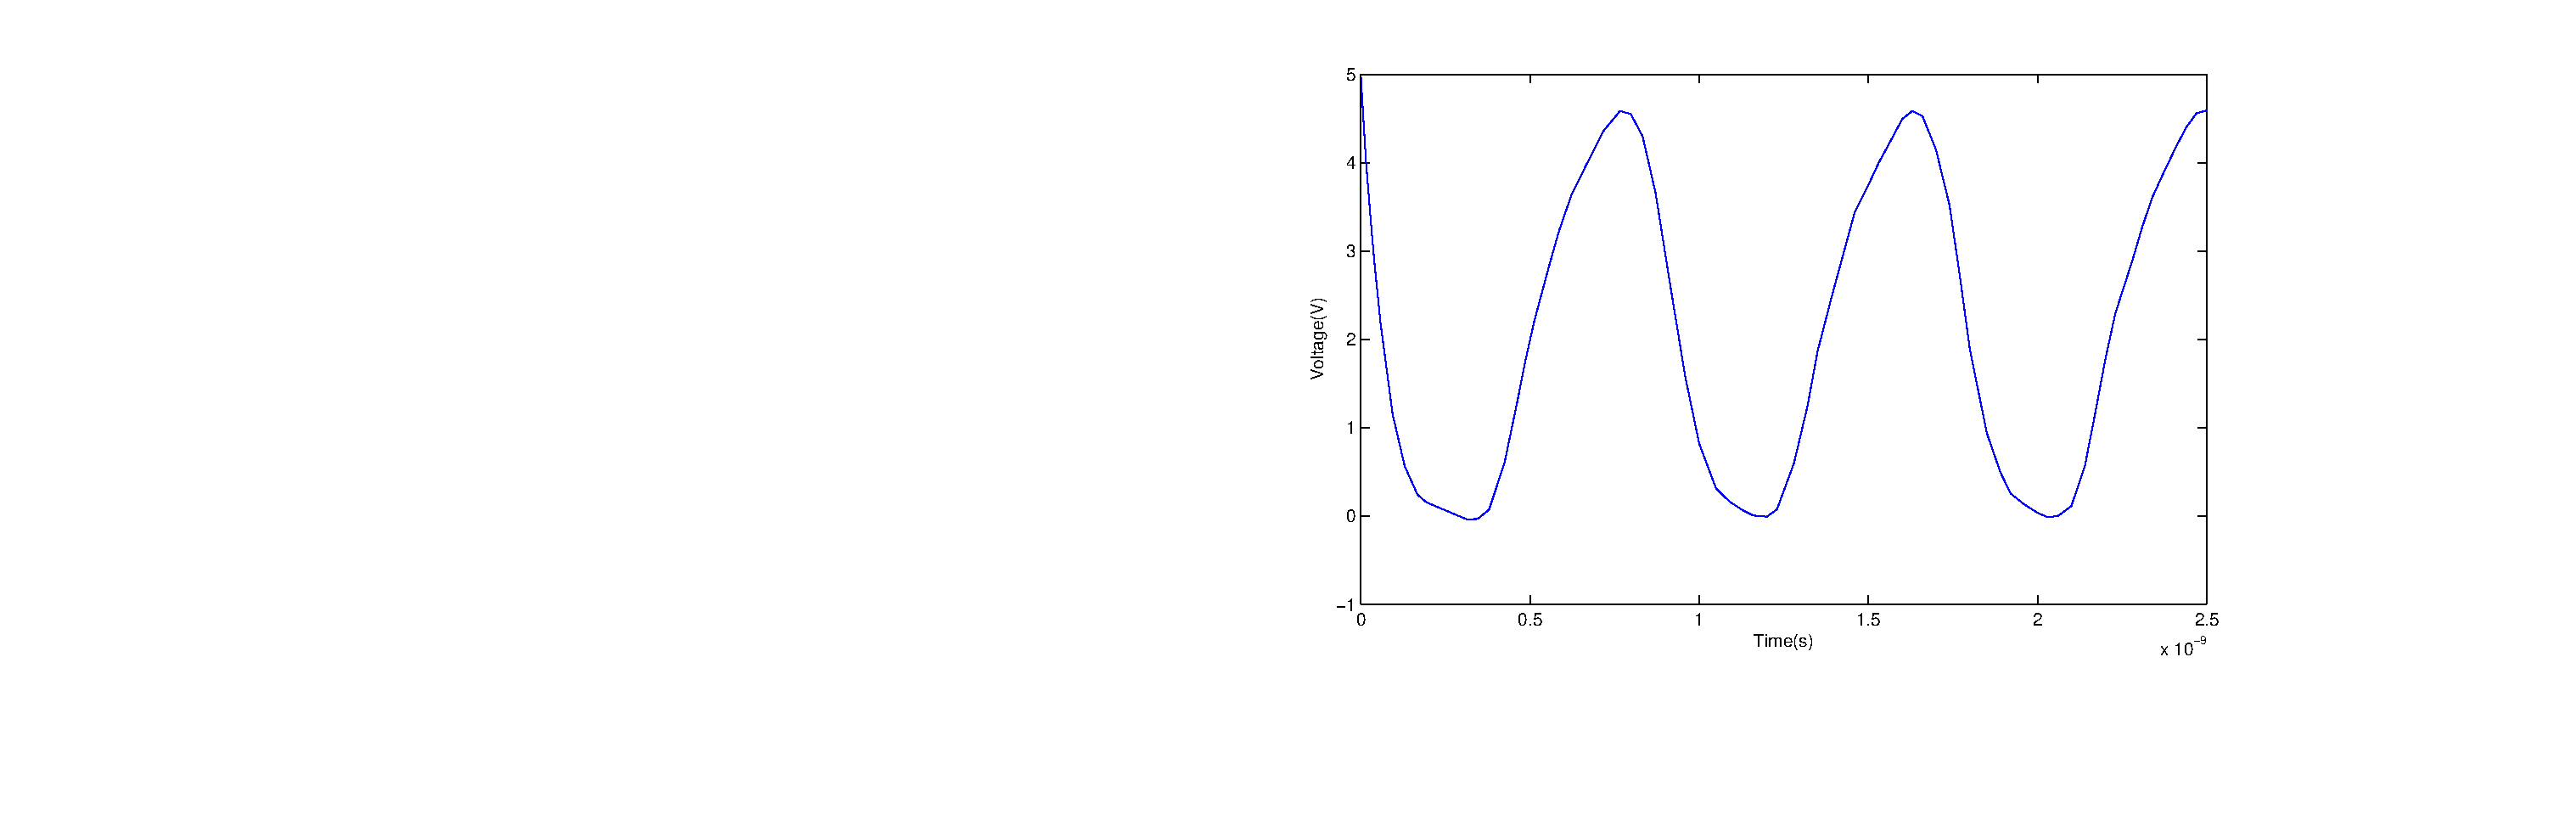
\includegraphics[width=\textwidth]{images/3-inverter-oscillator}
	\caption{Opbouw van een NMOS transistor.\cite{patel-slides}}
	\label{fig:NMOS-transistor}
\end{figure}

Wanneer er een spanningsverschil wordt gemaakt tussen de gate en de source zal er een depletiegebied ontstaan onder de gate. 
Dit depletiegebied zorgt ervoor dat er een stroom kan lopen tussen de source en de drain. 
Zie ook Figuur \ref{fig:depletiegebied}.
\begin{figure}[H]
\centering
	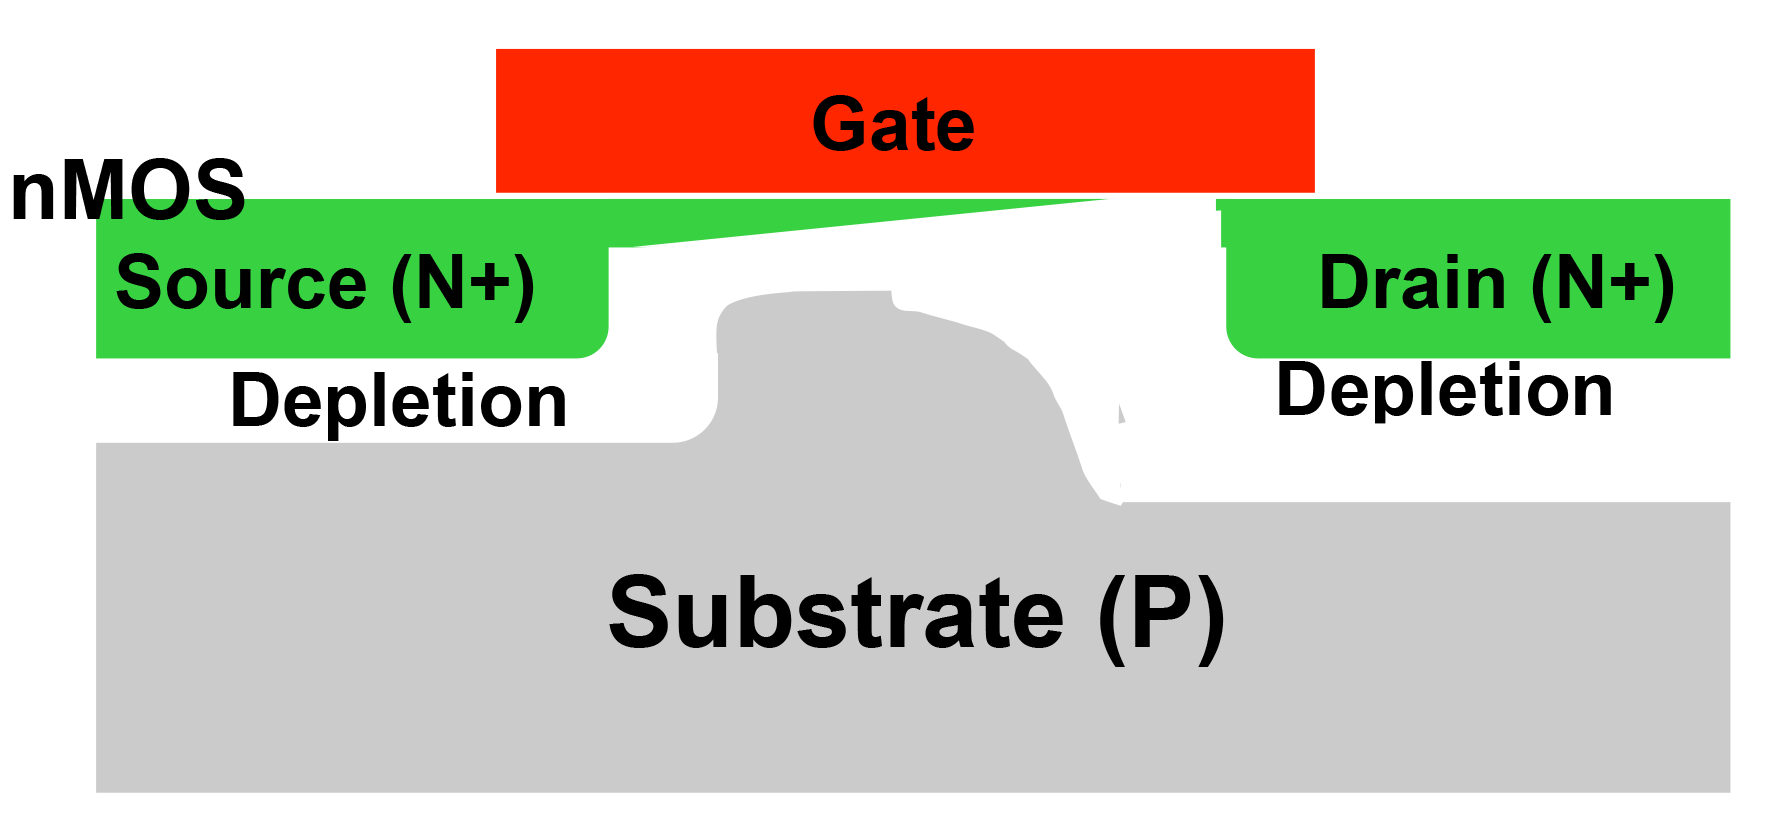
\includegraphics[width=\textwidth]{resources/depletiegebied}
	\caption{Een depletiegebied.\cite{nick-slides}}
	\label{fig:depletiegebied}
\end{figure}
Omdat we de drain hebben aangesloten op $V_{DS}$ en de source hebben aangesloten op de ground kan er nu ook daadwerkelijk stroom gaan lopen tussen source en drain. 
Als we het spanningsverschil over de gate en de source groter maken, zal ook het elektrisch veld groter worden, waardoor er meer stroom zal lopen. 
Dit gaat niet oneindig door. 
Voordat je de grens bereikt zit je in het resistieve of lineaire gebied en na de grens bevindt de transistor zich in het verzadigingsgebied. 
Wanneer de transistor zich in dit laatste gebied bevindt, zal er niet meer stroom gaan lopen naarmate het spanningsverschil toeneemt. 
De formule die we gebruiken om de stroom te berekenen in het verzadigingsgebied is:
\begin{equation}
I_{D} = k((V_{GS} - V_{T})(V_{GS} - V_{T}) - 0.5(V_{GS} - V_{T})^{2})
\end{equation}
\newline Dit is te vereenvoudigen tot: 
\begin{equation} I_{D} = 0.5k(V_{GS} - V_{T})^{2}
\end{equation}
\newline Voor het lineaire gebied gebruiken we de volgende formule: 
\begin{equation}
I_{D} = k(V_{GS} - V_{T})V_{DS} - 0.5V_{DS}^{2}
\end{equation}
\section{Simulaties}
Om de invloed van de verschillende $V_{GS}$ op de drainstroom van de NMOS transistor te bepalen, wanneer er ook nog sprake is van een oplopende waarde van $V_{DS}$, hebben we, met behulp van het programma PSpice, simulaties gemaakt. 
Het circuit wat voor de simulaties is gebruikt, is te zien in Figuur \ref{fig:circuit}. 

We hebben ervoor gekozen om in het circuit maar één NMOS transistor te gebruiken. 
We hadden er ook voor kunnen kiezen om meerdere transistoren parallel te plaatsen en daarover steeds een andere gate-source-spanning laten lopen. 
Dit hebben we echter niet gedaan, omdat bij zo'n circuit de transistors een kleine invloed op elkaar uitoefenen en dit zou kleine verschillen in de drainstroom tot gevolg kunnen hebben. 
Waarschijnlijk zouden de verschillen wel verwaarloosbaar klein zijn, maar toch hebben we het risico niet genomen. 
\\
Hoewel de NMOS transistor al beschreven was in een library (modellibEPO3.slb), moesten we wel nog zelf de kanaallengte en breedte van onze transistor invoeren. 
Voor onze simulatie moesten we werken met: \\
L = \unit{1.6}{\micro\meter} \\
W = \unit{4.8}{\micro\meter} \\
Na het circuit te hebben gesimuleerd moesten we er nog voor zorgen dat de werkgebieden van de transistor goed zichtbaar waren. 
Dit hebben we gedaan door 2 extra lijnen te tekenen, namelijk: 
\begin{enumerate}
	\item De lijn: 
\begin{equation}
V_{GS} - V_{T} = V_{DS} 
\end{equation}
	\item De lijn door alle buigpunten van de $I_{D}$ grafiek.
\end{enumerate}
Hoe deze lijnen precies tot stand zijn gekomen is te lezen in het volgende hoofdstuk. 


\begin{figure}[H]
\centering
	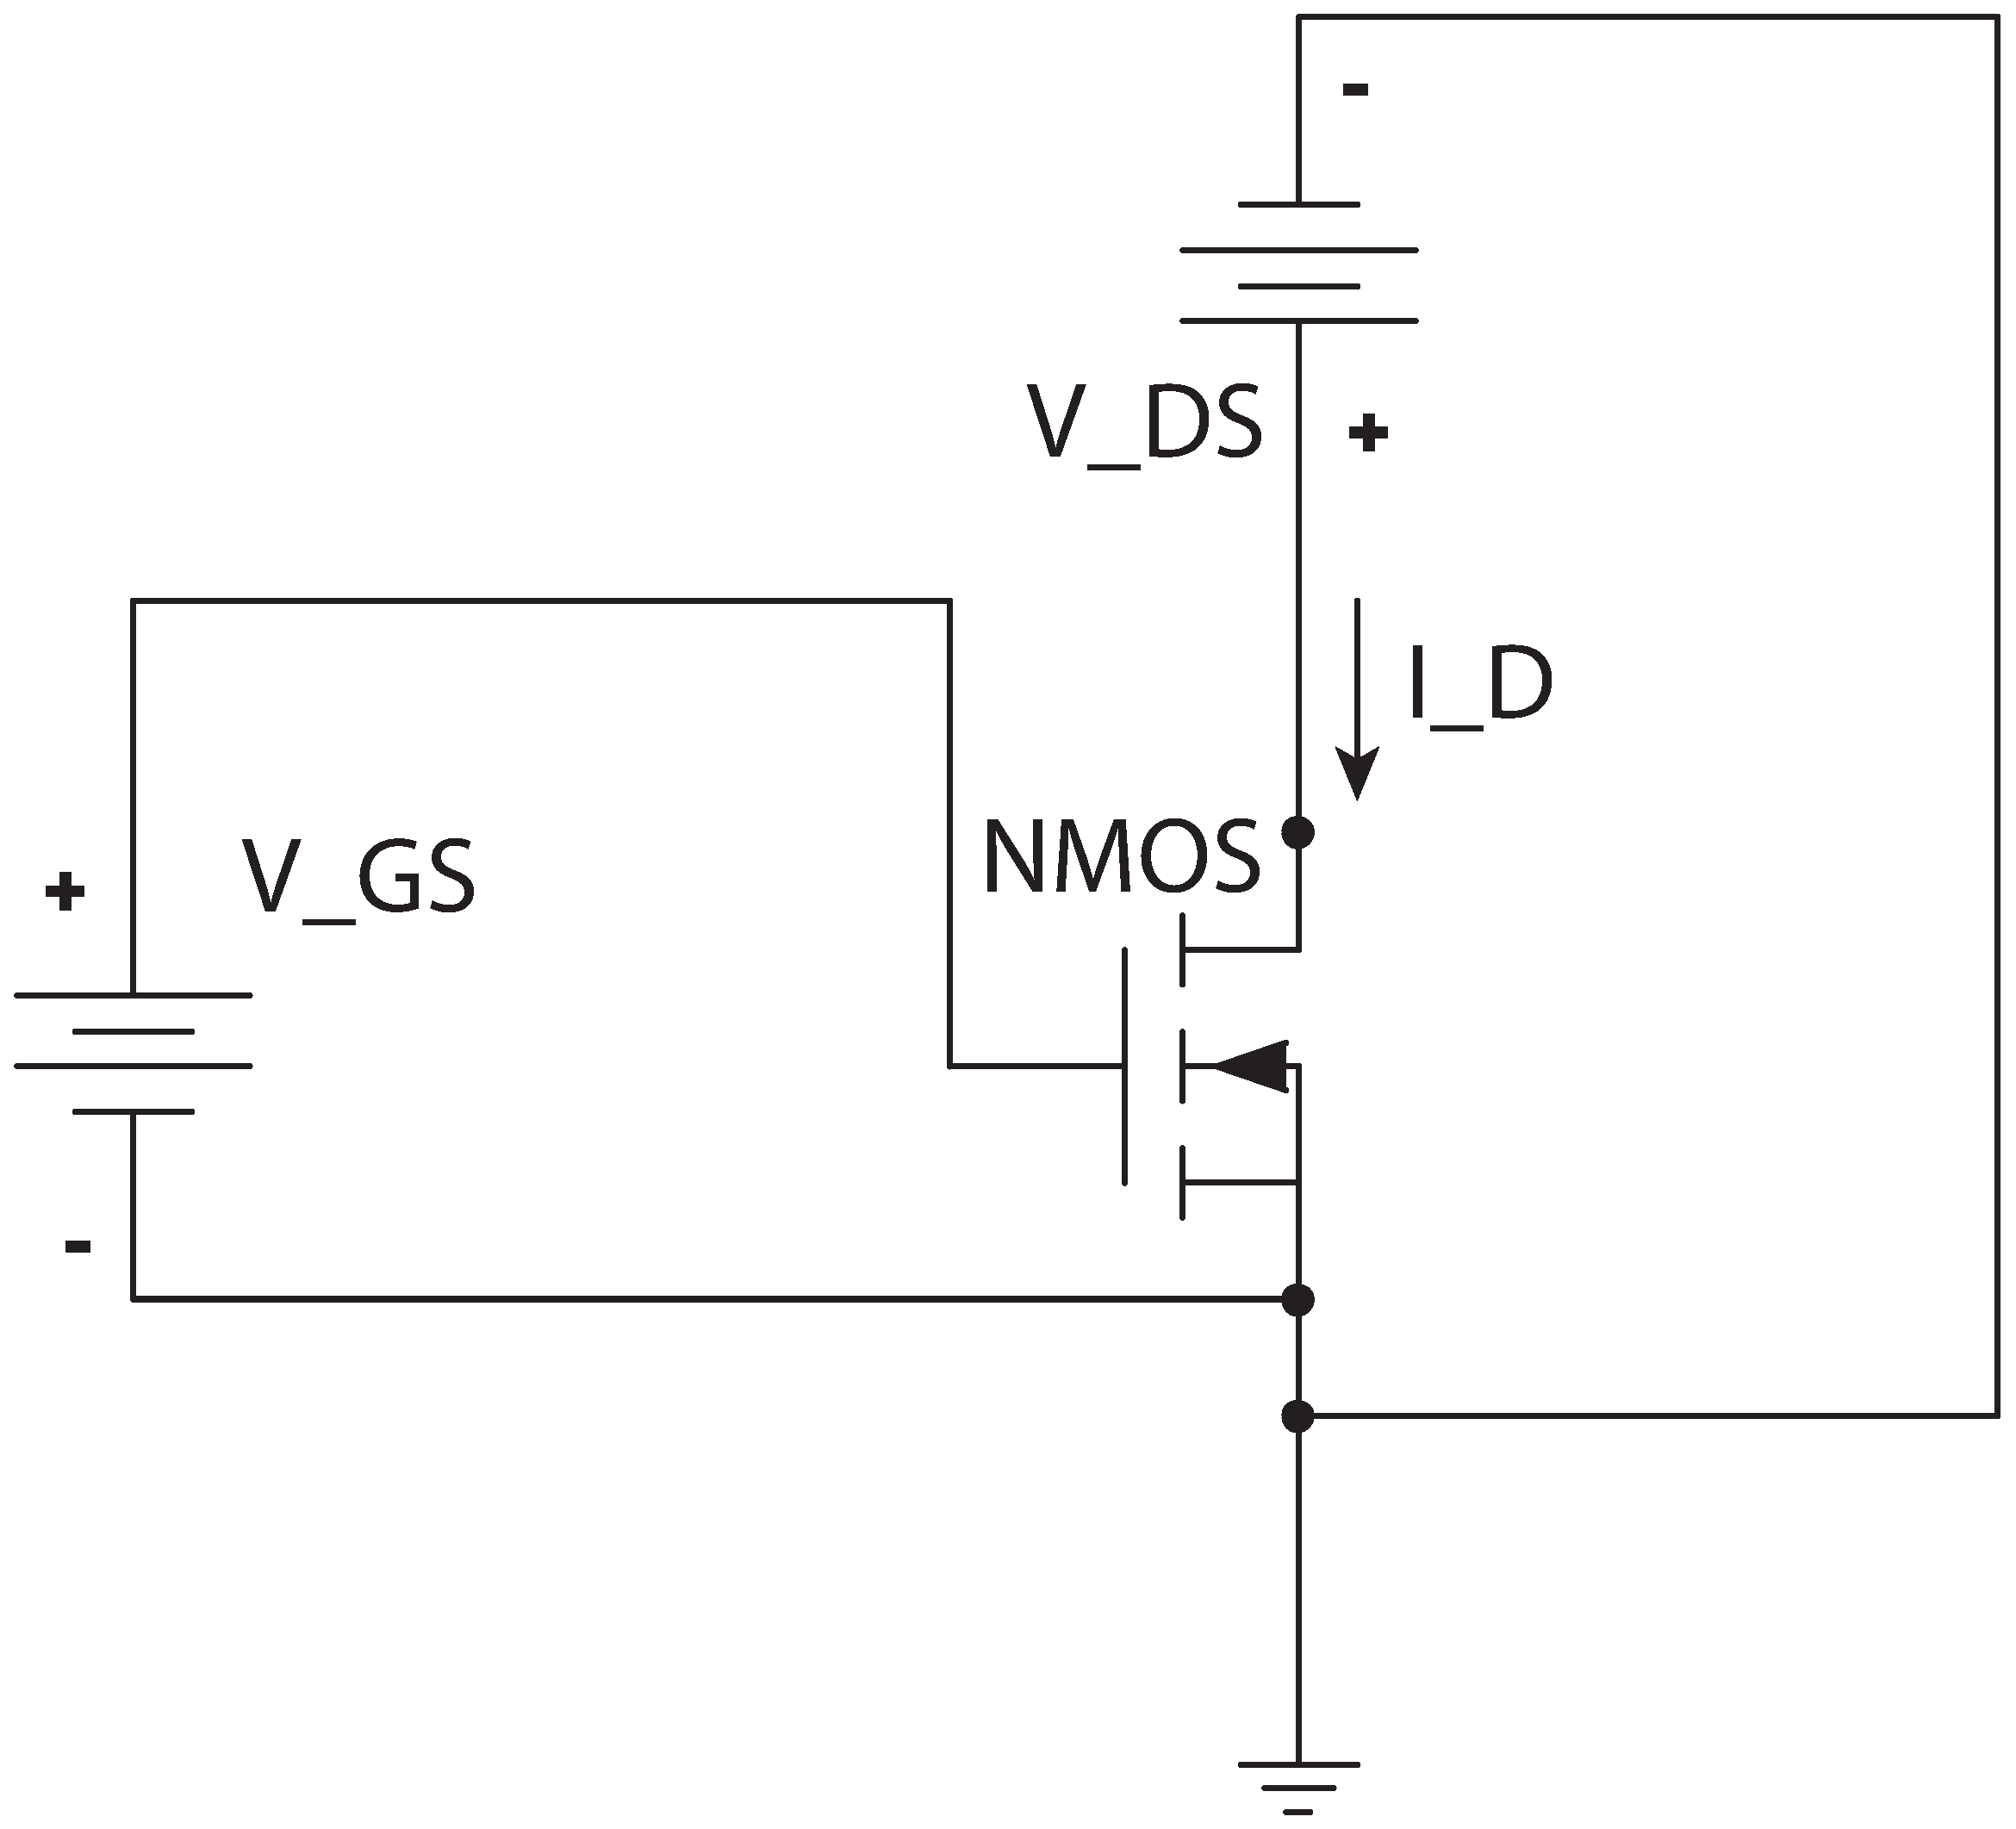
\includegraphics[width=0.8\textwidth]{resources/NMOS_circuit}
	\caption{Het circuit dat gebruikt is voor de simulaties.}
	\label{fig:circuit}
\end{figure}


\section{Resultaten}
Het resultaat van de simulatie van ons circuit ziet er als volgt uit.
\begin{figure}[H]
\centering
	\setlength\figureheight{0.6\textwidth} 
	\setlength\figurewidth{0.9\textwidth}
	% This file was created by matlab2tikz v0.4.2.
% Copyright (c) 2008--2013, Nico Schlömer <nico.schloemer@gmail.com>
% All rights reserved.
% 
% The latest updates can be retrieved from
%   http://www.mathworks.com/matlabcentral/fileexchange/22022-matlab2tikz
% where you can also make suggestions and rate matlab2tikz.
% 
% 
% 
%
% defining custom colors
\definecolor{mycolor1}{rgb}{0,0.75,0.75}%
\definecolor{mycolor2}{rgb}{0.75,0,0.75}%
\definecolor{mycolor3}{rgb}{0.75,0.75,0}%
%
\begin{tikzpicture}

\begin{axis}[%
width=\figurewidth,
height=\figureheight,
scale only axis,
xmin=0,
xmax=5,
xlabel={$\text{\$\$\mathsf}{\text{V}_{\text{DS}}}\text{\$\$}$},
ymin=0,
ymax=0.0014,
ylabel={$\text{\$\$\mathsf}{\text{I}_{\text{D}}}\text{\$\$}$},
legend style={at={(0.121164574616456,0.626170798898071)},anchor=south west,draw=black,fill=white,legend cell align=left}
]
\addplot [
color=blue,
solid,
line width=2.0pt
]
table[row sep=crcr]{
0 0\\
0.005 6.75779741275131e-15\\
0.01 1.32066099118385e-14\\
0.015 1.94007509439053e-14\\
0.02 2.53849845061483e-14\\
0.025 3.11962098948487e-14\\
0.03 3.68648389809448e-14\\
0.035 4.24159371634116e-14\\
0.04 4.78701652698987e-14\\
0.045 5.32445452745139e-14\\
0.05 5.85531175953911e-14\\
0.055 6.38074527025898e-14\\
0.06 6.90170780227005e-14\\
0.065 7.41898540214739e-14\\
0.07 7.93322655831541e-14\\
0.075 8.44496388509135e-14\\
0.08 8.95463783960777e-14\\
0.085 9.46261162959247e-14\\
0.09 9.96918408826923e-14\\
0.095 1.04746005163796e-13\\
0.1 1.09790655570836e-13\\
0.105 1.14827459064652e-13\\
0.11 1.19857777674225e-13\\
0.115 1.24882783693152e-13\\
0.12 1.29903385140753e-13\\
0.125 1.34920368063604e-13\\
0.13 1.39934369430481e-13\\
0.135 1.44945904237415e-13\\
0.14 1.49955406165275e-13\\
0.145 1.54963254684823e-13\\
0.15 1.59969707294073e-13\\
0.155 1.6497503504357e-13\\
0.16 1.69979427668693e-13\\
0.165 1.74983034247241e-13\\
0.17 1.79986017409539e-13\\
0.175 1.84988472023279e-13\\
0.18 1.89990506508676e-13\\
0.185 1.94992175075841e-13\\
0.19 1.99993545487408e-13\\
0.195 2.04994685506013e-13\\
0.2 2.09995622236711e-13\\
0.205 2.14996382784556e-13\\
0.21 2.19997021359657e-13\\
0.215 2.2499755151454e-13\\
0.22 2.29997986801733e-13\\
0.225 2.34998327221236e-13\\
0.23 2.39998613430631e-13\\
0.235 2.44998872534971e-13\\
0.24 2.49999077429203e-13\\
0.245 2.54999228113326e-13\\
0.25 2.59999378797449e-13\\
0.255 2.64999475271463e-13\\
0.26 2.70000005426346e-13\\
0.265 2.74999993480143e-13\\
0.27 2.80000008638995e-13\\
0.275 2.84999996692792e-13\\
0.28 2.90000011851643e-13\\
0.285 2.9499999990544e-13\\
0.29 2.99999987959237e-13\\
0.295 3.05000003118089e-13\\
0.3 3.09999991171886e-13\\
0.305 3.15000006330737e-13\\
0.31 3.19999994384534e-13\\
0.315 3.25000009543386e-13\\
0.32 3.29999997597183e-13\\
0.325 3.35000012756034e-13\\
0.33 3.40000000809831e-13\\
0.335 3.44999988863628e-13\\
0.34 3.5000000402248e-13\\
0.345 3.54999992076277e-13\\
0.35 3.60000007235128e-13\\
0.355 3.64999995288925e-13\\
0.36 3.70000010447777e-13\\
0.365 3.74999998501574e-13\\
0.37 3.79999986555371e-13\\
0.375 3.85000001714222e-13\\
0.38 3.8999998976802e-13\\
0.385 3.95000004926871e-13\\
0.39 3.99999992980668e-13\\
0.395 4.05000008139519e-13\\
0.4 4.09999996193317e-13\\
0.405 4.15000011352168e-13\\
0.41 4.19999999405965e-13\\
0.415 4.24999987459762e-13\\
0.42 4.30000002618613e-13\\
0.425 4.34999990672411e-13\\
0.43 4.40000005831262e-13\\
0.435 4.44999993885059e-13\\
0.44 4.5000000904391e-13\\
0.445 4.55000024202762e-13\\
0.45 4.59999985151505e-13\\
0.455 4.65000000310356e-13\\
0.46 4.70000015469207e-13\\
0.465 4.7499997641795e-13\\
0.47 4.79999991576802e-13\\
0.475 4.85000006735653e-13\\
0.48 4.90000021894504e-13\\
0.485 4.94999982843247e-13\\
0.49 4.99999998002099e-13\\
0.495 5.0500001316095e-13\\
0.5 5.09999974109693e-13\\
0.505 5.14999989268544e-13\\
0.51 5.20000004427396e-13\\
0.515 5.25000019586247e-13\\
0.52 5.2999998053499e-13\\
0.525 5.34999995693841e-13\\
0.53 5.40000010852693e-13\\
0.535 5.45000026011544e-13\\
0.54 5.49999986960287e-13\\
0.545 5.55000002119138e-13\\
0.55 5.6000001727799e-13\\
0.555 5.64999978226732e-13\\
0.56 5.69999993385584e-13\\
0.565 5.75000008544435e-13\\
0.57 5.80000023703287e-13\\
0.575 5.84999984652029e-13\\
0.58 5.89999999810881e-13\\
0.585 5.95000014969732e-13\\
0.59 5.99999975918475e-13\\
0.595 6.04999991077326e-13\\
0.6 6.10000006236178e-13\\
0.605 6.15000021395029e-13\\
0.61 6.19999982343772e-13\\
0.615 6.24999997502623e-13\\
0.62 6.30000012661475e-13\\
0.625 6.34999973610217e-13\\
0.63 6.39999988769069e-13\\
0.635 6.4500000392792e-13\\
0.64 6.50000019086772e-13\\
0.645 6.54999980035514e-13\\
0.65 6.59999995194366e-13\\
0.655 6.65000010353217e-13\\
0.66 6.70000025512069e-13\\
0.665 6.74999986460811e-13\\
0.67 6.80000001619663e-13\\
0.675 6.85000016778514e-13\\
0.68 6.89999977727257e-13\\
0.685000000000001 6.94999992886108e-13\\
0.690000000000001 7.0000000804496e-13\\
0.695000000000001 7.05000023203811e-13\\
0.700000000000001 7.09999984152554e-13\\
0.705000000000001 7.14999999311405e-13\\
0.710000000000001 7.20000014470257e-13\\
0.715000000000001 7.24999975419e-13\\
0.720000000000001 7.29999990577851e-13\\
0.725000000000001 7.35000005736702e-13\\
0.730000000000001 7.40000020895554e-13\\
0.735000000000001 7.44999981844297e-13\\
0.740000000000001 7.49999997003148e-13\\
0.745000000000001 7.55000012161999e-13\\
0.750000000000001 7.59999973110742e-13\\
0.755000000000001 7.64999988269593e-13\\
0.760000000000001 7.70000003428445e-13\\
0.765000000000001 7.75000018587296e-13\\
0.770000000000001 7.79999979536039e-13\\
0.775000000000001 7.8499999469489e-13\\
0.780000000000001 7.90000009853742e-13\\
0.785000000000001 7.95000025012593e-13\\
0.790000000000001 7.99999985961336e-13\\
0.795000000000001 8.05000001120187e-13\\
0.800000000000001 8.10000016279039e-13\\
0.805000000000001 8.14999977227782e-13\\
0.810000000000001 8.19999992386633e-13\\
0.815000000000001 8.25000007545484e-13\\
0.820000000000001 8.30000022704336e-13\\
0.825000000000001 8.34999983653079e-13\\
0.830000000000001 8.3999999881193e-13\\
0.835000000000001 8.45000013970781e-13\\
0.840000000000001 8.49999974919524e-13\\
0.845000000000001 8.54999990078376e-13\\
0.850000000000001 8.60000005237227e-13\\
0.855000000000001 8.65000020396078e-13\\
0.860000000000001 8.69999981344821e-13\\
0.865000000000001 8.74999996503673e-13\\
0.870000000000001 8.80000011662524e-13\\
0.875000000000001 8.85000026821375e-13\\
0.880000000000001 8.89999987770118e-13\\
0.885000000000001 8.9500000292897e-13\\
0.890000000000001 9.00000018087821e-13\\
0.895000000000001 9.04999979036564e-13\\
0.900000000000001 9.10000048405524e-13\\
0.905000000000001 9.14999955144158e-13\\
0.910000000000001 9.19999970303009e-13\\
0.915000000000001 9.24999985461861e-13\\
0.920000000000001 9.30000000620712e-13\\
0.925000000000001 9.35000015779563e-13\\
0.930000000000001 9.40000030938415e-13\\
0.935000000000001 9.45000046097266e-13\\
0.940000000000001 9.499999528359e-13\\
0.945000000000001 9.54999967994752e-13\\
0.950000000000001 9.59999983153603e-13\\
0.955000000000001 9.64999998312455e-13\\
0.960000000000001 9.70000013471306e-13\\
0.965000000000001 9.75000028630157e-13\\
0.970000000000001 9.80000043789009e-13\\
0.975000000000001 9.84999950527643e-13\\
0.980000000000001 9.89999965686494e-13\\
0.985000000000001 9.94999980845346e-13\\
0.990000000000001 9.99999996004197e-13\\
0.995000000000001 1.00500001116305e-12\\
1 1.0100000263219e-12\\
1.005 1.01500004148075e-12\\
1.01 1.01999994821939e-12\\
1.015 1.02499996337824e-12\\
1.02 1.02999997853709e-12\\
1.025 1.03499999369594e-12\\
1.03 1.04000000885479e-12\\
1.035 1.04500002401364e-12\\
1.04 1.05000003917249e-12\\
1.045 1.05499994591113e-12\\
1.05 1.05999996106998e-12\\
1.055 1.06499997622883e-12\\
1.06 1.06999999138768e-12\\
1.065 1.07500000654653e-12\\
1.07 1.08000002170539e-12\\
1.075 1.08500003686424e-12\\
1.08 1.09000005202309e-12\\
1.085 1.09499995876172e-12\\
1.09 1.09999997392057e-12\\
1.095 1.10499998907942e-12\\
1.1 1.11000000423828e-12\\
1.105 1.11500001939713e-12\\
1.11 1.12000003455598e-12\\
1.115 1.12500004971483e-12\\
1.12 1.12999995645346e-12\\
1.125 1.13499997161232e-12\\
1.13 1.13999998677117e-12\\
1.135 1.14500000193002e-12\\
1.14 1.15000001708887e-12\\
1.145 1.15500003224772e-12\\
1.15 1.16000004740657e-12\\
1.155 1.16499995414521e-12\\
1.16 1.16999996930406e-12\\
1.165 1.17499998446291e-12\\
1.17 1.17999999962176e-12\\
1.175 1.18500001478061e-12\\
1.18 1.19000002993946e-12\\
1.185 1.19500004509832e-12\\
1.19 1.19999995183695e-12\\
1.195 1.2049999669958e-12\\
1.2 1.20999998215465e-12\\
1.205 1.2149999973135e-12\\
1.21 1.22000001247236e-12\\
1.215 1.22500002763121e-12\\
1.22 1.23000004279006e-12\\
1.225 1.23499994952869e-12\\
1.23 1.23999996468754e-12\\
1.235 1.2449999798464e-12\\
1.24 1.24999999500525e-12\\
1.245 1.2550000101641e-12\\
1.25 1.26000002532295e-12\\
1.255 1.2650000404818e-12\\
1.26 1.26999994722043e-12\\
1.265 1.27499996237929e-12\\
1.26999999999999 1.27999997753814e-12\\
1.27499999999999 1.28499999269699e-12\\
1.27999999999999 1.29000000785584e-12\\
1.28499999999999 1.29500002301469e-12\\
1.28999999999999 1.30000003817354e-12\\
1.29499999999999 1.30500005333239e-12\\
1.29999999999999 1.30999996007103e-12\\
1.30499999999999 1.31499997522988e-12\\
1.30999999999999 1.31999999038873e-12\\
1.31499999999999 1.32500000554758e-12\\
1.31999999999999 1.33000002070643e-12\\
1.32499999999999 1.33500003586529e-12\\
1.32999999999999 1.34000005102414e-12\\
1.33499999999999 1.34499995776277e-12\\
1.33999999999999 1.34999997292162e-12\\
1.34499999999999 1.35499998808047e-12\\
1.34999999999999 1.36000000323933e-12\\
1.35499999999999 1.36500001839818e-12\\
1.35999999999999 1.37000003355703e-12\\
1.36499999999999 1.37500004871588e-12\\
1.36999999999999 1.37999995545451e-12\\
1.37499999999999 1.38499997061337e-12\\
1.37999999999999 1.38999998577222e-12\\
1.38499999999999 1.39500000093107e-12\\
1.38999999999999 1.40000001608992e-12\\
1.39499999999999 1.40500003124877e-12\\
1.39999999999999 1.41000004640762e-12\\
1.40499999999999 1.41499995314626e-12\\
1.40999999999999 1.41999996830511e-12\\
1.41499999999999 1.42499998346396e-12\\
1.41999999999999 1.42999999862281e-12\\
1.42499999999999 1.43500001378166e-12\\
1.42999999999999 1.44000002894051e-12\\
1.43499999999999 1.44500004409936e-12\\
1.43999999999999 1.449999950838e-12\\
1.44499999999999 1.45499996599685e-12\\
1.44999999999999 1.4599999811557e-12\\
1.45499999999999 1.46499999631455e-12\\
1.45999999999999 1.4700000114734e-12\\
1.46499999999999 1.47500002663226e-12\\
1.46999999999999 1.48000004179111e-12\\
1.47499999999999 1.48499994852974e-12\\
1.47999999999999 1.48999996368859e-12\\
1.48499999999999 1.49499997884744e-12\\
1.48999999999999 1.4999999940063e-12\\
1.49499999999999 1.50500000916515e-12\\
1.49999999999999 1.510000024324e-12\\
1.50499999999999 1.51500003948285e-12\\
1.50999999999999 1.51999994622148e-12\\
1.51499999999999 1.52499996138034e-12\\
1.51999999999999 1.52999997653919e-12\\
1.52499999999999 1.53499999169804e-12\\
1.52999999999999 1.54000000685689e-12\\
1.53499999999999 1.54500002201574e-12\\
1.53999999999999 1.55000003717459e-12\\
1.54499999999999 1.55500005233344e-12\\
1.54999999999999 1.55999995907208e-12\\
1.55499999999999 1.56499997423093e-12\\
1.55999999999999 1.56999998938978e-12\\
1.56499999999999 1.57500000454863e-12\\
1.56999999999999 1.58000001970748e-12\\
1.57499999999999 1.58500003486634e-12\\
1.57999999999999 1.59000005002519e-12\\
1.58499999999999 1.59499995676382e-12\\
1.58999999999999 1.59999997192267e-12\\
1.59499999999999 1.60499998708152e-12\\
1.59999999999999 1.61000000224037e-12\\
1.60499999999999 1.61500001739923e-12\\
1.60999999999999 1.62000003255808e-12\\
1.61499999999999 1.62500004771693e-12\\
1.61999999999999 1.62999995445556e-12\\
1.62499999999999 1.63499996961441e-12\\
1.62999999999999 1.63999998477327e-12\\
1.63499999999999 1.64499999993212e-12\\
1.63999999999999 1.65000001509097e-12\\
1.64499999999999 1.65500003024982e-12\\
1.64999999999999 1.66000004540867e-12\\
1.65499999999999 1.66499995214731e-12\\
1.65999999999999 1.66999996730616e-12\\
1.66499999999999 1.67499998246501e-12\\
1.66999999999999 1.67999999762386e-12\\
1.67499999999999 1.68500001278271e-12\\
1.67999999999999 1.69000002794156e-12\\
1.68499999999999 1.69500004310041e-12\\
1.68999999999999 1.69999994983905e-12\\
1.69499999999999 1.7049999649979e-12\\
1.69999999999999 1.70999998015675e-12\\
1.70499999999999 1.7149999953156e-12\\
1.70999999999999 1.72000001047445e-12\\
1.71499999999999 1.72500002563331e-12\\
1.71999999999999 1.73000004079216e-12\\
1.72499999999999 1.73499994753079e-12\\
1.72999999999999 1.73999996268964e-12\\
1.73499999999999 1.74499997784849e-12\\
1.73999999999998 1.74999999300735e-12\\
1.74499999999998 1.7550000081662e-12\\
1.74999999999998 1.76000002332505e-12\\
1.75499999999998 1.7650000384839e-12\\
1.75999999999998 1.77000005364275e-12\\
1.76499999999998 1.77499996038138e-12\\
1.76999999999998 1.77999997554024e-12\\
1.77499999999998 1.78499999069909e-12\\
1.77999999999998 1.79000000585794e-12\\
1.78499999999998 1.79500002101679e-12\\
1.78999999999998 1.80000003617564e-12\\
1.79499999999998 1.80500005133449e-12\\
1.79999999999998 1.80999995807313e-12\\
1.80499999999998 1.81499997323198e-12\\
1.80999999999998 1.82000009681105e-12\\
1.81499999999998 1.82500000354968e-12\\
1.81999999999998 1.82999991028832e-12\\
1.82499999999998 1.83500003386738e-12\\
1.82999999999998 1.83999994060602e-12\\
1.83499999999998 1.84500006418509e-12\\
1.83999999999998 1.84999997092372e-12\\
1.84499999999998 1.85500009450279e-12\\
1.84999999999998 1.86000000124142e-12\\
1.85499999999998 1.86499990798006e-12\\
1.85999999999998 1.87000003155913e-12\\
1.86499999999998 1.87499993829776e-12\\
1.86999999999998 1.88000006187683e-12\\
1.87499999999998 1.88499996861546e-12\\
1.87999999999998 1.89000009219453e-12\\
1.88499999999998 1.89499999893317e-12\\
1.88999999999998 1.8999999056718e-12\\
1.89499999999998 1.90500002925087e-12\\
1.89999999999998 1.9099999359895e-12\\
1.90499999999998 1.91500005956857e-12\\
1.90999999999998 1.91999996630721e-12\\
1.91499999999998 1.92500008988628e-12\\
1.91999999999998 1.92999999662491e-12\\
1.92499999999998 1.93499990336354e-12\\
1.92999999999998 1.94000002694261e-12\\
1.93499999999998 1.94499993368125e-12\\
1.93999999999998 1.95000005726031e-12\\
1.94499999999998 1.95499996399895e-12\\
1.94999999999998 1.96000008757802e-12\\
1.95499999999998 1.96499999431665e-12\\
1.95999999999998 1.96999990105529e-12\\
1.96499999999998 1.97500002463435e-12\\
1.96999999999998 1.97999993137299e-12\\
1.97499999999998 1.98500005495206e-12\\
1.97999999999998 1.98999996169069e-12\\
1.98499999999998 1.99500008526976e-12\\
1.98999999999998 1.99999999200839e-12\\
1.99499999999998 2.00499989874703e-12\\
1.99999999999998 2.0100000223261e-12\\
2.00499999999998 2.01499992906473e-12\\
2.00999999999998 2.0200000526438e-12\\
2.01499999999998 2.02499995938243e-12\\
2.01999999999998 2.0300000829615e-12\\
2.02499999999998 2.03499998970014e-12\\
2.02999999999998 2.03999989643877e-12\\
2.03499999999998 2.04500002001784e-12\\
2.03999999999998 2.04999992675647e-12\\
2.04499999999998 2.05500005033554e-12\\
2.04999999999998 2.05999995707418e-12\\
2.05499999999998 2.06500008065325e-12\\
2.05999999999998 2.06999998739188e-12\\
2.06499999999998 2.07499989413051e-12\\
2.06999999999998 2.08000001770958e-12\\
2.07499999999998 2.08499992444822e-12\\
2.07999999999998 2.09000004802729e-12\\
2.08499999999998 2.09499995476592e-12\\
2.08999999999998 2.10000007834499e-12\\
2.09499999999998 2.10499998508362e-12\\
2.09999999999998 2.10999989182226e-12\\
2.10499999999998 2.11500001540132e-12\\
2.10999999999998 2.11999992213996e-12\\
2.11499999999998 2.12500004571903e-12\\
2.11999999999998 2.12999995245766e-12\\
2.12499999999998 2.13500007603673e-12\\
2.12999999999998 2.13999998277536e-12\\
2.13499999999998 2.14500010635443e-12\\
2.13999999999998 2.15000001309307e-12\\
2.14499999999998 2.1549999198317e-12\\
2.14999999999998 2.16000004341077e-12\\
2.15499999999998 2.1649999501494e-12\\
2.15999999999998 2.17000007372847e-12\\
2.16499999999998 2.17499998046711e-12\\
2.16999999999998 2.18000010404618e-12\\
2.17499999999998 2.18500001078481e-12\\
2.17999999999998 2.18999991752344e-12\\
2.18499999999998 2.19500004110251e-12\\
2.18999999999998 2.19999994784115e-12\\
2.19499999999998 2.20500007142022e-12\\
2.19999999999998 2.20999997815885e-12\\
2.20499999999998 2.21500010173792e-12\\
2.20999999999998 2.22000000847655e-12\\
2.21499999999998 2.22499991521519e-12\\
2.21999999999997 2.23000003879426e-12\\
2.22499999999997 2.23499994553289e-12\\
2.22999999999997 2.24000006911196e-12\\
2.23499999999997 2.24499997585059e-12\\
2.23999999999997 2.25000009942966e-12\\
2.24499999999997 2.2550000061683e-12\\
2.24999999999997 2.25999991290693e-12\\
2.25499999999997 2.265000036486e-12\\
2.25999999999997 2.26999994322463e-12\\
2.26499999999997 2.2750000668037e-12\\
2.26999999999997 2.27999997354233e-12\\
2.27499999999997 2.2850000971214e-12\\
2.27999999999997 2.29000000386004e-12\\
2.28499999999997 2.29499991059867e-12\\
2.28999999999997 2.30000003417774e-12\\
2.29499999999997 2.30499994091637e-12\\
2.29999999999997 2.31000006449544e-12\\
2.30499999999997 2.31499997123408e-12\\
2.30999999999997 2.32000009481315e-12\\
2.31499999999997 2.32500000155178e-12\\
2.31999999999997 2.32999990829041e-12\\
2.32499999999997 2.33500003186948e-12\\
2.32999999999997 2.33999993860812e-12\\
2.33499999999997 2.34500006218719e-12\\
2.33999999999997 2.34999996892582e-12\\
2.34499999999997 2.35500009250489e-12\\
2.34999999999997 2.35999999924352e-12\\
2.35499999999997 2.36499990598216e-12\\
2.35999999999997 2.37000002956123e-12\\
2.36499999999997 2.37499993629986e-12\\
2.36999999999997 2.38000005987893e-12\\
2.37499999999997 2.38499996661756e-12\\
2.37999999999997 2.39000009019663e-12\\
2.38499999999997 2.39499999693527e-12\\
2.38999999999997 2.3999999036739e-12\\
2.39499999999997 2.40500002725297e-12\\
2.39999999999997 2.4099999339916e-12\\
2.40499999999997 2.41500005757067e-12\\
2.40999999999997 2.41999996430931e-12\\
2.41499999999997 2.42500008788837e-12\\
2.41999999999997 2.42999999462701e-12\\
2.42499999999997 2.43499990136564e-12\\
2.42999999999997 2.44000002494471e-12\\
2.43499999999997 2.44499993168334e-12\\
2.43999999999997 2.45000005526241e-12\\
2.44499999999997 2.45499996200105e-12\\
2.44999999999997 2.46000008558012e-12\\
2.45499999999997 2.46499999231875e-12\\
2.45999999999997 2.46999989905738e-12\\
2.46499999999997 2.47500002263645e-12\\
2.46999999999997 2.47999992937509e-12\\
2.47499999999997 2.48500005295416e-12\\
2.47999999999997 2.48999995969279e-12\\
2.48499999999997 2.49500008327186e-12\\
2.48999999999997 2.49999999001049e-12\\
2.49499999999997 2.50499989674913e-12\\
2.49999999999997 2.5100000203282e-12\\
2.50499999999997 2.51499992706683e-12\\
2.50999999999997 2.5200000506459e-12\\
2.51499999999997 2.52499995738453e-12\\
2.51999999999997 2.5300000809636e-12\\
2.52499999999997 2.53499998770224e-12\\
2.52999999999997 2.53999989444087e-12\\
2.53499999999997 2.54500001801994e-12\\
2.53999999999997 2.54999992475857e-12\\
2.54499999999997 2.55500004833764e-12\\
2.54999999999997 2.55999995507628e-12\\
2.55499999999997 2.56500007865534e-12\\
2.55999999999997 2.56999998539398e-12\\
2.56499999999997 2.57499989213261e-12\\
2.56999999999997 2.58000001571168e-12\\
2.57499999999997 2.58499992245032e-12\\
2.57999999999997 2.59000004602938e-12\\
2.58499999999997 2.59499995276802e-12\\
2.58999999999997 2.60000007634709e-12\\
2.59499999999997 2.60499998308572e-12\\
2.59999999999997 2.61000010666479e-12\\
2.60499999999997 2.61500001340342e-12\\
2.60999999999997 2.61999992014206e-12\\
2.61499999999997 2.62500004372113e-12\\
2.61999999999997 2.62999995045976e-12\\
2.62499999999997 2.63500007403883e-12\\
2.62999999999997 2.63999998077746e-12\\
2.63499999999997 2.64500010435653e-12\\
2.63999999999997 2.65000001109517e-12\\
2.64499999999997 2.6549999178338e-12\\
2.64999999999997 2.66000004141287e-12\\
2.65499999999997 2.6649999481515e-12\\
2.65999999999997 2.67000007173057e-12\\
2.66499999999997 2.67499997846921e-12\\
2.66999999999997 2.68000010204827e-12\\
2.67499999999997 2.68500000878691e-12\\
2.67999999999997 2.68999991552554e-12\\
2.68499999999997 2.69500003910461e-12\\
2.68999999999996 2.69999994584325e-12\\
2.69499999999996 2.70500006942231e-12\\
2.69999999999996 2.70999997616095e-12\\
2.70499999999996 2.71500009974002e-12\\
2.70999999999996 2.72000000647865e-12\\
2.71499999999996 2.72499991321729e-12\\
2.71999999999996 2.73000003679635e-12\\
2.72499999999996 2.73499994353499e-12\\
2.72999999999996 2.74000006711406e-12\\
2.73499999999996 2.74499997385269e-12\\
2.73999999999996 2.75000009743176e-12\\
2.74499999999996 2.75500000417039e-12\\
2.74999999999996 2.75999991090903e-12\\
2.75499999999996 2.7650000344881e-12\\
2.75999999999996 2.76999994122673e-12\\
2.76499999999996 2.7750000648058e-12\\
2.76999999999996 2.77999997154443e-12\\
2.77499999999996 2.7850000951235e-12\\
2.77999999999996 2.79000000186214e-12\\
2.78499999999996 2.79499990860077e-12\\
2.78999999999996 2.80000003217984e-12\\
2.79499999999996 2.80499993891847e-12\\
2.79999999999996 2.81000006249754e-12\\
2.80499999999996 2.81499996923618e-12\\
2.80999999999996 2.82000009281524e-12\\
2.81499999999996 2.82499999955388e-12\\
2.81999999999996 2.82999990629251e-12\\
2.82499999999996 2.83500002987158e-12\\
2.82999999999996 2.83999993661022e-12\\
2.83499999999996 2.84500006018928e-12\\
2.83999999999996 2.84999996692792e-12\\
2.84499999999996 2.85500009050699e-12\\
2.84999999999996 2.85999999724562e-12\\
2.85499999999996 2.86499990398426e-12\\
2.85999999999996 2.87000002756332e-12\\
2.86499999999996 2.87499993430196e-12\\
2.86999999999996 2.88000005788103e-12\\
2.87499999999996 2.88499996461966e-12\\
2.87999999999996 2.89000008819873e-12\\
2.88499999999996 2.89499999493736e-12\\
2.88999999999996 2.899999901676e-12\\
2.89499999999996 2.90500002525507e-12\\
2.89999999999996 2.9099999319937e-12\\
2.90499999999996 2.91500005557277e-12\\
2.90999999999996 2.9199999623114e-12\\
2.91499999999996 2.92500008589047e-12\\
2.91999999999996 2.92999999262911e-12\\
2.92499999999996 2.93499989936774e-12\\
2.92999999999996 2.94000002294681e-12\\
2.93499999999996 2.94499992968544e-12\\
2.93999999999996 2.95000005326451e-12\\
2.94499999999996 2.95499996000315e-12\\
2.94999999999996 2.96000008358221e-12\\
2.95499999999996 2.96499999032085e-12\\
2.95999999999996 2.96999989705948e-12\\
2.96499999999996 2.97500002063855e-12\\
2.96999999999996 2.97999992737719e-12\\
2.97499999999996 2.98500005095625e-12\\
2.97999999999996 2.98999995769489e-12\\
2.98499999999996 2.99500008127396e-12\\
2.98999999999996 2.99999998801259e-12\\
2.99499999999996 3.00499989475123e-12\\
2.99999999999996 3.01000001833029e-12\\
3.00499999999996 3.01499992506893e-12\\
3.00999999999996 3.020000048648e-12\\
3.01499999999996 3.02499995538663e-12\\
3.01999999999996 3.0300000789657e-12\\
3.02499999999996 3.03499998570433e-12\\
3.02999999999996 3.03999989244297e-12\\
3.03499999999996 3.04500001602204e-12\\
3.03999999999996 3.04999992276067e-12\\
3.04499999999996 3.05500004633974e-12\\
3.04999999999996 3.05999995307837e-12\\
3.05499999999996 3.06500007665744e-12\\
3.05999999999996 3.06999998339608e-12\\
3.06499999999996 3.07500010697515e-12\\
3.06999999999996 3.08000001371378e-12\\
3.07499999999996 3.08499992045241e-12\\
3.07999999999996 3.09000004403148e-12\\
3.08499999999996 3.09499995077012e-12\\
3.08999999999996 3.10000007434919e-12\\
3.09499999999996 3.10499998108782e-12\\
3.09999999999996 3.11000010466689e-12\\
3.10499999999996 3.11500001140552e-12\\
3.10999999999996 3.11999991814416e-12\\
3.11499999999996 3.12500004172322e-12\\
3.11999999999996 3.12999994846186e-12\\
3.12499999999996 3.13500007204093e-12\\
3.12999999999996 3.13999997877956e-12\\
3.13499999999996 3.14500010235863e-12\\
3.13999999999996 3.15000000909726e-12\\
3.14499999999996 3.1549999158359e-12\\
3.14999999999996 3.16000003941497e-12\\
3.15499999999996 3.1649999461536e-12\\
3.15999999999995 3.17000006973267e-12\\
3.16499999999995 3.1749999764713e-12\\
3.16999999999995 3.18000010005037e-12\\
3.17499999999995 3.18500000678901e-12\\
3.17999999999995 3.18999991352764e-12\\
3.18499999999995 3.19500003710671e-12\\
3.18999999999995 3.19999994384534e-12\\
3.19499999999995 3.20500006742441e-12\\
3.19999999999995 3.20999997416305e-12\\
3.20499999999995 3.21500009774212e-12\\
3.20999999999995 3.22000000448075e-12\\
3.21499999999995 3.22499991121938e-12\\
3.21999999999995 3.23000003479845e-12\\
3.22499999999995 3.23499994153709e-12\\
3.22999999999995 3.24000006511616e-12\\
3.23499999999995 3.24499997185479e-12\\
3.23999999999995 3.25000009543386e-12\\
3.24499999999995 3.25500000217249e-12\\
3.24999999999995 3.25999990891113e-12\\
3.25499999999995 3.2650000324902e-12\\
3.25999999999995 3.26999993922883e-12\\
3.26499999999995 3.2750000628079e-12\\
3.26999999999995 3.27999996954653e-12\\
3.27499999999995 3.2850000931256e-12\\
3.27999999999995 3.28999999986423e-12\\
3.28499999999995 3.29499990660287e-12\\
3.28999999999995 3.30000003018194e-12\\
3.29499999999995 3.30499993692057e-12\\
3.29999999999995 3.31000006049964e-12\\
3.30499999999995 3.31499996723827e-12\\
3.30999999999995 3.32000009081734e-12\\
3.31499999999995 3.32499999755598e-12\\
3.31999999999995 3.32999990429461e-12\\
3.32499999999995 3.33500002787368e-12\\
3.32999999999995 3.33999993461231e-12\\
3.33499999999995 3.34500005819138e-12\\
3.33999999999995 3.34999996493002e-12\\
3.34499999999995 3.35500008850909e-12\\
3.34999999999995 3.35999999524772e-12\\
3.35499999999995 3.36499990198635e-12\\
3.35999999999995 3.37000002556542e-12\\
3.36499999999995 3.37499993230406e-12\\
3.36999999999995 3.38000005588313e-12\\
3.37499999999995 3.38499996262176e-12\\
3.37999999999995 3.39000008620083e-12\\
3.38499999999995 3.39499999293946e-12\\
3.38999999999995 3.3999998996781e-12\\
3.39499999999995 3.40500002325717e-12\\
3.39999999999995 3.4099999299958e-12\\
3.40499999999995 3.41500005357487e-12\\
3.40999999999995 3.4199999603135e-12\\
3.41499999999995 3.42500008389257e-12\\
3.41999999999995 3.42999999063121e-12\\
3.42499999999995 3.43499989736984e-12\\
3.42999999999995 3.44000002094891e-12\\
3.43499999999995 3.44499992768754e-12\\
3.43999999999995 3.45000005126661e-12\\
3.44499999999995 3.45499995800524e-12\\
3.44999999999995 3.46000008158431e-12\\
3.45499999999995 3.46499998832295e-12\\
3.45999999999995 3.46999989506158e-12\\
3.46499999999995 3.47500001864065e-12\\
3.46999999999995 3.47999992537928e-12\\
3.47499999999995 3.48500004895835e-12\\
3.47999999999995 3.48999995569699e-12\\
3.48499999999995 3.49500007927606e-12\\
3.48999999999995 3.49999998601469e-12\\
3.49499999999995 3.50499989275332e-12\\
3.49999999999995 3.51000001633239e-12\\
3.50499999999995 3.51499992307103e-12\\
3.50999999999995 3.5200000466501e-12\\
3.51499999999995 3.52499995338873e-12\\
3.51999999999995 3.5300000769678e-12\\
3.52499999999995 3.53499998370643e-12\\
3.52999999999995 3.5400001072855e-12\\
3.53499999999995 3.54500001402414e-12\\
3.53999999999995 3.54999992076277e-12\\
3.54499999999995 3.55500004434184e-12\\
3.54999999999995 3.55999995108047e-12\\
3.55499999999995 3.56500007465954e-12\\
3.55999999999995 3.56999998139818e-12\\
3.56499999999995 3.57500010497724e-12\\
3.56999999999995 3.58000001171588e-12\\
3.57499999999995 3.58499991845451e-12\\
3.57999999999995 3.59000004203358e-12\\
3.58499999999995 3.59499994877222e-12\\
3.58999999999995 3.60000007235128e-12\\
3.59499999999995 3.60499997908992e-12\\
3.59999999999995 3.61000010266899e-12\\
3.60499999999995 3.61500000940762e-12\\
3.60999999999995 3.61999991614625e-12\\
3.61499999999995 3.62500003972532e-12\\
3.61999999999995 3.62999994646396e-12\\
3.62499999999994 3.63500007004303e-12\\
3.62999999999994 3.64000019362209e-12\\
3.63499999999994 3.64500010036073e-12\\
3.63999999999994 3.65000000709936e-12\\
3.64499999999994 3.654999913838e-12\\
3.64999999999994 3.65999982057663e-12\\
3.65499999999994 3.66500016099613e-12\\
3.65999999999994 3.67000006773477e-12\\
3.66499999999994 3.6749999744734e-12\\
3.66999999999994 3.67999988121204e-12\\
3.67499999999994 3.68499978795067e-12\\
3.67999999999994 3.69000012837017e-12\\
3.68499999999994 3.69500003510881e-12\\
3.68999999999994 3.69999994184744e-12\\
3.69499999999994 3.70499984858608e-12\\
3.69999999999994 3.71000018900558e-12\\
3.70499999999994 3.71500009574421e-12\\
3.70999999999994 3.72000000248285e-12\\
3.71499999999994 3.72499990922148e-12\\
3.71999999999994 3.72999981596012e-12\\
3.72499999999994 3.73500015637962e-12\\
3.72999999999994 3.74000006311825e-12\\
3.73499999999994 3.74499996985689e-12\\
3.73999999999994 3.74999987659552e-12\\
3.74499999999994 3.75499978333416e-12\\
3.74999999999994 3.76000012375366e-12\\
3.75499999999994 3.76500003049229e-12\\
3.75999999999994 3.76999993723093e-12\\
3.76499999999994 3.77499984396956e-12\\
3.76999999999994 3.78000018438907e-12\\
3.77499999999994 3.7850000911277e-12\\
3.77999999999994 3.78999999786633e-12\\
3.78499999999994 3.79499990460497e-12\\
3.78999999999994 3.7999998113436e-12\\
3.79499999999994 3.8050001517631e-12\\
3.79999999999994 3.81000005850174e-12\\
3.80499999999994 3.81499996524037e-12\\
3.80999999999994 3.81999987197901e-12\\
3.81499999999994 3.82500021239851e-12\\
3.81999999999994 3.83000011913714e-12\\
3.82499999999994 3.83500002587578e-12\\
3.82999999999994 3.83999993261441e-12\\
3.83499999999994 3.84499983935305e-12\\
3.83999999999994 3.85000017977255e-12\\
3.84499999999994 3.85500008651118e-12\\
3.84999999999994 3.85999999324982e-12\\
3.85499999999994 3.86499989998845e-12\\
3.85999999999994 3.86999980672709e-12\\
3.86499999999994 3.87500014714659e-12\\
3.86999999999994 3.88000005388522e-12\\
3.87499999999994 3.88499996062386e-12\\
3.87999999999994 3.88999986736249e-12\\
3.88499999999994 3.895000207782e-12\\
3.88999999999994 3.90000011452063e-12\\
3.89499999999994 3.90500002125926e-12\\
3.89999999999994 3.9099999279979e-12\\
3.90499999999994 3.91499983473653e-12\\
3.90999999999994 3.92000017515604e-12\\
3.91499999999994 3.92500008189467e-12\\
3.91999999999994 3.9299999886333e-12\\
3.92499999999994 3.93499989537194e-12\\
3.92999999999994 3.93999980211057e-12\\
3.93499999999994 3.94500014253008e-12\\
3.93999999999994 3.95000004926871e-12\\
3.94499999999994 3.95499995600734e-12\\
3.94999999999994 3.95999986274598e-12\\
3.95499999999994 3.96500020316548e-12\\
3.95999999999994 3.97000010990411e-12\\
3.96499999999994 3.97500001664275e-12\\
3.96999999999994 3.97999992338138e-12\\
3.97499999999994 3.98499983012002e-12\\
3.97999999999994 3.99000017053952e-12\\
3.98499999999994 3.99500007727815e-12\\
3.98999999999994 3.99999998401679e-12\\
3.99499999999994 4.00499989075542e-12\\
3.99999999999994 4.00999979749406e-12\\
4.00499999999994 4.01500013791356e-12\\
4.00999999999994 4.02000004465219e-12\\
4.01499999999994 4.02499995139083e-12\\
4.01999999999994 4.02999985812946e-12\\
4.02499999999994 4.03500019854897e-12\\
4.02999999999994 4.0400001052876e-12\\
4.03499999999994 4.04500001202623e-12\\
4.03999999999994 4.04999991876487e-12\\
4.04499999999994 4.0549998255035e-12\\
4.04999999999994 4.06000016592301e-12\\
4.05499999999994 4.06500007266164e-12\\
4.05999999999994 4.06999997940027e-12\\
4.06499999999994 4.07499988613891e-12\\
4.06999999999994 4.07999979287754e-12\\
4.07499999999994 4.08500013329705e-12\\
4.07999999999994 4.09000004003568e-12\\
4.08499999999994 4.09499994677431e-12\\
4.08999999999994 4.09999985351295e-12\\
4.09499999999993 4.10500019393245e-12\\
4.09999999999993 4.11000010067109e-12\\
4.10499999999993 4.11500000740972e-12\\
4.10999999999993 4.11999991414835e-12\\
4.11499999999993 4.12499982088699e-12\\
4.11999999999993 4.13000016130649e-12\\
4.12499999999993 4.13500006804512e-12\\
4.12999999999993 4.13999997478376e-12\\
4.13499999999993 4.14499988152239e-12\\
4.13999999999993 4.14999978826103e-12\\
4.14499999999993 4.15500012868053e-12\\
4.14999999999993 4.16000003541916e-12\\
4.15499999999993 4.1649999421578e-12\\
4.15999999999993 4.16999984889643e-12\\
4.16499999999993 4.17500018931594e-12\\
4.16999999999993 4.18000009605457e-12\\
4.17499999999993 4.1850000027932e-12\\
4.17999999999993 4.18999990953184e-12\\
4.18499999999993 4.19499981627047e-12\\
4.18999999999993 4.20000015668998e-12\\
4.19499999999993 4.20500006342861e-12\\
4.19999999999993 4.20999997016724e-12\\
4.20499999999993 4.21499987690588e-12\\
4.20999999999993 4.21999978364451e-12\\
4.21499999999993 4.22500012406402e-12\\
4.21999999999993 4.23000003080265e-12\\
4.22499999999993 4.23499993754128e-12\\
4.22999999999993 4.23999984427992e-12\\
4.23499999999993 4.24500018469942e-12\\
4.23999999999993 4.25000009143806e-12\\
4.24499999999993 4.25499999817669e-12\\
4.24999999999993 4.25999990491532e-12\\
4.25499999999993 4.26499981165396e-12\\
4.25999999999993 4.27000015207346e-12\\
4.26499999999993 4.2750000588121e-12\\
4.26999999999993 4.27999996555073e-12\\
4.27499999999993 4.28499987228936e-12\\
4.27999999999993 4.29000021270887e-12\\
4.28499999999993 4.2950001194475e-12\\
4.28999999999993 4.30000002618613e-12\\
4.29499999999993 4.30499993292477e-12\\
4.29999999999993 4.3099998396634e-12\\
4.30499999999993 4.31500018008291e-12\\
4.30999999999993 4.32000008682154e-12\\
4.31499999999993 4.32499999356017e-12\\
4.31999999999993 4.32999990029881e-12\\
4.32499999999993 4.33499980703744e-12\\
4.32999999999993 4.34000014745695e-12\\
4.33499999999993 4.34500005419558e-12\\
4.33999999999993 4.34999996093421e-12\\
4.34499999999993 4.35499986767285e-12\\
4.34999999999993 4.36000020809235e-12\\
4.35499999999993 4.36500011483099e-12\\
4.35999999999993 4.37000002156962e-12\\
4.36499999999993 4.37499992830825e-12\\
4.36999999999993 4.37999983504689e-12\\
4.37499999999993 4.38500017546639e-12\\
4.37999999999993 4.39000008220503e-12\\
4.38499999999993 4.39499998894366e-12\\
4.38999999999993 4.39999989568229e-12\\
4.39499999999993 4.40499980242093e-12\\
4.39999999999993 4.41000014284043e-12\\
4.40499999999993 4.41500004957907e-12\\
4.40999999999993 4.4199999563177e-12\\
4.41499999999993 4.42499986305633e-12\\
4.41999999999993 4.43000020347584e-12\\
4.42499999999993 4.43500011021447e-12\\
4.42999999999993 4.44000001695311e-12\\
4.43499999999993 4.44499992369174e-12\\
4.43999999999993 4.44999983043037e-12\\
4.44499999999993 4.45500017084988e-12\\
4.44999999999993 4.46000007758851e-12\\
4.45499999999993 4.46499998432714e-12\\
4.45999999999993 4.46999989106578e-12\\
4.46499999999993 4.47499979780441e-12\\
4.46999999999993 4.48000013822392e-12\\
4.47499999999993 4.48500004496255e-12\\
4.47999999999993 4.48999995170118e-12\\
4.48499999999993 4.49499985843982e-12\\
4.48999999999993 4.50000019885932e-12\\
4.49499999999993 4.50500010559796e-12\\
4.49999999999993 4.51000001233659e-12\\
4.50499999999993 4.51499991907522e-12\\
4.50999999999993 4.51999982581386e-12\\
4.51499999999993 4.52500016623336e-12\\
4.51999999999993 4.530000072972e-12\\
4.52499999999993 4.53499997971063e-12\\
4.52999999999993 4.53999988644926e-12\\
4.53499999999993 4.5449997931879e-12\\
4.53999999999993 4.5500001336074e-12\\
4.54499999999993 4.55500004034604e-12\\
4.54999999999993 4.55999994708467e-12\\
4.55499999999993 4.5649998538233e-12\\
4.55999999999993 4.57000019424281e-12\\
4.56499999999992 4.57500010098144e-12\\
4.56999999999992 4.58000000772008e-12\\
4.57499999999992 4.58499991445871e-12\\
4.57999999999992 4.58999982119734e-12\\
4.58499999999992 4.59500016161685e-12\\
4.58999999999992 4.60000006835548e-12\\
4.59499999999992 4.60499997509412e-12\\
4.59999999999992 4.60999988183275e-12\\
4.60499999999992 4.61499978857138e-12\\
4.60999999999992 4.62000012899089e-12\\
4.61499999999992 4.62500003572952e-12\\
4.61999999999992 4.62999994246815e-12\\
4.62499999999992 4.63499984920679e-12\\
4.62999999999992 4.64000018962629e-12\\
4.63499999999992 4.64500009636493e-12\\
4.63999999999992 4.65000000310356e-12\\
4.64499999999992 4.65499990984219e-12\\
4.64999999999992 4.65999981658083e-12\\
4.65499999999992 4.66500015700033e-12\\
4.65999999999992 4.67000006373897e-12\\
4.66499999999992 4.6749999704776e-12\\
4.66999999999992 4.67999987721623e-12\\
4.67499999999992 4.68499978395487e-12\\
4.67999999999992 4.69000012437437e-12\\
4.68499999999992 4.69500003111301e-12\\
4.68999999999992 4.69999993785164e-12\\
4.69499999999992 4.70499984459027e-12\\
4.69999999999992 4.71000018500978e-12\\
4.70499999999992 4.71500009174841e-12\\
4.70999999999992 4.71999999848705e-12\\
4.71499999999992 4.72499990522568e-12\\
4.71999999999992 4.72999981196431e-12\\
4.72499999999992 4.73500015238382e-12\\
4.72999999999992 4.74000005912245e-12\\
4.73499999999992 4.74499996586109e-12\\
4.73999999999992 4.74999987259972e-12\\
4.74499999999992 4.75500021301922e-12\\
4.74999999999992 4.76000011975786e-12\\
4.75499999999992 4.76500002649649e-12\\
4.75999999999992 4.76999993323513e-12\\
4.76499999999992 4.77499983997376e-12\\
4.76999999999992 4.78000018039326e-12\\
4.77499999999992 4.7850000871319e-12\\
4.77999999999992 4.78999999387053e-12\\
4.78499999999992 4.79499990060916e-12\\
4.78999999999992 4.7999998073478e-12\\
4.79499999999992 4.8050001477673e-12\\
4.79999999999992 4.81000005450594e-12\\
4.80499999999992 4.81499996124457e-12\\
4.80999999999992 4.8199998679832e-12\\
4.81499999999992 4.82500020840271e-12\\
4.81999999999992 4.83000011514134e-12\\
4.82499999999992 4.83500002187998e-12\\
4.82999999999992 4.83999992861861e-12\\
4.83499999999992 4.84499983535724e-12\\
4.83999999999992 4.85000017577675e-12\\
4.84499999999992 4.85500008251538e-12\\
4.84999999999992 4.85999998925402e-12\\
4.85499999999992 4.86499989599265e-12\\
4.85999999999992 4.86999980273128e-12\\
4.86499999999992 4.87500014315079e-12\\
4.86999999999992 4.88000004988942e-12\\
4.87499999999992 4.88499995662806e-12\\
4.87999999999992 4.88999986336669e-12\\
4.88499999999992 4.89500020378619e-12\\
4.88999999999992 4.90000011052483e-12\\
4.89499999999992 4.90500001726346e-12\\
4.89999999999992 4.9099999240021e-12\\
4.90499999999992 4.91499983074073e-12\\
4.90999999999992 4.92000017116023e-12\\
4.91499999999992 4.92500007789887e-12\\
4.91999999999992 4.9299999846375e-12\\
4.92499999999992 4.93499989137614e-12\\
4.92999999999992 4.93999979811477e-12\\
4.93499999999992 4.94500013853427e-12\\
4.93999999999992 4.95000004527291e-12\\
4.94499999999992 4.95499995201154e-12\\
4.94999999999992 4.95999985875017e-12\\
4.95499999999992 4.96500019916968e-12\\
4.95999999999992 4.97000010590831e-12\\
4.96499999999992 4.97500001264695e-12\\
4.96999999999992 4.97999991938558e-12\\
4.97499999999992 4.98499982612421e-12\\
4.97999999999992 4.99000016654372e-12\\
4.98499999999992 4.99500007328235e-12\\
4.98999999999992 4.99999998002099e-12\\
4.99499999999992 5.00499988675962e-12\\
4.99999999999992 5.00499988675962e-12\\
};
\addlegendentry{$\text{\$\$\mathsf}{\text{I}_\text{D}\text{ (V}_{\text{GS}}\text{ = 0 V)}}\text{\$\$}$};

\addplot [
color=green!50!black,
solid,
line width=2.0pt
]
table[row sep=crcr]{
0 0\\
0.005 5.83447899771272e-07\\
0.01 1.15755688057106e-06\\
0.015 1.72233603734639e-06\\
0.02 2.27779469241796e-06\\
0.025 2.82394216810644e-06\\
0.03 3.36078710461152e-06\\
0.035 3.8883385968802e-06\\
0.04 4.40660551248584e-06\\
0.045 4.91559694637544e-06\\
0.05 5.41532108400133e-06\\
0.055 5.90578656556318e-06\\
0.06 6.38700203126064e-06\\
0.065 6.85897612129338e-06\\
0.07 7.32171702111373e-06\\
0.075 7.77523291617399e-06\\
0.08 8.21953199192649e-06\\
0.085 8.65462334331824e-06\\
0.09 9.08051333681215e-06\\
0.095 9.49721106735524e-06\\
0.1 9.90472381090513e-06\\
0.105 1.03030606624088e-05\\
0.11 1.06922279883293e-05\\
0.115 1.10722339741187e-05\\
0.12 1.14430868052295e-05\\
0.125 1.18047937576193e-05\\
0.13 1.21573621072457e-05\\
0.135 1.25007991300663e-05\\
0.14 1.28351121020387e-05\\
0.145 1.31603092086152e-05\\
0.15 1.34763968162588e-05\\
0.155 1.37833831104217e-05\\
0.16 1.40812744575669e-05\\
0.165 1.4370078133652e-05\\
0.17 1.46498005051399e-05\\
0.175 1.49204497574829e-05\\
0.18 1.51820322571439e-05\\
0.185 1.54345543705858e-05\\
0.19 1.5678024283261e-05\\
0.195 1.5912446542643e-05\\
0.2 1.61378302436788e-05\\
0.205 1.63541808433365e-05\\
0.21 1.65615037985845e-05\\
0.215 1.67598082043696e-05\\
0.22 1.69490976986708e-05\\
0.225 1.7129381376435e-05\\
0.23 1.73006628756411e-05\\
0.235 1.74629512912361e-05\\
0.24 1.76162520801881e-05\\
0.245 1.77605688804761e-05\\
0.25 1.78959126060363e-05\\
0.255 1.80222850758582e-05\\
0.26 1.81396953848889e-05\\
0.265 1.82481471711071e-05\\
0.27 1.83476495294599e-05\\
0.275 1.84382042789366e-05\\
0.28 1.85137887456222e-05\\
0.285 1.85764438356273e-05\\
0.29 1.86318357009441e-05\\
0.295 1.8682405425352e-05\\
0.3 1.87294735951582e-05\\
0.305 1.87738478416577e-05\\
0.31 1.8816066585714e-05\\
0.315 1.8856508177123e-05\\
0.32 1.88954509212635e-05\\
0.325 1.89331094588852e-05\\
0.33 1.89696493180236e-05\\
0.335 1.90052032849053e-05\\
0.34 1.90398786799051e-05\\
0.345 1.90737664524931e-05\\
0.35 1.9106941181235e-05\\
0.355 1.91394647117704e-05\\
0.36 1.91713952517603e-05\\
0.365 1.92027782759396e-05\\
0.37 1.92336556210648e-05\\
0.375 1.92640636669239e-05\\
0.38 1.92940315173473e-05\\
0.385 1.93235919141443e-05\\
0.39 1.93527666851878e-05\\
0.395 1.93815812963294e-05\\
0.4 1.94100539374631e-05\\
0.405 1.94382046174724e-05\\
0.41 1.94660497072618e-05\\
0.415 1.94936055777362e-05\\
0.42 1.95208867808105e-05\\
0.425 1.9547902411432e-05\\
0.43 1.95746706594946e-05\\
0.435 1.96011969819665e-05\\
0.44 1.96274941117736e-05\\
0.445 1.96535711438628e-05\\
0.45 1.96794389921706e-05\\
0.455 1.97051012946758e-05\\
0.46 1.97305707843043e-05\\
0.465 1.97558492800454e-05\\
0.47 1.97809495148249e-05\\
0.475 1.98058733076323e-05\\
0.48 1.98306279344251e-05\\
0.485 1.98552188521717e-05\\
0.49 1.98796515178401e-05\\
0.495 1.99039313883986e-05\\
0.5 1.99280621018261e-05\\
0.505 1.99520491150906e-05\\
0.51 1.99758960661711e-05\\
0.515 1.99996065930463e-05\\
0.52 2.00231861526845e-05\\
0.525 2.0046636564075e-05\\
0.53 2.00699614651967e-05\\
0.535 2.00931663130177e-05\\
0.54 2.01162511075381e-05\\
0.545 2.01392213057261e-05\\
0.55 2.01620787265711e-05\\
0.555 2.01848270080518e-05\\
0.56 2.02074661501683e-05\\
0.565 2.02300016098889e-05\\
0.57 2.02524333872134e-05\\
0.575 2.02747669391101e-05\\
0.58 2.02970004465897e-05\\
0.585 2.03191393666202e-05\\
0.59 2.03411855181912e-05\\
0.595 2.03631389013026e-05\\
0.6 2.03850013349438e-05\\
0.605 2.04067782760831e-05\\
0.61 2.04284660867415e-05\\
0.615 2.04500720428769e-05\\
0.62 2.04715925065102e-05\\
0.625 2.04930347535992e-05\\
0.63 2.0514395146165e-05\\
0.635 2.05356773221865e-05\\
0.64 2.05568831006531e-05\\
0.645 2.05780124815647e-05\\
0.65 2.05990691029001e-05\\
0.655 2.062005114567e-05\\
0.66 2.06409622478532e-05\\
0.665 2.0661804228439e-05\\
0.67 2.06825752684381e-05\\
0.675 2.07032790058292e-05\\
0.68 2.07239172596019e-05\\
0.685000000000001 2.07444882107666e-05\\
0.690000000000001 2.07649936783127e-05\\
0.695000000000001 2.07854373002192e-05\\
0.700000000000001 2.08058154385071e-05\\
0.705000000000001 2.08261335501447e-05\\
0.710000000000001 2.08463898161426e-05\\
0.715000000000001 2.08665878744796e-05\\
0.720000000000001 2.08867259061662e-05\\
0.725000000000001 2.0906805730192e-05\\
0.730000000000001 2.09268273465568e-05\\
0.735000000000001 2.09467925742501e-05\\
0.740000000000001 2.09667032322614e-05\\
0.745000000000001 2.09865575016011e-05\\
0.750000000000001 2.10063572012587e-05\\
0.755000000000001 2.10261041502235e-05\\
0.760000000000001 2.10457983484957e-05\\
0.765000000000001 2.10654416150646e-05\\
0.770000000000001 2.10850321309408e-05\\
0.775000000000001 2.11045717151137e-05\\
0.780000000000001 2.11240621865727e-05\\
0.785000000000001 2.11435035453178e-05\\
0.790000000000001 2.1162895791349e-05\\
0.795000000000001 2.11822389246663e-05\\
0.800000000000001 2.12015347642591e-05\\
0.805000000000001 2.12207833101274e-05\\
0.810000000000001 2.12399863812607e-05\\
0.815000000000001 2.12591439776588e-05\\
0.820000000000001 2.12782542803325e-05\\
0.825000000000001 2.12973227462498e-05\\
0.830000000000001 2.13163439184427e-05\\
0.835000000000001 2.13353232538793e-05\\
0.840000000000001 2.13542589335702e-05\\
0.845000000000001 2.13731527765049e-05\\
0.850000000000001 2.13920029636938e-05\\
0.855000000000001 2.14108113141265e-05\\
0.860000000000001 2.14295796467923e-05\\
0.865000000000001 2.14483061427018e-05\\
0.870000000000001 2.14669926208444e-05\\
0.875000000000001 2.14856390812201e-05\\
0.880000000000001 2.1504245523829e-05\\
0.885000000000001 2.15228137676604e-05\\
0.890000000000001 2.15413419937249e-05\\
0.895000000000001 2.1559832021012e-05\\
0.900000000000001 2.15782856685109e-05\\
0.905000000000001 2.15967011172324e-05\\
0.910000000000001 2.16150783671765e-05\\
0.915000000000001 2.16334210563218e-05\\
0.920000000000001 2.16517255466897e-05\\
0.925000000000001 2.16699954762589e-05\\
0.930000000000001 2.16882290260401e-05\\
0.935000000000001 2.17064261960331e-05\\
0.940000000000001 2.17245888052275e-05\\
0.945000000000001 2.17427186726127e-05\\
0.950000000000001 2.17608121602098e-05\\
0.955000000000001 2.17788729059976e-05\\
0.960000000000001 2.17968990909867e-05\\
0.965000000000001 2.18148925341666e-05\\
0.970000000000001 2.18328532355372e-05\\
0.975000000000001 2.18507811950985e-05\\
0.980000000000001 2.18686764128506e-05\\
0.985000000000001 2.18865388887934e-05\\
0.990000000000001 2.19043704419164e-05\\
0.995000000000001 2.19221710722195e-05\\
1 2.19399389607133e-05\\
1.005 2.19576759263873e-05\\
1.01 2.19753837882308e-05\\
1.015 2.19930607272545e-05\\
1.02 2.20107067434583e-05\\
1.025 2.20283236558316e-05\\
1.03 2.20459096453851e-05\\
1.035 2.20634683500975e-05\\
1.04 2.20809961319901e-05\\
1.045 2.20984948100522e-05\\
1.05 2.21159662032733e-05\\
1.055 2.21334084926639e-05\\
1.06 2.21508234972134e-05\\
1.065 2.21682093979325e-05\\
1.07 2.21855680138106e-05\\
1.075 2.22028993448475e-05\\
1.08 2.22202033910435e-05\\
1.085 2.22374801523983e-05\\
1.09 2.22547314479016e-05\\
1.095 2.22719536395743e-05\\
1.1 2.22891521843849e-05\\
1.105 2.23063234443543e-05\\
1.11 2.23234674194828e-05\\
1.115 2.23405877477489e-05\\
1.12 2.23576807911741e-05\\
1.125 2.23747483687475e-05\\
1.13 2.23917922994588e-05\\
1.135 2.24088107643183e-05\\
1.14 2.24258037633263e-05\\
1.145 2.24427731154719e-05\\
1.15 2.2459717001766e-05\\
1.155 2.24766372411978e-05\\
1.16 2.24935320147779e-05\\
1.165 2.25104049604852e-05\\
1.17 2.25272542593302e-05\\
1.175 2.25440780923236e-05\\
1.18 2.25608800974442e-05\\
1.185 2.25776584557025e-05\\
1.19 2.25944131670985e-05\\
1.195 2.26111460506218e-05\\
1.2 2.26278552872827e-05\\
1.205 2.26445426960709e-05\\
1.21 2.26612082769861e-05\\
1.215 2.26778502110392e-05\\
1.22 2.26944703172194e-05\\
1.225 2.27110704145161e-05\\
1.23 2.27276468649507e-05\\
1.235 2.27442014875123e-05\\
1.24 2.27607361011906e-05\\
1.245 2.27772470680065e-05\\
1.25 2.27937398449285e-05\\
1.255 2.28102089749882e-05\\
1.26 2.28266580961645e-05\\
1.265 2.28430872084573e-05\\
1.26999999999999 2.28594963118667e-05\\
1.27499999999999 2.28758835874032e-05\\
1.27999999999999 2.28922508540563e-05\\
1.28499999999999 2.2908598111826e-05\\
1.28999999999999 2.29249235417228e-05\\
1.29499999999999 2.29412307817256e-05\\
1.29999999999999 2.2957518012845e-05\\
1.30499999999999 2.29737852350809e-05\\
1.30999999999999 2.29900342674227e-05\\
1.31499999999999 2.30062632908812e-05\\
1.31999999999999 2.30224723054562e-05\\
1.32499999999999 2.30386613111477e-05\\
1.32999999999999 2.30548321269453e-05\\
1.33499999999999 2.30709847528487e-05\\
1.33999999999999 2.30871173698688e-05\\
1.34499999999999 2.31032336159842e-05\\
1.34999999999999 2.31193280342268e-05\\
1.35499999999999 2.31354060815647e-05\\
1.35999999999999 2.31514659390086e-05\\
1.36499999999999 2.31675057875691e-05\\
1.36999999999999 2.31835292652249e-05\\
1.37499999999999 2.31995345529867e-05\\
1.37999999999999 2.32155198318651e-05\\
1.38499999999999 2.32314887398388e-05\\
1.38999999999999 2.32474412769079e-05\\
1.39499999999999 2.32633738050936e-05\\
1.39999999999999 2.3279291781364e-05\\
1.40499999999999 2.3295189748751e-05\\
1.40999999999999 2.33110713452334e-05\\
1.41499999999999 2.33269365708111e-05\\
1.41999999999999 2.33427836064948e-05\\
1.42499999999999 2.33586142712738e-05\\
1.42999999999999 2.33744267461589e-05\\
1.43499999999999 2.33902246691287e-05\\
1.43999999999999 2.34060044022044e-05\\
1.44499999999999 2.34217677643755e-05\\
1.44999999999999 2.3437514755642e-05\\
1.45499999999999 2.34532453760039e-05\\
1.45999999999999 2.34689596254611e-05\\
1.46499999999999 2.34846575040137e-05\\
1.46999999999999 2.35003390116617e-05\\
1.47499999999999 2.35160059673944e-05\\
1.47999999999999 2.35316565522226e-05\\
1.48499999999999 2.3547290766146e-05\\
1.48999999999999 2.35629086091649e-05\\
1.49499999999999 2.35785119002685e-05\\
1.49999999999999 2.35940988204675e-05\\
1.50499999999999 2.36096711887512e-05\\
1.50999999999999 2.36252271861304e-05\\
1.51499999999999 2.36407686315943e-05\\
1.51999999999999 2.36562937061535e-05\\
1.52499999999999 2.36718042287976e-05\\
1.52999999999999 2.36873001995264e-05\\
1.53499999999999 2.37027797993505e-05\\
1.53999999999999 2.37182466662489e-05\\
1.54499999999999 2.37336971622426e-05\\
1.54999999999999 2.37491331063211e-05\\
1.55499999999999 2.37645544984844e-05\\
1.55999999999999 2.37799613387324e-05\\
1.56499999999999 2.37953554460546e-05\\
1.56999999999999 2.38107331824722e-05\\
1.57499999999999 2.38260963669745e-05\\
1.57999999999999 2.38414449995616e-05\\
1.58499999999999 2.38567808992229e-05\\
1.58999999999999 2.3872102246969e-05\\
1.59499999999999 2.38874090427998e-05\\
1.59999999999999 2.39027031057049e-05\\
1.60499999999999 2.39179807977052e-05\\
1.60999999999999 2.39332475757692e-05\\
1.61499999999999 2.39484979829285e-05\\
1.61999999999999 2.3963735657162e-05\\
1.62499999999999 2.39789605984697e-05\\
1.62999999999999 2.39941709878622e-05\\
1.63499999999999 2.40093686443288e-05\\
1.63999999999999 2.40245517488802e-05\\
1.64499999999999 2.40397239394952e-05\\
1.64999999999999 2.40548797592055e-05\\
1.65499999999999 2.40700246649794e-05\\
1.65999999999999 2.40851550188381e-05\\
1.66499999999999 2.4100272639771e-05\\
1.66999999999999 2.4115377527778e-05\\
1.67499999999999 2.41304696828593e-05\\
1.67999999999999 2.41455491050147e-05\\
1.68499999999999 2.41606157942442e-05\\
1.68999999999999 2.4175669750548e-05\\
1.69499999999999 2.41907091549365e-05\\
1.69999999999999 2.42057376453886e-05\\
1.70499999999999 2.42207534029149e-05\\
1.70999999999999 2.42357564275153e-05\\
1.71499999999999 2.42507467191899e-05\\
1.71999999999999 2.42657260969281e-05\\
1.72499999999999 2.42806909227511e-05\\
1.72999999999999 2.42956448346376e-05\\
1.73499999999999 2.43105878325878e-05\\
1.73999999999998 2.43255162786227e-05\\
1.74499999999998 2.43404338107212e-05\\
1.74999999999998 2.43553386098938e-05\\
1.75499999999998 2.437023249513e-05\\
1.75999999999998 2.43851136474404e-05\\
1.76499999999998 2.43999838858144e-05\\
1.76999999999998 2.44148413912626e-05\\
1.77499999999998 2.44296879827743e-05\\
1.77999999999998 2.44445218413603e-05\\
1.78499999999998 2.44593447860098e-05\\
1.78999999999998 2.44741568167228e-05\\
1.79499999999998 2.44889561145101e-05\\
1.79999999999998 2.45037444983609e-05\\
1.80499999999998 2.45185201492859e-05\\
1.80999999999998 2.45332867052639e-05\\
1.81499999999998 2.45480405283161e-05\\
1.81999999999998 2.45627834374318e-05\\
1.82499999999998 2.45775154326111e-05\\
1.82999999999998 2.4592236513854e-05\\
1.83499999999998 2.46069448621711e-05\\
1.83999999999998 2.46216441155411e-05\\
1.84499999999998 2.46363324549748e-05\\
1.84999999999998 2.46510080614826e-05\\
1.85499999999998 2.46656745730434e-05\\
1.85999999999998 2.46803283516783e-05\\
1.86499999999998 2.46949730353663e-05\\
1.86999999999998 2.47096068051178e-05\\
1.87499999999998 2.47242296609329e-05\\
1.87999999999998 2.47388416028116e-05\\
1.88499999999998 2.47534426307539e-05\\
1.88999999999998 2.47680327447597e-05\\
1.89499999999998 2.47826137638185e-05\\
1.89999999999998 2.47971838689409e-05\\
1.90499999999998 2.48117430601269e-05\\
1.90999999999998 2.48262913373765e-05\\
1.91499999999998 2.4840830519679e-05\\
1.91999999999998 2.48553587880451e-05\\
1.92499999999998 2.48698779614642e-05\\
1.92999999999998 2.48843862209469e-05\\
1.93499999999998 2.48988835664932e-05\\
1.93999999999998 2.49133718170924e-05\\
1.94499999999998 2.49278491537552e-05\\
1.94999999999998 2.4942317395471e-05\\
1.95499999999998 2.49567747232504e-05\\
1.95999999999998 2.49712229560828e-05\\
1.96499999999998 2.49856620939681e-05\\
1.96999999999998 2.50000903179171e-05\\
1.97499999999998 2.50145076279296e-05\\
1.97999999999998 2.50289176619845e-05\\
1.98499999999998 2.50433167821029e-05\\
1.98999999999998 2.5057704988285e-05\\
1.99499999999998 2.50720859185094e-05\\
1.99999999999998 2.50864559347974e-05\\
2.00499999999998 2.51008168561384e-05\\
2.00999999999998 2.5115166863543e-05\\
2.01499999999998 2.51295095949899e-05\\
2.01999999999998 2.51438414125005e-05\\
2.02499999999998 2.5158164135064e-05\\
2.02999999999998 2.51724777626805e-05\\
2.03499999999998 2.518678229535e-05\\
2.03999999999998 2.52010777330725e-05\\
2.04499999999998 2.52153640758479e-05\\
2.04999999999998 2.52296413236763e-05\\
2.05499999999998 2.52439076575683e-05\\
2.05999999999998 2.52581667155027e-05\\
2.06499999999998 2.52724166784901e-05\\
2.06999999999998 2.52866575465305e-05\\
2.07499999999998 2.53008875006344e-05\\
2.07999999999998 2.53151101787807e-05\\
2.08499999999998 2.532932376198e-05\\
2.08999999999998 2.53435282502323e-05\\
2.09499999999998 2.5357725462527e-05\\
2.09999999999998 2.53719117608853e-05\\
2.10499999999998 2.53860907832859e-05\\
2.10999999999998 2.54002607107395e-05\\
2.11499999999998 2.54144215432461e-05\\
2.11999999999998 2.54285732808057e-05\\
2.12499999999998 2.54427159234183e-05\\
2.12999999999998 2.54568512900732e-05\\
2.13499999999998 2.54709775617812e-05\\
2.13999999999998 2.54850965575315e-05\\
2.14499999999998 2.54992064583348e-05\\
2.14999999999998 2.55133072641911e-05\\
2.15499999999998 2.55273989751004e-05\\
2.15999999999998 2.5541483410052e-05\\
2.16499999999998 2.55555605690461e-05\\
2.16999999999998 2.55696268141037e-05\\
2.17499999999998 2.55836876021931e-05\\
2.17999999999998 2.55977374763461e-05\\
2.18499999999998 2.56117800745415e-05\\
2.18999999999998 2.56258153967792e-05\\
2.19499999999998 2.563984162407e-05\\
2.19999999999998 2.56538605754031e-05\\
2.20499999999998 2.56678704317892e-05\\
2.20999999999998 2.56818730122177e-05\\
2.21499999999998 2.56958683166886e-05\\
2.21999999999997 2.57098545262124e-05\\
2.22499999999997 2.57238334597787e-05\\
2.22999999999997 2.57378032983979e-05\\
2.23499999999997 2.57517658610595e-05\\
2.23999999999997 2.57657211477635e-05\\
2.24499999999997 2.57796673395205e-05\\
2.24999999999997 2.57936062553199e-05\\
2.25499999999997 2.58075378951617e-05\\
2.25999999999997 2.58214622590458e-05\\
2.26499999999997 2.58353775279829e-05\\
2.26999999999997 2.58492855209624e-05\\
2.27499999999997 2.58631862379843e-05\\
2.27999999999997 2.58770796790486e-05\\
2.28499999999997 2.58909658441553e-05\\
2.28999999999997 2.59048429143149e-05\\
2.29499999999997 2.5918712708517e-05\\
2.29999999999997 2.59325770457508e-05\\
2.30499999999997 2.59464322880376e-05\\
2.30999999999997 2.59602802543668e-05\\
2.31499999999997 2.59741209447384e-05\\
2.31999999999997 2.59879543591524e-05\\
2.32499999999997 2.60017786786193e-05\\
2.32999999999997 2.6015597541118e-05\\
2.33499999999997 2.60294091276592e-05\\
2.33999999999997 2.60432134382427e-05\\
2.34499999999997 2.60570104728686e-05\\
2.34999999999997 2.60708002315369e-05\\
2.35499999999997 2.60845808952581e-05\\
2.35999999999997 2.60983561020112e-05\\
2.36499999999997 2.61121240328066e-05\\
2.36999999999997 2.61258865066338e-05\\
2.37499999999997 2.6139639885514e-05\\
2.37999999999997 2.61533859884366e-05\\
2.38499999999997 2.6167126634391e-05\\
2.38999999999997 2.61808581853984e-05\\
2.39499999999997 2.61945842794375e-05\\
2.39999999999997 2.62083030975191e-05\\
2.40499999999997 2.62220164586324e-05\\
2.40999999999997 2.62357207247987e-05\\
2.41499999999997 2.62494195339968e-05\\
2.41999999999997 2.62631110672373e-05\\
2.42499999999997 2.62767953245202e-05\\
2.42999999999997 2.62904723058455e-05\\
2.43499999999997 2.63041438302025e-05\\
2.43999999999997 2.6317808078602e-05\\
2.44499999999997 2.63314650510438e-05\\
2.44999999999997 2.63451165665174e-05\\
2.45499999999997 2.63587608060334e-05\\
2.45999999999997 2.63723977695918e-05\\
2.46499999999997 2.63860292761819e-05\\
2.46999999999997 2.63996535068145e-05\\
2.47499999999997 2.64132704614894e-05\\
2.47999999999997 2.64268819591962e-05\\
2.48499999999997 2.64404879999347e-05\\
2.48999999999997 2.64540849457262e-05\\
2.49499999999997 2.64676764345495e-05\\
2.49999999999997 2.64812624664046e-05\\
2.50499999999997 2.64948412223021e-05\\
2.50999999999997 2.65084145212313e-05\\
2.51499999999997 2.6521980544203e-05\\
2.51999999999997 2.6535539291217e-05\\
2.52499999999997 2.65490925812628e-05\\
2.52999999999997 2.65626404143404e-05\\
2.53499999999997 2.65761809714604e-05\\
2.53999999999997 2.65897160716122e-05\\
2.54499999999997 2.66032438958064e-05\\
2.54999999999997 2.66167662630323e-05\\
2.55499999999997 2.66302831732901e-05\\
2.55999999999997 2.66437928075902e-05\\
2.56499999999997 2.66572951659327e-05\\
2.56999999999997 2.66707938862965e-05\\
2.57499999999997 2.66842853307026e-05\\
2.57999999999997 2.6697769499151e-05\\
2.58499999999997 2.67112500296207e-05\\
2.58999999999997 2.67247232841328e-05\\
2.59499999999997 2.67381892626872e-05\\
2.59999999999997 2.67516516032629e-05\\
2.60499999999997 2.67651066678809e-05\\
2.60999999999997 2.67785562755307e-05\\
2.61499999999997 2.67919986072229e-05\\
2.61999999999997 2.68054373009363e-05\\
2.62499999999997 2.68188687186921e-05\\
2.62999999999997 2.68322946794797e-05\\
2.63499999999997 2.68457133643096e-05\\
2.63999999999997 2.68591284111608e-05\\
2.64499999999997 2.68725361820543e-05\\
2.64999999999997 2.68859384959796e-05\\
2.65499999999997 2.68993353529368e-05\\
2.65999999999997 2.69127267529257e-05\\
2.66499999999997 2.69261126959464e-05\\
2.66999999999997 2.69394913630094e-05\\
2.67499999999997 2.69528645731043e-05\\
2.67999999999997 2.69662341452204e-05\\
2.68499999999997 2.69795964413788e-05\\
2.68999999999996 2.69929532805691e-05\\
2.69499999999996 2.70063046627911e-05\\
2.69999999999996 2.70196505880449e-05\\
2.70499999999996 2.70329910563305e-05\\
2.70999999999996 2.70463260676479e-05\\
2.71499999999996 2.70596538030077e-05\\
2.71999999999996 2.70729779003887e-05\\
2.72499999999996 2.70862965408014e-05\\
2.72999999999996 2.7099609724246e-05\\
2.73499999999996 2.71129156317329e-05\\
2.73999999999996 2.7126217901241e-05\\
2.74499999999996 2.7139514713781e-05\\
2.74999999999996 2.71528060693527e-05\\
2.75499999999996 2.71660919679562e-05\\
2.75999999999996 2.7179370590602e-05\\
2.76499999999996 2.71926455752691e-05\\
2.76999999999996 2.7205915102968e-05\\
2.77499999999996 2.72191809926881e-05\\
2.77999999999996 2.72324396064505e-05\\
2.78499999999996 2.72456927632447e-05\\
2.78999999999996 2.72589422820602e-05\\
2.79499999999996 2.7272184524918e-05\\
2.79999999999996 2.7285423129797e-05\\
2.80499999999996 2.72986562777078e-05\\
2.80999999999996 2.73118839686504e-05\\
2.81499999999996 2.73251062026247e-05\\
2.81999999999996 2.73383247986203e-05\\
2.82499999999996 2.73515361186583e-05\\
2.82999999999996 2.73647438007174e-05\\
2.83499999999996 2.73779460258083e-05\\
2.83999999999996 2.73911427939311e-05\\
2.84499999999996 2.7404335924075e-05\\
2.84999999999996 2.74175217782613e-05\\
2.85499999999996 2.74307039944688e-05\\
2.85999999999996 2.74438807537081e-05\\
2.86499999999996 2.74570538749686e-05\\
2.86999999999996 2.74702215392608e-05\\
2.87499999999996 2.74833837465849e-05\\
2.87999999999996 2.74965404969407e-05\\
2.88499999999996 2.75096917903284e-05\\
2.88999999999996 2.75228394457372e-05\\
2.89499999999996 2.75359816441778e-05\\
2.89999999999996 2.75491202046396e-05\\
2.90499999999996 2.75622533081332e-05\\
2.90999999999996 2.75753809546586e-05\\
2.91499999999996 2.75885049632052e-05\\
2.91999999999996 2.76016235147836e-05\\
2.92499999999996 2.76147366093937e-05\\
2.92999999999996 2.76278460660251e-05\\
2.93499999999996 2.76409500656882e-05\\
2.93999999999996 2.76540486083832e-05\\
2.94499999999996 2.76671435130993e-05\\
2.94999999999996 2.76802329608472e-05\\
2.95499999999996 2.76933187706163e-05\\
2.95999999999996 2.77063991234172e-05\\
2.96499999999996 2.77194758382393e-05\\
2.96999999999996 2.77325470960932e-05\\
2.97499999999996 2.77456128969789e-05\\
2.97999999999996 2.77586750598857e-05\\
2.98499999999996 2.77717335848138e-05\\
2.98999999999996 2.77847866527736e-05\\
2.99499999999996 2.77978342637653e-05\\
2.99999999999996 2.78108782367781e-05\\
3.00499999999996 2.78239185718121e-05\\
3.00999999999996 2.78369516308885e-05\\
3.01499999999996 2.78499828709755e-05\\
3.01999999999996 2.78630086540943e-05\\
3.02499999999996 2.78760307992343e-05\\
3.02999999999996 2.78890474874061e-05\\
3.03499999999996 2.79020587186096e-05\\
3.03999999999996 2.79150681308238e-05\\
3.04499999999996 2.79280702670803e-05\\
3.04999999999996 2.79410705843475e-05\\
3.05499999999996 2.79540654446464e-05\\
3.05999999999996 2.79670566669665e-05\\
3.06499999999996 2.79800424323184e-05\\
3.06999999999996 2.79930245596915e-05\\
3.07499999999996 2.80060012300964e-05\\
3.07999999999996 2.80189742625225e-05\\
3.08499999999996 2.80319436569698e-05\\
3.08999999999996 2.80449075944489e-05\\
3.09499999999996 2.80578678939492e-05\\
3.09999999999996 2.80708245554706e-05\\
3.10499999999996 2.80837757600239e-05\\
3.10999999999996 2.80967233265983e-05\\
3.11499999999996 2.81096672551939e-05\\
3.11999999999996 2.81226075458108e-05\\
3.12499999999996 2.81355423794594e-05\\
3.12999999999996 2.81484735751292e-05\\
3.13499999999996 2.81613993138308e-05\\
3.13999999999996 2.81743214145536e-05\\
3.14499999999996 2.81872398772975e-05\\
3.14999999999996 2.82001547020627e-05\\
3.15499999999996 2.82130658888491e-05\\
3.15999999999995 2.82259716186672e-05\\
3.16499999999995 2.82388737105066e-05\\
3.16999999999995 2.82517721643671e-05\\
3.17499999999995 2.82646651612595e-05\\
3.17999999999995 2.82775563391624e-05\\
3.18499999999995 2.82904420600971e-05\\
3.18999999999995 2.8303324143053e-05\\
3.19499999999995 2.83162007690407e-05\\
3.19999999999995 2.8329075576039e-05\\
3.20499999999995 2.83419449260691e-05\\
3.20999999999995 2.83548106381204e-05\\
3.21499999999995 2.83676727121929e-05\\
3.21999999999995 2.83805311482865e-05\\
3.22499999999995 2.83933859464014e-05\\
3.22999999999995 2.84062371065374e-05\\
3.23499999999995 2.84190828097053e-05\\
3.23999999999995 2.84319248748943e-05\\
3.24499999999995 2.8444765121094e-05\\
3.24999999999995 2.84575999103254e-05\\
3.25499999999995 2.8470431061578e-05\\
3.25999999999995 2.84832567558624e-05\\
3.26499999999995 2.84960806311574e-05\\
3.26999999999995 2.85089008684736e-05\\
3.27499999999995 2.85217156488216e-05\\
3.27999999999995 2.85345286101801e-05\\
3.28499999999995 2.85473361145705e-05\\
3.28999999999995 2.85601417999715e-05\\
3.29499999999995 2.85729420284042e-05\\
3.29999999999995 2.85857386188582e-05\\
3.30499999999995 2.85985333903227e-05\\
3.30999999999995 2.8611322704819e-05\\
3.31499999999995 2.86241083813366e-05\\
3.31999999999995 2.86368904198753e-05\\
3.32499999999995 2.86496688204352e-05\\
3.32999999999995 2.86624435830163e-05\\
3.33499999999995 2.86752147076186e-05\\
3.33999999999995 2.86879821942421e-05\\
3.34499999999995 2.87007478618762e-05\\
3.34999999999995 2.8713508072542e-05\\
3.35499999999995 2.87262646452291e-05\\
3.35999999999995 2.87390175799374e-05\\
3.36499999999995 2.87517668766668e-05\\
3.36999999999995 2.87645143544069e-05\\
3.37499999999995 2.87772563751787e-05\\
3.37999999999995 2.87899947579717e-05\\
3.38499999999995 2.88027313217754e-05\\
3.38999999999995 2.88154624286108e-05\\
3.39499999999995 2.88281917164568e-05\\
3.39999999999995 2.88409155473346e-05\\
3.40499999999995 2.8853637559223e-05\\
3.40999999999995 2.88663559331326e-05\\
3.41499999999995 2.88790706690634e-05\\
3.41999999999995 2.88917817670153e-05\\
3.42499999999995 2.89044892269885e-05\\
3.42999999999995 2.89171930489829e-05\\
3.43499999999995 2.89298950519878e-05\\
3.43999999999995 2.89425915980246e-05\\
3.44499999999995 2.89552863250719e-05\\
3.44999999999995 2.89679774141405e-05\\
3.45499999999995 2.89806648652302e-05\\
3.45999999999995 2.89933486783411e-05\\
3.46499999999995 2.90060288534733e-05\\
3.46999999999995 2.90187053906266e-05\\
3.47499999999995 2.90313801087905e-05\\
3.47999999999995 2.90440511889756e-05\\
3.48499999999995 2.90567186311819e-05\\
3.48999999999995 2.90693824354094e-05\\
3.49499999999995 2.9082042601658e-05\\
3.49999999999995 2.90947009489173e-05\\
3.50499999999995 2.91073538392084e-05\\
3.50999999999995 2.912000491051e-05\\
3.51499999999995 2.91326523438329e-05\\
3.51999999999995 2.91452979581663e-05\\
3.52499999999995 2.91579381155316e-05\\
3.52999999999995 2.91705764539074e-05\\
3.53499999999995 2.91832111543044e-05\\
3.53999999999995 2.91958440357121e-05\\
3.54499999999995 2.92084714601515e-05\\
3.54999999999995 2.92210970656015e-05\\
3.55499999999995 2.92337190330727e-05\\
3.55999999999995 2.92463391815545e-05\\
3.56499999999995 2.92589538730681e-05\\
3.56999999999995 2.92715667455923e-05\\
3.57499999999995 2.92841759801377e-05\\
3.57999999999995 2.92967833956936e-05\\
3.58499999999995 2.93093871732708e-05\\
3.58999999999995 2.93219873128692e-05\\
3.59499999999995 2.93345838144887e-05\\
3.59999999999995 2.93471784971189e-05\\
3.60499999999995 2.93597695417702e-05\\
3.60999999999995 2.93723569484428e-05\\
3.61499999999995 2.93849425361259e-05\\
3.61999999999995 2.93975244858302e-05\\
3.62499999999994 2.94101027975557e-05\\
3.62999999999994 2.94226792902919e-05\\
3.63499999999994 2.94352521450492e-05\\
3.63999999999994 2.94478213618277e-05\\
3.64499999999994 2.94603887596168e-05\\
3.64999999999994 2.94729525194271e-05\\
3.65499999999994 2.94855144602479e-05\\
3.65999999999994 2.949807276309e-05\\
3.66499999999994 2.95106274279533e-05\\
3.66999999999994 2.95231784548378e-05\\
3.67499999999994 2.95357294817222e-05\\
3.67999999999994 2.95482750516385e-05\\
3.68499999999994 2.95608188025653e-05\\
3.68999999999994 2.95733589155134e-05\\
3.69499999999994 2.9585897209472e-05\\
3.69999999999994 2.95984318654519e-05\\
3.70499999999994 2.96109628834529e-05\\
3.70999999999994 2.96234920824645e-05\\
3.71499999999994 2.96360176434973e-05\\
3.71999999999994 2.96485413855407e-05\\
3.72499999999994 2.96610633085947e-05\\
3.72999999999994 2.96735797746805e-05\\
3.73499999999994 2.96860944217769e-05\\
3.73999999999994 2.96986072498839e-05\\
3.74499999999994 2.97111164400121e-05\\
3.74999999999994 2.97236219921615e-05\\
3.75499999999994 2.97361257253215e-05\\
3.75999999999994 2.9748627639492e-05\\
3.76499999999994 2.97611259156838e-05\\
3.76999999999994 2.97736205538968e-05\\
3.77499999999994 2.97861133731203e-05\\
3.77999999999994 2.97986043733545e-05\\
3.78499999999994 2.98110917356098e-05\\
3.78999999999994 2.98235754598863e-05\\
3.79499999999994 2.98360573651735e-05\\
3.79999999999994 2.98485356324818e-05\\
3.80499999999994 2.98610120808007e-05\\
3.80999999999994 2.98734867101302e-05\\
3.81499999999994 2.98859577014809e-05\\
3.81999999999994 2.98984268738423e-05\\
3.82499999999994 2.99108924082248e-05\\
3.82999999999994 2.99233543046284e-05\\
3.83499999999994 2.99358162010321e-05\\
3.83999999999994 2.99482726404676e-05\\
3.84499999999994 2.99607290799031e-05\\
3.84999999999994 2.99731818813598e-05\\
3.85499999999994 2.99856310448376e-05\\
3.85999999999994 2.99980783893261e-05\\
3.86499999999994 3.00105239148252e-05\\
3.86999999999994 3.00229658023454e-05\\
3.87499999999994 3.00354058708763e-05\\
3.87999999999994 3.00478423014283e-05\\
3.88499999999994 3.0060276912991e-05\\
3.88999999999994 3.00727078865748e-05\\
3.89499999999994 3.00851388601586e-05\\
3.89999999999994 3.00975643767742e-05\\
3.90499999999994 3.01099898933899e-05\\
3.90999999999994 3.01224117720267e-05\\
3.91499999999994 3.01348300126847e-05\\
3.91999999999994 3.01472482533427e-05\\
3.92499999999994 3.01596628560219e-05\\
3.92999999999994 3.01720738207223e-05\\
3.93499999999994 3.01844829664333e-05\\
3.93999999999994 3.01968902931549e-05\\
3.94499999999994 3.02092939818976e-05\\
3.94999999999994 3.02216976706404e-05\\
3.95499999999994 3.0234095902415e-05\\
3.95999999999994 3.02464941341896e-05\\
3.96499999999994 3.02588887279853e-05\\
3.96999999999994 3.02712815027917e-05\\
3.97499999999994 3.02836706396192e-05\\
3.97999999999994 3.02960579574574e-05\\
3.98499999999994 3.03084434563061e-05\\
3.98999999999994 3.03208253171761e-05\\
3.99499999999994 3.0333207178046e-05\\
3.99999999999994 3.03455854009371e-05\\
4.00499999999994 3.03579599858494e-05\\
4.00999999999994 3.03703327517724e-05\\
4.01499999999994 3.03827036987059e-05\\
4.01999999999994 3.039507282665e-05\\
4.02499999999994 3.04074383166153e-05\\
4.02999999999994 3.04198038065806e-05\\
4.03499999999994 3.04321656585671e-05\\
4.03999999999994 3.04445238725748e-05\\
4.04499999999994 3.04568802675931e-05\\
4.04999999999994 3.04692366626114e-05\\
4.05499999999994 3.04815876006614e-05\\
4.05999999999994 3.04939385387115e-05\\
4.06499999999994 3.05062858387828e-05\\
4.06999999999994 3.05186331388541e-05\\
4.07499999999994 3.05309768009465e-05\\
4.07999999999994 3.05433168250602e-05\\
4.08499999999994 3.05556568491738e-05\\
4.08999999999994 3.05679932353087e-05\\
4.09499999999993 3.05803259834647e-05\\
4.09999999999993 3.05926587316208e-05\\
4.10499999999993 3.0604987841798e-05\\
4.10999999999993 3.06173169519752e-05\\
4.11499999999993 3.06296424241737e-05\\
4.11999999999993 3.06419642583933e-05\\
4.12499999999993 3.06542860926129e-05\\
4.12999999999993 3.06666042888537e-05\\
4.13499999999993 3.06789224850945e-05\\
4.13999999999993 3.06912370433565e-05\\
4.14499999999993 3.07035479636397e-05\\
4.14999999999993 3.07158588839229e-05\\
4.15499999999993 3.07281661662273e-05\\
4.15999999999993 3.07404734485317e-05\\
4.16499999999993 3.07527770928573e-05\\
4.16999999999993 3.07650807371829e-05\\
4.17499999999993 3.07773807435296e-05\\
4.17999999999993 3.07896771118976e-05\\
4.18499999999993 3.08019734802656e-05\\
4.18999999999993 3.08142662106548e-05\\
4.19499999999993 3.08265589410439e-05\\
4.19999999999993 3.08388480334543e-05\\
4.20499999999993 3.08511334878858e-05\\
4.20999999999993 3.08634189423174e-05\\
4.21499999999993 3.08757007587701e-05\\
4.21999999999993 3.08879825752229e-05\\
4.22499999999993 3.09002607536968e-05\\
4.22999999999993 3.09125389321707e-05\\
4.23499999999993 3.09248134726658e-05\\
4.23999999999993 3.0937088013161e-05\\
4.24499999999993 3.09493589156773e-05\\
4.24999999999993 3.09616261802148e-05\\
4.25499999999993 3.09738934447523e-05\\
4.25999999999993 3.0986157071311e-05\\
4.26499999999993 3.09984206978697e-05\\
4.26999999999993 3.10106806864496e-05\\
4.27499999999993 3.10229406750295e-05\\
4.27999999999993 3.10351970256306e-05\\
4.28499999999993 3.10474533762317e-05\\
4.28999999999993 3.1059706088854e-05\\
4.29499999999993 3.10719551634975e-05\\
4.29999999999993 3.1084204238141e-05\\
4.30499999999993 3.10964533127844e-05\\
4.30999999999993 3.11086987494491e-05\\
4.31499999999993 3.1120940548135e-05\\
4.31999999999993 3.11331823468208e-05\\
4.32499999999993 3.11454205075279e-05\\
4.32999999999993 3.11576586682349e-05\\
4.33499999999993 3.1169896828942e-05\\
4.33999999999993 3.11821277136914e-05\\
4.34499999999993 3.11943622364197e-05\\
4.34999999999993 3.12065894831903e-05\\
4.35499999999993 3.12188203679398e-05\\
4.35999999999993 3.12310439767316e-05\\
4.36499999999993 3.12432712235022e-05\\
4.36999999999993 3.12554911943153e-05\\
4.37499999999993 3.12677148031071e-05\\
4.37999999999993 3.12799311359413e-05\\
4.38499999999993 3.12921511067543e-05\\
4.38999999999993 3.13043638016097e-05\\
4.39499999999993 3.13165764964651e-05\\
4.39999999999993 3.13287891913205e-05\\
4.40499999999993 3.13409982481971e-05\\
4.40999999999993 3.13532073050737e-05\\
4.41499999999993 3.13654127239715e-05\\
4.41999999999993 3.13776181428693e-05\\
4.42499999999993 3.13898199237883e-05\\
4.42999999999993 3.14020217047073e-05\\
4.43499999999993 3.14142198476475e-05\\
4.43999999999993 3.14264179905877e-05\\
4.44499999999993 3.1438612495549e-05\\
4.44999999999993 3.14508070005104e-05\\
4.45499999999993 3.1462997867493e-05\\
4.45999999999993 3.14751887344755e-05\\
4.46499999999993 3.14873759634793e-05\\
4.46999999999993 3.1499563192483e-05\\
4.47499999999993 3.15117504214868e-05\\
4.47999999999993 3.15239340125117e-05\\
4.48499999999993 3.15361139655579e-05\\
4.48999999999993 3.1548293918604e-05\\
4.49499999999993 3.15604738716502e-05\\
4.49999999999993 3.15726501867175e-05\\
4.50499999999993 3.1584822863806e-05\\
4.50999999999993 3.15969955408946e-05\\
4.51499999999993 3.16091682179831e-05\\
4.51999999999993 3.16213372570928e-05\\
4.52499999999993 3.16335062962025e-05\\
4.52999999999993 3.16456716973335e-05\\
4.53499999999993 3.16578370984644e-05\\
4.53999999999993 3.16699988616165e-05\\
4.54499999999993 3.16821606247686e-05\\
4.54999999999993 3.16943223879207e-05\\
4.55499999999993 3.1706480513094e-05\\
4.55999999999993 3.17186386382673e-05\\
4.56499999999992 3.17307931254618e-05\\
4.56999999999992 3.17429439746775e-05\\
4.57499999999992 3.1755098461872e-05\\
4.57999999999992 3.17672456731088e-05\\
4.58499999999992 3.17793965223245e-05\\
4.58999999999992 3.17915437335614e-05\\
4.59499999999992 3.18036873068195e-05\\
4.59999999999992 3.18158308800776e-05\\
4.60499999999992 3.18279744533356e-05\\
4.60999999999992 3.18401143886149e-05\\
4.61499999999992 3.18522543238942e-05\\
4.61999999999992 3.18643906211946e-05\\
4.62499999999992 3.18765269184951e-05\\
4.62999999999992 3.18886632157955e-05\\
4.63499999999992 3.19007958751172e-05\\
4.63999999999992 3.191292489646e-05\\
4.64499999999992 3.19250575557817e-05\\
4.64999999999992 3.19371829391457e-05\\
4.65499999999992 3.19493119604886e-05\\
4.65999999999992 3.19614373438526e-05\\
4.66499999999992 3.19735590892378e-05\\
4.66999999999992 3.19856808346231e-05\\
4.67499999999992 3.19978025800083e-05\\
4.67999999999992 3.20099243253935e-05\\
4.68499999999992 3.20220387948211e-05\\
4.68999999999992 3.20341569022276e-05\\
4.69499999999992 3.20462713716552e-05\\
4.69999999999992 3.20583858410828e-05\\
4.70499999999992 3.20704966725316e-05\\
4.70999999999992 3.20826075039804e-05\\
4.71499999999992 3.20947146974504e-05\\
4.71999999999992 3.21068255288992e-05\\
4.72499999999992 3.21189290843904e-05\\
4.72999999999992 3.21310362778604e-05\\
4.73499999999992 3.21431361953728e-05\\
4.73999999999992 3.2155239750864e-05\\
4.74499999999992 3.21673396683764e-05\\
4.74999999999992 3.21794395858888e-05\\
4.75499999999992 3.21915358654223e-05\\
4.75999999999992 3.22036321449559e-05\\
4.76499999999992 3.22157284244895e-05\\
4.76999999999992 3.22278210660443e-05\\
4.77499999999992 3.2239913707599e-05\\
4.77999999999992 3.2252002711175e-05\\
4.78499999999992 3.2264091714751e-05\\
4.78999999999992 3.22761807183269e-05\\
4.79499999999992 3.22882660839241e-05\\
4.79999999999992 3.23003514495213e-05\\
4.80499999999992 3.23124368151184e-05\\
4.80999999999992 3.23245185427368e-05\\
4.81499999999992 3.23365966323763e-05\\
4.81999999999992 3.23486783599947e-05\\
4.82499999999992 3.23607564496342e-05\\
4.82999999999992 3.23728345392738e-05\\
4.83499999999992 3.23849089909345e-05\\
4.83999999999992 3.23969834425952e-05\\
4.84499999999992 3.2409057894256e-05\\
4.84999999999992 3.24211287079379e-05\\
4.85499999999992 3.24331995216198e-05\\
4.85999999999992 3.2445266697323e-05\\
4.86499999999992 3.24573338730261e-05\\
4.86999999999992 3.24694010487292e-05\\
4.87499999999992 3.24814682244323e-05\\
4.87999999999992 3.24935317621566e-05\\
4.88499999999992 3.25055916619021e-05\\
4.88999999999992 3.25176551996265e-05\\
4.89499999999992 3.2529715099372e-05\\
4.89999999999992 3.25417749991175e-05\\
4.90499999999992 3.25538312608842e-05\\
4.90999999999992 3.25658875226509e-05\\
4.91499999999992 3.25779401464388e-05\\
4.91999999999992 3.25899964082055e-05\\
4.92499999999992 3.26020490319934e-05\\
4.92999999999992 3.26140980178025e-05\\
4.93499999999992 3.26261506415904e-05\\
4.93999999999992 3.26381996273994e-05\\
4.94499999999992 3.26502449752297e-05\\
4.94999999999992 3.26622939610388e-05\\
4.95499999999992 3.26743356708903e-05\\
4.95999999999992 3.26863810187206e-05\\
4.96499999999992 3.2698422728572e-05\\
4.96999999999992 3.27104644384235e-05\\
4.97499999999992 3.2722506148275e-05\\
4.97999999999992 3.27345442201477e-05\\
4.98499999999992 3.27465822920203e-05\\
4.98999999999992 3.2758620363893e-05\\
4.99499999999992 3.27706547977868e-05\\
4.99999999999992 3.27826892316807e-05\\
};
\addlegendentry{$\text{\$\$\mathsf}{\text{I}_\text{D}\text{ (V}_{\text{GS}}\text{ = 1 V)}}\text{\$\$}$};

\addplot [
color=red,
solid,
line width=2.0pt
]
table[row sep=crcr]{
0 0\\
0.005 1.57932868205535e-06\\
0.01 3.151592636641e-06\\
0.015 4.71679777547251e-06\\
0.02 6.27494955551811e-06\\
0.025 7.82605457061436e-06\\
0.03 9.37011736823479e-06\\
0.035 1.09071443148423e-05\\
0.04 1.24371399579104e-05\\
0.045 1.39601115733967e-05\\
0.05 1.54760637087747e-05\\
0.055 1.69850027305074e-05\\
0.06 1.84869313670788e-05\\
0.065 1.99818568944465e-05\\
0.07 2.14697847695788e-05\\
0.075 2.29507204494439e-05\\
0.08 2.44246675720206e-05\\
0.085 2.58916334132664e-05\\
0.09 2.73516216111602e-05\\
0.095 2.88046358036809e-05\\
0.1 3.02506850857753e-05\\
0.105 3.1689771276433e-05\\
0.11 3.31218980136327e-05\\
0.115 3.45470725733321e-05\\
0.12 3.59653022314887e-05\\
0.125 3.73765869881026e-05\\
0.13 3.87809304811526e-05\\
0.135 4.01783436245751e-05\\
0.14 4.15688300563488e-05\\
0.145 4.29523897764739e-05\\
0.15 4.43290300609078e-05\\
0.155 4.56987545476295e-05\\
0.16 4.70615668746177e-05\\
0.165 4.84174743178301e-05\\
0.17 4.97664841532242e-05\\
0.175 5.11085927428212e-05\\
0.18 5.24438073625788e-05\\
0.185 5.37721352884546e-05\\
0.19 5.50935801584274e-05\\
0.195 5.64081419724971e-05\\
0.2 5.77158280066215e-05\\
0.205 5.9016645536758e-05\\
0.21 6.03105945629068e-05\\
0.215 6.15976750850677e-05\\
0.22 6.28779016551562e-05\\
0.225 6.4151274273172e-05\\
0.23 6.54177929391153e-05\\
0.235 6.66774649289437e-05\\
0.24 6.79302975186147e-05\\
0.245 6.91762834321707e-05\\
0.25 7.04154372215271e-05\\
0.255 7.16477661626413e-05\\
0.26 7.28732557035983e-05\\
0.265 7.40919276722707e-05\\
0.27 7.53037820686586e-05\\
0.275 7.65088188927621e-05\\
0.28 7.7707038144581e-05\\
0.285 7.88984543760307e-05\\
0.29 8.00830675871111e-05\\
0.295 8.12608705018647e-05\\
0.3 8.24318849481642e-05\\
0.305 8.35960963740945e-05\\
0.31 8.47535266075283e-05\\
0.315 8.59041610965505e-05\\
0.32 8.70480216690339e-05\\
0.325 8.81850937730633e-05\\
0.33 8.93153919605538e-05\\
0.335 9.04389235074632e-05\\
0.34 9.15556738618761e-05\\
0.345 9.26656648516655e-05\\
0.35 9.37688964768313e-05\\
0.355 9.48653614614159e-05\\
0.36 9.59550743573345e-05\\
0.365 9.70380351645872e-05\\
0.37 9.81142438831739e-05\\
0.375 9.91837077890523e-05\\
0.38 0.000100246426882222\\
0.385 0.000101302408438642\\
0.39 0.00010235165245831\\
0.395 0.000103394166217186\\
0.4 0.000104429949715268\\
0.405 0.000105459002952557\\
0.41 0.000106481333205011\\
0.415 0.000107496940472629\\
0.42 0.000108505832031369\\
0.425 0.000109508007881232\\
0.43 0.000110503475298174\\
0.435 0.000111492234282196\\
0.44 0.000112474284833297\\
0.445 0.000113449634227436\\
0.45 0.00011441828974057\\
0.455 0.000115380244096741\\
0.46 0.00011633549729595\\
0.465 0.000117284071166068\\
0.47 0.000118225951155182\\
0.475 0.000119161144539248\\
0.48 0.000120089665870182\\
0.485 0.000121011500596069\\
0.49 0.000121926655992866\\
0.495 0.000122835146612488\\
0.5 0.00012373695790302\\
0.505 0.000124632104416378\\
0.51 0.000125520586152561\\
0.515 0.00012640240311157\\
0.52 0.000127277555293404\\
0.525 0.000128146057249978\\
0.53 0.000129007908981293\\
0.535 0.000129863110487349\\
0.54 0.000130711647216231\\
0.545 0.000131553548271768\\
0.55 0.000132388813653961\\
0.555 0.000133217428810894\\
0.56 0.000134039408294484\\
0.565 0.000134854737552814\\
0.57 0.000135663445689715\\
0.575 0.000136465532705188\\
0.58 0.000137260969495401\\
0.585 0.0001380497997161\\
0.59 0.000138831994263455\\
0.595 0.000139607582241297\\
0.6 0.000140376534545794\\
0.605 0.000141138880280778\\
0.61 0.000141894619446248\\
0.615 0.000142643737490289\\
0.62 0.000143386248964816\\
0.625 0.00014412215386983\\
0.63 0.00014485145220533\\
0.635 0.000145574158523232\\
0.64 0.00014629025827162\\
0.645 0.000146999766002409\\
0.65 0.0001477026817156\\
0.655 0.000148399005411193\\
0.66 0.000149088737089187\\
0.665 0.000149771876749583\\
0.67 0.000150448438944295\\
0.675 0.000151118409121409\\
0.68 0.00015178180183284\\
0.685000000000001 0.000152438631630503\\
0.690000000000001 0.000153088869410567\\
0.695000000000001 0.000153732529724948\\
0.700000000000001 0.000154369641677476\\
0.705000000000001 0.000155000161612406\\
0.710000000000001 0.000155624118633568\\
0.715000000000001 0.000156241527292877\\
0.720000000000001 0.000156852358486503\\
0.725000000000001 0.000157456626766361\\
0.730000000000001 0.000158054346684366\\
0.735000000000001 0.000158645503688604\\
0.740000000000001 0.000159230112330988\\
0.745000000000001 0.00015980817261152\\
0.750000000000001 0.000160379684530199\\
0.755000000000001 0.000160944633535109\\
0.760000000000001 0.000161503048730083\\
0.765000000000001 0.000162054915563203\\
0.770000000000001 0.000162600248586386\\
0.775000000000001 0.000163139033247717\\
0.780000000000001 0.00016364487237297\\
0.785000000000001 0.00016408006194979\\
0.790000000000001 0.000164468146977015\\
0.795000000000001 0.000164822718943469\\
0.800000000000001 0.000165151883265935\\
0.805000000000001 0.00016546092228964\\
0.810000000000001 0.000165753488545306\\
0.815000000000001 0.000166032274137251\\
0.820000000000001 0.000166299301781692\\
0.825000000000001 0.000166556143085472\\
0.830000000000001 0.000166804034961388\\
0.835000000000001 0.000167043996043503\\
0.840000000000001 0.000167276855790988\\
0.845000000000001 0.000167503341799602\\
0.850000000000001 0.000167724007042125\\
0.855000000000001 0.000167939375387505\\
0.860000000000001 0.000168149883393198\\
0.865000000000001 0.000168355909409001\\
0.870000000000001 0.000168557773577049\\
0.875000000000001 0.000168755781487562\\
0.880000000000001 0.000168950195075013\\
0.885000000000001 0.000169141232618131\\
0.890000000000001 0.000169329126947559\\
0.895000000000001 0.000169514038134366\\
0.900000000000001 0.000169696155353449\\
0.905000000000001 0.000169875609572046\\
0.910000000000001 0.000170052575413138\\
0.915000000000001 0.000170227154740132\\
0.920000000000001 0.000170399463968351\\
0.925000000000001 0.000170569634065032\\
0.930000000000001 0.00017073773778975\\
0.935000000000001 0.000170903891557828\\
0.940000000000001 0.000171068168128841\\
0.945000000000001 0.000171230654814281\\
0.950000000000001 0.000171391409821808\\
0.955000000000001 0.000171550520462915\\
0.960000000000001 0.000171708044945262\\
0.965000000000001 0.00017186404147651\\
0.970000000000001 0.000172018553712405\\
0.975000000000001 0.000172171668964438\\
0.980000000000001 0.000172323401784524\\
0.985000000000001 0.00017247382493224\\
0.990000000000001 0.000172622967511415\\
0.995000000000001 0.000172770887729712\\
1 0.000172917600139044\\
1.005 0.000173063162947074\\
1.01 0.00017320760525763\\
1.015 0.00017335097072646\\
1.02 0.000173493273905478\\
1.025 0.000173634543898515\\
1.03 0.000173774838913232\\
1.035 0.000173914158949628\\
1.04 0.000174052533111535\\
1.045 0.000174190005054697\\
1.05 0.000174326589331031\\
1.055 0.000174462300492451\\
1.06 0.000174597167642787\\
1.065 0.000174731205333956\\
1.07 0.000174864442669787\\
1.075 0.000174996894202195\\
1.08 0.000175128589035012\\
1.085 0.000175259541720152\\
1.09 0.000175389752257615\\
1.095 0.000175519264303148\\
1.1 0.000175648063304834\\
1.105 0.00017577619291842\\
1.11 0.000175903653143905\\
1.115 0.000176030458533205\\
1.12 0.000176156623638235\\
1.125 0.00017628216301091\\
1.13 0.000176407091203146\\
1.135 0.000176531422766857\\
1.14 0.000176655172253959\\
1.145 0.000176778339664452\\
1.15 0.000176900939550251\\
1.155 0.000177022986463271\\
1.16 0.000177144494955428\\
1.165 0.000177265465026721\\
1.17 0.000177385911229067\\
1.175 0.000177505848114379\\
1.18 0.000177625275682658\\
1.185 0.000177744208485819\\
1.19 0.000177862661075778\\
1.195 0.000177980618900619\\
1.2 0.000178098125616089\\
1.205 0.000178215152118355\\
1.21 0.000178331742063165\\
1.215 0.000178447866346687\\
1.22 0.000178563568624668\\
1.225 0.000178678834345192\\
1.23 0.000178793663508259\\
1.235 0.000178908085217699\\
1.24 0.000179022084921598\\
1.245 0.000179135691723786\\
1.25 0.000179248891072348\\
1.255 0.000179361697519198\\
1.26 0.000179474111064337\\
1.265 0.000179586160811596\\
1.26999999999999 0.000179697817657143\\
1.27499999999999 0.000179809110704809\\
1.27999999999999 0.000179920039954595\\
1.28499999999999 0.0001800306054065\\
1.28999999999999 0.00018014082161244\\
1.29499999999999 0.000180250674020499\\
1.29999999999999 0.000180360191734508\\
1.30499999999999 0.000180469374754466\\
1.30999999999999 0.000180578223080374\\
1.31499999999999 0.000180686736712232\\
1.31999999999999 0.00018079491565004\\
1.32499999999999 0.000180902774445713\\
1.32999999999999 0.000181010327651165\\
1.33499999999999 0.000181117560714483\\
1.33999999999999 0.000181224473635666\\
1.34499999999999 0.000181331095518544\\
1.34999999999999 0.000181437411811203\\
1.35499999999999 0.000181543422513641\\
1.35999999999999 0.000181649142177776\\
1.36499999999999 0.00018175458535552\\
1.36999999999999 0.000181859722943045\\
1.37499999999999 0.000181964584044181\\
1.37999999999999 0.000182069168658927\\
1.38499999999999 0.000182173476787284\\
1.38999999999999 0.000182277508429252\\
1.39499999999999 0.00018238126358483\\
1.39999999999999 0.000182484771357849\\
1.40499999999999 0.000182588002644479\\
1.40999999999999 0.000182690971996635\\
1.41499999999999 0.000182793679414317\\
1.41999999999999 0.00018289613944944\\
1.42499999999999 0.000182998352102004\\
1.42999999999999 0.000183100302820094\\
1.43499999999999 0.000183202006155625\\
1.43999999999999 0.000183303476660512\\
1.44499999999999 0.000183404714334756\\
1.44999999999999 0.000183505690074526\\
1.45499999999999 0.000183606447535567\\
1.45999999999999 0.000183706972165965\\
1.46499999999999 0.000183807249413803\\
1.46999999999999 0.000183907322934829\\
1.47499999999999 0.000184007149073295\\
1.47999999999999 0.000184106756933033\\
1.48499999999999 0.000184206146514043\\
1.48999999999999 0.000184305317816325\\
1.49499999999999 0.000184404285391793\\
1.49999999999999 0.000184503020136617\\
1.50499999999999 0.000184601551154628\\
1.50999999999999 0.000184699863893911\\
1.51499999999999 0.000184797972906381\\
1.51999999999999 0.000184895878192037\\
1.52499999999999 0.000184993579750881\\
1.52999999999999 0.000185091077582911\\
1.53499999999999 0.000185188371688128\\
1.53999999999999 0.000185285476618446\\
1.54499999999999 0.000185382377821952\\
1.54999999999999 0.00018547908985056\\
1.55499999999999 0.000185575598152354\\
1.55999999999999 0.000185671931831166\\
1.56499999999999 0.000185768061783165\\
1.56999999999999 0.000185864017112181\\
1.57499999999999 0.000185959783266298\\
1.57999999999999 0.000186055360245518\\
1.58499999999999 0.000186150762601756\\
1.58999999999999 0.000186245975783095\\
1.59499999999999 0.000186341014341451\\
1.59999999999999 0.000186435878276825\\
1.60499999999999 0.000186530567589216\\
1.60999999999999 0.000186625082278624\\
1.61499999999999 0.00018671942234505\\
1.61999999999999 0.000186813587788492\\
1.62499999999999 0.000186907593160868\\
1.62999999999999 0.00018700142391026\\
1.63499999999999 0.000187095094588585\\
1.63999999999999 0.000187188590643927\\
1.64499999999999 0.000187281926628202\\
1.64999999999999 0.000187375102541409\\
1.65499999999999 0.000187468118383549\\
1.65999999999999 0.000187560974154621\\
1.66499999999999 0.000187653669854626\\
1.66999999999999 0.000187746205483563\\
1.67499999999999 0.000187838595593348\\
1.67999999999999 0.000187930825632066\\
1.68499999999999 0.000188022895599715\\
1.68999999999999 0.000188114820048213\\
1.69499999999999 0.000188206598977558\\
1.69999999999999 0.000188298217835836\\
1.70499999999999 0.000188389705726877\\
1.70999999999999 0.00018848103354685\\
1.71499999999999 0.000188572215847671\\
1.71999999999999 0.00018866325262934\\
1.72499999999999 0.000188754143891856\\
1.72999999999999 0.000188844904187135\\
1.73499999999999 0.000188935518963262\\
1.73999999999998 0.000189025988220237\\
1.74499999999998 0.00018911631195806\\
1.74999999999998 0.000189206504728645\\
1.75499999999998 0.000189296566531993\\
1.75999999999998 0.00018938648281619\\
1.76499999999998 0.000189476268133149\\
1.76999999999998 0.000189565922482871\\
1.77499999999998 0.000189655445865355\\
1.77999999999998 0.000189744823728688\\
1.78499999999998 0.000189834085176699\\
1.78999999999998 0.000189923215657473\\
1.79499999999998 0.000190012215171009\\
1.79999999999998 0.000190101083717309\\
1.80499999999998 0.000190189821296372\\
1.80999999999998 0.000190278427908197\\
1.81499999999998 0.000190366918104701\\
1.81999999999998 0.000190455291885883\\
1.82499999999998 0.000190543534699827\\
1.82999999999998 0.000190631646546535\\
1.83499999999998 0.000190719641977921\\
1.83999999999998 0.000190807520993985\\
1.84499999999998 0.000190895283594728\\
1.84999999999998 0.000190982915228233\\
1.85499999999998 0.000191070444998331\\
1.85999999999998 0.000191157843801193\\
1.86499999999998 0.000191245126188733\\
1.86999999999998 0.000191332292160951\\
1.87499999999998 0.000191419341717847\\
1.87999999999998 0.000191506289411336\\
1.88499999999998 0.000191593106137589\\
1.88999999999998 0.000191679821000434\\
1.89499999999998 0.000191766419447958\\
1.89999999999998 0.000191852916032076\\
1.90499999999998 0.000191939281648956\\
1.90999999999998 0.000192025559954345\\
1.91499999999998 0.000192111721844412\\
1.91999999999998 0.000192197767319158\\
1.92499999999998 0.000192283710930496\\
1.92999999999998 0.000192369538126513\\
1.93499999999998 0.000192455278011039\\
1.93999999999998 0.000192540901480243\\
1.94499999999998 0.00019262642308604\\
1.94999999999998 0.000192711828276515\\
1.95499999999998 0.000192797146155499\\
1.95999999999998 0.000192882347619161\\
1.96499999999998 0.000192967461771332\\
1.96999999999998 0.000193052459508181\\
1.97499999999998 0.000193137369933538\\
1.97999999999998 0.000193222163943574\\
1.98499999999998 0.000193306870642118\\
1.98999999999998 0.000193391475477256\\
1.99499999999998 0.000193475978448987\\
1.99999999999998 0.000193560394109227\\
2.00499999999998 0.00019364470790606\\
2.00999999999998 0.000193728919839486\\
2.01499999999998 0.000193813029909506\\
2.01999999999998 0.000193897052668035\\
2.02499999999998 0.000193980988115072\\
2.02999999999998 0.000194064821698703\\
2.03499999999998 0.000194148553418927\\
2.03999999999998 0.000194232212379575\\
2.04499999999998 0.000194315754924901\\
2.04999999999998 0.000194399224710651\\
2.05499999999998 0.000194482592632994\\
2.05999999999998 0.000194565873243846\\
2.06499999999998 0.000194649066543207\\
2.06999999999998 0.000194732157979161\\
2.07499999999998 0.000194815176655538\\
2.07999999999998 0.00019489809346851\\
2.08499999999998 0.000194980922969989\\
2.08999999999998 0.000195063665159978\\
2.09499999999998 0.00019514633459039\\
2.09999999999998 0.000195228902157396\\
2.10499999999998 0.00019531138241291\\
2.10999999999998 0.000195393789908849\\
2.11499999999998 0.00019547609554138\\
2.11999999999998 0.000195558328414336\\
2.12499999999998 0.0001956404739758\\
2.12999999999998 0.000195722532225773\\
2.13499999999998 0.000195804517716169\\
2.13999999999998 0.000195886415895075\\
2.14499999999998 0.000195968226762488\\
2.14999999999998 0.000196049950318411\\
2.15499999999998 0.000196131601114757\\
2.15999999999998 0.000196213164599612\\
2.16499999999998 0.000196294655324891\\
2.16999999999998 0.000196376073290594\\
2.17499999999998 0.00019645738939289\\
2.17999999999998 0.000196538647287525\\
2.18499999999998 0.000196619817870669\\
2.18999999999998 0.000196700901142322\\
2.19499999999998 0.000196781911654398\\
2.19999999999998 0.000196862849406898\\
2.20499999999998 0.000196943714399822\\
2.20999999999998 0.000197024492081255\\
2.21499999999998 0.000197105197003111\\
2.21999999999997 0.000197185829165392\\
2.22499999999997 0.000197266388568096\\
2.22999999999997 0.000197346860659309\\
2.23499999999997 0.000197427274542861\\
2.23999999999997 0.000197507601114921\\
2.24499999999997 0.000197587854927406\\
2.24999999999997 0.000197668050532229\\
2.25499999999997 0.000197748158825561\\
2.25999999999997 0.000197828194359317\\
2.26499999999997 0.000197908157133497\\
2.26999999999997 0.000197988047148101\\
2.27499999999997 0.000198067878955044\\
2.27999999999997 0.000198147623450495\\
2.28499999999997 0.000198227309738286\\
2.28999999999997 0.0001983069232665\\
2.29499999999997 0.000198386464035138\\
2.29999999999997 0.000198465932044201\\
2.30499999999997 0.000198545327293687\\
2.30999999999997 0.000198624664335512\\
2.31499999999997 0.000198703928617761\\
2.31999999999997 0.000198783120140433\\
2.32499999999997 0.000198862253455445\\
2.32999999999997 0.000198941299458966\\
2.33499999999997 0.00019902030180674\\
2.33999999999997 0.000199099216843024\\
2.34499999999997 0.000199178088223562\\
2.34999999999997 0.000199256872292608\\
2.35499999999997 0.000199335598153993\\
2.35999999999997 0.000199414265807718\\
2.36499999999997 0.000199492860701866\\
2.36999999999997 0.000199571382836439\\
2.37499999999997 0.000199649861315265\\
2.37999999999997 0.000199728252482601\\
2.38499999999997 0.00019980659999419\\
2.38999999999997 0.000199884874746203\\
2.39499999999997 0.000199963076738641\\
2.39999999999997 0.000200041235075332\\
2.40499999999997 0.000200119320652448\\
2.40999999999997 0.000200197333469987\\
2.41499999999997 0.000200275302631781\\
2.41999999999997 0.000200353199033998\\
2.42499999999997 0.000200431037228554\\
2.42999999999997 0.00020050881721545\\
2.43499999999997 0.00020058652444277\\
2.43999999999997 0.000200664188014343\\
2.44499999999997 0.000200741778826341\\
2.44999999999997 0.000200819311430678\\
2.45499999999997 0.000200896785827354\\
2.45999999999997 0.000200974202016369\\
2.46499999999997 0.000201051559997723\\
2.46999999999997 0.000201128859771416\\
2.47499999999997 0.000201206086785533\\
2.47999999999997 0.000201283270143904\\
2.48499999999997 0.000201360395294614\\
2.48999999999997 0.000201437462237664\\
2.49499999999997 0.000201514470973052\\
2.49999999999997 0.000201591406948864\\
2.50499999999997 0.000201668299268931\\
2.50999999999997 0.000201745147933252\\
2.51499999999997 0.000201821923837997\\
2.51999999999997 0.000201898641535081\\
2.52499999999997 0.000201975315576419\\
2.52999999999997 0.000202051916858181\\
2.53499999999997 0.000202128474484198\\
2.53999999999997 0.000202204973902553\\
2.54499999999997 0.000202281429665163\\
2.54999999999997 0.000202357812668197\\
2.55499999999997 0.000202434152015485\\
2.55999999999997 0.000202510433155112\\
2.56499999999997 0.000202586656087078\\
2.56999999999997 0.000202662835363299\\
2.57499999999997 0.000202738956431858\\
2.57999999999997 0.000202815033844672\\
2.58499999999997 0.00020289103849791\\
2.58999999999997 0.000202966999495402\\
2.59499999999997 0.000203042916837148\\
2.59999999999997 0.000203118775971234\\
2.60499999999997 0.000203194576897658\\
2.60999999999997 0.000203270334168337\\
2.61499999999997 0.000203346033231355\\
2.61999999999997 0.000203421688638628\\
2.62499999999997 0.000203497285838239\\
2.62999999999997 0.000203572839382105\\
2.63499999999997 0.000203648334718309\\
2.63999999999997 0.000203723771846853\\
2.64499999999997 0.000203799179871567\\
2.64999999999997 0.000203874529688619\\
2.65499999999997 0.000203949821298011\\
2.65999999999997 0.000204025069251657\\
2.66499999999997 0.000204100273549557\\
2.66999999999997 0.000204175419639796\\
2.67499999999997 0.00020425052207429\\
2.67999999999997 0.000204325566301122\\
2.68499999999997 0.000204400581424125\\
2.68999999999996 0.000204475538339466\\
2.69499999999996 0.000204550437047146\\
2.69999999999996 0.000204625292099081\\
2.70499999999996 0.00020470010349527\\
2.70999999999996 0.000204774871235713\\
2.71499999999996 0.000204849595320411\\
2.71999999999996 0.000204924261197448\\
2.72499999999996 0.000204998883418739\\
2.72999999999996 0.000205073461984284\\
2.73499999999996 0.000205147996894084\\
2.73999999999996 0.000205222473596223\\
2.74499999999996 0.000205296906642616\\
2.74999999999996 0.000205371310585178\\
2.75499999999996 0.00020544565632008\\
2.75999999999996 0.000205519958399236\\
2.76499999999996 0.000205594202270731\\
2.76999999999996 0.000205668417038396\\
2.77499999999996 0.000205742588150315\\
2.77999999999996 0.000205816701054573\\
2.78499999999996 0.000205890784855001\\
2.78999999999996 0.000205964810447767\\
2.79499999999996 0.000206038792384788\\
2.79999999999996 0.000206112745217979\\
2.80499999999996 0.000206186639843509\\
2.80999999999996 0.000206260505365208\\
2.81499999999996 0.000206334312679246\\
2.81999999999996 0.000206408076337539\\
2.82499999999996 0.000206481810892001\\
2.82999999999996 0.000206555487238802\\
2.83499999999996 0.000206629134481773\\
2.83999999999996 0.000206702738068998\\
2.84499999999996 0.000206776283448562\\
2.84999999999996 0.000206849799724296\\
2.85499999999996 0.000206923272344284\\
2.85999999999996 0.000206996701308526\\
2.86499999999996 0.000207070086617023\\
2.86999999999996 0.000207143442821689\\
2.87499999999996 0.000207216740818694\\
2.87999999999996 0.000207290009711869\\
2.88499999999996 0.000207363234949298\\
2.88999999999996 0.000207436416530982\\
2.89499999999996 0.000207509554456919\\
2.89999999999996 0.000207582648727112\\
2.90499999999996 0.000207655713893473\\
2.90999999999996 0.000207728735404089\\
2.91499999999996 0.000207801713258959\\
2.91999999999996 0.000207874662009999\\
2.92499999999996 0.000207947552553378\\
2.92999999999996 0.000208020413992926\\
2.93499999999996 0.000208093246328644\\
2.93999999999996 0.000208166020456702\\
2.94499999999996 0.000208238765480928\\
2.94999999999996 0.000208311466849409\\
2.95499999999996 0.00020838413911406\\
2.95999999999996 0.000208456767722964\\
2.96499999999996 0.000208529352676123\\
2.96999999999996 0.000208601908525452\\
2.97499999999996 0.000208674420719035\\
2.97999999999996 0.000208746889256872\\
2.98499999999996 0.000208819328690879\\
2.98999999999996 0.00020889172446914\\
2.99499999999996 0.000208964091143571\\
2.99999999999996 0.000209036414162256\\
3.00499999999996 0.000209108693525195\\
3.00999999999996 0.000209180943784304\\
3.01499999999996 0.000209253150387667\\
3.01999999999996 0.0002093253278872\\
3.02499999999996 0.000209397461730987\\
3.02999999999996 0.000209469566470943\\
3.03499999999996 0.000209541642107069\\
3.03999999999996 0.000209613659535535\\
3.04499999999996 0.000209685662412085\\
3.04999999999996 0.000209757607080974\\
3.05499999999996 0.000209829537197948\\
3.05999999999996 0.000209901423659176\\
3.06499999999996 0.000209973266464658\\
3.06999999999996 0.00021004508016631\\
3.07499999999996 0.000210116864764132\\
3.07999999999996 0.000210188605706207\\
3.08499999999996 0.000210260317544453\\
3.08999999999996 0.000210331985726953\\
3.09499999999996 0.000210403624805622\\
3.09999999999996 0.000210475234780461\\
3.10499999999996 0.000210546801099554\\
3.10999999999996 0.000210618338314816\\
3.11499999999996 0.000210689846426249\\
3.11999999999996 0.000210761310881935\\
3.12499999999996 0.000210832746233791\\
3.12999999999996 0.000210904137929901\\
3.13499999999996 0.000210975500522181\\
3.13999999999996 0.000211046834010631\\
3.14499999999996 0.00021111813839525\\
3.14999999999996 0.000211189399124123\\
3.15499999999996 0.000211260630749166\\
3.15999999999995 0.000211331833270378\\
3.16499999999995 0.000211402992135845\\
3.16999999999995 0.000211474121897481\\
3.17499999999995 0.000211545222555287\\
3.17999999999995 0.000211616294109263\\
3.18499999999995 0.000211687322007492\\
3.18999999999995 0.000211758335353807\\
3.19499999999995 0.000211829305044375\\
3.19999999999995 0.000211900231079198\\
3.20499999999995 0.000211971142562106\\
3.20999999999995 0.000212042010389268\\
3.21499999999995 0.000212112863664515\\
3.21999999999995 0.000212183673284017\\
3.22499999999995 0.000212254453799687\\
3.22999999999995 0.000212325190659612\\
3.23499999999995 0.000212395912967622\\
3.23999999999995 0.000212466591619886\\
3.24499999999995 0.000212537255720235\\
3.24999999999995 0.000212607876164839\\
3.25499999999995 0.000212678467505611\\
3.25999999999995 0.000212749029742554\\
3.26499999999995 0.000212819562875666\\
3.26999999999995 0.000212890052353032\\
3.27499999999995 0.000212960527278483\\
3.27999999999995 0.000213030958548188\\
3.28499999999995 0.000213101375265978\\
3.28999999999995 0.000213171748328023\\
3.29499999999995 0.000213242106838152\\
3.29999999999995 0.000213312421692535\\
3.30499999999995 0.000213382707443088\\
3.30999999999995 0.000213452964089811\\
3.31499999999995 0.000213523206184618\\
3.31999999999995 0.00021359340462368\\
3.32499999999995 0.000213663573958911\\
3.32999999999995 0.000213733714190312\\
3.33499999999995 0.000213803825317882\\
3.33999999999995 0.000213873907341622\\
3.34499999999995 0.000213943960261531\\
3.34999999999995 0.000214013998629525\\
3.35499999999995 0.000214083993341774\\
3.35999999999995 0.000214153958950192\\
3.36499999999995 0.000214223895454779\\
3.36999999999995 0.000214293817407452\\
3.37499999999995 0.000214363695704378\\
3.37999999999995 0.000214433544897474\\
3.38499999999995 0.000214503379538655\\
3.38999999999995 0.000214573170524091\\
3.39499999999995 0.000214642946957611\\
3.39999999999995 0.0002147126942873\\
3.40499999999995 0.000214782412513159\\
3.40999999999995 0.000214852101635188\\
3.41499999999995 0.000214921761653386\\
3.41999999999995 0.000214991392567754\\
3.42499999999995 0.000215060994378291\\
3.42999999999995 0.000215130567084998\\
3.43499999999995 0.000215200125239789\\
3.43999999999995 0.000215269654290751\\
3.44499999999995 0.000215339154237881\\
3.44999999999995 0.000215408625081182\\
3.45499999999995 0.000215478066820651\\
3.45999999999995 0.000215547479456291\\
3.46499999999995 0.000215616877540015\\
3.46999999999995 0.000215686231967993\\
3.47499999999995 0.000215755571844056\\
3.47999999999995 0.000215824882616289\\
3.48499999999995 0.000215894178836606\\
3.48999999999995 0.000215963431401178\\
3.49499999999995 0.000216032669413835\\
3.49999999999995 0.000216101878322661\\
3.50499999999995 0.000216171058127657\\
3.50999999999995 0.000216240208828822\\
3.51499999999995 0.000216309344978072\\
3.51999999999995 0.000216378452023491\\
3.52499999999995 0.00021644752996508\\
3.52999999999995 0.000216516578802839\\
3.53499999999995 0.000216585613088682\\
3.53999999999995 0.000216654618270695\\
3.54499999999995 0.000216723594348878\\
3.54999999999995 0.00021679254132323\\
3.55499999999995 0.000216861473745666\\
3.55999999999995 0.000216930377064273\\
3.56499999999995 0.000216999251279049\\
3.56999999999995 0.000217068110941909\\
3.57499999999995 0.000217136941500939\\
3.57999999999995 0.000217205742956139\\
3.58499999999995 0.000217274529859424\\
3.58999999999995 0.000217343287658878\\
3.59499999999995 0.000217412016354501\\
3.59999999999995 0.00021748073049821\\
3.60499999999995 0.000217549400986172\\
3.60999999999995 0.000217618071474135\\
3.61499999999995 0.000217686698306352\\
3.61999999999995 0.000217755310586654\\
3.62499999999994 0.00021782390831504\\
3.62999999999994 0.000217892462387681\\
3.63499999999994 0.000217961016460322\\
3.63999999999994 0.000218029526877217\\
3.64499999999994 0.000218098022742197\\
3.64999999999994 0.000218166489503346\\
3.65499999999994 0.000218234941712581\\
3.65999999999994 0.000218303364817984\\
3.66499999999994 0.000218371773371473\\
3.66999999999994 0.000218440138269216\\
3.67499999999994 0.000218508503166959\\
3.67999999999994 0.000218576838960871\\
3.68499999999994 0.000218645145650953\\
3.68999999999994 0.000218713423237205\\
3.69499999999994 0.000218781700823456\\
3.69999999999994 0.000218849934753962\\
3.70499999999994 0.000218918154132552\\
3.70999999999994 0.000218986358959228\\
3.71499999999994 0.000219054520130157\\
3.71999999999994 0.000219122681301087\\
3.72499999999994 0.000219190813368186\\
3.72999999999994 0.000219258916331455\\
3.73499999999994 0.000219327004742809\\
3.73999999999994 0.000219395064050332\\
3.74499999999994 0.00021946310880594\\
3.74999999999994 0.000219531124457717\\
3.75499999999994 0.000219599125557579\\
3.75999999999994 0.000219667097553611\\
3.76499999999994 0.000219735054997727\\
3.76999999999994 0.000219802997889929\\
3.77499999999994 0.000219870911678299\\
3.77999999999994 0.00021993879636284\\
3.78499999999994 0.000220006666495465\\
3.78999999999994 0.000220074522076175\\
3.79499999999994 0.000220142348553054\\
3.79999999999994 0.000220210145926103\\
3.80499999999994 0.000220277928747237\\
3.80999999999994 0.000220345697016455\\
3.81499999999994 0.000220413436181843\\
3.81999999999994 0.000220481160795316\\
3.82499999999994 0.000220548870856874\\
3.82999999999994 0.000220616551814601\\
3.83499999999994 0.000220684203668498\\
3.83999999999994 0.000220751840970479\\
3.84499999999994 0.000220819463720545\\
3.84999999999994 0.000220887071918696\\
3.85499999999994 0.000220954651013017\\
3.85999999999994 0.000221022201003507\\
3.86499999999994 0.000221089736442082\\
3.86999999999994 0.000221157257328741\\
3.87499999999994 0.000221224763663486\\
3.87999999999994 0.0002212922408944\\
3.88499999999994 0.000221359689021483\\
3.88999999999994 0.000221427137148567\\
3.89499999999994 0.00022149455617182\\
3.89999999999994 0.000221561946091242\\
3.90499999999994 0.000221629336010665\\
3.90999999999994 0.000221696696826257\\
3.91499999999994 0.000221764028538018\\
3.91999999999994 0.000221831345697865\\
3.92499999999994 0.000221898648305796\\
3.92999999999994 0.000221965936361812\\
3.93499999999994 0.000222033195313998\\
3.93999999999994 0.000222100439714268\\
3.94499999999994 0.000222167669562623\\
3.94999999999994 0.000222234870307148\\
3.95499999999994 0.000222302056499757\\
3.95999999999994 0.000222369228140451\\
3.96499999999994 0.000222436370677315\\
3.96999999999994 0.000222503498662263\\
3.97499999999994 0.000222570612095296\\
3.97999999999994 0.000222637710976414\\
3.98499999999994 0.000222704780753702\\
3.98999999999994 0.000222771835979074\\
3.99499999999994 0.000222838876652531\\
3.99999999999994 0.000222905888222158\\
4.00499999999994 0.000222972885239869\\
4.00999999999994 0.000223039867705666\\
4.01499999999994 0.000223106835619546\\
4.01999999999994 0.000223173774429597\\
4.02499999999994 0.000223240698687732\\
4.02999999999994 0.000223307608393952\\
4.03499999999994 0.000223374503548257\\
4.03999999999994 0.000223441384150647\\
4.04499999999994 0.000223508235649206\\
4.04999999999994 0.00022357507259585\\
4.05499999999994 0.000223641894990578\\
4.05999999999994 0.000223708688281477\\
4.06499999999994 0.000223775467020459\\
4.06999999999994 0.000223842245759442\\
4.07499999999994 0.00022390898084268\\
4.07999999999994 0.000223975715925917\\
4.08499999999994 0.000224042436457239\\
4.08999999999994 0.000224109127884731\\
4.09499999999993 0.000224175804760307\\
4.09999999999993 0.000224242467083968\\
4.10499999999993 0.000224309114855714\\
4.10999999999993 0.000224375748075545\\
4.11499999999993 0.000224442352191545\\
4.11999999999993 0.00022450894175563\\
4.12499999999993 0.0002245755167678\\
4.12999999999993 0.000224642077228054\\
4.13499999999993 0.000224708623136394\\
4.13999999999993 0.000224775154492818\\
4.14499999999993 0.000224841656745411\\
4.14999999999993 0.00022490814444609\\
4.15499999999993 0.000224974632146768\\
4.15999999999993 0.000225041090743616\\
4.16499999999993 0.000225107520236634\\
4.16999999999993 0.000225173949729651\\
4.17499999999993 0.000225240364670753\\
4.17999999999993 0.000225306750508025\\
4.18499999999993 0.000225373136345297\\
4.18999999999993 0.000225439493078738\\
4.19499999999993 0.000225505835260265\\
4.19999999999993 0.000225572162889875\\
4.20499999999993 0.000225638475967571\\
4.20999999999993 0.000225704774493352\\
4.21499999999993 0.000225771058467217\\
4.21999999999993 0.000225837313337252\\
4.22499999999993 0.000225903568207286\\
4.22999999999993 0.000225969793973491\\
4.23499999999993 0.000226036019739695\\
4.23999999999993 0.000226102216402069\\
4.24499999999993 0.000226168398512527\\
4.24999999999993 0.000226234566071071\\
4.25499999999993 0.000226300719077699\\
4.25999999999993 0.000226366857532412\\
4.26499999999993 0.00022643298143521\\
4.26999999999993 0.000226499090786092\\
4.27499999999993 0.000226565185585059\\
4.27999999999993 0.000226631265832111\\
4.28499999999993 0.000226697316975333\\
4.28999999999993 0.000226763368118554\\
4.29499999999993 0.000226829404709861\\
4.29999999999993 0.000226895412197337\\
4.30499999999993 0.000226961419684812\\
4.30999999999993 0.000227027398068458\\
4.31499999999993 0.000227093376452103\\
4.31999999999993 0.000227159325731918\\
4.32499999999993 0.000227225260459818\\
4.32999999999993 0.000227291195187718\\
4.33499999999993 0.000227357100811787\\
4.33999999999993 0.000227423006435856\\
4.34499999999993 0.000227488882956095\\
4.34999999999993 0.000227554744924419\\
4.35499999999993 0.000227620606892742\\
4.35999999999993 0.000227686439757235\\
4.36499999999993 0.000227752258069813\\
4.36999999999993 0.000227818076382391\\
4.37499999999993 0.000227883865591139\\
4.37999999999993 0.000227949654799886\\
4.38499999999993 0.000228015414904803\\
4.38999999999993 0.000228081160457805\\
4.39499999999993 0.000228146906010807\\
4.39999999999993 0.000228212622459978\\
4.40499999999993 0.000228278338909149\\
4.40999999999993 0.00022834402625449\\
4.41499999999993 0.000228409713599831\\
4.41999999999993 0.000228475386393256\\
4.42499999999993 0.000228541030082852\\
4.42999999999993 0.000228606673772447\\
4.43499999999993 0.000228672302910127\\
4.43999999999993 0.000228737917495891\\
4.44499999999993 0.000228803502977826\\
4.44999999999993 0.00022886908845976\\
4.45499999999993 0.000228934659389779\\
4.45999999999993 0.000229000215767883\\
4.46499999999993 0.000229065757594071\\
4.46999999999993 0.00022913129942026\\
4.47499999999993 0.000229196812142618\\
4.47999999999993 0.000229262310313061\\
4.48499999999993 0.000229327808483504\\
4.48999999999993 0.000229393277550116\\
4.49499999999993 0.000229458746616729\\
4.49999999999993 0.000229524186579511\\
4.50499999999993 0.000229589626542293\\
4.50999999999993 0.000229655051953159\\
4.51499999999993 0.000229720462812111\\
4.51999999999993 0.000229785859119147\\
4.52499999999993 0.000229851240874268\\
4.52999999999993 0.000229916622629389\\
4.53499999999993 0.00022998197528068\\
4.53999999999993 0.000230047313380055\\
4.54499999999993 0.000230112651479431\\
4.54999999999993 0.000230177975026891\\
4.55499999999993 0.000230243284022436\\
4.55999999999993 0.000230308578466065\\
4.56499999999992 0.00023037385835778\\
4.56999999999992 0.000230439123697579\\
4.57499999999992 0.000230504374485463\\
4.57999999999992 0.000230569625273347\\
4.58499999999992 0.0002306348469574\\
4.58999999999992 0.000230700068641454\\
4.59499999999992 0.000230765275773592\\
4.59999999999992 0.000230830468353815\\
4.60499999999992 0.000230895646382123\\
4.60999999999992 0.000230960824410431\\
4.61499999999992 0.000231025973334908\\
4.61999999999992 0.000231091122259386\\
4.62499999999992 0.000231156256631948\\
4.62999999999992 0.000231221376452595\\
4.63499999999992 0.000231286481721327\\
4.63999999999992 0.000231351572438143\\
4.64499999999992 0.00023141666315496\\
4.64999999999992 0.000231481739319861\\
4.65499999999992 0.000231546800932847\\
4.65999999999992 0.000231611847993918\\
4.66499999999992 0.000231676880503073\\
4.66999999999992 0.000231741898460314\\
4.67499999999992 0.000231806916417554\\
4.67999999999992 0.000231871919822879\\
4.68499999999992 0.000231936908676289\\
4.68999999999992 0.000232001882977784\\
4.69499999999992 0.000232066842727363\\
4.69999999999992 0.000232131802476943\\
4.70499999999992 0.000232196747674607\\
4.70999999999992 0.000232261678320356\\
4.71499999999992 0.000232326594414189\\
4.71999999999992 0.000232391510508023\\
4.72499999999992 0.000232456397498026\\
4.72999999999992 0.00023252128448803\\
4.73499999999992 0.000232586156926118\\
4.73999999999992 0.000232651029364206\\
4.74499999999992 0.000232715872698464\\
4.74999999999992 0.000232780716032721\\
4.75499999999992 0.000232845544815063\\
4.75999999999992 0.000232910359045491\\
4.76499999999992 0.000232975173275918\\
4.76999999999992 0.000233039958402514\\
4.77499999999992 0.000233104743529111\\
4.77999999999992 0.000233169528655708\\
4.78499999999992 0.000233234284678474\\
4.78999999999992 0.00023329904070124\\
4.79499999999992 0.000233363782172091\\
4.79999999999992 0.000233428509091027\\
4.80499999999992 0.000233493221458048\\
4.80999999999992 0.000233557933825068\\
4.81499999999992 0.000233622631640173\\
4.81999999999992 0.000233687314903364\\
4.82499999999992 0.000233751998166554\\
4.82999999999992 0.000233816666877829\\
4.83499999999992 0.000233881321037188\\
4.83999999999992 0.000233945960644633\\
4.84499999999992 0.000234010600252077\\
4.84999999999992 0.000234075225307606\\
4.85499999999992 0.00023413983581122\\
4.85999999999992 0.000234204431762919\\
4.86499999999992 0.000234269027714618\\
4.86999999999992 0.000234333609114401\\
4.87499999999992 0.000234398190514185\\
4.87999999999992 0.000234462742810138\\
4.88499999999992 0.000234527295106091\\
4.88999999999992 0.000234591832850128\\
4.89499999999992 0.000234656370594166\\
4.89999999999992 0.000234720893786289\\
4.90499999999992 0.000234785402426496\\
4.90999999999992 0.000234849896514788\\
4.91499999999992 0.00023491439060308\\
4.91999999999992 0.000234978870139457\\
4.92499999999992 0.000235043349675834\\
4.92999999999992 0.000235107800108381\\
4.93499999999992 0.000235172250540927\\
4.93999999999992 0.000235236700973473\\
4.94499999999992 0.000235301122302189\\
4.94999999999992 0.000235365543630905\\
4.95499999999992 0.000235429964959621\\
4.95999999999992 0.000235494371736422\\
4.96499999999992 0.000235558763961308\\
4.96999999999992 0.000235623141634278\\
4.97499999999992 0.000235687519307248\\
4.97999999999992 0.000235751882428303\\
4.98499999999992 0.000235816230997443\\
4.98999999999992 0.000235880579566583\\
4.99499999999992 0.000235944913583808\\
4.99999999999992 0.000236009233049117\\
};
\addlegendentry{$\text{\$\$\mathsf}{\text{I}_\text{D}\text{ (V}_{\text{GS}}\text{ = 2 V)}}\text{\$\$}$};

\addplot [
color=mycolor1,
solid,
line width=2.0pt
]
table[row sep=crcr]{
0 0\\
0.005 2.41206362261437e-06\\
0.01 4.81785627926001e-06\\
0.015 7.21738251741044e-06\\
0.02 9.61064779403387e-06\\
0.025 1.19976566566038e-05\\
0.03 1.43784145620884e-05\\
0.035 1.67529251484666e-05\\
0.04 1.91211947822012e-05\\
0.045 2.1483227101271e-05\\
0.05 2.38390275626443e-05\\
0.055 2.61885998042999e-05\\
0.06 2.85319492832059e-05\\
0.065 3.08690796373412e-05\\
0.07 3.31999981426634e-05\\
0.075 3.55247029801831e-05\\
0.08 3.78432050638366e-05\\
0.085 4.01555080316029e-05\\
0.09 4.24616155214608e-05\\
0.095 4.47615275334101e-05\\
0.1 4.70552549813874e-05\\
0.105 4.93427978653926e-05\\
0.11 5.16241634613834e-05\\
0.115 5.38993517693598e-05\\
0.12 5.61683700652793e-05\\
0.125 5.84312219871208e-05\\
0.13 6.06879111728631e-05\\
0.135 6.29384376225062e-05\\
0.14 6.51828158879653e-05\\
0.145 6.74210459692404e-05\\
0.15 6.96531205903739e-05\\
0.155 7.1879054303281e-05\\
0.16 7.40988543839194e-05\\
0.165 7.63125135563314e-05\\
0.17 7.85200463724323e-05\\
0.175 8.0721452832222e-05\\
0.18 8.29167329357006e-05\\
0.185 8.51058939588256e-05\\
0.19 8.72889359015971e-05\\
0.195 8.94658660399728e-05\\
0.2 9.16366916499101e-05\\
0.205 9.38014054554515e-05\\
0.21 9.59600220085122e-05\\
0.215 9.81125340331346e-05\\
0.22 0.000100258956081234\\
0.225 0.00010239928815281\\
0.23 0.000104533530247863\\
0.235 0.000106661689642351\\
0.24 0.000108783766336273\\
0.245 0.000110899767605588\\
0.25 0.000113009693450294\\
0.255 0.000115113551146351\\
0.26 0.000117211333417799\\
0.265 0.000119303062092513\\
0.27 0.000121388722618576\\
0.275 0.000123468329547904\\
0.28 0.00012554187560454\\
0.285 0.000127609368064441\\
0.29 0.000129670821479522\\
0.295 0.000131726221297868\\
0.3 0.000133775596623309\\
0.305 0.000135818918352015\\
0.31 0.000137856201035902\\
0.315 0.000139887459226884\\
0.32 0.000141912678373046\\
0.325 0.000143931887578219\\
0.33 0.000145945057738572\\
0.335 0.000147952217957936\\
0.34 0.000149953353684396\\
0.345 0.000151948479469866\\
0.35 0.000153937580762431\\
0.355 0.000155920686665922\\
0.36 0.000157897782628424\\
0.365 0.000159868868649937\\
0.37 0.000161833959282376\\
0.375 0.00016379305452574\\
0.38 0.000165746154380031\\
0.385 0.000167693258845247\\
0.39 0.000169634382473305\\
0.395 0.000171569510712288\\
0.4 0.000173498658114113\\
0.405 0.000175421810126863\\
0.41 0.000177339010406286\\
0.415 0.000179250215296634\\
0.42 0.000181155453901738\\
0.425 0.000183054711669683\\
0.43 0.000184948017704301\\
0.435 0.000186835342901759\\
0.44 0.000188716716365889\\
0.445 0.000190592123544775\\
0.45 0.000192461578990333\\
0.455 0.000194325082702562\\
0.46 0.000196182620129548\\
0.465 0.000198034220375121\\
0.47 0.000199879868887365\\
0.475 0.000201719565666281\\
0.48 0.000203553325263783\\
0.485 0.000205381147679873\\
0.49 0.000207203018362634\\
0.495 0.000209018966415897\\
0.5 0.000210828977287747\\
0.505 0.000212633065530099\\
0.51 0.000214431216591038\\
0.515 0.000216223445022479\\
0.52 0.000218009750824422\\
0.525 0.000219790133996867\\
0.53 0.000221564594539814\\
0.535 0.000223333132453263\\
0.54 0.000225095776841044\\
0.545 0.000226852484047413\\
0.55 0.000228603297728114\\
0.555 0.000230348203331232\\
0.56 0.000232087200856768\\
0.565 0.00023382029030472\\
0.57 0.000235547486227006\\
0.575 0.000237268774071708\\
0.58 0.000238984182942659\\
0.585 0.000240693683736026\\
0.59 0.000242397291003726\\
0.595 0.000244095004745759\\
0.6 0.000245786854065955\\
0.605 0.000247472780756652\\
0.61 0.000249152857577428\\
0.615 0.000250827026320621\\
0.62 0.000252495345193893\\
0.625 0.000254157755989581\\
0.63 0.000255814316915348\\
0.635 0.000257464969763532\\
0.64 0.000259109772741795\\
0.645 0.000260748725850135\\
0.65 0.000262381770880893\\
0.655 0.000264008995145559\\
0.66 0.000265630311332643\\
0.665 0.000267245806753635\\
0.67 0.000268855423200876\\
0.675 0.000270459160674363\\
0.68 0.00027205707738176\\
0.685000000000001 0.000273649115115404\\
0.690000000000001 0.000275235332082957\\
0.695000000000001 0.000276815670076758\\
0.700000000000001 0.000278390187304467\\
0.705000000000001 0.000279958825558424\\
0.710000000000001 0.00028152164304629\\
0.715000000000001 0.000283078610664234\\
0.720000000000001 0.000284629728412256\\
0.725000000000001 0.000286175025394186\\
0.730000000000001 0.000287714472506195\\
0.735000000000001 0.000289248098852113\\
0.740000000000001 0.000290775875328109\\
0.745000000000001 0.000292297831038013\\
0.750000000000001 0.000293813965981826\\
0.755000000000001 0.000295324280159548\\
0.760000000000001 0.000296828744467348\\
0.765000000000001 0.000298327388009056\\
0.770000000000001 0.000299820210784674\\
0.775000000000001 0.00030130724189803\\
0.780000000000001 0.000302788423141465\\
0.785000000000001 0.000304263783618808\\
0.790000000000001 0.00030573335243389\\
0.795000000000001 0.000307197100482881\\
0.800000000000001 0.000308655027765781\\
0.805000000000001 0.000310107134282589\\
0.810000000000001 0.000311553449137136\\
0.815000000000001 0.000312993972329423\\
0.820000000000001 0.000314428674755618\\
0.825000000000001 0.000315857556415722\\
0.830000000000001 0.000317280675517395\\
0.835000000000001 0.000318697973852977\\
0.840000000000001 0.000320109451422468\\
0.845000000000001 0.000321515166433528\\
0.850000000000001 0.000322915089782327\\
0.855000000000001 0.000324309192365035\\
0.860000000000001 0.000325697532389313\\
0.865000000000001 0.000327080051647499\\
0.870000000000001 0.000328456808347255\\
0.875000000000001 0.00032982777338475\\
0.880000000000001 0.000331192946759984\\
0.885000000000001 0.000332552328472957\\
0.890000000000001 0.0003339059476275\\
0.895000000000001 0.000335253775119781\\
0.900000000000001 0.000336595810949802\\
0.905000000000001 0.000337932113325223\\
0.910000000000001 0.000339262594934553\\
0.915000000000001 0.000340587313985452\\
0.920000000000001 0.000341906270477921\\
0.925000000000001 0.000343219464411959\\
0.930000000000001 0.000344526866683736\\
0.935000000000001 0.000345828506397083\\
0.940000000000001 0.000347124383552\\
0.945000000000001 0.000348414498148486\\
0.950000000000001 0.000349698850186542\\
0.955000000000001 0.000350977439666167\\
0.960000000000001 0.000352250266587362\\
0.965000000000001 0.000353517330950126\\
0.970000000000001 0.00035477863275446\\
0.975000000000001 0.000356034201104194\\
0.980000000000001 0.000357284006895497\\
0.985000000000001 0.000358528050128371\\
0.990000000000001 0.000359766330802813\\
0.995000000000001 0.000360998878022656\\
1 0.000362225691787899\\
1.005 0.000363446742994711\\
1.01 0.000364662031643093\\
1.015 0.000365871586836874\\
1.02 0.000367075408576056\\
1.025 0.000368273496860638\\
1.03 0.00036946582258679\\
1.035 0.000370652414858341\\
1.04 0.000371833273675293\\
1.045 0.000373008399037644\\
1.05 0.000374177790945396\\
1.055 0.000375341449398547\\
1.06 0.000376499374397099\\
1.065 0.00037765153683722\\
1.07 0.000378798024030402\\
1.075 0.000379938748665154\\
1.08 0.000381073768949136\\
1.085 0.000382203026674688\\
1.09 0.000383326609153301\\
1.095 0.000384444429073483\\
1.1 0.000385556544642895\\
1.105 0.00038664010935463\\
1.11 0.000387599080568179\\
1.115 0.000388460233807564\\
1.12 0.000389249995350838\\
1.125 0.000389984663343057\\
1.13 0.000390675180824474\\
1.135 0.000391329260310158\\
1.14 0.000391952635254711\\
1.145 0.00039254964212887\\
1.15 0.000393123686080799\\
1.155 0.00039367753197439\\
1.16 0.00039421339170076\\
1.165 0.000394733127905056\\
1.17 0.000395238312194124\\
1.175 0.000395730225136504\\
1.18 0.000396210030885413\\
1.185 0.000396678660763428\\
1.19 0.000397137046093121\\
1.195 0.000397585885366425\\
1.2 0.000398025847971439\\
1.205 0.000398457515984774\\
1.21 0.000398881442379206\\
1.215 0.000399298092816025\\
1.22 0.000399707874748856\\
1.225 0.000400111224735156\\
1.23 0.000400508433813229\\
1.235 0.000400899851229042\\
1.24 0.000401285797124729\\
1.245 0.000401666504330933\\
1.25 0.00040204223478213\\
1.255 0.000402413192205131\\
1.26 0.000402779638534412\\
1.265 0.000403141748392954\\
1.26999999999999 0.000403499696403742\\
1.27499999999999 0.000403853686293587\\
1.27999999999999 0.000404203834477812\\
1.28499999999999 0.000404550286475569\\
1.28999999999999 0.000404893216909841\\
1.29499999999999 0.000405232771299779\\
1.29999999999999 0.000405569007853046\\
1.30499999999999 0.000405902101192623\\
1.30999999999999 0.000406232138630003\\
1.31499999999999 0.000406559207476676\\
1.31999999999999 0.000406883424147964\\
1.32499999999999 0.000407204875955358\\
1.32999999999999 0.000407523679314181\\
1.33499999999999 0.000407839863328263\\
1.33999999999999 0.000408153544412926\\
1.34499999999999 0.00040846478077583\\
1.34999999999999 0.000408773659728467\\
1.35499999999999 0.000409080210374668\\
1.35999999999999 0.000409384549129754\\
1.36499999999999 0.000409686734201387\\
1.36999999999999 0.000409986765589565\\
1.37499999999999 0.000410284759709612\\
1.37999999999999 0.000410580745665357\\
1.38499999999999 0.000410874781664461\\
1.38999999999999 0.000411166896810755\\
1.39499999999999 0.000411457178415731\\
1.39999999999999 0.000411745626479387\\
1.40499999999999 0.000412032328313217\\
1.40999999999999 0.000412317313021049\\
1.41499999999999 0.000412600580602884\\
1.41999999999999 0.000412882218370214\\
1.42499999999999 0.000413162255426869\\
1.42999999999999 0.000413440691772848\\
1.43499999999999 0.000413717614719644\\
1.43999999999999 0.000413993024267256\\
1.44499999999999 0.000414266978623345\\
1.44999999999999 0.000414539448684081\\
1.45499999999999 0.000414810550864786\\
1.45999999999999 0.000415080256061628\\
1.46499999999999 0.00041534859337844\\
1.46999999999999 0.00041561559191905\\
1.47499999999999 0.00041588130989112\\
1.47999999999999 0.000416145747294649\\
1.48499999999999 0.00041640893323347\\
1.48999999999999 0.000416670896811411\\
1.49499999999999 0.000416931638028473\\
1.49999999999999 0.000417191215092316\\
1.50499999999999 0.000417449628002942\\
1.50999999999999 0.000417706905864179\\
1.51499999999999 0.000417963048676029\\
1.51999999999999 0.000418218085542321\\
1.52499999999999 0.000418472045566887\\
1.52999999999999 0.000418724957853556\\
1.53499999999999 0.000418976793298498\\
1.53999999999999 0.000419227639213204\\
1.54499999999999 0.000419477466493845\\
1.54999999999999 0.00041972627514042\\
1.55499999999999 0.000419974123360589\\
1.55999999999999 0.000420221011154354\\
1.56499999999999 0.000420466967625543\\
1.56999999999999 0.000420711992774159\\
1.57499999999999 0.000420956086600199\\
1.57999999999999 0.000421199278207496\\
1.58499999999999 0.000421441567596048\\
1.58999999999999 0.000421683012973517\\
1.59499999999999 0.000421923585236073\\
1.59999999999999 0.000422163313487545\\
1.60499999999999 0.000422402197727934\\
1.60999999999999 0.000422640237957239\\
1.61499999999999 0.000422877492383122\\
1.61999999999999 0.000423113961005583\\
1.62499999999999 0.000423349614720792\\
1.62999999999999 0.000423584482632577\\
1.63499999999999 0.000423818593844771\\
1.63999999999999 0.000424051948357373\\
1.64499999999999 0.000424284575274214\\
1.64999999999999 0.000424516445491463\\
1.65499999999999 0.00042474758811295\\
1.65999999999999 0.000424978032242507\\
1.66499999999999 0.000425207748776302\\
1.66999999999999 0.000425436795921996\\
1.67499999999999 0.000425665115471929\\
1.67999999999999 0.000425892794737592\\
1.68499999999999 0.000426119775511324\\
1.68999999999999 0.000426346116000786\\
1.69499999999999 0.000426571787102148\\
1.69999999999999 0.000426796817919239\\
1.70499999999999 0.00042702117934823\\
1.70999999999999 0.000427244958700612\\
1.71499999999999 0.000427468097768724\\
1.71999999999999 0.000427690596552566\\
1.72499999999999 0.000427912513259798\\
1.72999999999999 0.000428133847890422\\
1.73499999999999 0.000428354542236775\\
1.73999999999998 0.00042857468361035\\
1.74499999999998 0.000428794242907315\\
1.74999999999998 0.000429013220127672\\
1.75499999999998 0.00042923164437525\\
1.75999999999998 0.000429449486546218\\
1.76499999999998 0.000429666804848239\\
1.76999999999998 0.00042988354107365\\
1.77499999999998 0.000430099753430113\\
1.77999999999998 0.000430315441917628\\
1.78499999999998 0.000430530606536195\\
1.78999999999998 0.000430745218181983\\
1.79499999999998 0.000430959335062653\\
1.79999999999998 0.000431172928074375\\
1.80499999999998 0.000431386026320979\\
1.80999999999998 0.000431598600698635\\
1.81499999999998 0.000431810680311173\\
1.81999999999998 0.000432022294262424\\
1.82499999999998 0.000432233413448557\\
1.82999999999998 0.000432444037869573\\
1.83499999999998 0.000432654196629301\\
1.83999999999998 0.000432863889727741\\
1.84499999999998 0.000433073117164895\\
1.84999999999998 0.000433281878940761\\
1.85499999999998 0.00043349017505534\\
1.85999999999998 0.000433698005508631\\
1.86499999999998 0.000433905428508297\\
1.86999999999998 0.000434112385846674\\
1.87499999999998 0.000434318906627595\\
1.87999999999998 0.00043452499085106\\
1.88499999999998 0.000434730638517067\\
1.88999999999998 0.000434935878729448\\
1.89499999999998 0.000435140682384372\\
1.89999999999998 0.000435345049481839\\
1.90499999999998 0.00043554903822951\\
1.90999999999998 0.000435752590419725\\
1.91499999999998 0.000435955735156313\\
1.91999999999998 0.000436158501543105\\
1.92499999999998 0.00043636086047627\\
1.92999999999998 0.00043656281195581\\
1.93499999999998 0.000436764385085553\\
1.93999999999998 0.00043696555076167\\
1.94499999999998 0.000437166338087991\\
1.94999999999998 0.000437366747064516\\
1.95499999999998 0.000437566777691245\\
1.95999999999998 0.000437766429968178\\
1.96499999999998 0.000437965703895316\\
1.96999999999998 0.000438164628576487\\
1.97499999999998 0.000438363174907863\\
1.97999999999998 0.000438561371993274\\
1.98499999999998 0.000438759190728888\\
1.98999999999998 0.000438956689322367\\
1.99499999999998 0.000439153809566051\\
1.99999999999998 0.000439350580563769\\
2.00499999999998 0.000439547002315521\\
2.00999999999998 0.000439743074821308\\
2.01499999999998 0.00043993882718496\\
2.01999999999998 0.000440134230302647\\
2.02499999999998 0.000440329284174368\\
2.02999999999998 0.000440524017903954\\
2.03499999999998 0.000440718431491405\\
2.03999999999998 0.00044091249583289\\
2.04499999999998 0.000441106240032241\\
2.04999999999998 0.000441299693193287\\
2.05499999999998 0.000441492797108367\\
2.05999999999998 0.000441685580881312\\
2.06499999999998 0.000441878073615953\\
2.06999999999998 0.000442070246208459\\
2.07499999999998 0.00044226209865883\\
2.07999999999998 0.000442453660070896\\
2.08499999999998 0.000442644901340827\\
2.08999999999998 0.000442835851572454\\
2.09499999999998 0.000443026481661946\\
2.09999999999998 0.000443216820713133\\
2.10499999999998 0.000443406897829846\\
2.10999999999998 0.000443596654804423\\
2.11499999999998 0.000443786120740697\\
2.11999999999998 0.000443975295638666\\
2.12499999999998 0.00044416417949833\\
2.12999999999998 0.00044435280142352\\
2.13499999999998 0.000444541132310405\\
2.13999999999998 0.000444729172158986\\
2.14499999999998 0.000444916950073093\\
2.14999999999998 0.000445104436948895\\
2.15499999999998 0.000445291661890224\\
2.15999999999998 0.000445478595793247\\
2.16499999999998 0.000445665267761797\\
2.16999999999998 0.000445851677795872\\
2.17499999999998 0.000446037825895473\\
2.17999999999998 0.000446223712060601\\
2.18499999999998 0.000446409307187423\\
2.18999999999998 0.000446594669483602\\
2.19499999999998 0.000446779769845307\\
2.19999999999998 0.000446964608272538\\
2.20499999999998 0.000447149184765294\\
2.20999999999998 0.000447333528427407\\
2.21499999999998 0.000447517610155046\\
2.21999999999997 0.000447701429948211\\
2.22499999999997 0.000447885016910732\\
2.22999999999997 0.000448068371042609\\
2.23499999999997 0.000448251463240013\\
2.23999999999997 0.000448434293502942\\
2.24499999999997 0.000448616920039058\\
2.24999999999997 0.0004487992846407\\
2.25499999999997 0.000448981416411698\\
2.25999999999997 0.000449163315352052\\
2.26499999999997 0.000449344952357933\\
2.26999999999997 0.000449526385637\\
2.27499999999997 0.000449707586085424\\
2.27999999999997 0.000449888553703204\\
2.28499999999997 0.00045006928849034\\
2.28999999999997 0.000450249790446833\\
2.29499999999997 0.000450430088676512\\
2.29999999999997 0.000450610124971718\\
2.30499999999997 0.00045078995754011\\
2.30999999999997 0.000450969586381689\\
2.31499999999997 0.000451148982392624\\
2.31999999999997 0.000451328145572916\\
2.32499999999997 0.000451507105026394\\
2.32999999999997 0.000451685860753059\\
2.33499999999997 0.000451864383649081\\
2.33999999999997 0.000452042702818289\\
2.34499999999997 0.000452220818260685\\
2.34999999999997 0.000452398700872436\\
2.35499999999997 0.000452576379757375\\
2.35999999999997 0.0004527538549155\\
2.36499999999997 0.000452931126346812\\
2.36999999999997 0.00045310819405131\\
2.37499999999997 0.000453285058028996\\
2.37999999999997 0.000453461718279868\\
2.38499999999997 0.000453638174803928\\
2.38999999999997 0.000453814427601174\\
2.39499999999997 0.000453990505775437\\
2.39999999999997 0.000454166351119056\\
2.40499999999997 0.000454342021839693\\
2.40999999999997 0.000454517488833517\\
2.41499999999997 0.000454692752100527\\
2.41999999999997 0.000454867840744555\\
2.42499999999997 0.00045504272566177\\
2.42999999999997 0.000455217435956001\\
2.43499999999997 0.00045539194252342\\
2.43999999999997 0.000455566274467856\\
2.44499999999997 0.000455740402685478\\
2.44999999999997 0.000455914356280118\\
2.45499999999997 0.000456088106147945\\
2.45999999999997 0.000456261681392789\\
2.46499999999997 0.00045643508201465\\
2.46999999999997 0.000456608308013529\\
2.47499999999997 0.000456781330285594\\
2.47999999999997 0.000456954207038507\\
2.48499999999997 0.000457126880064607\\
2.48999999999997 0.000457299378467724\\
2.49499999999997 0.000457471673144028\\
2.49999999999997 0.000457643822301179\\
2.50499999999997 0.000457815796835348\\
2.50999999999997 0.000457987596746534\\
2.51499999999997 0.000458159222034737\\
2.51999999999997 0.000458330672699958\\
2.52499999999997 0.000458501948742196\\
2.52999999999997 0.000458673050161451\\
2.53499999999997 0.000458844006061554\\
2.53999999999997 0.000459014787338674\\
2.54499999999997 0.000459185393992811\\
2.54999999999997 0.000459355826023966\\
2.55499999999997 0.000459526112535968\\
2.55999999999997 0.000459696224424988\\
2.56499999999997 0.000459866161691025\\
2.56999999999997 0.000460035953437909\\
2.57499999999997 0.000460205570561811\\
2.57999999999997 0.000460375042166561\\
2.58499999999997 0.000460544339148328\\
2.58999999999997 0.000460713490610942\\
2.59499999999997 0.000460882467450574\\
2.59999999999997 0.000461051298771054\\
2.60499999999997 0.00046121995546855\\
2.60999999999997 0.000461388466646895\\
2.61499999999997 0.000461556832306087\\
2.61999999999997 0.000461725052446127\\
2.62499999999997 0.000461893097963184\\
2.62999999999997 0.000462060997961089\\
2.63499999999997 0.000462228752439842\\
2.63999999999997 0.000462396361399442\\
2.64499999999997 0.00046256379573606\\
2.64999999999997 0.000462731113657355\\
2.65499999999997 0.000462898256955668\\
2.65999999999997 0.000463065254734829\\
2.66499999999997 0.000463232106994838\\
2.66999999999997 0.000463398813735694\\
2.67499999999997 0.000463565404061228\\
2.67999999999997 0.00046373181976378\\
2.68499999999997 0.000463898089947179\\
2.68999999999996 0.000464064214611426\\
2.69499999999996 0.000464230222860351\\
2.69999999999996 0.000464396056486294\\
2.70499999999996 0.000464561773696914\\
2.70999999999996 0.000464727345388383\\
2.71499999999996 0.000464892771560699\\
2.71999999999996 0.000465058052213863\\
2.72499999999996 0.000465223216451705\\
2.72999999999996 0.000465388235170394\\
2.73499999999996 0.000465553108369932\\
2.73999999999996 0.000465717865154147\\
2.74499999999996 0.00046588244731538\\
2.74999999999996 0.000466046942165121\\
2.75499999999996 0.00046621126239188\\
2.75999999999996 0.000466375466203317\\
2.76499999999996 0.000466539553599432\\
2.76999999999996 0.000466703495476395\\
2.77499999999996 0.000466867291834205\\
2.77999999999996 0.000467030971776694\\
2.78499999999996 0.00046719450620003\\
2.78999999999996 0.000467357924208045\\
2.79499999999996 0.000467521225800738\\
2.79999999999996 0.000467684381874278\\
2.80499999999996 0.000467847421532497\\
2.80999999999996 0.000468010315671563\\
2.81499999999996 0.000468173093395308\\
2.81999999999996 0.00046833575470373\\
2.82499999999996 0.000468498299596831\\
2.82999999999996 0.00046866069897078\\
2.83499999999996 0.000468822981929407\\
2.83999999999996 0.000468985119368881\\
2.84499999999996 0.000469147169496864\\
2.84999999999996 0.000469309074105695\\
2.85499999999996 0.000469470862299204\\
2.85999999999996 0.000469632534077391\\
2.86499999999996 0.000469794089440256\\
2.86999999999996 0.000469955499283969\\
2.87499999999996 0.000470116821816191\\
2.87999999999996 0.00047027799882926\\
2.88499999999996 0.000470439088530838\\
2.88999999999996 0.000470600032713264\\
2.89499999999996 0.000470760860480368\\
2.89999999999996 0.000470921600935981\\
2.90499999999996 0.000471082195872441\\
2.90999999999996 0.000471242674393579\\
2.91499999999996 0.000471403065603226\\
2.91999999999996 0.000471563311293721\\
2.92499999999996 0.000471723469672725\\
2.92999999999996 0.000471883482532576\\
2.93499999999996 0.000472043408080935\\
2.93999999999996 0.000472203217213973\\
2.94499999999996 0.00047236290993169\\
2.94999999999996 0.000472522486234084\\
2.95499999999996 0.000472681975224987\\
2.95999999999996 0.000472841318696737\\
2.96499999999996 0.000473000574856997\\
2.96999999999996 0.000473159714601934\\
2.97499999999996 0.00047331873793155\\
2.97999999999996 0.000473477673949674\\
2.98499999999996 0.000473636493552476\\
2.98999999999996 0.000473795196739957\\
2.99499999999996 0.000473953812615946\\
2.99999999999996 0.000474112312076613\\
3.00499999999996 0.000474270695121959\\
3.00999999999996 0.000474428990855813\\
3.01499999999996 0.000474587170174345\\
3.01999999999996 0.000474745233077556\\
3.02499999999996 0.000474903208669275\\
3.02999999999996 0.000475061067845672\\
3.03499999999996 0.000475218839710578\\
3.03999999999996 0.000475376495160162\\
3.04499999999996 0.000475534063298255\\
3.04999999999996 0.000475691515021026\\
3.05499999999996 0.000475848879432306\\
3.05999999999996 0.000476006127428263\\
3.06499999999996 0.00047616328811273\\
3.06999999999996 0.000476320332381874\\
3.07499999999996 0.000476477289339527\\
3.07999999999996 0.000476634129881859\\
3.08499999999996 0.000476790883112699\\
3.08999999999996 0.000476947549032047\\
3.09499999999996 0.000477104098536074\\
3.09999999999996 0.00047726056072861\\
3.10499999999996 0.000477416935609654\\
3.10999999999996 0.000477573194075376\\
3.11499999999996 0.000477729365229607\\
3.11999999999996 0.000477885449072346\\
3.12499999999996 0.000478041445603594\\
3.12999999999996 0.00047819732571952\\
3.13499999999996 0.000478353118523955\\
3.13999999999996 0.000478508794913068\\
3.14499999999996 0.000478664413094521\\
3.14999999999996 0.000478819914860651\\
3.15499999999996 0.00047897532931529\\
3.15999999999995 0.000479130656458437\\
3.16499999999995 0.000479285896290094\\
3.16999999999995 0.000479441019706428\\
3.17499999999995 0.000479596084915102\\
3.17999999999995 0.000479751033708453\\
3.18499999999995 0.000479905895190313\\
3.18999999999995 0.000480060669360682\\
3.19499999999995 0.00048021535621956\\
3.19999999999995 0.000480369955766946\\
3.20499999999995 0.000480524468002841\\
3.20999999999995 0.000480678863823414\\
3.21499999999995 0.000480833201436326\\
3.21999999999995 0.000480987451737747\\
3.22499999999995 0.000481141585623845\\
3.22999999999995 0.000481295661302283\\
3.23499999999995 0.00048144964966923\\
3.23999999999995 0.000481603521620855\\
3.24499999999995 0.000481757335364819\\
3.24999999999995 0.000481911061797291\\
3.25499999999995 0.000482064700918272\\
3.25999999999995 0.000482218223623931\\
3.26499999999995 0.00048237168812193\\
3.26999999999995 0.000482525065308437\\
3.27499999999995 0.000482678384287283\\
3.27999999999995 0.000482831586850807\\
3.28499999999995 0.00048298470210284\\
3.28999999999995 0.000483137759147212\\
3.29499999999995 0.000483290699776262\\
3.29999999999995 0.000483443582197651\\
3.30499999999995 0.000483596377307549\\
3.30999999999995 0.000483749085105956\\
3.31499999999995 0.000483901734696701\\
3.31999999999995 0.000484054267872125\\
3.32499999999995 0.000484206742839888\\
3.32999999999995 0.000484359130496159\\
3.33499999999995 0.00048451145994477\\
3.33999999999995 0.000484663672978058\\
3.34499999999995 0.000484815827803686\\
3.34999999999995 0.000484967895317823\\
3.35499999999995 0.000485119875520468\\
3.35999999999995 0.000485271797515452\\
3.36499999999995 0.000485423632198945\\
3.36999999999995 0.000485575379570946\\
3.37499999999995 0.000485727068735287\\
3.37999999999995 0.000485878670588136\\
3.38499999999995 0.000486030185129493\\
3.38999999999995 0.00048618164146319\\
3.39499999999995 0.000486333010485396\\
3.39999999999995 0.00048648429219611\\
3.40499999999995 0.000486635515699163\\
3.40999999999995 0.000486786651890725\\
3.41499999999995 0.000486937700770795\\
3.41999999999995 0.000487088691443205\\
3.42499999999995 0.000487239623907954\\
3.42999999999995 0.000487390469061211\\
3.43499999999995 0.000487541226902977\\
3.43999999999995 0.000487691926537082\\
3.44499999999995 0.000487842538859695\\
3.44999999999995 0.000487993092974648\\
3.45499999999995 0.000488143559778109\\
3.45999999999995 0.000488293939270079\\
3.46499999999995 0.000488444289658219\\
3.46999999999995 0.000488594523631036\\
3.47499999999995 0.000488744699396193\\
3.47999999999995 0.000488894816953689\\
3.48499999999995 0.000489044876303524\\
3.48999999999995 0.000489194819238037\\
3.49499999999995 0.00048934476217255\\
3.49999999999995 0.000489494588691741\\
3.50499999999995 0.000489644298795611\\
3.50999999999995 0.00048979400889948\\
3.51499999999995 0.000489943602588028\\
3.51999999999995 0.000490093196276575\\
3.52499999999995 0.000490242673549801\\
3.52999999999995 0.000490392092615366\\
3.53499999999995 0.000490541395265609\\
3.53999999999995 0.000490690697915852\\
3.54499999999995 0.000490839884150773\\
3.54999999999995 0.000490989012178034\\
3.55499999999995 0.000491138081997633\\
3.55999999999995 0.000491287093609571\\
3.56499999999995 0.000491436047013849\\
3.56999999999995 0.000491584884002805\\
3.57499999999995 0.0004917336627841\\
3.57999999999995 0.000491882441565394\\
3.58499999999995 0.000492031103931367\\
3.58999999999995 0.000492179708089679\\
3.59499999999995 0.00049232819583267\\
3.59999999999995 0.00049247668357566\\
3.60499999999995 0.000492625113110989\\
3.60999999999995 0.000492773426230997\\
3.61499999999995 0.000492921681143343\\
3.61999999999995 0.00049306993605569\\
3.62499999999994 0.000493218074552715\\
3.62999999999994 0.000493366154842079\\
3.63499999999994 0.000493514176923782\\
3.63999999999994 0.000493662140797824\\
3.64499999999994 0.000493809988256544\\
3.64999999999994 0.000493957835715264\\
3.65499999999994 0.000494105624966323\\
3.65999999999994 0.000494253297802061\\
3.66499999999994 0.000494400970637798\\
3.66999999999994 0.000494548527058214\\
3.67499999999994 0.000494696025270969\\
3.67999999999994 0.000494843523483723\\
3.68499999999994 0.000494990905281156\\
3.68999999999994 0.000495138228870928\\
3.69499999999994 0.000495285494253039\\
3.69999999999994 0.00049543270142749\\
3.70499999999994 0.000495579850394279\\
3.70999999999994 0.000495726941153407\\
3.71499999999994 0.000495873973704875\\
3.71999999999994 0.000496020948048681\\
3.72499999999994 0.000496167864184827\\
3.72999999999994 0.00049631466390565\\
3.73499999999994 0.000496461463626474\\
3.73999999999994 0.000496608205139637\\
3.74499999999994 0.000496754888445139\\
3.74999999999994 0.00049690151354298\\
3.75499999999994 0.00049704808043316\\
3.75999999999994 0.000497194530908018\\
3.76499999999994 0.000497340981382877\\
3.76999999999994 0.000497487373650074\\
3.77499999999994 0.00049763370770961\\
3.77999999999994 0.000497779983561486\\
3.78499999999994 0.00049792614299804\\
3.78999999999994 0.000498072302434593\\
3.79499999999994 0.000498218403663486\\
3.79999999999994 0.000498364446684718\\
3.80499999999994 0.000498510431498289\\
3.80999999999994 0.000498656358104199\\
3.81499999999994 0.000498802226502448\\
3.81999999999994 0.000498948036693037\\
3.82499999999994 0.000499093788675964\\
3.82999999999994 0.00049923948245123\\
3.83499999999994 0.000499385176226497\\
3.83999999999994 0.000499530753586441\\
3.84499999999994 0.000499676272738725\\
3.84999999999994 0.000499821791891009\\
3.85499999999994 0.00049996719462797\\
3.85999999999994 0.000500112597364932\\
3.86499999999994 0.000500257883686572\\
3.86999999999994 0.000500403170008212\\
3.87499999999994 0.000500548398122191\\
3.87999999999994 0.000500693509820849\\
3.88499999999994 0.000500838621519506\\
3.88999999999994 0.000500983675010502\\
3.89499999999994 0.000501128670293838\\
3.89999999999994 0.000501273665577173\\
3.90499999999994 0.000501418544445187\\
3.90999999999994 0.00050156336510554\\
3.91499999999994 0.000501708185765892\\
3.91999999999994 0.000501852890010923\\
3.92499999999994 0.000501997594255954\\
3.92999999999994 0.000502142240293324\\
3.93499999999994 0.000502286828123033\\
3.93999999999994 0.000502431357745081\\
3.94499999999994 0.000502575829159468\\
3.94999999999994 0.000502720242366195\\
3.95499999999994 0.000502864655572921\\
3.95999999999994 0.000503009010571986\\
3.96499999999994 0.00050315324915573\\
3.96999999999994 0.000503297487739474\\
3.97499999999994 0.000503441668115556\\
3.97999999999994 0.000503585790283978\\
3.98499999999994 0.000503729854244739\\
3.98999999999994 0.0005038739182055\\
3.99499999999994 0.0005040179239586\\
3.99999999999994 0.000504161813296378\\
4.00499999999994 0.000504305702634156\\
4.00999999999994 0.000504449533764273\\
4.01499999999994 0.000504593306686729\\
4.01999999999994 0.000504737079609185\\
4.02499999999994 0.00050488073611632\\
4.02999999999994 0.000505024392623454\\
4.03499999999994 0.000505167990922928\\
4.03999999999994 0.00050531153101474\\
4.04499999999994 0.000505455012898892\\
4.04999999999994 0.000505598494783044\\
4.05499999999994 0.000505741918459535\\
4.05999999999994 0.000505885225720704\\
4.06499999999994 0.000506028532981873\\
4.06999999999994 0.000506171840243042\\
4.07499999999994 0.000506315031088889\\
4.07999999999994 0.000506458221934736\\
4.08499999999994 0.000506601354572922\\
4.08999999999994 0.000506744429003447\\
4.09499999999993 0.000506887445226312\\
4.09999999999993 0.000507030403241515\\
4.10499999999993 0.000507173361256719\\
4.10999999999993 0.000507316261064261\\
4.11499999999993 0.000507459102664143\\
4.11999999999993 0.000507601886056364\\
4.12499999999993 0.000507744669448584\\
4.12999999999993 0.000507887394633144\\
4.13499999999993 0.000508030061610043\\
4.13999999999993 0.000508172670379281\\
4.14499999999993 0.000508315279148519\\
4.14999999999993 0.000508457771502435\\
4.15499999999993 0.000508600263856351\\
4.15999999999993 0.000508742756210268\\
4.16499999999993 0.000508885132148862\\
4.16999999999993 0.000509027508087456\\
4.17499999999993 0.00050916982581839\\
4.17999999999993 0.000509312085341662\\
4.18499999999993 0.000509454286657274\\
4.18999999999993 0.000509596487972885\\
4.19499999999993 0.000509738631080836\\
4.19999999999993 0.000509880774188787\\
4.20499999999993 0.000510022800881416\\
4.20999999999993 0.000510164827574044\\
4.21499999999993 0.000510306796059012\\
4.21999999999993 0.000510448706336319\\
4.22499999999993 0.000510590616613626\\
4.22999999999993 0.000510732468683273\\
4.23499999999993 0.000510874262545258\\
4.23999999999993 0.000511016056407243\\
4.24499999999993 0.000511157733853906\\
4.24999999999993 0.00051129941130057\\
4.25499999999993 0.000511441088747233\\
4.25999999999993 0.000511582649778575\\
4.26499999999993 0.000511724210809916\\
4.26999999999993 0.000511865771841258\\
4.27499999999993 0.000512007216457278\\
4.27999999999993 0.000512148661073297\\
4.28499999999993 0.000512290047481656\\
4.28999999999993 0.000512431433890015\\
4.29499999999993 0.000512572703883052\\
4.29999999999993 0.00051271403208375\\
4.30499999999993 0.000512855243869126\\
4.30999999999993 0.000512996455654502\\
4.31499999999993 0.000513137609232217\\
4.31999999999993 0.000513278704602271\\
4.32499999999993 0.000513419799972326\\
4.32999999999993 0.000513560837134719\\
4.33499999999993 0.000513701816089451\\
4.33999999999993 0.000513842795044184\\
4.34499999999993 0.000513983715791255\\
4.34999999999993 0.000514124578330666\\
4.35499999999993 0.000514265440870076\\
4.35999999999993 0.000514406245201826\\
4.36499999999993 0.000514546991325915\\
4.36999999999993 0.000514687737450004\\
4.37499999999993 0.000514828425366431\\
4.37999999999993 0.000514969055075198\\
4.38499999999993 0.000515109684783965\\
4.38999999999993 0.000515250256285071\\
4.39499999999993 0.000515390827786177\\
4.39999999999993 0.000515531341079623\\
4.40499999999993 0.000515671796165407\\
4.40999999999993 0.00051581219304353\\
4.41499999999993 0.000515952589921653\\
4.41999999999993 0.000516092986799777\\
4.42499999999993 0.000516233267262578\\
4.42999999999993 0.000516373547725379\\
4.43499999999993 0.000516513828188181\\
4.43999999999993 0.000516653992235661\\
4.44499999999993 0.000516794214490801\\
4.44999999999993 0.00051693432033062\\
4.45499999999993 0.000517074426170439\\
4.45999999999993 0.000517214473802596\\
4.46499999999993 0.000517354521434754\\
4.46999999999993 0.000517494510859251\\
4.47499999999993 0.000517634500283748\\
4.47999999999993 0.000517774373292923\\
4.48499999999993 0.000517914304509759\\
4.48999999999993 0.000518054119311273\\
4.49499999999993 0.000518193934112787\\
4.49999999999993 0.000518333748914301\\
4.50499999999993 0.000518473505508155\\
4.50999999999993 0.000518613203894347\\
4.51499999999993 0.000518752844072878\\
4.51999999999993 0.000518892542459071\\
4.52499999999993 0.000519032124429941\\
4.52999999999993 0.000519171706400812\\
4.53499999999993 0.000519311230164021\\
4.53999999999993 0.000519450753927231\\
4.54499999999993 0.00051959021948278\\
4.54999999999993 0.000519729685038328\\
4.55499999999993 0.000519869092386216\\
4.55999999999993 0.000520008441526443\\
4.56499999999992 0.00052014779066667\\
4.56999999999992 0.000520287081599236\\
4.57499999999992 0.000520426372531801\\
4.57999999999992 0.000520565605256706\\
4.58499999999992 0.000520704779773951\\
4.58999999999992 0.000520843954291195\\
4.59499999999992 0.000520983128808439\\
4.59999999999992 0.000521122245118022\\
4.60499999999992 0.000521261303219944\\
4.60999999999992 0.000521400361321867\\
4.61499999999992 0.000521539361216128\\
4.61999999999992 0.000521678302902728\\
4.62499999999992 0.000521817244589329\\
4.62999999999992 0.000521956186275929\\
4.63499999999992 0.000522095069754869\\
4.63999999999992 0.000522233895026147\\
4.64499999999992 0.000522372720297426\\
4.64999999999992 0.000522511545568705\\
4.65499999999992 0.000522650254424661\\
4.65999999999992 0.000522789021488279\\
4.66499999999992 0.000522927672136575\\
4.66999999999992 0.000523066380992532\\
4.67499999999992 0.000523204973433167\\
4.67999999999992 0.000523343565873802\\
4.68499999999992 0.000523482158314437\\
4.68999999999992 0.000523620692547411\\
4.69499999999992 0.000523759168572724\\
4.69999999999992 0.000523897644598037\\
4.70499999999992 0.00052403612062335\\
4.70999999999992 0.000524174538441002\\
4.71499999999992 0.000524312898050994\\
4.71999999999992 0.000524451257660985\\
4.72499999999992 0.000524589617270976\\
4.72999999999992 0.000524727918673307\\
4.73499999999992 0.000524866161867976\\
4.73999999999992 0.000525004405062646\\
4.74499999999992 0.000525142590049654\\
4.74999999999992 0.000525280775036663\\
4.75499999999992 0.000525418960023671\\
4.75999999999992 0.000525557028595358\\
4.76499999999992 0.000525695155374706\\
4.76999999999992 0.000525833223946393\\
4.77499999999992 0.000525971234310418\\
4.77999999999992 0.000526109244674444\\
4.78499999999992 0.000526247196830809\\
4.78999999999992 0.000526385148987174\\
4.79499999999992 0.000526523042935878\\
4.79999999999992 0.000526660936884582\\
4.80499999999992 0.000526798830833286\\
4.80999999999992 0.000526936666574329\\
4.81499999999992 0.000527074444107711\\
4.81999999999992 0.000527212221641093\\
4.82499999999992 0.000527349940966815\\
4.82999999999992 0.000527487660292536\\
4.83499999999992 0.000527625379618257\\
4.83999999999992 0.000527763040736318\\
4.84499999999992 0.000527900643646717\\
4.84999999999992 0.000528038246557117\\
4.85499999999992 0.000528175849467516\\
4.85999999999992 0.000528313394170254\\
4.86499999999992 0.000528450938872993\\
4.86999999999992 0.000528588425368071\\
4.87499999999992 0.000528725911863148\\
4.87999999999992 0.000528863340150565\\
4.88499999999992 0.000529000768437982\\
4.88999999999992 0.000529138138517737\\
4.89499999999992 0.000529275508597493\\
4.89999999999992 0.000529412820469588\\
4.90499999999992 0.000529550132341683\\
4.90999999999992 0.000529687444213778\\
4.91499999999992 0.000529824697878212\\
4.91999999999992 0.000529961893334985\\
4.92499999999992 0.000530099146999419\\
4.92999999999992 0.000530236284248531\\
4.93499999999992 0.000530373479705304\\
4.93999999999992 0.000530510558746755\\
4.94499999999992 0.000530647695995867\\
4.94999999999992 0.000530784775037318\\
4.95499999999992 0.000530921795871109\\
4.95999999999992 0.000531058816704899\\
4.96499999999992 0.000531195837538689\\
4.96999999999992 0.000531332800164819\\
4.97499999999992 0.000531469762790948\\
4.97999999999992 0.000531606667209417\\
4.98499999999992 0.000531743571627885\\
4.98999999999992 0.000531880417838693\\
4.99499999999992 0.0005320172640495\\
4.99999999999992 0.000532154110260308\\
};
\addlegendentry{$\text{\$\$\mathsf}{\text{I}_\text{D}\text{ (V}_{\text{GS}}\text{ = 3 V)}}\text{\$\$}$};

\addplot [
color=mycolor2,
solid,
line width=2.0pt
]
table[row sep=crcr]{
0 0\\
0.005 3.16901491714816e-06\\
0.01 6.3322227106255e-06\\
0.015 9.48962770053186e-06\\
0.02 1.26412342069671e-05\\
0.025 1.5787047232152e-05\\
0.03 1.89270722330548e-05\\
0.035 2.20613110286649e-05\\
0.04 2.518977089494e-05\\
0.045 2.83124536508694e-05\\
0.05 3.14293647534214e-05\\
0.055 3.45405096595641e-05\\
0.06 3.76458883692976e-05\\
0.065 4.07455117965583e-05\\
0.07 4.38393799413461e-05\\
0.075 4.692749644164e-05\\
0.08 5.00098649354186e-05\\
0.085 5.30864890606608e-05\\
0.09 5.61573797313031e-05\\
0.095 5.92225296713877e-05\\
0.1 6.22819497948512e-05\\
0.105 6.53356473776512e-05\\
0.11 6.83836187818088e-05\\
0.115 7.14258712832816e-05\\
0.12 7.44624121580273e-05\\
0.125 7.74932341300882e-05\\
0.13 8.05183517513797e-05\\
0.135 8.35377650219016e-05\\
0.14 8.65514812176116e-05\\
0.145 8.95594930625521e-05\\
0.15 9.25618151086383e-05\\
0.155 9.55584473558702e-05\\
0.16 9.85493898042478e-05\\
0.165 0.000101534657005686\\
0.17 0.000104514234408271\\
0.175 0.000107488143839873\\
0.18 0.000110456378024537\\
0.185 0.000113418944238219\\
0.19 0.00011637584248092\\
0.195 0.000119327080028597\\
0.2 0.00012227265688125\\
0.205 0.000125212580314837\\
0.21 0.000128146857605316\\
0.215 0.00013107547420077\\
0.22 0.000133998444653116\\
0.225 0.000136915783514269\\
0.23 0.000139827476232313\\
0.235 0.000142733522807248\\
0.24 0.000145633952342905\\
0.245 0.000148528735735454\\
0.25 0.000151417902088724\\
0.255 0.000154301436850801\\
0.26 0.0001571793545736\\
0.265 0.000160051655257121\\
0.27 0.000162918338901363\\
0.275 0.000165779405506328\\
0.28 0.000168634869623929\\
0.285 0.000171484731254168\\
0.29 0.000174328990397044\\
0.295 0.000177167632500641\\
0.3 0.000180000686668791\\
0.305 0.000182828152901493\\
0.31 0.000185650016646832\\
0.315 0.000188466292456724\\
0.32 0.000191276980331168\\
0.325 0.000194082080270164\\
0.33 0.000196881606825627\\
0.335 0.000199675559997559\\
0.34 0.000202463925234042\\
0.345 0.000205246717086993\\
0.35 0.000208023950108327\\
0.355 0.000210795609746128\\
0.36 0.000213561696000397\\
0.365 0.000216322237974964\\
0.37 0.000219077206565998\\
0.375 0.000221826616325416\\
0.38 0.000224570467253216\\
0.385 0.000227308773901314\\
0.39 0.000230041536269709\\
0.395 0.000232768739806488\\
0.4 0.000235490399063565\\
0.405 0.000238206528592855\\
0.41 0.000240917113842443\\
0.415 0.000243622154812329\\
0.42 0.000246321666054428\\
0.425 0.000249015633016825\\
0.43 0.000251704070251435\\
0.435 0.000254387006862089\\
0.44 0.000257064384641126\\
0.445 0.000259736261796206\\
0.45 0.0002624026092235\\
0.455 0.000265063426923007\\
0.46 0.000267718743998557\\
0.465 0.000270368531346321\\
0.47 0.000273012818070129\\
0.475 0.00027565160416998\\
0.48 0.000278284860542044\\
0.485 0.000280912616290152\\
0.49 0.000283534871414304\\
0.495 0.00028615165501833\\
0.5 0.000288762908894569\\
0.505 0.000291368662146851\\
0.51 0.000293968943879008\\
0.515 0.000296563724987209\\
0.52 0.000299153005471453\\
0.525 0.000301736814435571\\
0.53 0.000304315122775733\\
0.535 0.00030688795959577\\
0.54 0.000309455295791849\\
0.545 0.000312017160467803\\
0.55 0.000314573553623632\\
0.555 0.000317124475259334\\
0.56 0.00031966992537491\\
0.565 0.000322209903970361\\
0.57 0.000324744411045685\\
0.575 0.000327273446600884\\
0.58 0.000329797010635957\\
0.585 0.000332315103150904\\
0.59 0.000334827753249556\\
0.595 0.000337334931828082\\
0.6 0.000339836667990312\\
0.605 0.000342332932632416\\
0.61 0.000344823754858226\\
0.615 0.000347309134667739\\
0.62 0.000349789042957127\\
0.625 0.00035226350883022\\
0.63 0.000354732532287017\\
0.635 0.000357196113327518\\
0.64 0.000359654251951724\\
0.645 0.000362106948159635\\
0.65 0.000364554231055081\\
0.655 0.000366996042430401\\
0.66 0.000369432411389425\\
0.665 0.000371863367035985\\
0.67 0.00037428890937008\\
0.675 0.000376708980184048\\
0.68 0.000379123666789383\\
0.685000000000001 0.000381532910978422\\
0.690000000000001 0.000383936712751165\\
0.695000000000001 0.000386335101211444\\
0.700000000000001 0.000388728076359257\\
0.705000000000001 0.000391115638194606\\
0.710000000000001 0.000393497757613659\\
0.715000000000001 0.000395874492824078\\
0.720000000000001 0.000398245785618201\\
0.725000000000001 0.00040061169420369\\
0.730000000000001 0.000402972160372883\\
0.735000000000001 0.000405327242333442\\
0.740000000000001 0.000407676910981536\\
0.745000000000001 0.000410021166317165\\
0.750000000000001 0.000412360037444159\\
0.755000000000001 0.000414693466154858\\
0.760000000000001 0.000417021539760754\\
0.765000000000001 0.000419344200054184\\
0.770000000000001 0.000421661447035149\\
0.775000000000001 0.000423973309807479\\
0.780000000000001 0.000426279788371176\\
0.785000000000001 0.000428580853622407\\
0.790000000000001 0.000430876534665003\\
0.795000000000001 0.000433166831498966\\
0.800000000000001 0.000435451744124293\\
0.805000000000001 0.000437731272540987\\
0.810000000000001 0.000440005416749045\\
0.815000000000001 0.000442274147644639\\
0.820000000000001 0.000444537523435429\\
0.825000000000001 0.000446795515017584\\
0.830000000000001 0.000449048151494935\\
0.835000000000001 0.000451295374659821\\
0.840000000000001 0.000453537242719904\\
0.845000000000001 0.000455773726571351\\
0.850000000000001 0.000458004855317995\\
0.855000000000001 0.000460230599856004\\
0.860000000000001 0.000462450960185379\\
0.865000000000001 0.000464665965409949\\
0.870000000000001 0.000466875615529716\\
0.875000000000001 0.000469079881440848\\
0.880000000000001 0.000471278821351007\\
0.885000000000001 0.0004734723479487\\
0.890000000000001 0.00047566054854542\\
0.895000000000001 0.000477843364933506\\
0.900000000000001 0.000480020855320618\\
0.905000000000001 0.000482192961499095\\
0.910000000000001 0.000484359741676599\\
0.915000000000001 0.000486521137645468\\
0.920000000000001 0.000488677178509533\\
0.925000000000001 0.000490827893372625\\
0.930000000000001 0.000492973253130913\\
0.935000000000001 0.000495113257784396\\
0.940000000000001 0.000497247907333076\\
0.945000000000001 0.000499377259984612\\
0.950000000000001 0.000501501199323684\\
0.955000000000001 0.000503619841765612\\
0.960000000000001 0.000505733129102737\\
0.965000000000001 0.000507841061335057\\
0.970000000000001 0.000509943696670234\\
0.975000000000001 0.000512040976900607\\
0.980000000000001 0.000514132902026176\\
0.985000000000001 0.000516219530254602\\
0.990000000000001 0.000518300803378224\\
0.995000000000001 0.000520376721397042\\
1 0.000522447342518717\\
1.005 0.000524512608535588\\
1.01 0.000526572577655315\\
1.015 0.000528627191670239\\
1.02 0.000530676508788019\\
1.025 0.000532720470800996\\
1.03 0.000534759135916829\\
1.035 0.000536792445927858\\
1.04 0.000538820459041744\\
1.045 0.000540843175258487\\
1.05 0.000542860536370426\\
1.055 0.000544872600585222\\
1.06 0.000546879309695214\\
1.065 0.000548880721908063\\
1.07 0.000550876895431429\\
1.075 0.000552867655642331\\
1.08 0.00055485317716375\\
1.085 0.000556833343580365\\
1.09 0.000558808213099837\\
1.095 0.000560777785722166\\
1.1 0.000562742061447352\\
1.105 0.000564701040275395\\
1.11 0.000566654663998634\\
1.115 0.00056860304903239\\
1.12 0.000570546078961343\\
1.125 0.000572483870200813\\
1.13 0.000574416306335479\\
1.135 0.000576343445573002\\
1.14 0.000578265346121043\\
1.145 0.00058018189156428\\
1.15 0.000582093198318034\\
1.155 0.000583999149966985\\
1.16 0.000585899862926453\\
1.165 0.000587795278988779\\
1.17 0.0005896853399463\\
1.175 0.000591570162214339\\
1.18 0.000593449745792896\\
1.185 0.000595323974266648\\
1.19 0.000597192964050919\\
1.195 0.000599056598730385\\
1.2 0.00060091505292803\\
1.205 0.000602768152020872\\
1.21 0.000604616012424231\\
1.215 0.000606458517722785\\
1.22 0.000608295842539519\\
1.225 0.000610127812251449\\
1.23 0.000611954543273896\\
1.235 0.000613776035606861\\
1.24 0.000615592172835022\\
1.245 0.000617403129581362\\
1.25 0.000619208731222898\\
1.255 0.000621009094174951\\
1.26 0.000622804218437523\\
1.265 0.000624594045802951\\
1.26999999999999 0.000626378576271236\\
1.27499999999999 0.000628157868050039\\
1.27999999999999 0.000629931921139359\\
1.28499999999999 0.000631700677331537\\
1.28999999999999 0.000633464194834232\\
1.29499999999999 0.000635222415439785\\
1.29999999999999 0.000636975397355855\\
1.30499999999999 0.000638723140582442\\
1.30999999999999 0.000640465586911887\\
1.31499999999999 0.000642202794551849\\
1.31999999999999 0.000643934705294669\\
1.32499999999999 0.000645661435555667\\
1.32999999999999 0.000647382868919522\\
1.33499999999999 0.000649098656140268\\
1.33999999999999 0.000650693953502923\\
1.34499999999999 0.000652124639600515\\
1.34999999999999 0.000653435185085982\\
1.35499999999999 0.000654653122182935\\
1.35999999999999 0.000655796786304563\\
1.36499999999999 0.00065687921596691\\
1.36999999999999 0.000657910015434027\\
1.37499999999999 0.000658896460663527\\
1.37999999999999 0.000659844372421503\\
1.38499999999999 0.000660758349113166\\
1.38999999999999 0.000661642116028816\\
1.39499999999999 0.000662498758174479\\
1.39999999999999 0.000663330953102559\\
1.40499999999999 0.00066414091270417\\
1.40999999999999 0.0006649304414168\\
1.41499999999999 0.000665701343677938\\
1.41999999999999 0.000666454958263785\\
1.42499999999999 0.000667192507535219\\
1.42999999999999 0.000667915213853121\\
1.43499999999999 0.000668624008540064\\
1.43999999999999 0.000669319764710963\\
1.44499999999999 0.000670003355480731\\
1.44999999999999 0.000670675421133637\\
1.45499999999999 0.000671336601953954\\
1.45999999999999 0.000671987538225949\\
1.46499999999999 0.000672628812026232\\
1.46999999999999 0.000673260830808431\\
1.47499999999999 0.000673884060233831\\
1.47999999999999 0.000674498965963721\\
1.48499999999999 0.000675105897244066\\
1.48999999999999 0.000675705261528492\\
1.49499999999999 0.000676297291647643\\
1.49999999999999 0.000676882395055145\\
1.50499999999999 0.000677460804581642\\
1.50999999999999 0.000678032811265439\\
1.51499999999999 0.000678598647937179\\
1.51999999999999 0.000679158547427505\\
1.52499999999999 0.000679712742567062\\
1.52999999999999 0.000680261466186494\\
1.53499999999999 0.000680804892908782\\
1.53999999999999 0.00068134319735691\\
1.54499999999999 0.000681876495946199\\
1.54999999999999 0.000682405079714954\\
1.55499999999999 0.000682929006870836\\
1.55999999999999 0.000683448452036828\\
1.56499999999999 0.000683963531628251\\
1.56999999999999 0.000684474478475749\\
1.57499999999999 0.000684981292579323\\
1.57999999999999 0.000685484090354294\\
1.58499999999999 0.000685983104631305\\
1.58999999999999 0.000686478393618017\\
1.59499999999999 0.000686969957314432\\
1.59999999999999 0.000687458086758852\\
1.60499999999999 0.000687942723743618\\
1.60999999999999 0.00068842398468405\\
1.61499999999999 0.000688901985995471\\
1.61999999999999 0.000689376844093204\\
1.62499999999999 0.000689848558977246\\
1.62999999999999 0.000690317247062922\\
1.63499999999999 0.00069078296655789\\
1.63999999999999 0.000691245833877474\\
1.64499999999999 0.000691705849021673\\
1.64999999999999 0.000692163128405809\\
1.65499999999999 0.000692617730237544\\
1.65999999999999 0.000693069712724537\\
1.66499999999999 0.000693519075866789\\
1.66999999999999 0.000693965936079621\\
1.67499999999999 0.000694410351570696\\
1.67999999999999 0.000694852380547673\\
1.68499999999999 0.000695292023010552\\
1.68999999999999 0.000695729337166995\\
1.69499999999999 0.000696164439432323\\
1.69999999999999 0.000696597271598876\\
1.70499999999999 0.000697027950081974\\
1.70999999999999 0.00069745653308928\\
1.71499999999999 0.000697882962413132\\
1.71999999999999 0.000698307354468852\\
1.72499999999999 0.000698729767464101\\
1.72999999999999 0.000699150201398879\\
1.73499999999999 0.000699568656273186\\
1.73999999999998 0.000699985248502344\\
1.74499999999998 0.000700399919878691\\
1.74999999999998 0.000700812786817551\\
1.75499999999998 0.000701223907526582\\
1.75999999999998 0.000701633165590465\\
1.76499999999998 0.000702040735632181\\
1.76999999999998 0.00070244655944407\\
1.77499999999998 0.000702850753441453\\
1.77999999999998 0.00070325325941667\\
1.78499999999998 0.00070365407736972\\
1.78999999999998 0.000704053381923586\\
1.79499999999998 0.000704451056662947\\
1.79999999999998 0.000704847218003124\\
1.80499999999998 0.000705241807736456\\
1.80999999999998 0.000705634942278266\\
1.81499999999998 0.000706026563420892\\
1.81999999999998 0.000706416787579656\\
1.82499999999998 0.000706805498339236\\
1.82999999999998 0.000707192812114954\\
1.83499999999998 0.000707578787114471\\
1.83999999999998 0.000707963306922466\\
1.84499999999998 0.00070834654616192\\
1.84999999999998 0.000708728446625173\\
1.85499999999998 0.000709109008312225\\
1.85999999999998 0.000709488289430738\\
1.86499999999998 0.000709866231773049\\
1.86999999999998 0.000710243009962142\\
1.87499999999998 0.000710618507582694\\
1.87999999999998 0.000710992782842368\\
1.88499999999998 0.000711365835741162\\
1.88999999999998 0.000711737724486738\\
1.89499999999998 0.000712108390871435\\
1.89999999999998 0.000712477951310575\\
1.90499999999998 0.000712846347596496\\
1.90999999999998 0.000713213579729199\\
1.91499999999998 0.000713579705916345\\
1.91999999999998 0.000713944784365594\\
1.92499999999998 0.000714308756869286\\
1.92999999999998 0.000714671623427421\\
1.93499999999998 0.000715033442247659\\
1.93999999999998 0.000715394213330001\\
1.94499999999998 0.000715753936674446\\
1.94999999999998 0.000716112670488656\\
1.95499999999998 0.00071647041477263\\
1.95999999999998 0.000716827111318707\\
1.96499999999998 0.00071718281833455\\
1.96999999999998 0.000717537594027817\\
1.97499999999998 0.000717891380190849\\
1.97999999999998 0.000718244235031307\\
1.98499999999998 0.000718596100341529\\
1.98999999999998 0.000718947092536837\\
1.99499999999998 0.00071929715340957\\
1.99999999999998 0.000719646282959729\\
2.00499999999998 0.000719994539394975\\
2.00999999999998 0.000720341922715306\\
2.01499999999998 0.000720688374713063\\
2.01999999999998 0.000721034011803567\\
2.02499999999998 0.000721378775779158\\
2.02999999999998 0.000721722666639835\\
2.03499999999998 0.000722065742593259\\
2.03999999999998 0.00072240800363943\\
2.04499999999998 0.000722749391570687\\
2.04999999999998 0.000723090022802353\\
2.05499999999998 0.000723429780919105\\
2.05999999999998 0.000723768782336265\\
2.06499999999998 0.000724107027053833\\
2.06999999999998 0.000724444456864148\\
2.07499999999998 0.000724781071767211\\
2.07999999999998 0.000725116988178343\\
2.08499999999998 0.000725452089682221\\
2.08999999999998 0.000725786492694169\\
2.09499999999998 0.000726120139006525\\
2.09999999999998 0.000726453028619289\\
2.10499999999998 0.000726785219740123\\
2.10999999999998 0.000727116712369025\\
2.11499999999998 0.000727447448298335\\
2.11999999999998 0.000727777485735714\\
2.12499999999998 0.000728106824681163\\
2.12999999999998 0.00072843546513468\\
2.13499999999998 0.000728763465303928\\
2.13999999999998 0.000729090766981244\\
2.14499999999998 0.00072941737016663\\
2.14999999999998 0.000729743274860084\\
2.15499999999998 0.000730068597476929\\
2.15999999999998 0.000730393221601844\\
2.16499999999998 0.000730717205442488\\
2.16999999999998 0.000731040548998863\\
2.17499999999998 0.000731363252270967\\
2.17999999999998 0.000731685315258801\\
2.18499999999998 0.000732006737962365\\
2.18999999999998 0.00073232757858932\\
2.19499999999998 0.000732647778932005\\
2.19999999999998 0.000732967397198081\\
2.20499999999998 0.000733286433387548\\
2.20999999999998 0.000733604829292744\\
2.21499999999998 0.000733922643121332\\
2.21999999999997 0.000734239816665649\\
2.22499999999997 0.000734556466341019\\
2.22999999999997 0.000734872533939779\\
2.23499999999997 0.00073518801946193\\
2.23999999999997 0.000735502981115133\\
2.24499999999997 0.000735817302484065\\
2.24999999999997 0.00073613109998405\\
2.25499999999997 0.000736444373615086\\
2.25999999999997 0.000736757065169513\\
2.26499999999997 0.000737069232854992\\
2.26999999999997 0.000737380818463862\\
2.27499999999997 0.000737691880203784\\
2.27999999999997 0.000738002418074757\\
2.28499999999997 0.000738312432076782\\
2.28999999999997 0.00073862198041752\\
2.29499999999997 0.000738930946681648\\
2.29999999999997 0.000739239389076829\\
2.30499999999997 0.000739547365810722\\
2.30999999999997 0.000739854818675667\\
2.31499999999997 0.000740161747671664\\
2.31999999999997 0.000740468152798712\\
2.32499999999997 0.000740774150472134\\
2.32999999999997 0.000741079566068947\\
2.33499999999997 0.000741384574212134\\
2.33999999999997 0.000741689058486372\\
2.34499999999997 0.000741993077099323\\
2.34999999999997 0.000742296571843326\\
2.35499999999997 0.000742599659133703\\
2.35999999999997 0.000742902280762792\\
2.36499999999997 0.000743204378522933\\
2.36999999999997 0.000743506068829447\\
2.37499999999997 0.000743807293474674\\
2.37999999999997 0.000744107994250953\\
2.38499999999997 0.000744408345781267\\
2.38999999999997 0.000744708173442632\\
2.39499999999997 0.000745007593650371\\
2.39999999999997 0.000745306548196822\\
2.40499999999997 0.000745605095289648\\
2.40999999999997 0.000745903176721185\\
2.41499999999997 0.000746200850699097\\
2.41999999999997 0.000746498117223382\\
2.42499999999997 0.00074679491808638\\
2.42999999999997 0.000747091311495751\\
2.43499999999997 0.000747387239243835\\
2.43999999999997 0.000747682817745954\\
2.44499999999997 0.000747977930586785\\
2.44999999999997 0.000748272694181651\\
2.45499999999997 0.000748566992115229\\
2.45999999999997 0.000748860940802842\\
2.46499999999997 0.000749154423829168\\
2.46999999999997 0.000749447557609528\\
2.47499999999997 0.000749740225728601\\
2.47999999999997 0.00075003260280937\\
2.48499999999997 0.000750324514228851\\
2.48999999999997 0.000750616018194705\\
2.49499999999997 0.000750907172914594\\
2.49999999999997 0.000751197978388518\\
2.50499999999997 0.000751488376408815\\
2.50999999999997 0.000751778366975486\\
2.51499999999997 0.000752068008296192\\
2.51999999999997 0.000752357300370932\\
2.52499999999997 0.000752646184992045\\
2.52999999999997 0.000752934720367193\\
2.53499999999997 0.000753222848288715\\
2.53999999999997 0.000753510626964271\\
2.54499999999997 0.000753798056393862\\
2.54999999999997 0.000754085136577487\\
2.55499999999997 0.000754371867515147\\
2.55999999999997 0.000754658249206841\\
2.56499999999997 0.000754944223444909\\
2.56999999999997 0.000755229906644672\\
2.57499999999997 0.00075551524059847\\
2.57999999999997 0.000755800167098641\\
2.58499999999997 0.000756084802560508\\
2.58999999999997 0.00075636908877641\\
2.59499999999997 0.000756653025746346\\
2.59999999999997 0.000756936671677977\\
2.60499999999997 0.000757219910155982\\
2.60999999999997 0.000757502857595682\\
2.61499999999997 0.000757785455789417\\
2.61999999999997 0.000758067762944847\\
2.62499999999997 0.000758349720854312\\
2.62999999999997 0.000758631329517812\\
2.63499999999997 0.000758912647143006\\
2.63999999999997 0.000759193673729897\\
2.64499999999997 0.00075947429286316\\
2.64999999999997 0.000759754679165781\\
2.65499999999997 0.000760034716222435\\
2.65999999999997 0.000760314462240785\\
2.66499999999997 0.00076059385901317\\
2.66999999999997 0.00076087296474725\\
2.67499999999997 0.000761151779443026\\
2.67999999999997 0.000761430244892836\\
2.68499999999997 0.000761708477512002\\
2.68999999999996 0.000761986360885203\\
2.69499999999996 0.000762263953220099\\
2.69999999999996 0.00076254119630903\\
2.70499999999996 0.000762818206567317\\
2.70999999999996 0.0007630949257873\\
2.71499999999996 0.000763371353968978\\
2.71999999999996 0.000763647432904691\\
2.72499999999996 0.000763923279009759\\
2.72999999999996 0.000764198834076524\\
2.73499999999996 0.000764474039897323\\
2.73999999999996 0.000764749012887478\\
2.74499999999996 0.000765023694839329\\
2.74999999999996 0.000765298143960536\\
2.75499999999996 0.000765572243835777\\
2.75999999999996 0.000765846110880375\\
2.76499999999996 0.000766119628679007\\
2.76999999999996 0.000766392971854657\\
2.77499999999996 0.000766665965784341\\
2.77999999999996 0.000766938726883382\\
2.78499999999996 0.000767211196944118\\
2.78999999999996 0.000767483375966549\\
2.79499999999996 0.000767755322158337\\
2.79999999999996 0.000768027035519481\\
2.80499999999996 0.00076829845784232\\
2.80999999999996 0.000768569589126855\\
2.81499999999996 0.000768840487580746\\
2.81999999999996 0.000769111094996333\\
2.82499999999996 0.000769381469581276\\
2.82999999999996 0.000769651553127915\\
2.83499999999996 0.00076992140384391\\
2.83999999999996 0.000770191021729261\\
2.84499999999996 0.000770460348576307\\
2.84999999999996 0.00077072944259271\\
2.85499999999996 0.00077099830377847\\
2.85999999999996 0.000771266873925924\\
2.86499999999996 0.000771535269450396\\
2.86999999999996 0.000771803315728903\\
2.87499999999996 0.000772071187384427\\
2.87999999999996 0.000772338826209307\\
2.88499999999996 0.000772606173995882\\
2.88999999999996 0.000772873288951814\\
2.89499999999996 0.000773140171077102\\
2.89999999999996 0.000773406820371747\\
2.90499999999996 0.000773673236835748\\
2.90999999999996 0.000773939420469105\\
2.91499999999996 0.000774205371271819\\
2.91999999999996 0.000774471031036228\\
2.92499999999996 0.000774736516177654\\
2.92999999999996 0.000775001768488437\\
2.93499999999996 0.000775266787968576\\
2.93999999999996 0.000775531574618071\\
2.94499999999996 0.000775796128436923\\
2.94999999999996 0.000776060449425131\\
2.95499999999996 0.000776324537582695\\
2.95999999999996 0.000776588392909616\\
2.96499999999996 0.000776852073613554\\
2.96999999999996 0.000777115521486849\\
2.97499999999996 0.000777378678321838\\
2.97999999999996 0.000777641718741506\\
2.98499999999996 0.00077790446812287\\
2.98999999999996 0.00077816704288125\\
2.99499999999996 0.000778429326601326\\
2.99999999999996 0.000778691493906081\\
3.00499999999996 0.00077895337017253\\
3.00999999999996 0.000779215071815997\\
3.01499999999996 0.000779476540628821\\
3.01999999999996 0.000779737834818661\\
3.02499999999996 0.000779998896177858\\
3.02999999999996 0.000780259724706411\\
3.03499999999996 0.000780520378611982\\
3.03999999999996 0.000780780799686909\\
3.04499999999996 0.000781041046138853\\
3.04999999999996 0.000781301059760153\\
3.05499999999996 0.00078156084055081\\
3.05999999999996 0.000781820504926145\\
3.06499999999996 0.000782079878263175\\
3.06999999999996 0.000782339076977223\\
3.07499999999996 0.000782598101068288\\
3.07999999999996 0.000782856892328709\\
3.08499999999996 0.000783115508966148\\
3.08999999999996 0.000783373950980604\\
3.09499999999996 0.000783632160164416\\
3.09999999999996 0.000783890194725245\\
3.10499999999996 0.000784147996455431\\
3.10999999999996 0.000784405623562634\\
3.11499999999996 0.000784663076046854\\
3.11999999999996 0.000784920353908092\\
3.12499999999996 0.000785177398938686\\
3.12999999999996 0.000785434269346297\\
3.13499999999996 0.000785690965130925\\
3.13999999999996 0.00078594742808491\\
3.14499999999996 0.000786203716415912\\
3.14999999999996 0.000786459830123931\\
3.15499999999996 0.000786715769208968\\
3.15999999999995 0.000786971533671021\\
3.16499999999995 0.000787227065302432\\
3.16999999999995 0.00078748248051852\\
3.17499999999995 0.000787737662903965\\
3.17999999999995 0.000787992670666426\\
3.18499999999995 0.000788247503805906\\
3.18999999999995 0.000788502162322402\\
3.19499999999995 0.000788756646215916\\
3.19999999999995 0.000789010955486447\\
3.20499999999995 0.000789265031926334\\
3.20999999999995 0.000789518991950899\\
3.21499999999995 0.000789772777352482\\
3.21999999999995 0.000790026388131082\\
3.22499999999995 0.000790279766079038\\
3.22999999999995 0.000790533027611673\\
3.23499999999995 0.000790786114521325\\
3.23999999999995 0.000791039026807994\\
3.24499999999995 0.000791291706264019\\
3.24999999999995 0.000791544269304723\\
3.25499999999995 0.000791796657722443\\
3.25999999999995 0.000792048871517181\\
3.26499999999995 0.000792300968896598\\
3.26999999999995 0.00079255283344537\\
3.27499999999995 0.000792804581578821\\
3.27999999999995 0.000793056096881628\\
3.28499999999995 0.000793307495769113\\
3.28999999999995 0.000793558720033616\\
3.29499999999995 0.000793809769675136\\
3.29999999999995 0.000794060702901334\\
3.30499999999995 0.000794311403296888\\
3.30999999999995 0.00079456198727712\\
3.31499999999995 0.00079481239663437\\
3.31999999999995 0.000795062631368637\\
3.32499999999995 0.000795312749687582\\
3.32999999999995 0.000795562693383545\\
3.33499999999995 0.000795812462456524\\
3.33999999999995 0.000796062056906521\\
3.34499999999995 0.000796311534941196\\
3.34999999999995 0.000796560838352889\\
3.35499999999995 0.000796809967141598\\
3.35999999999995 0.000797058979514986\\
3.36499999999995 0.000797307817265391\\
3.36999999999995 0.000797556538600475\\
3.37499999999995 0.000797805027104914\\
3.37999999999995 0.000798053457401693\\
3.38499999999995 0.000798301654867828\\
3.38999999999995 0.000798549735918641\\
3.39499999999995 0.000798797700554132\\
3.39999999999995 0.000799045490566641\\
3.40499999999995 0.000799293105956167\\
3.40999999999995 0.000799540604930371\\
3.41499999999995 0.000799787929281592\\
3.41999999999995 0.000800035137217492\\
3.42499999999995 0.000800282170530409\\
3.42999999999995 0.000800529087428004\\
3.43499999999995 0.000800775829702616\\
3.43999999999995 0.000801022455561906\\
3.44499999999995 0.000801268906798214\\
3.44999999999995 0.0008015152416192\\
3.45499999999995 0.000801761401817203\\
3.45999999999995 0.000802007445599884\\
3.46499999999995 0.000802253314759582\\
3.46999999999995 0.000802499067503959\\
3.47499999999995 0.000802744703833014\\
3.47999999999995 0.000802990165539086\\
3.48499999999995 0.000803235510829836\\
3.48999999999995 0.000803480739705265\\
3.49499999999995 0.00080372579395771\\
3.49999999999995 0.000803970673587173\\
3.50499999999995 0.000804215495008975\\
3.50999999999995 0.000804460141807795\\
3.51499999999995 0.000804704672191292\\
3.51999999999995 0.000804949027951807\\
3.52499999999995 0.000805193267297\\
3.52999999999995 0.000805437390226871\\
3.53499999999995 0.000805681338533759\\
3.53999999999995 0.000805925170425326\\
3.54499999999995 0.00080616888590157\\
3.54999999999995 0.000806412484962493\\
3.55499999999995 0.000806655909400433\\
3.55999999999995 0.000806899275630713\\
3.56499999999995 0.000807142409030348\\
3.56999999999995 0.000807385484222323\\
3.57499999999995 0.000807628442998976\\
3.57999999999995 0.000807871227152646\\
3.58499999999995 0.000808113894890994\\
3.58999999999995 0.00080835644621402\\
3.59499999999995 0.000808598822914064\\
3.59999999999995 0.000808841141406447\\
3.60499999999995 0.000809083285275847\\
3.60999999999995 0.000809325312729925\\
3.61499999999995 0.000809567223768681\\
3.61999999999995 0.000809809018392116\\
3.62499999999994 0.000810050696600229\\
3.62999999999994 0.000810292200185359\\
3.63499999999994 0.000810533645562828\\
3.63999999999994 0.000810774916317314\\
3.64499999999994 0.000811016128864139\\
3.64999999999994 0.000811257166787982\\
3.65499999999994 0.000811498088296503\\
3.65999999999994 0.000811738893389702\\
3.66499999999994 0.000811979582067579\\
3.66999999999994 0.000812220154330134\\
3.67499999999994 0.000812460551969707\\
3.67999999999994 0.000812700891401619\\
3.68499999999994 0.000812941114418209\\
3.68999999999994 0.000813181221019477\\
3.69499999999994 0.000813421152997762\\
3.69999999999994 0.000813661026768386\\
3.70499999999994 0.000813900784123689\\
3.70999999999994 0.000814140366856009\\
3.71499999999994 0.000814379891380668\\
3.71999999999994 0.000814619299490005\\
3.72499999999994 0.00081485859118402\\
3.72999999999994 0.000815097708255053\\
3.73499999999994 0.000815336767118424\\
3.73999999999994 0.000815575709566474\\
3.74499999999994 0.000815814535599202\\
3.74999999999994 0.000816053245216608\\
3.75499999999994 0.000816291838418692\\
3.75999999999994 0.000816530315205455\\
3.76499999999994 0.000816768675576895\\
3.76999999999994 0.000817006977740675\\
3.77499999999994 0.000817245105281472\\
3.77999999999994 0.000817483174614608\\
3.78499999999994 0.000817721069324762\\
3.78999999999994 0.000817958905827254\\
3.79499999999994 0.000818196625914425\\
3.79999999999994 0.000818434229586273\\
3.80499999999994 0.0008186717168428\\
3.80999999999994 0.000818909087684006\\
3.81499999999994 0.00081914640031755\\
3.81999999999994 0.000819383538328111\\
3.82499999999994 0.000819620618131012\\
3.82999999999994 0.00081985758151859\\
3.83499999999994 0.000820094428490847\\
3.83999999999994 0.000820331217255443\\
3.84499999999994 0.000820567831397057\\
3.84999999999994 0.000820804387331009\\
3.85499999999994 0.000821040826849639\\
3.85999999999994 0.000821277149952948\\
3.86499999999994 0.000821513414848596\\
3.86999999999994 0.000821749505121261\\
3.87499999999994 0.000821985537186265\\
3.87999999999994 0.000822221452835947\\
3.88499999999994 0.000822457310277969\\
3.88999999999994 0.000822692993097007\\
3.89499999999994 0.000822928617708385\\
3.89999999999994 0.000823164125904441\\
3.90499999999994 0.000823399575892836\\
3.90999999999994 0.000823634909465909\\
3.91499999999994 0.00082387012662366\\
3.91999999999994 0.00082410522736609\\
3.92499999999994 0.000824340269900858\\
3.92999999999994 0.000824575196020305\\
3.93499999999994 0.00082481000572443\\
3.93999999999994 0.000825044699013233\\
3.94499999999994 0.000825279334094375\\
3.94999999999994 0.000825513910967857\\
3.95499999999994 0.000825748313218355\\
3.95999999999994 0.000825982657261193\\
3.96499999999994 0.000826216884888709\\
3.96999999999994 0.000826451054308563\\
3.97499999999994 0.000826685107313097\\
3.97999999999994 0.000826919043902308\\
3.98499999999994 0.000827152922283858\\
3.98999999999994 0.000827386684250087\\
3.99499999999994 0.000827620388008654\\
3.99999999999994 0.0008278539753519\\
4.00499999999994 0.000828087446279824\\
4.00999999999994 0.000828320859000087\\
4.01499999999994 0.000828554155305028\\
4.01999999999994 0.000828787335194647\\
4.02499999999994 0.000829020456876606\\
4.02999999999994 0.000829253520350903\\
4.03499999999994 0.000829486467409879\\
4.03999999999994 0.000829719298053533\\
4.04499999999994 0.000829952070489526\\
4.04999999999994 0.000830184726510197\\
4.05499999999994 0.000830417266115546\\
4.05999999999994 0.000830649805720896\\
4.06499999999994 0.000830882170703262\\
4.06999999999994 0.000831114477477968\\
4.07499999999994 0.000831346726045012\\
4.07999999999994 0.000831578858196735\\
4.08499999999994 0.000831810873933136\\
4.08999999999994 0.000832042831461877\\
4.09499999999993 0.000832274730782956\\
4.09999999999993 0.000832506513688713\\
4.10499999999993 0.000832738180179149\\
4.10999999999993 0.000832969788461924\\
4.11499999999993 0.000833201338537037\\
4.11999999999993 0.000833432772196829\\
4.12499999999993 0.000833664089441299\\
4.12999999999993 0.000833895348478109\\
4.13499999999993 0.000834126549307257\\
4.13999999999993 0.000834357633721083\\
4.14499999999993 0.000834588659927249\\
4.14999999999993 0.000834819569718093\\
4.15499999999993 0.000835050421301275\\
4.15999999999993 0.000835281214676797\\
4.16499999999993 0.000835511891636997\\
4.16999999999993 0.000835742452181876\\
4.17499999999993 0.000835973012726754\\
4.17999999999993 0.000836203398648649\\
4.18499999999993 0.000836433784570545\\
4.18999999999993 0.000836664054077119\\
4.19499999999993 0.00083689420716837\\
4.19999999999993 0.000837124360259622\\
4.20499999999993 0.000837354338727891\\
4.20999999999993 0.000837584317196161\\
4.21499999999993 0.000837814179249108\\
4.21999999999993 0.000838043924886733\\
4.22499999999993 0.000838273670524359\\
4.22999999999993 0.000838503299746662\\
4.23499999999993 0.000838732812553644\\
4.23999999999993 0.000838962325360626\\
4.24499999999993 0.000839191663544625\\
4.24999999999993 0.000839421001728624\\
4.25499999999993 0.000839650223497301\\
4.25999999999993 0.000839879387058318\\
4.26499999999993 0.000840108492411673\\
4.26999999999993 0.000840337481349707\\
4.27499999999993 0.000840566412080079\\
4.27999999999993 0.00084079522639513\\
4.28499999999993 0.000841024040710181\\
4.28999999999993 0.00084125273860991\\
4.29499999999993 0.000841481320094317\\
4.29999999999993 0.000841709901578724\\
4.30499999999993 0.00084193836664781\\
4.30999999999993 0.000842166715301573\\
4.31499999999993 0.000842395063955337\\
4.31999999999993 0.000842623296193779\\
4.32499999999993 0.000842851470224559\\
4.32999999999993 0.000843079586047679\\
4.33499999999993 0.000843307585455477\\
4.33999999999993 0.000843535526655614\\
4.34499999999993 0.000843763409648091\\
4.34999999999993 0.000843991234432906\\
4.35499999999993 0.000844218942802399\\
4.35999999999993 0.000844446592964232\\
4.36499999999993 0.000844674184918404\\
4.36999999999993 0.000844901718664914\\
4.37499999999993 0.000845129194203764\\
4.37999999999993 0.000845356553327292\\
4.38499999999993 0.000845583854243159\\
4.38999999999993 0.000845811096951365\\
4.39499999999993 0.00084603822324425\\
4.39999999999993 0.000846265291329473\\
4.40499999999993 0.000846492359414697\\
4.40999999999993 0.000846719311084598\\
4.41499999999993 0.000846946146339178\\
4.41999999999993 0.000847172981593758\\
4.42499999999993 0.000847399700433016\\
4.42999999999993 0.000847626361064613\\
4.43499999999993 0.000847852963488549\\
4.43999999999993 0.000848079507704824\\
4.44499999999993 0.000848305993713439\\
4.44999999999993 0.000848532363306731\\
4.45499999999993 0.000848758732900023\\
4.45999999999993 0.000848984986077994\\
4.46499999999993 0.000849211181048304\\
4.46999999999993 0.000849437317810953\\
4.47499999999993 0.00084966333815828\\
4.47999999999993 0.000849889358505607\\
4.48499999999993 0.000850115262437612\\
4.48999999999993 0.000850341166369617\\
4.49499999999993 0.0008505669538863\\
4.49999999999993 0.000850792683195323\\
4.50499999999993 0.000851018354296684\\
4.50999999999993 0.000851243908982724\\
4.51499999999993 0.000851469463668764\\
4.51999999999993 0.000851694901939482\\
4.52499999999993 0.000851920340210199\\
4.52999999999993 0.000852145662065595\\
4.53499999999993 0.000852370925713331\\
4.53999999999993 0.000852596131153405\\
4.54499999999993 0.000852821278385818\\
4.54999999999993 0.00085304636741057\\
4.55499999999993 0.000853271398227662\\
4.55999999999993 0.000853496370837092\\
4.56499999999992 0.000853721285238862\\
4.56999999999992 0.00085394608322531\\
4.57499999999992 0.000854170881211758\\
4.57999999999992 0.000854395562782884\\
4.58499999999992 0.00085462024435401\\
4.58999999999992 0.000854844809509814\\
4.59499999999992 0.000855069316457957\\
4.59999999999992 0.000855293765198439\\
4.60499999999992 0.000855518155731261\\
4.60999999999992 0.000855742546264082\\
4.61499999999992 0.000855966820381582\\
4.61999999999992 0.00085619103629142\\
4.62499999999992 0.000856415193993598\\
4.62999999999992 0.000856639293488115\\
4.63499999999992 0.000856863334774971\\
4.63999999999992 0.000857087259646505\\
4.64499999999992 0.000857311184518039\\
4.64999999999992 0.000857535051181912\\
4.65499999999992 0.000857758859638125\\
4.65999999999992 0.000857982609886676\\
4.66499999999992 0.000858206301927567\\
4.66999999999992 0.000858429877553135\\
4.67499999999992 0.000858653453178704\\
4.67999999999992 0.000858876970596612\\
4.68499999999992 0.000859100429806858\\
4.68999999999992 0.000859323830809444\\
4.69499999999992 0.000859547115396708\\
4.69999999999992 0.000859770399983972\\
4.70499999999992 0.000859993626363575\\
4.70999999999992 0.000860216794535518\\
4.71499999999992 0.000860439904499799\\
4.71999999999992 0.000860662956256419\\
4.72499999999992 0.000860885949805379\\
4.72999999999992 0.000861108885146677\\
4.73499999999992 0.000861331762280315\\
4.73999999999992 0.000861554581206292\\
4.74499999999992 0.000861777341924608\\
4.74999999999992 0.000862000044435263\\
4.75499999999992 0.000862222688738257\\
4.75999999999992 0.000862445333041251\\
4.76499999999992 0.000862667860928923\\
4.76999999999992 0.000862890330608934\\
4.77499999999992 0.000863112800288945\\
4.77999999999992 0.000863335153553635\\
4.78499999999992 0.000863557506818324\\
4.78999999999992 0.000863779801875353\\
4.79499999999992 0.00086400198051706\\
4.79999999999992 0.000864224159158766\\
4.80499999999992 0.000864446279592812\\
4.80999999999992 0.000864668341819197\\
4.81499999999992 0.000864890345837921\\
4.81999999999992 0.000865112291648984\\
4.82499999999992 0.000865334179252386\\
4.82999999999992 0.000865556066855788\\
4.83499999999992 0.000865777838043869\\
4.83999999999992 0.000865999609231949\\
4.84499999999992 0.000866221264004707\\
4.84999999999992 0.000866442918777466\\
4.85499999999992 0.000866664515342563\\
4.85999999999992 0.0008668860537\\
4.86499999999992 0.000867107533849776\\
4.86999999999992 0.000867328955791891\\
4.87499999999992 0.000867550377734005\\
4.87999999999992 0.000867771683260798\\
4.88499999999992 0.000867992988787591\\
4.88999999999992 0.000868214236106724\\
4.89499999999992 0.000868435367010534\\
4.89999999999992 0.000868656497914344\\
4.90499999999992 0.000868877628818154\\
4.90999999999992 0.000869098643306643\\
4.91499999999992 0.00086931959958747\\
4.91999999999992 0.000869540555868298\\
4.92499999999992 0.000869761453941464\\
4.92999999999992 0.00086998229380697\\
4.93499999999992 0.000870203075464815\\
4.93999999999992 0.000870423798914999\\
4.94499999999992 0.000870644464157522\\
4.94999999999992 0.000870865129400045\\
4.95499999999992 0.000871085736434907\\
4.95999999999992 0.000871306285262108\\
4.96499999999992 0.000871526775881648\\
4.96999999999992 0.000871747208293527\\
4.97499999999992 0.000871967582497746\\
4.97999999999992 0.000872187956701964\\
4.98499999999992 0.000872408272698522\\
4.98999999999992 0.000872628530487418\\
4.99499999999992 0.000872848730068654\\
4.99999999999992 0.000873068929649889\\
};
\addlegendentry{$\text{\$\$\mathsf}{\text{I}_\text{D}\text{ (V}_{\text{GS}}\text{ = 4 V)}}\text{\$\$}$};

\addplot [
color=mycolor3,
solid,
line width=2.0pt
]
table[row sep=crcr]{
0 0\\
0.005 3.8775879147579e-06\\
0.01 7.7496897574747e-06\\
0.015 1.16163091661292e-05\\
0.02 1.54774515976897e-05\\
0.025 1.93331197806401e-05\\
0.03 2.31833182624541e-05\\
0.035 2.70280525000999e-05\\
0.04 3.08673261315562e-05\\
0.045 3.47011409758125e-05\\
0.05 3.85295024898369e-05\\
0.055 4.23524179495871e-05\\
0.06 4.61698873550631e-05\\
0.065 4.99819143442437e-05\\
0.07 5.37885061930865e-05\\
0.075 5.75896629015915e-05\\
0.08 6.13853917457163e-05\\
0.085 6.5175692725461e-05\\
0.09 6.89605731167831e-05\\
0.095 7.27400329196826e-05\\
0.1 7.65140794101171e-05\\
0.105 8.02827125880867e-05\\
0.11 8.4045939729549e-05\\
0.115 8.78037681104615e-05\\
0.12 9.15561904548667e-05\\
0.125 9.53032140387222e-05\\
0.13 9.90448461379856e-05\\
0.135 0.000102781094028614\\
0.14 0.000106511950434651\\
0.145 0.000110237422632053\\
0.15 0.000113957517896779\\
0.155 0.000117672236228827\\
0.16 0.000121381584904157\\
0.165 0.000125085556646809\\
0.17 0.000128784173284657\\
0.175 0.000132477420265786\\
0.18 0.000136165297590196\\
0.185 0.000139847834361717\\
0.19 0.000143525001476519\\
0.195 0.000147196828038432\\
0.2 0.000150863299495541\\
0.205 0.000154524444951676\\
0.21 0.000158180235303007\\
0.215 0.000161830685101449\\
0.22 0.000165475794347003\\
0.225 0.000169115592143498\\
0.23 0.000172750049387105\\
0.235 0.000176379166077822\\
0.24 0.000180002985871397\\
0.245 0.000183621465112083\\
0.25 0.00018723463290371\\
0.255 0.000190842489246279\\
0.26 0.00019444503413979\\
0.265 0.000198042267584242\\
0.27 0.000201634189579636\\
0.275 0.000205220814677887\\
0.28 0.000208802128327079\\
0.285 0.000212378159631044\\
0.29 0.00021594887948595\\
0.295 0.000219514316995628\\
0.3 0.000223074457608163\\
0.305 0.000226629315875471\\
0.31 0.00023017889179755\\
0.315 0.000233723185374402\\
0.32 0.000237262196606025\\
0.325 0.000240795925492421\\
0.33 0.000244324386585504\\
0.335 0.000247847579885274\\
0.34 0.000251365505391732\\
0.345 0.000254878134001046\\
0.35 0.000258385523920879\\
0.355 0.000261887646047398\\
0.36 0.000265384529484436\\
0.365 0.00026887611602433\\
0.37 0.000272362492978573\\
0.375 0.000275843573035672\\
0.38 0.00027931944350712\\
0.385 0.000282790046185255\\
0.39 0.000286255410173908\\
0.395 0.000289715506369248\\
0.4 0.000293170392978936\\
0.405 0.000296620011795312\\
0.41 0.000300064421026036\\
0.415 0.000303503591567278\\
0.42 0.000306937523419037\\
0.425 0.000310366245685145\\
0.43 0.000313789729261771\\
0.435 0.000317207974148914\\
0.44 0.000320621009450406\\
0.445 0.000324028835166246\\
0.45 0.000327431422192603\\
0.455 0.000330828799633309\\
0.46 0.000334220967488363\\
0.465 0.000337607925757766\\
0.47 0.000340989674441516\\
0.475 0.000344366213539615\\
0.48 0.000347737543052062\\
0.485 0.000351103662978858\\
0.49 0.000354464602423832\\
0.495 0.000357820332283154\\
0.5 0.000361170852556825\\
0.505 0.000364516192348674\\
0.51 0.000367856322554871\\
0.515 0.000371191272279248\\
0.52 0.000374521041521803\\
0.525 0.000377845630282536\\
0.53 0.000381165009457618\\
0.535 0.000384479237254709\\
0.54 0.000387788255466148\\
0.545 0.000391092093195766\\
0.55 0.000394390779547393\\
0.555 0.000397684285417199\\
0.56 0.000400972610805184\\
0.565 0.000404255755711347\\
0.57 0.000407533749239519\\
0.575 0.00041080656228587\\
0.58 0.0004140741948504\\
0.585 0.000417336676036939\\
0.59 0.000420594005845487\\
0.595 0.000423846184276044\\
0.6 0.00042709318222478\\
0.605 0.000430335028795525\\
0.61 0.00043357172398828\\
0.615 0.000436803267803043\\
0.62 0.000440029631135985\\
0.625 0.000443250872194767\\
0.63 0.000446466961875558\\
0.635 0.000449677929282188\\
0.64 0.000452883716206998\\
0.645 0.000456084380857646\\
0.65 0.000459279894130304\\
0.655 0.000462470285128802\\
0.66 0.000465655524749309\\
0.665 0.000468835612991825\\
0.67 0.00047201057896018\\
0.675 0.000475180422654375\\
0.68 0.00047834514407441\\
0.685000000000001 0.000481504714116454\\
0.690000000000001 0.000484659161884338\\
0.695000000000001 0.000487808487378061\\
0.700000000000001 0.000490952690597624\\
0.705000000000001 0.000494091771543026\\
0.710000000000001 0.000497225730214268\\
0.715000000000001 0.00050035456661135\\
0.720000000000001 0.000503478280734271\\
0.725000000000001 0.000506596930790693\\
0.730000000000001 0.000509710400365293\\
0.735000000000001 0.000512818747665733\\
0.740000000000001 0.000515922030899674\\
0.745000000000001 0.000519020191859454\\
0.750000000000001 0.000522113230545074\\
0.755000000000001 0.000525201205164194\\
0.760000000000001 0.000528283999301493\\
0.765000000000001 0.000531361787579954\\
0.770000000000001 0.000534434395376593\\
0.775000000000001 0.000537501939106733\\
0.780000000000001 0.000540564360562712\\
0.785000000000001 0.000543621659744531\\
0.790000000000001 0.000546673953067511\\
0.795000000000001 0.00054972106590867\\
0.800000000000001 0.00055276311468333\\
0.805000000000001 0.00055580009939149\\
0.810000000000001 0.00055883196182549\\
0.815000000000001 0.000561858701985329\\
0.820000000000001 0.00056488043628633\\
0.825000000000001 0.000567897048313171\\
0.830000000000001 0.000570908538065851\\
0.835000000000001 0.000573914963752031\\
0.840000000000001 0.000576916325371712\\
0.845000000000001 0.000579912622924894\\
0.850000000000001 0.000582903798203915\\
0.855000000000001 0.000585889967624098\\
0.860000000000001 0.00058887101477012\\
0.865000000000001 0.000591846939641982\\
0.870000000000001 0.000594817858655006\\
0.875000000000001 0.000597783655393869\\
0.880000000000001 0.000600744446273893\\
0.885000000000001 0.000603700114879757\\
0.890000000000001 0.000606650719419122\\
0.895000000000001 0.000609596318099648\\
0.900000000000001 0.000612536794506013\\
0.905000000000001 0.00061547220684588\\
0.910000000000001 0.000618402555119246\\
0.915000000000001 0.000621327839326113\\
0.920000000000001 0.000624248117674142\\
0.925000000000001 0.00062716327374801\\
0.930000000000001 0.00063007342396304\\
0.935000000000001 0.000632978451903909\\
0.940000000000001 0.00063587847398594\\
0.945000000000001 0.000638773432001472\\
0.950000000000001 0.000641663384158164\\
0.955000000000001 0.000644548214040697\\
0.960000000000001 0.00064742803806439\\
0.965000000000001 0.000650302798021585\\
0.970000000000001 0.00065317249391228\\
0.975000000000001 0.000656037183944136\\
0.980000000000001 0.000658896809909493\\
0.985000000000001 0.00066175137180835\\
0.990000000000001 0.000664600927848369\\
0.995000000000001 0.000667445419821888\\
1 0.000670284847728908\\
1.005 0.000673119269777089\\
1.01 0.000675948627758771\\
1.015 0.000678772979881614\\
1.02 0.000681592326145619\\
1.025 0.000684406608343124\\
1.03 0.00068721582647413\\
1.035 0.000690020038746297\\
1.04 0.000692819245159626\\
1.045 0.000695613387506455\\
1.05 0.000698402523994446\\
1.055 0.000701186596415937\\
1.06 0.00070396566297859\\
1.065 0.000706739723682404\\
1.07 0.000709508778527379\\
1.075 0.000712272769305855\\
1.08 0.000715031754225492\\
1.085 0.000717785733286291\\
1.09 0.000720534706488252\\
1.095 0.000723278615623713\\
1.1 0.000726017518900335\\
1.105 0.000728751416318119\\
1.11 0.000731480307877064\\
1.115 0.00073420419357717\\
1.12 0.000736923073418438\\
1.125 0.000739636889193207\\
1.13 0.000742345757316798\\
1.135 0.000745049561373889\\
1.14 0.000747748417779803\\
1.145 0.000750442210119218\\
1.15 0.000753131054807454\\
1.155 0.000755814835429192\\
1.16 0.000758493668399751\\
1.165 0.000761167437303811\\
1.17 0.000763836258556694\\
1.175 0.000766500073950738\\
1.18 0.000769158883485943\\
1.185 0.00077181268716231\\
1.19 0.000774461484979838\\
1.195 0.000777105335146189\\
1.2 0.00077974412124604\\
1.205 0.000782377959694713\\
1.21 0.000785006792284548\\
1.215 0.000787630677223206\\
1.22 0.000790249498095363\\
1.225 0.000792863371316344\\
1.23 0.000795472238678485\\
1.235 0.000798076158389449\\
1.24 0.000800675014033914\\
1.245 0.000803268980234861\\
1.25 0.00080585788236931\\
1.255 0.00080844183685258\\
1.26 0.000811020785477012\\
1.265 0.000813594786450267\\
1.26999999999999 0.000816163781564683\\
1.27499999999999 0.000818727829027921\\
1.27999999999999 0.000821286870632321\\
1.28499999999999 0.000823840906377882\\
1.28999999999999 0.000826390052679926\\
1.29499999999999 0.000828934134915471\\
1.29999999999999 0.000831473269499838\\
1.30499999999999 0.000834007456433028\\
1.30999999999999 0.000836536637507379\\
1.31499999999999 0.000839060870930552\\
1.31999999999999 0.000841580156702548\\
1.32499999999999 0.000844094436615705\\
1.32999999999999 0.000846603710670024\\
1.33499999999999 0.000849108095280826\\
1.33999999999999 0.000851607474032789\\
1.34499999999999 0.000854101846925914\\
1.34999999999999 0.000856591330375522\\
1.35499999999999 0.000859075807966292\\
1.35999999999999 0.000861555337905884\\
1.36499999999999 0.000864029861986637\\
1.36999999999999 0.000866499496623874\\
1.37499999999999 0.000868964125402272\\
1.37999999999999 0.000871423806529492\\
1.38499999999999 0.000873878481797874\\
1.38999999999999 0.000876328267622739\\
1.39499999999999 0.000878773047588766\\
1.39999999999999 0.000881212938111275\\
1.40499999999999 0.000883647822774947\\
1.40999999999999 0.00088607775978744\\
1.41499999999999 0.000888502749148756\\
1.41999999999999 0.000890922732651234\\
1.42499999999999 0.000893337826710194\\
1.42999999999999 0.000895747973117977\\
1.43499999999999 0.000898153113666922\\
1.43999999999999 0.00090055336477235\\
1.44499999999999 0.0009029486682266\\
1.44999999999999 0.000905338965822011\\
1.45499999999999 0.000907724373973906\\
1.45999999999999 0.000910104776266962\\
1.46499999999999 0.000912480289116502\\
1.46999999999999 0.000914850854314864\\
1.47499999999999 0.000917216471862048\\
1.47999999999999 0.000919577141758054\\
1.48499999999999 0.000921932864002883\\
1.48999999999999 0.000924283638596535\\
1.49499999999999 0.000926629465539008\\
1.49999999999999 0.000928970403037965\\
1.50499999999999 0.000931306334678084\\
1.50999999999999 0.000933637376874685\\
1.51499999999999 0.000935929536353797\\
1.51999999999999 0.000938009994570166\\
1.52499999999999 0.00093990913592279\\
1.52999999999999 0.000941669510211796\\
1.53499999999999 0.000943319231737405\\
1.53999999999999 0.00094487814931199\\
1.54499999999999 0.000946360698435456\\
1.54999999999999 0.000947777880355716\\
1.55499999999999 0.000949138368014246\\
1.55999999999999 0.000950448971707374\\
1.56499999999999 0.000951715337578207\\
1.56999999999999 0.000952942005824298\\
1.57499999999999 0.000954132876358926\\
1.57999999999999 0.000955291267018765\\
1.58499999999999 0.000956419913563877\\
1.58999999999999 0.000957521318923682\\
1.59499999999999 0.000958597520366311\\
1.59999999999999 0.000959650380536914\\
1.60499999999999 0.000960681587457657\\
1.60999999999999 0.000961692538112402\\
1.61499999999999 0.000962684629485011\\
1.61999999999999 0.000963658909313381\\
1.62499999999999 0.000964616541750729\\
1.62999999999999 0.000965558341704309\\
1.63499999999999 0.000966485298704356\\
1.63999999999999 0.000967398169450462\\
1.64499999999999 0.000968297652434558\\
1.64999999999999 0.000969184446148574\\
1.65499999999999 0.000970059132669121\\
1.65999999999999 0.000970922235865146\\
1.66499999999999 0.000971774337813258\\
1.66999999999999 0.000972615904174745\\
1.67499999999999 0.000973447400610894\\
1.67999999999999 0.000974269234575331\\
1.68499999999999 0.000975081755314022\\
1.68999999999999 0.000975885370280594\\
1.69499999999999 0.000976680428721011\\
1.69999999999999 0.000977467163465917\\
1.70499999999999 0.000978246098384261\\
1.70999999999999 0.000979017233476043\\
1.71499999999999 0.000979781034402549\\
1.71999999999999 0.000980537617579103\\
1.72499999999999 0.000981287332251668\\
1.72999999999999 0.000982030294835567\\
1.73499999999999 0.000982766854576766\\
1.73999999999998 0.000983497127890587\\
1.74499999999998 0.000984221347607672\\
1.74999999999998 0.000984939630143344\\
1.75499999999998 0.000985652208328247\\
1.75999999999998 0.000986359198577702\\
1.76499999999998 0.000987060833722353\\
1.76999999999998 0.000987757230177522\\
1.77499999999998 0.000988448387943208\\
1.77999999999998 0.000989134656265378\\
1.78499999999998 0.000989816151559353\\
1.78999999999998 0.000990492873825133\\
1.79499999999998 0.00099116493947804\\
1.79999999999998 0.000991832697764039\\
1.80499999999998 0.000992495915852487\\
1.80999999999998 0.000993154942989349\\
1.81499999999998 0.000993809779174626\\
1.81999999999998 0.00099446065723896\\
1.82499999999998 0.000995107460767031\\
1.82999999999998 0.000995750422589481\\
1.83499999999998 0.000996389542706311\\
1.83999999999998 0.000997025053948164\\
1.84499999999998 0.000997656839899719\\
1.84999999999998 0.000998285133391619\\
1.85499999999998 0.000998909934423864\\
1.85999999999998 0.000999531359411776\\
1.86499999999998 0.00100014940835536\\
1.86999999999998 0.00100076431408525\\
1.87499999999998 0.0010013758437708\\
1.87999999999998 0.00100198434665799\\
1.88499999999998 0.00100258982274681\\
1.88999999999998 0.00100319227203727\\
1.89499999999998 0.00100379169452935\\
1.89999999999998 0.00100438832305372\\
1.90499999999998 0.00100498204119504\\
1.90999999999998 0.00100557296536863\\
1.91499999999998 0.00100616121198982\\
1.91999999999998 0.00100674666464329\\
1.92499999999998 0.00100732955615968\\
1.92999999999998 0.00100790977012366\\
1.93499999999998 0.00100848753936589\\
1.93999999999998 0.00100906274747103\\
1.94499999999998 0.00100963551085442\\
1.94999999999998 0.00101020582951605\\
1.95499999999998 0.00101077381987125\\
1.95999999999998 0.00101133936550468\\
1.96499999999998 0.001011902699247\\
1.96999999999998 0.00101246370468289\\
1.97499999999998 0.00101302261464298\\
1.97999999999998 0.00101357919629663\\
1.98499999999998 0.00101413368247449\\
1.98999999999998 0.00101468595676124\\
1.99499999999998 0.00101523625198752\\
1.99999999999998 0.00101578433532268\\
2.00499999999998 0.00101633055601269\\
2.00999999999998 0.00101687468122691\\
2.01499999999998 0.00101741682738066\\
2.01999999999998 0.00101795711088926\\
2.02499999999998 0.00101849541533738\\
2.02999999999998 0.00101903174072504\\
2.03499999999998 0.00101956631988287\\
2.03999999999998 0.00102009915281087\\
2.04499999999998 0.0010206300066784\\
2.04999999999998 0.00102115911431611\\
2.05499999999998 0.0010216865921393\\
2.05999999999998 0.00102221220731735\\
2.06499999999998 0.0010227361926809\\
2.06999999999998 0.00102325843181461\\
2.07499999999998 0.0010237789247185\\
2.07999999999998 0.0010242979042232\\
2.08499999999998 0.0010248152539134\\
2.08999999999998 0.0010253309737891\\
2.09499999999998 0.00102584506385028\\
2.09999999999998 0.00102635764051229\\
2.10499999999998 0.00102686870377511\\
2.10999999999998 0.00102737825363874\\
2.11499999999998 0.0010278862901032\\
2.11999999999998 0.00102839281316847\\
2.12499999999998 0.00102889782283455\\
2.12999999999998 0.00102940143551677\\
2.13499999999998 0.00102990365121514\\
2.13999999999998 0.00103040446992964\\
2.14499999999998 0.00103090377524495\\
2.14999999999998 0.00103140179999173\\
2.15499999999998 0.00103189842775464\\
2.15999999999998 0.00103239365853369\\
2.16499999999998 0.00103288772515953\\
2.16999999999998 0.00103338027838618\\
2.17499999999998 0.00103387166745961\\
2.17999999999998 0.00103436165954918\\
2.18499999999998 0.00103485048748553\\
2.18999999999998 0.00103533803485334\\
2.19499999999998 0.00103582430165261\\
2.19999999999998 0.00103630928788334\\
2.20499999999998 0.00103679310996085\\
2.20999999999998 0.00103727576788515\\
2.21499999999998 0.0010377571452409\\
2.21999999999997 0.00103823747485876\\
2.22499999999997 0.00103871652390808\\
2.22999999999997 0.00103919440880418\\
2.23499999999997 0.00103967124596238\\
2.23999999999997 0.00104014691896737\\
2.24499999999997 0.00104062142781913\\
2.24999999999997 0.001041094888933\\
2.25499999999997 0.00104156718589365\\
2.25999999999997 0.00104203843511641\\
2.26499999999997 0.00104250863660127\\
2.26999999999997 0.00104297779034823\\
2.27499999999997 0.0010434458963573\\
2.27999999999997 0.00104391295462847\\
2.28499999999997 0.00104437884874642\\
2.28999999999997 0.00104484392795712\\
2.29499999999997 0.0010453078430146\\
2.29999999999997 0.0010457708267495\\
2.30499999999997 0.00104623276274651\\
2.30999999999997 0.00104669376742095\\
2.31499999999997 0.00104715384077281\\
2.31999999999997 0.00104761286638677\\
2.32499999999997 0.00104807096067816\\
2.32999999999997 0.00104852812364697\\
2.33499999999997 0.00104898435529321\\
2.33999999999997 0.00104943965561688\\
2.34499999999997 0.00104989402461797\\
2.34999999999997 0.00105034746229649\\
2.35499999999997 0.00105080008506775\\
2.35999999999997 0.00105125166010112\\
2.36499999999997 0.00105170253664255\\
2.36999999999997 0.00105215236544609\\
2.37499999999997 0.00105260137934238\\
2.37999999999997 0.00105304957833141\\
2.38499999999997 0.00105349684599787\\
2.38999999999997 0.0010539434151724\\
2.39499999999997 0.00105438893660903\\
2.39999999999997 0.00105483375955373\\
2.40499999999997 0.00105527776759118\\
2.40999999999997 0.00105572084430605\\
2.41499999999997 0.00105616322252899\\
2.41999999999997 0.00105660478584468\\
2.42499999999997 0.00105704553425312\\
2.42999999999997 0.0010574854677543\\
2.43499999999997 0.00105792458634824\\
2.43999999999997 0.00105836300645024\\
2.44499999999997 0.00105880061164498\\
2.44999999999997 0.00105923740193248\\
2.45499999999997 0.00105967349372804\\
2.45999999999997 0.00106010877061635\\
2.46499999999997 0.00106054334901273\\
2.46999999999997 0.00106097722891718\\
2.47499999999997 0.00106141029391438\\
2.47999999999997 0.00106184266041964\\
2.48499999999997 0.00106227432843298\\
2.48999999999997 0.00106270529795438\\
2.49499999999997 0.00106313545256853\\
2.49999999999997 0.00106356502510607\\
2.50499999999997 0.00106399389915168\\
2.50999999999997 0.00106442195829004\\
2.51499999999997 0.00106484943535179\\
2.51999999999997 0.00106527609750628\\
2.52499999999997 0.00106570217758417\\
2.52999999999997 0.00106612755917013\\
2.53499999999997 0.00106655235867947\\
2.53999999999997 0.00106697634328157\\
2.54499999999997 0.00106739974580705\\
2.54999999999997 0.00106782256625593\\
2.55499999999997 0.00106824457179755\\
2.55999999999997 0.00106866611167789\\
2.56499999999997 0.00106908683665097\\
2.56999999999997 0.00106950709596276\\
2.57499999999997 0.00106992665678263\\
2.57999999999997 0.00107034551911056\\
2.58499999999997 0.00107076379936188\\
2.58999999999997 0.0010711814975366\\
2.59499999999997 0.00107159861363471\\
2.59999999999997 0.00107201503124088\\
2.60499999999997 0.00107243098318577\\
2.60999999999997 0.00107284623663872\\
2.61499999999997 0.00107326090801507\\
2.61999999999997 0.00107367499731481\\
2.62499999999997 0.00107408850453794\\
2.62999999999997 0.00107450131326914\\
2.63499999999997 0.00107491365633905\\
2.63999999999997 0.00107532541733235\\
2.64499999999997 0.00107573671266437\\
2.64999999999997 0.00107614730950445\\
2.65499999999997 0.00107655732426792\\
2.65999999999997 0.00107696687337011\\
2.66499999999997 0.00107737584039569\\
2.66999999999997 0.00107778422534466\\
2.67499999999997 0.00107819202821702\\
2.67999999999997 0.00107859936542809\\
2.68499999999997 0.00107900612056255\\
2.68999999999996 0.00107941241003573\\
2.69499999999996 0.0010798181174323\\
2.69999999999996 0.00108022324275225\\
2.70499999999996 0.00108062790241092\\
2.70999999999996 0.00108103197999299\\
2.71499999999996 0.00108143559191376\\
2.71999999999996 0.00108183873817325\\
2.72499999999996 0.00108224130235612\\
2.72999999999996 0.00108264340087771\\
2.73499999999996 0.0010830449173227\\
2.73999999999996 0.00108344596810639\\
2.74499999999996 0.0010838465532288\\
2.74999999999996 0.00108424667268991\\
2.75499999999996 0.00108464621007442\\
2.75999999999996 0.00108504528179765\\
2.76499999999996 0.00108544388785958\\
2.76999999999996 0.00108584202826023\\
2.77499999999996 0.00108623970299959\\
2.77999999999996 0.00108663691207767\\
2.78499999999996 0.00108703353907913\\
2.78999999999996 0.00108742981683463\\
2.79499999999996 0.00108782551251352\\
2.79999999999996 0.00108822085894644\\
2.80499999999996 0.00108861562330276\\
2.80999999999996 0.00108901003841311\\
2.81499999999996 0.00108940398786217\\
2.81999999999996 0.00108979735523462\\
2.82499999999996 0.00109019037336111\\
2.82999999999996 0.00109058292582631\\
2.83499999999996 0.00109097512904555\\
2.83999999999996 0.00109136675018817\\
2.84499999999996 0.00109175802208483\\
2.84999999999996 0.00109214882832021\\
2.85499999999996 0.00109253916889429\\
2.85999999999996 0.00109292904380709\\
2.86499999999996 0.00109331856947392\\
2.86999999999996 0.00109370762947947\\
2.87499999999996 0.00109409634023905\\
2.87999999999996 0.00109448458533734\\
2.88499999999996 0.00109487236477435\\
2.88999999999996 0.00109525979496539\\
2.89499999999996 0.00109564675949514\\
2.89999999999996 0.0010960332583636\\
2.90499999999996 0.0010964194079861\\
2.90999999999996 0.00109680520836264\\
2.91499999999996 0.00109719054307789\\
2.91999999999996 0.00109757541213185\\
2.92499999999996 0.00109796004835516\\
2.92999999999996 0.00109834410250187\\
2.93499999999996 0.00109872792381793\\
2.93999999999996 0.00109911127947271\\
2.94499999999996 0.0010994941694662\\
2.94999999999996 0.00109987671021372\\
2.95499999999996 0.00110025890171528\\
2.95999999999996 0.00110064074397087\\
2.96499999999996 0.00110102212056518\\
2.96999999999996 0.00110140314791352\\
2.97499999999996 0.00110178382601589\\
2.97999999999996 0.0011021641548723\\
2.98499999999996 0.00110254401806742\\
2.98999999999996 0.00110292353201658\\
2.99499999999996 0.00110330269671977\\
2.99999999999996 0.00110368151217699\\
3.00499999999996 0.00110405997838825\\
3.00999999999996 0.00110443797893822\\
3.01499999999996 0.00110481574665755\\
3.01999999999996 0.00110519304871559\\
3.02499999999996 0.00110557011794299\\
3.02999999999996 0.0011059467215091\\
3.03499999999996 0.00110632297582924\\
3.03999999999996 0.00110669888090342\\
3.04499999999996 0.00110707443673164\\
3.04999999999996 0.00110744964331388\\
3.05499999999996 0.00110782461706549\\
3.05999999999996 0.00110819912515581\\
3.06499999999996 0.00110857328400016\\
3.06999999999996 0.00110894709359854\\
3.07499999999996 0.00110932067036629\\
3.07999999999996 0.00110969378147274\\
3.08499999999996 0.00111006665974855\\
3.08999999999996 0.0011104391887784\\
3.09499999999996 0.00111081136856228\\
3.09999999999996 0.0011111831991002\\
3.10499999999996 0.00111155468039215\\
3.10999999999996 0.00111192581243813\\
3.11499999999996 0.00111229671165347\\
3.11999999999996 0.00111266726162285\\
3.12499999999996 0.00111303746234626\\
3.12999999999996 0.0011134073138237\\
3.13499999999996 0.0011137769324705\\
3.13999999999996 0.00111414620187134\\
3.14499999999996 0.00111451512202621\\
3.14999999999996 0.00111488369293511\\
3.15499999999996 0.00111525203101337\\
3.15999999999995 0.00111562001984566\\
3.16499999999995 0.00111598777584732\\
3.16999999999995 0.00111635506618768\\
3.17499999999995 0.0011167221236974\\
3.17999999999995 0.00111708894837648\\
3.18499999999995 0.00111745542380959\\
3.18999999999995 0.00111782154999673\\
3.19499999999995 0.00111818744335324\\
3.19999999999995 0.00111855298746377\\
3.20499999999995 0.00111891829874367\\
3.20999999999995 0.00111928326077759\\
3.21499999999995 0.00111964798998088\\
3.21999999999995 0.00112001236993819\\
3.22499999999995 0.00112037640064955\\
3.22999999999995 0.00112074019853026\\
3.23499999999995 0.00112110376358032\\
3.23999999999995 0.00112146697938442\\
3.24499999999995 0.00112182996235788\\
3.24999999999995 0.00112219259608537\\
3.25499999999995 0.00112255499698222\\
3.25999999999995 0.0011229170486331\\
3.26499999999995 0.00112327886745334\\
3.26999999999995 0.00112364045344293\\
3.27499999999995 0.00112400169018656\\
3.27999999999995 0.00112436269409955\\
3.28499999999995 0.00112472334876657\\
3.28999999999995 0.00112508377060294\\
3.29499999999995 0.00112544395960867\\
3.29999999999995 0.00112580379936844\\
3.30499999999995 0.00112616352271289\\
3.30999999999995 0.00112652278039604\\
3.31499999999995 0.00112688192166388\\
3.31999999999995 0.00112724071368575\\
3.32499999999995 0.00112759927287698\\
3.32999999999995 0.00112795759923756\\
3.33499999999995 0.00112831557635218\\
3.33999999999995 0.00112867332063615\\
3.34499999999995 0.00112903083208948\\
3.34999999999995 0.00112938811071217\\
3.35499999999995 0.00112974515650421\\
3.35999999999995 0.00113010185305029\\
3.36499999999995 0.00113045831676573\\
3.36999999999995 0.00113081454765052\\
3.37499999999995 0.00113117054570466\\
3.37999999999995 0.00113152619451284\\
3.38499999999995 0.0011318817269057\\
3.38999999999995 0.0011322369100526\\
3.39499999999995 0.00113259186036885\\
3.39999999999995 0.00113294669426978\\
3.40499999999995 0.00113330117892474\\
3.40999999999995 0.00113365531433374\\
3.41499999999995 0.00113400933332741\\
3.41999999999995 0.00113436311949044\\
3.42499999999995 0.00113471655640751\\
3.42999999999995 0.00113506987690926\\
3.43499999999995 0.00113542296458036\\
3.43999999999995 0.00113577570300549\\
3.44499999999995 0.00113612820859998\\
3.44999999999995 0.00113648059777915\\
3.45499999999995 0.00113683263771236\\
3.45999999999995 0.00113718444481492\\
3.46499999999995 0.00113753613550216\\
3.46999999999995 0.00113788747694343\\
3.47499999999995 0.00113823870196939\\
3.47999999999995 0.00113858957774937\\
3.48499999999995 0.00113894022069871\\
3.48999999999995 0.00113929074723274\\
3.49499999999995 0.00113964092452079\\
3.49999999999995 0.00113999098539352\\
3.50499999999995 0.00114034081343561\\
3.50999999999995 0.00114069029223174\\
3.51499999999995 0.00114103965461254\\
3.51999999999995 0.0011413887841627\\
3.52499999999995 0.00114173768088222\\
3.52999999999995 0.00114208634477109\\
3.53499999999995 0.00114243477582932\\
3.53999999999995 0.00114278309047222\\
3.54499999999995 0.00114313105586916\\
3.54999999999995 0.00114347890485078\\
3.55499999999995 0.00114382652100176\\
3.55999999999995 0.00114417390432209\\
3.56499999999995 0.00114452105481178\\
3.56999999999995 0.00114486797247082\\
3.57499999999995 0.00114521477371454\\
3.57999999999995 0.0011455612257123\\
3.58499999999995 0.00114590756129473\\
3.58999999999995 0.00114625366404653\\
3.59499999999995 0.00114659953396767\\
3.59999999999995 0.0011469452874735\\
3.60499999999995 0.00114729080814868\\
3.60999999999995 0.00114763609599322\\
3.61499999999995 0.00114798115100712\\
3.61999999999995 0.00114832597319037\\
3.62499999999994 0.0011486706789583\\
3.62999999999994 0.00114901515189558\\
3.63499999999994 0.00114935939200222\\
3.63999999999994 0.00114970351569355\\
3.64499999999994 0.0011500472901389\\
3.64999999999994 0.00115039094816893\\
3.65499999999994 0.00115073448978364\\
3.65999999999994 0.00115107779856771\\
3.66499999999994 0.00115142087452114\\
3.66999999999994 0.00115176371764392\\
3.67499999999994 0.00115210644435138\\
3.67999999999994 0.00115244893822819\\
3.68499999999994 0.00115279119927436\\
3.68999999999994 0.00115313334390521\\
3.69499999999994 0.00115347525570542\\
3.69999999999994 0.00115381693467498\\
3.70499999999994 0.00115415849722922\\
3.70999999999994 0.00115449982695282\\
3.71499999999994 0.00115484104026109\\
3.71999999999994 0.0011551819043234\\
3.72499999999994 0.00115552276838571\\
3.72999999999994 0.00115586339961737\\
3.73499999999994 0.0011562037980184\\
3.73999999999994 0.00115654396358877\\
3.74499999999994 0.00115688401274383\\
3.74999999999994 0.00115722394548357\\
3.75499999999994 0.00115756352897733\\
3.75999999999994 0.0011579031124711\\
3.76499999999994 0.00115824234671891\\
3.76999999999994 0.00115858158096671\\
3.77499999999994 0.00115892046596855\\
3.77999999999994 0.00115925923455507\\
3.78499999999994 0.00115959788672626\\
3.78999999999994 0.00115993630606681\\
3.79499999999994 0.00116027449257672\\
3.79999999999994 0.0011606125626713\\
3.80499999999994 0.00116095051635057\\
3.80999999999994 0.00116128823719919\\
3.81499999999994 0.00116162572521716\\
3.81999999999994 0.00116196321323514\\
3.82499999999994 0.00116230035200715\\
3.82999999999994 0.00116263737436384\\
3.83499999999994 0.00116297428030521\\
3.83999999999994 0.00116331095341593\\
3.84499999999994 0.00116364751011133\\
3.84999999999994 0.00116398383397609\\
3.85499999999994 0.00116432004142553\\
3.85999999999994 0.00116465601604432\\
3.86499999999994 0.00116499187424779\\
3.86999999999994 0.00116532749962062\\
3.87499999999994 0.00116566300857812\\
3.87999999999994 0.00116599840112031\\
3.88499999999994 0.00116633356083184\\
3.88999999999994 0.00116666860412806\\
3.89499999999994 0.00116700353100896\\
3.89999999999994 0.00116733822505921\\
3.90499999999994 0.00116767268627882\\
3.90999999999994 0.00116800703108311\\
3.91499999999994 0.00116834125947207\\
3.91999999999994 0.00116867537144572\\
3.92499999999994 0.00116900925058872\\
3.92999999999994 0.00116934301331639\\
3.93499999999994 0.00116967654321343\\
3.93999999999994 0.00117000995669514\\
3.94499999999994 0.00117034325376153\\
3.94999999999994 0.00117067631799728\\
3.95499999999994 0.0011710092658177\\
3.95999999999994 0.00117134209722281\\
3.96499999999994 0.00117167469579726\\
3.96999999999994 0.0011720071779564\\
3.97499999999994 0.00117233954370022\\
3.97999999999994 0.00117267179302871\\
3.98499999999994 0.00117300380952656\\
3.98999999999994 0.00117333559319377\\
3.99499999999994 0.00117366737686098\\
3.99999999999994 0.00117399892769754\\
4.00499999999994 0.00117433036211878\\
4.00999999999994 0.0011746616801247\\
4.01499999999994 0.00117499276529998\\
4.01999999999994 0.00117532373405993\\
4.02499999999994 0.00117565458640456\\
4.02999999999994 0.00117598532233387\\
4.03499999999994 0.00117631582543254\\
4.03999999999994 0.00117664621211588\\
4.04499999999994 0.00117697648238391\\
4.04999999999994 0.00117730651982129\\
4.05499999999994 0.00117763655725867\\
4.05999999999994 0.0011779663618654\\
4.06499999999994 0.00117829605005682\\
4.06999999999994 0.00117862550541759\\
4.07499999999994 0.00117895496077836\\
4.07999999999994 0.00117928418330848\\
4.08499999999994 0.00117961328942329\\
4.08999999999994 0.00117994216270745\\
4.09499999999993 0.00118027103599161\\
4.09999999999993 0.00118059967644513\\
4.10499999999993 0.00118092831689864\\
4.10999999999993 0.0011812566081062\\
4.11499999999993 0.00118158489931375\\
4.11999999999993 0.00118191307410598\\
4.12499999999993 0.00118224101606756\\
4.12999999999993 0.00118256895802915\\
4.13499999999993 0.00118289666716009\\
4.13999999999993 0.00118322425987571\\
4.14499999999993 0.00118355161976069\\
4.14999999999993 0.00118387897964567\\
4.15499999999993 0.0011842061067\\
4.15999999999993 0.00118453323375434\\
4.16499999999993 0.00118486012797803\\
4.16999999999993 0.0011851869057864\\
4.17499999999993 0.00118551356717944\\
4.17999999999993 0.00118584011215717\\
4.18499999999993 0.00118616642430425\\
4.18999999999993 0.00118649273645133\\
4.19499999999993 0.00118681881576777\\
4.19999999999993 0.00118714477866888\\
4.20499999999993 0.00118747074157\\
4.20999999999993 0.00118779647164047\\
4.21499999999993 0.00118812208529562\\
4.21999999999993 0.00118844746612012\\
4.22499999999993 0.00118877284694463\\
4.22999999999993 0.00118909811135381\\
4.23499999999993 0.00118942314293236\\
4.23999999999993 0.0011897481745109\\
4.24499999999993 0.00119007297325879\\
4.24999999999993 0.00119039777200669\\
4.25499999999993 0.00119072233792394\\
4.25999999999993 0.00119104678742588\\
4.26499999999993 0.00119137112051249\\
4.26999999999993 0.0011916954535991\\
4.27499999999993 0.00119201955385506\\
4.27999999999993 0.00119234353769571\\
4.28499999999993 0.00119266740512103\\
4.28999999999993 0.00119299103971571\\
4.29499999999993 0.00119331467431039\\
4.29999999999993 0.00119363819248974\\
4.30499999999993 0.00119396159425378\\
4.30999999999993 0.00119428487960249\\
4.31499999999993 0.00119460804853588\\
4.31999999999993 0.00119493098463863\\
4.32499999999993 0.00119525392074138\\
4.32999999999993 0.00119557674042881\\
4.33499999999993 0.00119589932728559\\
4.33999999999993 0.00119622191414237\\
4.34499999999993 0.00119654438458383\\
4.34999999999993 0.00119686662219465\\
4.35499999999993 0.00119718885980546\\
4.35999999999993 0.00119751098100096\\
4.36499999999993 0.00119783286936581\\
4.36999999999993 0.00119815475773066\\
4.37499999999993 0.00119847652968019\\
4.37999999999993 0.0011987981852144\\
4.38499999999993 0.00119911960791796\\
4.38999999999993 0.00119944103062153\\
4.39499999999993 0.00119976233690977\\
4.39999999999993 0.00120008352678269\\
4.40499999999993 0.00120040460024029\\
4.40999999999993 0.00120072555728257\\
4.41499999999993 0.00120104639790952\\
4.41999999999993 0.00120136712212116\\
4.42499999999993 0.00120168772991747\\
4.42999999999993 0.00120200822129846\\
4.43499999999993 0.00120232859626412\\
4.43999999999993 0.00120264885481447\\
4.44499999999993 0.00120296911336482\\
4.44999999999993 0.00120328913908452\\
4.45499999999993 0.00120360916480422\\
4.45999999999993 0.00120392895769328\\
4.46499999999993 0.00120424875058234\\
4.46999999999993 0.00120456842705607\\
4.47499999999993 0.00120488787069917\\
4.47999999999993 0.00120520731434226\\
4.48499999999993 0.00120552664157003\\
4.48999999999993 0.00120584585238248\\
4.49499999999993 0.00120616506319493\\
4.49999999999993 0.00120648404117674\\
4.50499999999993 0.00120680290274322\\
4.50999999999993 0.0012071217643097\\
4.51499999999993 0.00120744039304554\\
4.51999999999993 0.00120775902178138\\
4.52499999999993 0.0012080775341019\\
4.52999999999993 0.0012083959300071\\
4.53499999999993 0.00120871420949697\\
4.53999999999993 0.00120903237257153\\
4.54499999999993 0.00120935041923076\\
4.54999999999993 0.00120966846588999\\
4.55499999999993 0.00120998627971858\\
4.55999999999993 0.00121030409354717\\
4.56499999999992 0.00121062179096043\\
4.56999999999992 0.00121093937195838\\
4.57499999999992 0.001211256836541\\
4.57999999999992 0.0012115741847083\\
4.58499999999992 0.0012118915328756\\
4.58999999999992 0.00121220864821225\\
4.59499999999992 0.00121252576354891\\
4.59999999999992 0.00121284276247025\\
4.60499999999992 0.00121315964497626\\
4.60999999999992 0.00121347641106695\\
4.61499999999992 0.00121379317715764\\
4.61999999999992 0.00121410971041769\\
4.62499999999992 0.00121442624367774\\
4.62999999999992 0.00121474266052246\\
4.63499999999992 0.00121505896095186\\
4.63999999999992 0.00121537526138127\\
4.64499999999992 0.00121569132898003\\
4.64999999999992 0.00121600739657879\\
4.65499999999992 0.00121632334776223\\
4.65999999999992 0.00121663918253034\\
4.66499999999992 0.00121695490088314\\
4.66999999999992 0.00121727061923593\\
4.67499999999992 0.00121758610475808\\
4.67999999999992 0.00121790159028023\\
4.68499999999992 0.00121821695938706\\
4.68999999999992 0.00121853232849389\\
4.69499999999992 0.00121884746477008\\
4.69999999999992 0.00121916260104626\\
4.70499999999992 0.00121947762090713\\
4.70999999999992 0.00121979252435267\\
4.71499999999992 0.00122010731138289\\
4.71999999999992 0.00122042209841311\\
4.72499999999992 0.00122073676902801\\
4.72999999999992 0.00122105132322758\\
4.73499999999992 0.00122136576101184\\
4.73999999999992 0.00122168019879609\\
4.74499999999992 0.00122199452016503\\
4.74999999999992 0.00122230872511864\\
4.75499999999992 0.00122262281365693\\
4.75999999999992 0.00122293690219522\\
4.76499999999992 0.00122325087431818\\
4.76999999999992 0.00122356473002583\\
4.77499999999992 0.00122387846931815\\
4.77999999999992 0.00122419209219515\\
4.78499999999992 0.00122450571507216\\
4.78999999999992 0.00122481922153383\\
4.79499999999992 0.00122513272799551\\
4.79999999999992 0.00122544600162655\\
4.80499999999992 0.00122575927525759\\
4.80999999999992 0.00122607254888862\\
4.81499999999992 0.00122638558968902\\
4.81999999999992 0.00122669863048941\\
4.82499999999992 0.00122701155487448\\
4.82999999999992 0.00122732436284423\\
4.83499999999992 0.00122763717081398\\
4.83999999999992 0.0012279498623684\\
4.84499999999992 0.00122826243750751\\
4.84999999999992 0.00122857489623129\\
4.85499999999992 0.00122888735495508\\
4.85999999999992 0.00122919969726354\\
4.86499999999992 0.00122951192315668\\
4.86999999999992 0.00122982414904982\\
4.87499999999992 0.00123013625852764\\
4.87999999999992 0.00123044825159013\\
4.88499999999992 0.00123076024465263\\
4.88999999999992 0.0012310721212998\\
4.89499999999992 0.00123138388153166\\
4.89999999999992 0.00123169552534819\\
4.90499999999992 0.00123200716916472\\
4.90999999999992 0.00123231881298125\\
4.91499999999992 0.00123263022396714\\
4.91999999999992 0.00123294163495302\\
4.92499999999992 0.00123325292952359\\
4.92999999999992 0.00123356410767883\\
4.93499999999992 0.00123387528583407\\
4.93999999999992 0.001234186347574\\
4.94499999999992 0.00123449740931392\\
4.94999999999992 0.00123480835463852\\
4.95499999999992 0.00123511918354779\\
4.95999999999992 0.00123542989604175\\
4.96499999999992 0.00123574060853571\\
4.96999999999992 0.00123605132102966\\
4.97499999999992 0.00123636180069298\\
4.97999999999992 0.00123667228035629\\
4.98499999999992 0.00123698264360428\\
4.98999999999992 0.00123729300685227\\
4.99499999999992 0.00123760325368494\\
4.99999999999992 0.00123791338410228\\
};
\addlegendentry{$\text{\$\$\mathsf}{\text{I}_\text{D}\text{ (V}_{\text{GS}}\text{ = 5 V)}}\text{\$\$}$};

\addplot [
color=darkgray,
solid,
line width=2.0pt
]
table[row sep=crcr]{
0 0\\
0.005 8.075e-09\\
0.01 3.23e-08\\
0.015 7.2675e-08\\
0.02 1.292e-07\\
0.025 2.01875e-07\\
0.03 2.907e-07\\
0.035 3.95675e-07\\
0.04 5.168e-07\\
0.045 6.54075e-07\\
0.05 8.075e-07\\
0.055 9.77075e-07\\
0.06 1.1628e-06\\
0.065 1.364675e-06\\
0.07 1.5827e-06\\
0.075 1.816875e-06\\
0.08 2.0672e-06\\
0.085 2.333675e-06\\
0.09 2.6163e-06\\
0.095 2.915075e-06\\
0.1 3.23e-06\\
0.105 3.561075e-06\\
0.11 3.9083e-06\\
0.115 4.271675e-06\\
0.12 4.6512e-06\\
0.125 5.046875e-06\\
0.13 5.4587e-06\\
0.135 5.886675e-06\\
0.14 6.3308e-06\\
0.145 6.791075e-06\\
0.15 7.2675e-06\\
0.155 7.760075e-06\\
0.16 8.2688e-06\\
0.165 8.793675e-06\\
0.17 9.3347e-06\\
0.175 9.891875e-06\\
0.18 1.04652e-05\\
0.185 1.1054675e-05\\
0.19 1.16603e-05\\
0.195 1.2282075e-05\\
0.2 1.292e-05\\
0.205 1.3574075e-05\\
0.21 1.42443e-05\\
0.215 1.4930675e-05\\
0.22 1.56332e-05\\
0.225 1.6351875e-05\\
0.23 1.70867e-05\\
0.235 1.7837675e-05\\
0.24 1.86048e-05\\
0.245 1.9388075e-05\\
0.25 2.01875e-05\\
0.255 2.1003075e-05\\
0.26 2.18348e-05\\
0.265 2.2682675e-05\\
0.27 2.35467e-05\\
0.275 2.4426875e-05\\
0.28 2.53232e-05\\
0.285 2.6235675e-05\\
0.29 2.71643e-05\\
0.295 2.8109075e-05\\
0.3 2.907e-05\\
0.305 3.0047075e-05\\
0.31 3.10403e-05\\
0.315 3.2049675e-05\\
0.32 3.30752e-05\\
0.325 3.4116875e-05\\
0.33 3.51747e-05\\
0.335 3.6248675e-05\\
0.34 3.73388e-05\\
0.345 3.8445075e-05\\
0.35 3.95675e-05\\
0.355 4.0706075e-05\\
0.36 4.18608e-05\\
0.365 4.3031675e-05\\
0.37 4.42187e-05\\
0.375 4.5421875e-05\\
0.38 4.66412e-05\\
0.385 4.7876675e-05\\
0.39 4.91283e-05\\
0.395 5.0396075e-05\\
0.4 5.168e-05\\
0.405 5.2980075e-05\\
0.41 5.42963e-05\\
0.415 5.5628675e-05\\
0.42 5.69772e-05\\
0.425 5.8341875e-05\\
0.43 5.97227e-05\\
0.435 6.1119675e-05\\
0.44 6.25328e-05\\
0.445 6.3962075e-05\\
0.45 6.54075e-05\\
0.455 6.6869075e-05\\
0.46 6.83468e-05\\
0.465 6.9840675e-05\\
0.47 7.13507e-05\\
0.475 7.2876875e-05\\
0.48 7.44192e-05\\
0.485 7.5977675e-05\\
0.49 7.75523e-05\\
0.495 7.9143075e-05\\
0.5 8.075e-05\\
0.505 8.2373075e-05\\
0.51 8.40123e-05\\
0.515 8.5667675e-05\\
0.52 8.73392e-05\\
0.525 8.9026875e-05\\
0.53 9.07307e-05\\
0.535 9.2450675e-05\\
0.54 9.41868e-05\\
0.545 9.5939075e-05\\
0.55 9.77075e-05\\
0.555 9.9492075e-05\\
0.56 0.0001012928\\
0.565 0.000103109675\\
0.57 0.0001049427\\
0.575 0.000106791875\\
0.58 0.0001086572\\
0.585 0.000110538675\\
0.59 0.0001124363\\
0.595 0.000114350075\\
0.6 0.00011628\\
0.605 0.000118226075\\
0.61 0.0001201883\\
0.615 0.000122166675\\
0.62 0.0001241612\\
0.625 0.000126171875\\
0.63 0.0001281987\\
0.635 0.000130241675\\
0.64 0.0001323008\\
0.645 0.000134376075\\
0.65 0.0001364675\\
0.655 0.000138575075\\
0.66 0.0001406988\\
0.665 0.000142838675\\
0.67 0.0001449947\\
0.675 0.000147166875\\
0.68 0.0001493552\\
0.685000000000001 0.000151559675\\
0.690000000000001 0.0001537803\\
0.695000000000001 0.000156017075\\
0.700000000000001 0.00015827\\
0.705000000000001 0.000160539075\\
0.710000000000001 0.0001628243\\
0.715000000000001 0.000165125675\\
0.720000000000001 0.0001674432\\
0.725000000000001 0.000169776875\\
0.730000000000001 0.0001721267\\
0.735000000000001 0.000174492675\\
0.740000000000001 0.0001768748\\
0.745000000000001 0.000179273075\\
0.750000000000001 0.000181687500000001\\
0.755000000000001 0.000184118075000001\\
0.760000000000001 0.000186564800000001\\
0.765000000000001 0.000189027675000001\\
0.770000000000001 0.0001915067\\
0.775000000000001 0.000194001875000001\\
0.780000000000001 0.000196513200000001\\
0.785000000000001 0.000199040675\\
0.790000000000001 0.000201584300000001\\
0.795000000000001 0.000204144075000001\\
0.800000000000001 0.000206720000000001\\
0.805000000000001 0.000209312075000001\\
0.810000000000001 0.000211920300000001\\
0.815000000000001 0.000214544675\\
0.820000000000001 0.000217185200000001\\
0.825000000000001 0.000219841875000001\\
0.830000000000001 0.000222514700000001\\
0.835000000000001 0.000225203675000001\\
0.840000000000001 0.000227908800000001\\
0.845000000000001 0.000230630075000001\\
0.850000000000001 0.000233367500000001\\
0.855000000000001 0.000236121075000001\\
0.860000000000001 0.000238890800000001\\
0.865000000000001 0.000241676675000001\\
0.870000000000001 0.000244478700000001\\
0.875000000000001 0.000247296875000001\\
0.880000000000001 0.000250131200000001\\
0.885000000000001 0.000252981675000001\\
0.890000000000001 0.000255848300000001\\
0.895000000000001 0.000258731075000001\\
0.900000000000001 0.000261630000000001\\
0.905000000000001 0.000264545075000001\\
0.910000000000001 0.000267476300000001\\
0.915000000000001 0.000270423675000001\\
0.920000000000001 0.000273387200000001\\
0.925000000000001 0.000276366875000001\\
0.930000000000001 0.000279362700000001\\
0.935000000000001 0.000282374675000001\\
0.940000000000001 0.000285402800000001\\
0.945000000000001 0.000288447075000001\\
0.950000000000001 0.000291507500000001\\
0.955000000000001 0.000294584075000001\\
0.960000000000001 0.000297676800000001\\
0.965000000000001 0.000300785675000001\\
0.970000000000001 0.000303910700000001\\
0.975000000000001 0.000307051875000001\\
0.980000000000001 0.000310209200000001\\
0.985000000000001 0.000313382675000001\\
0.990000000000001 0.000316572300000001\\
0.995000000000001 0.000319778075000001\\
1 0.000323\\
1.005 0.000326238075\\
1.01 0.0003294923\\
1.015 0.000332762675\\
1.02 0.0003360492\\
1.025 0.000339351875\\
1.03 0.0003426707\\
1.035 0.000346005675\\
1.04 0.0003493568\\
1.045 0.000352724075\\
1.05 0.0003561075\\
1.055 0.000359507075\\
1.06 0.0003629228\\
1.065 0.000366354675\\
1.07 0.0003698027\\
1.075 0.000373266875\\
1.08 0.0003767472\\
1.085 0.000380243675\\
1.09 0.0003837563\\
1.095 0.000387285075\\
1.1 0.00039083\\
1.105 0.000394391075\\
1.11 0.0003979683\\
1.115 0.000401561675\\
1.12 0.0004051712\\
1.125 0.000408796875\\
1.13 0.0004124387\\
1.135 0.000416096675\\
1.14 0.0004197708\\
1.145 0.000423461075\\
1.15 0.0004271675\\
1.155 0.000430890075\\
1.16 0.0004346288\\
1.165 0.000438383675\\
1.17 0.0004421547\\
1.175 0.000445941875\\
1.18 0.0004497452\\
1.185 0.000453564675\\
1.19 0.0004574003\\
1.195 0.000461252075\\
1.2 0.00046512\\
1.205 0.000469004075\\
1.21 0.0004729043\\
1.215 0.000476820675\\
1.22 0.0004807532\\
1.225 0.000484701875\\
1.23 0.0004886667\\
1.235 0.000492647675\\
1.24 0.0004966448\\
1.245 0.000500658075\\
1.25 0.0005046875\\
1.255 0.000508733075\\
1.26 0.0005127948\\
1.265 0.000516872675\\
1.26999999999999 0.000520966699999992\\
1.27499999999999 0.000525076874999992\\
1.27999999999999 0.000529203199999992\\
1.28499999999999 0.000533345674999992\\
1.28999999999999 0.000537504299999992\\
1.29499999999999 0.000541679074999992\\
1.29999999999999 0.000545869999999992\\
1.30499999999999 0.000550077074999992\\
1.30999999999999 0.000554300299999992\\
1.31499999999999 0.000558539674999991\\
1.31999999999999 0.000562795199999992\\
1.32499999999999 0.000567066874999991\\
1.32999999999999 0.000571354699999992\\
1.33499999999999 0.000575658674999991\\
1.33999999999999 0.000579978799999991\\
1.34499999999999 0.000584315074999991\\
1.34999999999999 0.000588667499999991\\
1.35499999999999 0.000593036074999991\\
1.35999999999999 0.000597420799999991\\
1.36499999999999 0.000601821674999991\\
1.36999999999999 0.000606238699999991\\
1.37499999999999 0.000610671874999991\\
1.37999999999999 0.000615121199999991\\
1.38499999999999 0.000619586674999991\\
1.38999999999999 0.000624068299999991\\
1.39499999999999 0.000628566074999991\\
1.39999999999999 0.000633079999999991\\
1.40499999999999 0.000637610074999991\\
1.40999999999999 0.000642156299999991\\
1.41499999999999 0.000646718674999991\\
1.41999999999999 0.000651297199999991\\
1.42499999999999 0.000655891874999991\\
1.42999999999999 0.000660502699999991\\
1.43499999999999 0.000665129674999991\\
1.43999999999999 0.000669772799999991\\
1.44499999999999 0.000674432074999991\\
1.44999999999999 0.000679107499999991\\
1.45499999999999 0.000683799074999991\\
1.45999999999999 0.000688506799999991\\
1.46499999999999 0.000693230674999991\\
1.46999999999999 0.00069797069999999\\
1.47499999999999 0.000702726874999991\\
1.47999999999999 0.000707499199999991\\
1.48499999999999 0.000712287674999991\\
1.48999999999999 0.00071709229999999\\
1.49499999999999 0.00072191307499999\\
1.49999999999999 0.00072674999999999\\
1.50499999999999 0.00073160307499999\\
1.50999999999999 0.00073647229999999\\
1.51499999999999 0.00074135767499999\\
1.51999999999999 0.00074625919999999\\
1.52499999999999 0.00075117687499999\\
1.52999999999999 0.00075611069999999\\
1.53499999999999 0.00076106067499999\\
1.53999999999999 0.00076602679999999\\
1.54499999999999 0.00077100907499999\\
1.54999999999999 0.00077600749999999\\
1.55499999999999 0.00078102207499999\\
1.55999999999999 0.00078605279999999\\
1.56499999999999 0.00079109967499999\\
1.56999999999999 0.00079616269999999\\
1.57499999999999 0.00080124187499999\\
1.57999999999999 0.00080633719999999\\
1.58499999999999 0.00081144867499999\\
1.58999999999999 0.00081657629999999\\
1.59499999999999 0.00082172007499999\\
1.59999999999999 0.00082687999999999\\
1.60499999999999 0.00083205607499999\\
1.60999999999999 0.00083724829999999\\
1.61499999999999 0.00084245667499999\\
1.61999999999999 0.000847681199999989\\
1.62499999999999 0.00085292187499999\\
1.62999999999999 0.000858178699999989\\
1.63499999999999 0.000863451674999989\\
1.63999999999999 0.000868740799999989\\
1.64499999999999 0.000874046074999989\\
1.64999999999999 0.000879367499999989\\
1.65499999999999 0.000884705074999989\\
1.65999999999999 0.000890058799999989\\
1.66499999999999 0.000895428674999989\\
1.66999999999999 0.000900814699999989\\
1.67499999999999 0.000906216874999989\\
1.67999999999999 0.000911635199999989\\
1.68499999999999 0.000917069674999989\\
1.68999999999999 0.000922520299999989\\
1.69499999999999 0.000927987074999989\\
1.69999999999999 0.000933469999999989\\
1.70499999999999 0.000938969074999989\\
1.70999999999999 0.000944484299999989\\
1.71499999999999 0.000950015674999989\\
1.71999999999999 0.000955563199999989\\
1.72499999999999 0.000961126874999989\\
1.72999999999999 0.000966706699999989\\
1.73499999999999 0.000972302674999989\\
1.73999999999998 0.000977914799999977\\
1.74499999999998 0.000983543074999977\\
1.74999999999998 0.000989187499999978\\
1.75499999999998 0.000994848074999977\\
1.75999999999998 0.00100052479999998\\
1.76499999999998 0.00100621767499998\\
1.76999999999998 0.00101192669999998\\
1.77499999999998 0.00101765187499998\\
1.77999999999998 0.00102339319999998\\
1.78499999999998 0.00102915067499998\\
1.78999999999998 0.00103492429999998\\
1.79499999999998 0.00104071407499998\\
1.79999999999998 0.00104651999999998\\
1.80499999999998 0.00105234207499998\\
1.80999999999998 0.00105818029999998\\
1.81499999999998 0.00106403467499998\\
1.81999999999998 0.00106990519999998\\
1.82499999999998 0.00107579187499998\\
1.82999999999998 0.00108169469999998\\
1.83499999999998 0.00108761367499998\\
1.83999999999998 0.00109354879999998\\
1.84499999999998 0.00109950007499998\\
1.84999999999998 0.00110546749999998\\
1.85499999999998 0.00111145107499998\\
1.85999999999998 0.00111745079999998\\
1.86499999999998 0.00112346667499998\\
1.86999999999998 0.00112949869999998\\
1.87499999999998 0.00113554687499998\\
1.87999999999998 0.00114161119999998\\
1.88499999999998 0.00114769167499998\\
1.88999999999998 0.00115378829999998\\
1.89499999999998 0.00115990107499998\\
1.89999999999998 0.00116602999999998\\
1.90499999999998 0.00117217507499998\\
1.90999999999998 0.00117833629999998\\
1.91499999999998 0.00118451367499998\\
1.91999999999998 0.00119070719999998\\
1.92499999999998 0.00119691687499998\\
1.92999999999998 0.00120314269999998\\
1.93499999999998 0.00120938467499997\\
1.93999999999998 0.00121564279999997\\
1.94499999999998 0.00122191707499997\\
1.94999999999998 0.00122820749999997\\
1.95499999999998 0.00123451407499997\\
1.95999999999998 0.00124083679999997\\
1.96499999999998 0.00124717567499997\\
1.96999999999998 0.00125353069999997\\
1.97499999999998 0.00125990187499997\\
1.97999999999998 0.00126628919999997\\
1.98499999999998 0.00127269267499997\\
1.98999999999998 0.00127911229999997\\
1.99499999999998 0.00128554807499997\\
1.99999999999998 0.00129199999999997\\
2.00499999999998 0.00129846807499997\\
2.00999999999998 0.00130495229999997\\
2.01499999999998 0.00131145267499997\\
2.01999999999998 0.00131796919999997\\
2.02499999999998 0.00132450187499997\\
2.02999999999998 0.00133105069999997\\
2.03499999999998 0.00133761567499997\\
2.03999999999998 0.00134419679999997\\
2.04499999999998 0.00135079407499997\\
2.04999999999998 0.00135740749999997\\
2.05499999999998 0.00136403707499997\\
2.05999999999998 0.00137068279999997\\
2.06499999999998 0.00137734467499997\\
2.06999999999998 0.00138402269999997\\
2.07499999999998 0.00139071687499997\\
2.07999999999998 0.00139742719999997\\
2.08499999999998 0.00140415367499997\\
};
\addlegendentry{$\text{\$\$\mathsf}{\text{V}_{\text{DSAT}}}\text{\$\$}$};

\addplot [
color=blue,
solid,
line width=2.0pt
]
table[row sep=crcr]{
0 0\\
0.005 1.6425e-09\\
0.01 6.57e-09\\
0.015 1.47825e-08\\
0.02 2.628e-08\\
0.025 4.10625e-08\\
0.03 5.913e-08\\
0.035 8.04825e-08\\
0.04 1.0512e-07\\
0.045 1.330425e-07\\
0.05 1.6425e-07\\
0.055 1.987425e-07\\
0.06 2.3652e-07\\
0.065 2.775825e-07\\
0.07 3.2193e-07\\
0.075 3.695625e-07\\
0.08 4.2048e-07\\
0.085 4.746825e-07\\
0.09 5.3217e-07\\
0.095 5.929425e-07\\
0.1 6.57e-07\\
0.105 7.243425e-07\\
0.11 7.9497e-07\\
0.115 8.688825e-07\\
0.12 9.4608e-07\\
0.125 1.0265625e-06\\
0.13 1.11033e-06\\
0.135 1.1973825e-06\\
0.14 1.28772e-06\\
0.145 1.3813425e-06\\
0.15 1.47825e-06\\
0.155 1.5784425e-06\\
0.16 1.68192e-06\\
0.165 1.7886825e-06\\
0.17 1.89873e-06\\
0.175 2.0120625e-06\\
0.18 2.12868e-06\\
0.185 2.2485825e-06\\
0.19 2.37177e-06\\
0.195 2.4982425e-06\\
0.2 2.628e-06\\
0.205 2.7610425e-06\\
0.21 2.89737e-06\\
0.215 3.0369825e-06\\
0.22 3.17988e-06\\
0.225 3.3260625e-06\\
0.23 3.47553e-06\\
0.235 3.6282825e-06\\
0.24 3.78432e-06\\
0.245 3.9436425e-06\\
0.25 4.10625e-06\\
0.255 4.2721425e-06\\
0.26 4.44132e-06\\
0.265 4.6137825e-06\\
0.27 4.78953e-06\\
0.275 4.9685625e-06\\
0.28 5.15088e-06\\
0.285 5.3364825e-06\\
0.29 5.52537e-06\\
0.295 5.7175425e-06\\
0.3 5.913e-06\\
0.305 6.1117425e-06\\
0.31 6.31377e-06\\
0.315 6.5190825e-06\\
0.32 6.72768e-06\\
0.325 6.9395625e-06\\
0.33 7.15473e-06\\
0.335 7.3731825e-06\\
0.34 7.59492e-06\\
0.345 7.8199425e-06\\
0.35 8.04825e-06\\
0.355 8.2798425e-06\\
0.36 8.51472e-06\\
0.365 8.7528825e-06\\
0.37 8.99433e-06\\
0.375 9.2390625e-06\\
0.38 9.48708e-06\\
0.385 9.7383825e-06\\
0.39 9.99297e-06\\
0.395 1.02508425e-05\\
0.4 1.0512e-05\\
0.405 1.07764425e-05\\
0.41 1.104417e-05\\
0.415 1.13151825e-05\\
0.42 1.158948e-05\\
0.425 1.18670625e-05\\
0.43 1.214793e-05\\
0.435 1.24320825e-05\\
0.44 1.271952e-05\\
0.445 1.30102425e-05\\
0.45 1.330425e-05\\
0.455 1.36015425e-05\\
0.46 1.390212e-05\\
0.465 1.42059825e-05\\
0.47 1.451313e-05\\
0.475 1.48235625e-05\\
0.48 1.513728e-05\\
0.485 1.54542825e-05\\
0.49 1.577457e-05\\
0.495 1.60981425e-05\\
0.5 1.6425e-05\\
0.505 1.67551425e-05\\
0.51 1.708857e-05\\
0.515 1.74252825e-05\\
0.52 1.776528e-05\\
0.525 1.81085625e-05\\
0.53 1.845513e-05\\
0.535 1.88049825e-05\\
0.54 1.915812e-05\\
0.545 1.95145425e-05\\
0.55 1.987425e-05\\
0.555 2.02372425e-05\\
0.56 2.060352e-05\\
0.565 2.09730825e-05\\
0.57 2.134593e-05\\
0.575 2.17220625e-05\\
0.58 2.210148e-05\\
0.585 2.24841825e-05\\
0.59 2.287017e-05\\
0.595 2.32594425e-05\\
0.6 2.3652e-05\\
0.605 2.40478425e-05\\
0.61 2.444697e-05\\
0.615 2.48493825e-05\\
0.62 2.525508e-05\\
0.625 2.56640625e-05\\
0.63 2.607633e-05\\
0.635 2.64918825e-05\\
0.64 2.691072e-05\\
0.645 2.73328425e-05\\
0.65 2.775825e-05\\
0.655 2.81869425e-05\\
0.66 2.861892e-05\\
0.665 2.90541825e-05\\
0.67 2.949273e-05\\
0.675 2.99345625e-05\\
0.68 3.037968e-05\\
0.685000000000001 3.08280825000001e-05\\
0.690000000000001 3.12797700000001e-05\\
0.695000000000001 3.17347425000001e-05\\
0.700000000000001 3.21930000000001e-05\\
0.705000000000001 3.26545425000001e-05\\
0.710000000000001 3.31193700000001e-05\\
0.715000000000001 3.35874825000001e-05\\
0.720000000000001 3.40588800000001e-05\\
0.725000000000001 3.45335625000001e-05\\
0.730000000000001 3.50115300000001e-05\\
0.735000000000001 3.54927825000001e-05\\
0.740000000000001 3.59773200000001e-05\\
0.745000000000001 3.64651425000001e-05\\
0.750000000000001 3.69562500000001e-05\\
0.755000000000001 3.74506425000001e-05\\
0.760000000000001 3.79483200000001e-05\\
0.765000000000001 3.84492825000001e-05\\
0.770000000000001 3.89535300000001e-05\\
0.775000000000001 3.94610625000001e-05\\
0.780000000000001 3.99718800000001e-05\\
0.785000000000001 4.04859825000001e-05\\
0.790000000000001 4.10033700000001e-05\\
0.795000000000001 4.15240425000001e-05\\
0.800000000000001 4.20480000000001e-05\\
0.805000000000001 4.25752425000001e-05\\
0.810000000000001 4.31057700000001e-05\\
0.815000000000001 4.36395825000001e-05\\
0.820000000000001 4.41766800000001e-05\\
0.825000000000001 4.47170625000001e-05\\
0.830000000000001 4.52607300000001e-05\\
0.835000000000001 4.58076825000001e-05\\
0.840000000000001 4.63579200000001e-05\\
0.845000000000001 4.69114425000001e-05\\
0.850000000000001 4.74682500000001e-05\\
0.855000000000001 4.80283425000001e-05\\
0.860000000000001 4.85917200000001e-05\\
0.865000000000001 4.91583825000001e-05\\
0.870000000000001 4.97283300000001e-05\\
0.875000000000001 5.03015625000001e-05\\
0.880000000000001 5.08780800000001e-05\\
0.885000000000001 5.14578825000001e-05\\
0.890000000000001 5.20409700000001e-05\\
0.895000000000001 5.26273425000001e-05\\
0.900000000000001 5.32170000000001e-05\\
0.905000000000001 5.38099425000001e-05\\
0.910000000000001 5.44061700000001e-05\\
0.915000000000001 5.50056825000001e-05\\
0.920000000000001 5.56084800000001e-05\\
0.925000000000001 5.62145625000001e-05\\
0.930000000000001 5.68239300000001e-05\\
0.935000000000001 5.74365825000001e-05\\
0.940000000000001 5.80525200000001e-05\\
0.945000000000001 5.86717425000001e-05\\
0.950000000000001 5.92942500000001e-05\\
0.955000000000001 5.99200425000001e-05\\
0.960000000000001 6.05491200000001e-05\\
0.965000000000001 6.11814825000001e-05\\
0.970000000000001 6.18171300000001e-05\\
0.975000000000001 6.24560625000001e-05\\
0.980000000000001 6.30982800000001e-05\\
0.985000000000001 6.37437825000001e-05\\
0.990000000000001 6.43925700000001e-05\\
0.995000000000001 6.50446425000001e-05\\
1 6.57e-05\\
1.005 6.63586425e-05\\
1.01 6.702057e-05\\
1.015 6.76857825e-05\\
1.02 6.835428e-05\\
1.025 6.90260625e-05\\
1.03 6.970113e-05\\
1.035 7.03794825e-05\\
1.04 7.106112e-05\\
1.045 7.17460425e-05\\
1.05 7.243425e-05\\
1.055 7.31257425e-05\\
1.06 7.382052e-05\\
1.065 7.45185825e-05\\
1.07 7.521993e-05\\
1.075 7.59245625e-05\\
1.08 7.663248e-05\\
1.085 7.73436825e-05\\
1.09 7.805817e-05\\
1.095 7.87759425e-05\\
1.1 7.9497e-05\\
1.105 8.02213425e-05\\
1.11 8.094897e-05\\
1.115 8.16798825e-05\\
1.12 8.241408e-05\\
1.125 8.31515625e-05\\
1.13 8.389233e-05\\
1.135 8.46363825e-05\\
1.14 8.538372e-05\\
1.145 8.61343425e-05\\
1.15 8.688825e-05\\
1.155 8.76454425e-05\\
1.16 8.840592e-05\\
1.165 8.91696825e-05\\
1.17 8.993673e-05\\
1.175 9.07070625e-05\\
1.18 9.148068e-05\\
1.185 9.22575825e-05\\
1.19 9.303777e-05\\
1.195 9.38212425e-05\\
1.2 9.4608e-05\\
1.205 9.53980425e-05\\
1.21 9.619137e-05\\
1.215 9.69879825e-05\\
1.22 9.778788e-05\\
1.225 9.85910625e-05\\
1.23 9.939753e-05\\
1.235 0.0001002072825\\
1.24 0.00010102032\\
1.245 0.0001018366425\\
1.25 0.00010265625\\
1.255 0.0001034791425\\
1.26 0.00010430532\\
1.265 0.0001051347825\\
1.26999999999999 0.000105967529999998\\
1.27499999999999 0.000106803562499998\\
1.27999999999999 0.000107642879999998\\
1.28499999999999 0.000108485482499998\\
1.28999999999999 0.000109331369999998\\
1.29499999999999 0.000110180542499998\\
1.29999999999999 0.000111032999999998\\
1.30499999999999 0.000111888742499998\\
1.30999999999999 0.000112747769999998\\
1.31499999999999 0.000113610082499998\\
1.31999999999999 0.000114475679999998\\
1.32499999999999 0.000115344562499998\\
1.32999999999999 0.000116216729999998\\
1.33499999999999 0.000117092182499998\\
1.33999999999999 0.000117970919999998\\
1.34499999999999 0.000118852942499998\\
1.34999999999999 0.000119738249999998\\
1.35499999999999 0.000120626842499998\\
1.35999999999999 0.000121518719999998\\
1.36499999999999 0.000122413882499998\\
1.36999999999999 0.000123312329999998\\
1.37499999999999 0.000124214062499998\\
1.37999999999999 0.000125119079999998\\
1.38499999999999 0.000126027382499998\\
1.38999999999999 0.000126938969999998\\
1.39499999999999 0.000127853842499998\\
1.39999999999999 0.000128771999999998\\
1.40499999999999 0.000129693442499998\\
1.40999999999999 0.000130618169999998\\
1.41499999999999 0.000131546182499998\\
1.41999999999999 0.000132477479999998\\
1.42499999999999 0.000133412062499998\\
1.42999999999999 0.000134349929999998\\
1.43499999999999 0.000135291082499998\\
1.43999999999999 0.000136235519999998\\
1.44499999999999 0.000137183242499998\\
1.44999999999999 0.000138134249999998\\
1.45499999999999 0.000139088542499998\\
1.45999999999999 0.000140046119999998\\
1.46499999999999 0.000141006982499998\\
1.46999999999999 0.000141971129999998\\
1.47499999999999 0.000142938562499998\\
1.47999999999999 0.000143909279999998\\
1.48499999999999 0.000144883282499998\\
1.48999999999999 0.000145860569999998\\
1.49499999999999 0.000146841142499998\\
1.49999999999999 0.000147824999999998\\
1.50499999999999 0.000148812142499998\\
1.50999999999999 0.000149802569999998\\
1.51499999999999 0.000150796282499998\\
1.51999999999999 0.000151793279999998\\
1.52499999999999 0.000152793562499998\\
1.52999999999999 0.000153797129999998\\
1.53499999999999 0.000154803982499998\\
1.53999999999999 0.000155814119999998\\
1.54499999999999 0.000156827542499998\\
1.54999999999999 0.000157844249999998\\
1.55499999999999 0.000158864242499998\\
1.55999999999999 0.000159887519999998\\
1.56499999999999 0.000160914082499998\\
1.56999999999999 0.000161943929999998\\
1.57499999999999 0.000162977062499998\\
1.57999999999999 0.000164013479999998\\
1.58499999999999 0.000165053182499998\\
1.58999999999999 0.000166096169999998\\
1.59499999999999 0.000167142442499998\\
1.59999999999999 0.000168191999999998\\
1.60499999999999 0.000169244842499998\\
1.60999999999999 0.000170300969999998\\
1.61499999999999 0.000171360382499998\\
1.61999999999999 0.000172423079999998\\
1.62499999999999 0.000173489062499998\\
1.62999999999999 0.000174558329999998\\
1.63499999999999 0.000175630882499998\\
1.63999999999999 0.000176706719999998\\
1.64499999999999 0.000177785842499998\\
1.64999999999999 0.000178868249999998\\
1.65499999999999 0.000179953942499998\\
1.65999999999999 0.000181042919999998\\
1.66499999999999 0.000182135182499998\\
1.66999999999999 0.000183230729999998\\
1.67499999999999 0.000184329562499998\\
1.67999999999999 0.000185431679999998\\
1.68499999999999 0.000186537082499998\\
1.68999999999999 0.000187645769999998\\
1.69499999999999 0.000188757742499998\\
1.69999999999999 0.000189872999999998\\
1.70499999999999 0.000190991542499998\\
1.70999999999999 0.000192113369999998\\
1.71499999999999 0.000193238482499998\\
1.71999999999999 0.000194366879999998\\
1.72499999999999 0.000195498562499998\\
1.72999999999999 0.000196633529999998\\
1.73499999999999 0.000197771782499998\\
1.73999999999998 0.000198913319999995\\
1.74499999999998 0.000200058142499995\\
1.74999999999998 0.000201206249999995\\
1.75499999999998 0.000202357642499995\\
1.75999999999998 0.000203512319999995\\
1.76499999999998 0.000204670282499995\\
1.76999999999998 0.000205831529999995\\
1.77499999999998 0.000206996062499995\\
1.77999999999998 0.000208163879999995\\
1.78499999999998 0.000209334982499995\\
1.78999999999998 0.000210509369999995\\
1.79499999999998 0.000211687042499995\\
1.79999999999998 0.000212867999999995\\
1.80499999999998 0.000214052242499995\\
1.80999999999998 0.000215239769999995\\
1.81499999999998 0.000216430582499995\\
1.81999999999998 0.000217624679999995\\
1.82499999999998 0.000218822062499995\\
1.82999999999998 0.000220022729999995\\
1.83499999999998 0.000221226682499995\\
1.83999999999998 0.000222433919999995\\
1.84499999999998 0.000223644442499995\\
1.84999999999998 0.000224858249999995\\
1.85499999999998 0.000226075342499995\\
1.85999999999998 0.000227295719999995\\
1.86499999999998 0.000228519382499995\\
1.86999999999998 0.000229746329999995\\
1.87499999999998 0.000230976562499995\\
1.87999999999998 0.000232210079999995\\
1.88499999999998 0.000233446882499995\\
1.88999999999998 0.000234686969999995\\
1.89499999999998 0.000235930342499995\\
1.89999999999998 0.000237176999999995\\
1.90499999999998 0.000238426942499995\\
1.90999999999998 0.000239680169999995\\
1.91499999999998 0.000240936682499995\\
1.91999999999998 0.000242196479999995\\
1.92499999999998 0.000243459562499995\\
1.92999999999998 0.000244725929999995\\
1.93499999999998 0.000245995582499995\\
1.93999999999998 0.000247268519999995\\
1.94499999999998 0.000248544742499995\\
1.94999999999998 0.000249824249999995\\
1.95499999999998 0.000251107042499995\\
1.95999999999998 0.000252393119999995\\
1.96499999999998 0.000253682482499995\\
1.96999999999998 0.000254975129999995\\
1.97499999999998 0.000256271062499995\\
1.97999999999998 0.000257570279999995\\
1.98499999999998 0.000258872782499995\\
1.98999999999998 0.000260178569999995\\
1.99499999999998 0.000261487642499995\\
1.99999999999998 0.000262799999999995\\
2.00499999999998 0.000264115642499995\\
2.00999999999998 0.000265434569999995\\
2.01499999999998 0.000266756782499995\\
2.01999999999998 0.000268082279999995\\
2.02499999999998 0.000269411062499995\\
2.02999999999998 0.000270743129999995\\
2.03499999999998 0.000272078482499995\\
2.03999999999998 0.000273417119999995\\
2.04499999999998 0.000274759042499995\\
2.04999999999998 0.000276104249999995\\
2.05499999999998 0.000277452742499995\\
2.05999999999998 0.000278804519999995\\
2.06499999999998 0.000280159582499995\\
2.06999999999998 0.000281517929999995\\
2.07499999999998 0.000282879562499995\\
2.07999999999998 0.000284244479999995\\
2.08499999999998 0.000285612682499994\\
2.08999999999998 0.000286984169999994\\
2.09499999999998 0.000288358942499995\\
2.09999999999998 0.000289736999999995\\
2.10499999999998 0.000291118342499994\\
2.10999999999998 0.000292502969999994\\
2.11499999999998 0.000293890882499994\\
2.11999999999998 0.000295282079999994\\
2.12499999999998 0.000296676562499994\\
2.12999999999998 0.000298074329999994\\
2.13499999999998 0.000299475382499994\\
2.13999999999998 0.000300879719999994\\
2.14499999999998 0.000302287342499994\\
2.14999999999998 0.000303698249999994\\
2.15499999999998 0.000305112442499994\\
2.15999999999998 0.000306529919999994\\
2.16499999999998 0.000307950682499994\\
2.16999999999998 0.000309374729999994\\
2.17499999999998 0.000310802062499994\\
2.17999999999998 0.000312232679999994\\
2.18499999999998 0.000313666582499994\\
2.18999999999998 0.000315103769999994\\
2.19499999999998 0.000316544242499994\\
2.19999999999998 0.000317987999999994\\
2.20499999999998 0.000319435042499994\\
2.20999999999998 0.000320885369999994\\
2.21499999999998 0.000322338982499994\\
2.21999999999997 0.000323795879999991\\
2.22499999999997 0.000325256062499991\\
2.22999999999997 0.000326719529999991\\
2.23499999999997 0.000328186282499991\\
2.23999999999997 0.000329656319999991\\
2.24499999999997 0.000331129642499991\\
2.24999999999997 0.000332606249999991\\
2.25499999999997 0.000334086142499991\\
2.25999999999997 0.000335569319999991\\
2.26499999999997 0.000337055782499991\\
2.26999999999997 0.000338545529999991\\
2.27499999999997 0.000340038562499991\\
2.27999999999997 0.000341534879999991\\
2.28499999999997 0.000343034482499991\\
2.28999999999997 0.000344537369999991\\
2.29499999999997 0.000346043542499991\\
2.29999999999997 0.000347552999999991\\
2.30499999999997 0.000349065742499991\\
2.30999999999997 0.000350581769999991\\
2.31499999999997 0.000352101082499991\\
2.31999999999997 0.000353623679999991\\
2.32499999999997 0.000355149562499991\\
2.32999999999997 0.000356678729999991\\
2.33499999999997 0.000358211182499991\\
2.33999999999997 0.000359746919999991\\
2.34499999999997 0.000361285942499991\\
2.34999999999997 0.000362828249999991\\
2.35499999999997 0.000364373842499991\\
2.35999999999997 0.000365922719999991\\
2.36499999999997 0.000367474882499991\\
2.36999999999997 0.000369030329999991\\
2.37499999999997 0.000370589062499991\\
2.37999999999997 0.000372151079999991\\
2.38499999999997 0.000373716382499991\\
2.38999999999997 0.000375284969999991\\
2.39499999999997 0.000376856842499991\\
2.39999999999997 0.000378431999999991\\
2.40499999999997 0.000380010442499991\\
2.40999999999997 0.00038159216999999\\
2.41499999999997 0.00038317718249999\\
2.41999999999997 0.000384765479999991\\
2.42499999999997 0.00038635706249999\\
2.42999999999997 0.00038795192999999\\
2.43499999999997 0.00038955008249999\\
2.43999999999997 0.00039115151999999\\
2.44499999999997 0.00039275624249999\\
2.44999999999997 0.00039436424999999\\
2.45499999999997 0.00039597554249999\\
2.45999999999997 0.00039759011999999\\
2.46499999999997 0.00039920798249999\\
2.46999999999997 0.00040082912999999\\
2.47499999999997 0.00040245356249999\\
2.47999999999997 0.00040408127999999\\
2.48499999999997 0.00040571228249999\\
2.48999999999997 0.00040734656999999\\
2.49499999999997 0.00040898414249999\\
2.49999999999997 0.00041062499999999\\
2.50499999999997 0.00041226914249999\\
2.50999999999997 0.00041391656999999\\
2.51499999999997 0.00041556728249999\\
2.51999999999997 0.00041722127999999\\
2.52499999999997 0.00041887856249999\\
2.52999999999997 0.00042053912999999\\
2.53499999999997 0.00042220298249999\\
2.53999999999997 0.00042387011999999\\
2.54499999999997 0.00042554054249999\\
2.54999999999997 0.00042721424999999\\
2.55499999999997 0.00042889124249999\\
2.55999999999997 0.00043057151999999\\
2.56499999999997 0.00043225508249999\\
2.56999999999997 0.00043394192999999\\
2.57499999999997 0.00043563206249999\\
2.57999999999997 0.00043732547999999\\
2.58499999999997 0.00043902218249999\\
2.58999999999997 0.00044072216999999\\
2.59499999999997 0.00044242544249999\\
2.59999999999997 0.00044413199999999\\
2.60499999999997 0.00044584184249999\\
2.60999999999997 0.00044755496999999\\
2.61499999999997 0.00044927138249999\\
2.61999999999997 0.00045099107999999\\
2.62499999999997 0.00045271406249999\\
2.62999999999997 0.00045444032999999\\
2.63499999999997 0.00045616988249999\\
2.63999999999997 0.00045790271999999\\
2.64499999999997 0.000459638842499989\\
2.64999999999997 0.00046137824999999\\
2.65499999999997 0.00046312094249999\\
2.65999999999997 0.000464866919999989\\
2.66499999999997 0.000466616182499989\\
2.66999999999997 0.00046836872999999\\
2.67499999999997 0.000470124562499989\\
2.67999999999997 0.000471883679999989\\
2.68499999999997 0.000473646082499989\\
2.68999999999996 0.000475411769999986\\
2.69499999999996 0.000477180742499986\\
2.69999999999996 0.000478952999999986\\
2.70499999999996 0.000480728542499986\\
2.70999999999996 0.000482507369999986\\
2.71499999999996 0.000484289482499986\\
2.71999999999996 0.000486074879999986\\
2.72499999999996 0.000487863562499986\\
2.72999999999996 0.000489655529999986\\
2.73499999999996 0.000491450782499986\\
2.73999999999996 0.000493249319999986\\
2.74499999999996 0.000495051142499986\\
2.74999999999996 0.000496856249999986\\
2.75499999999996 0.000498664642499986\\
2.75999999999996 0.000500476319999985\\
2.76499999999996 0.000502291282499986\\
2.76999999999996 0.000504109529999986\\
2.77499999999996 0.000505931062499985\\
2.77999999999996 0.000507755879999985\\
2.78499999999996 0.000509583982499985\\
2.78999999999996 0.000511415369999985\\
2.79499999999996 0.000513250042499985\\
2.79999999999996 0.000515087999999985\\
2.80499999999996 0.000516929242499985\\
2.80999999999996 0.000518773769999985\\
2.81499999999996 0.000520621582499985\\
2.81999999999996 0.000522472679999985\\
2.82499999999996 0.000524327062499985\\
2.82999999999996 0.000526184729999985\\
2.83499999999996 0.000528045682499985\\
2.83999999999996 0.000529909919999985\\
2.84499999999996 0.000531777442499985\\
2.84999999999996 0.000533648249999985\\
2.85499999999996 0.000535522342499985\\
2.85999999999996 0.000537399719999985\\
2.86499999999996 0.000539280382499985\\
2.86999999999996 0.000541164329999985\\
2.87499999999996 0.000543051562499985\\
2.87999999999996 0.000544942079999985\\
2.88499999999996 0.000546835882499985\\
2.88999999999996 0.000548732969999985\\
2.89499999999996 0.000550633342499985\\
2.89999999999996 0.000552536999999985\\
2.90499999999996 0.000554443942499985\\
2.90999999999996 0.000556354169999985\\
2.91499999999996 0.000558267682499985\\
2.91999999999996 0.000560184479999985\\
2.92499999999996 0.000562104562499985\\
2.92999999999996 0.000564027929999985\\
2.93499999999996 0.000565954582499985\\
2.93999999999996 0.000567884519999985\\
2.94499999999996 0.000569817742499984\\
2.94999999999996 0.000571754249999985\\
2.95499999999996 0.000573694042499984\\
2.95999999999996 0.000575637119999984\\
2.96499999999996 0.000577583482499984\\
2.96999999999996 0.000579533129999984\\
2.97499999999996 0.000581486062499984\\
2.97999999999996 0.000583442279999984\\
2.98499999999996 0.000585401782499984\\
2.98999999999996 0.000587364569999984\\
2.99499999999996 0.000589330642499984\\
2.99999999999996 0.000591299999999984\\
3.00499999999996 0.000593272642499984\\
3.00999999999996 0.000595248569999984\\
3.01499999999996 0.000597227782499984\\
3.01999999999996 0.000599210279999984\\
3.02499999999996 0.000601196062499984\\
3.02999999999996 0.000603185129999984\\
3.03499999999996 0.000605177482499984\\
3.03999999999996 0.000607173119999984\\
3.04499999999996 0.000609172042499984\\
3.04999999999996 0.000611174249999984\\
3.05499999999996 0.000613179742499984\\
3.05999999999996 0.000615188519999984\\
3.06499999999996 0.000617200582499984\\
3.06999999999996 0.000619215929999984\\
3.07499999999996 0.000621234562499984\\
3.07999999999996 0.000623256479999984\\
3.08499999999996 0.000625281682499984\\
3.08999999999996 0.000627310169999984\\
3.09499999999996 0.000629341942499984\\
3.09999999999996 0.000631376999999984\\
3.10499999999996 0.000633415342499984\\
3.10999999999996 0.000635456969999984\\
3.11499999999996 0.000637501882499984\\
3.11999999999996 0.000639550079999984\\
3.12499999999996 0.000641601562499984\\
3.12999999999996 0.000643656329999983\\
3.13499999999996 0.000645714382499983\\
3.13999999999996 0.000647775719999984\\
3.14499999999996 0.000649840342499984\\
3.14999999999996 0.000651908249999983\\
3.15499999999996 0.000653979442499983\\
3.15999999999995 0.000656053919999979\\
3.16499999999995 0.000658131682499979\\
3.16999999999995 0.000660212729999979\\
3.17499999999995 0.000662297062499979\\
3.17999999999995 0.000664384679999979\\
3.18499999999995 0.000666475582499979\\
3.18999999999995 0.000668569769999979\\
3.19499999999995 0.000670667242499979\\
3.19999999999995 0.000672767999999979\\
3.20499999999995 0.000674872042499979\\
3.20999999999995 0.000676979369999979\\
3.21499999999995 0.000679089982499979\\
3.21999999999995 0.000681203879999979\\
3.22499999999995 0.000683321062499979\\
3.22999999999995 0.000685441529999979\\
3.23499999999995 0.000687565282499979\\
3.23999999999995 0.000689692319999979\\
3.24499999999995 0.000691822642499979\\
3.24999999999995 0.000693956249999979\\
3.25499999999995 0.000696093142499979\\
3.25999999999995 0.000698233319999979\\
3.26499999999995 0.000700376782499979\\
3.26999999999995 0.000702523529999978\\
3.27499999999995 0.000704673562499979\\
3.27999999999995 0.000706826879999979\\
3.28499999999995 0.000708983482499978\\
3.28999999999995 0.000711143369999978\\
3.29499999999995 0.000713306542499978\\
3.29999999999995 0.000715472999999978\\
3.30499999999995 0.000717642742499978\\
3.30999999999995 0.000719815769999978\\
3.31499999999995 0.000721992082499978\\
3.31999999999995 0.000724171679999978\\
3.32499999999995 0.000726354562499978\\
3.32999999999995 0.000728540729999978\\
3.33499999999995 0.000730730182499978\\
3.33999999999995 0.000732922919999978\\
3.34499999999995 0.000735118942499978\\
3.34999999999995 0.000737318249999978\\
3.35499999999995 0.000739520842499978\\
3.35999999999995 0.000741726719999978\\
3.36499999999995 0.000743935882499978\\
3.36999999999995 0.000746148329999978\\
3.37499999999995 0.000748364062499978\\
3.37999999999995 0.000750583079999978\\
3.38499999999995 0.000752805382499978\\
3.38999999999995 0.000755030969999978\\
3.39499999999995 0.000757259842499978\\
3.39999999999995 0.000759491999999978\\
3.40499999999995 0.000761727442499978\\
3.40999999999995 0.000763966169999978\\
3.41499999999995 0.000766208182499978\\
3.41999999999995 0.000768453479999978\\
3.42499999999995 0.000770702062499978\\
3.42999999999995 0.000772953929999977\\
3.43499999999995 0.000775209082499977\\
3.43999999999995 0.000777467519999977\\
3.44499999999995 0.000779729242499977\\
3.44999999999995 0.000781994249999977\\
3.45499999999995 0.000784262542499977\\
3.45999999999995 0.000786534119999977\\
3.46499999999995 0.000788808982499977\\
3.46999999999995 0.000791087129999977\\
3.47499999999995 0.000793368562499977\\
3.47999999999995 0.000795653279999977\\
3.48499999999995 0.000797941282499977\\
3.48999999999995 0.000800232569999977\\
3.49499999999995 0.000802527142499977\\
3.49999999999995 0.000804824999999977\\
3.50499999999995 0.000807126142499977\\
3.50999999999995 0.000809430569999977\\
3.51499999999995 0.000811738282499977\\
3.51999999999995 0.000814049279999977\\
3.52499999999995 0.000816363562499977\\
3.52999999999995 0.000818681129999977\\
3.53499999999995 0.000821001982499977\\
3.53999999999995 0.000823326119999977\\
3.54499999999995 0.000825653542499977\\
3.54999999999995 0.000827984249999977\\
3.55499999999995 0.000830318242499977\\
3.55999999999995 0.000832655519999977\\
3.56499999999995 0.000834996082499977\\
3.56999999999995 0.000837339929999977\\
3.57499999999995 0.000839687062499976\\
3.57999999999995 0.000842037479999976\\
3.58499999999995 0.000844391182499976\\
3.58999999999995 0.000846748169999976\\
3.59499999999995 0.000849108442499976\\
3.59999999999995 0.000851471999999976\\
3.60499999999995 0.000853838842499976\\
3.60999999999995 0.000856208969999976\\
3.61499999999995 0.000858582382499976\\
3.61999999999995 0.000860959079999976\\
3.62499999999994 0.000863339062499971\\
3.62999999999994 0.000865722329999971\\
3.63499999999994 0.000868108882499971\\
3.63999999999994 0.000870498719999971\\
3.64499999999994 0.000872891842499971\\
3.64999999999994 0.000875288249999971\\
3.65499999999994 0.000877687942499971\\
3.65999999999994 0.000880090919999971\\
3.66499999999994 0.000882497182499971\\
3.66999999999994 0.000884906729999971\\
3.67499999999994 0.000887319562499971\\
3.67999999999994 0.000889735679999971\\
3.68499999999994 0.000892155082499971\\
3.68999999999994 0.000894577769999971\\
3.69499999999994 0.000897003742499971\\
3.69999999999994 0.000899432999999971\\
3.70499999999994 0.000901865542499971\\
3.70999999999994 0.000904301369999971\\
3.71499999999994 0.000906740482499971\\
3.71999999999994 0.000909182879999971\\
3.72499999999994 0.000911628562499971\\
3.72999999999994 0.000914077529999971\\
3.73499999999994 0.000916529782499971\\
3.73999999999994 0.00091898531999997\\
3.74499999999994 0.00092144414249997\\
3.74999999999994 0.00092390624999997\\
3.75499999999994 0.00092637164249997\\
3.75999999999994 0.00092884031999997\\
3.76499999999994 0.00093131228249997\\
3.76999999999994 0.00093378752999997\\
3.77499999999994 0.00093626606249997\\
3.77999999999994 0.00093874787999997\\
3.78499999999994 0.00094123298249997\\
3.78999999999994 0.00094372136999997\\
3.79499999999994 0.00094621304249997\\
3.79999999999994 0.00094870799999997\\
3.80499999999994 0.00095120624249997\\
3.80999999999994 0.00095370776999997\\
3.81499999999994 0.00095621258249997\\
3.81999999999994 0.00095872067999997\\
3.82499999999994 0.00096123206249997\\
3.82999999999994 0.00096374672999997\\
3.83499999999994 0.00096626468249997\\
3.83999999999994 0.00096878591999997\\
3.84499999999994 0.00097131044249997\\
3.84999999999994 0.00097383824999997\\
3.85499999999994 0.00097636934249997\\
3.85999999999994 0.00097890371999997\\
3.86499999999994 0.000981441382499969\\
3.86999999999994 0.00098398232999997\\
3.87499999999994 0.000986526562499969\\
3.87999999999994 0.000989074079999969\\
3.88499999999994 0.000991624882499969\\
3.88999999999994 0.000994178969999969\\
3.89499999999994 0.000996736342499969\\
3.89999999999994 0.000999296999999969\\
3.90499999999994 0.00100186094249997\\
3.90999999999994 0.00100442816999997\\
3.91499999999994 0.00100699868249997\\
3.91999999999994 0.00100957247999997\\
3.92499999999994 0.00101214956249997\\
3.92999999999994 0.00101472992999997\\
3.93499999999994 0.00101731358249997\\
3.93999999999994 0.00101990051999997\\
3.94499999999994 0.00102249074249997\\
3.94999999999994 0.00102508424999997\\
3.95499999999994 0.00102768104249997\\
3.95999999999994 0.00103028111999997\\
3.96499999999994 0.00103288448249997\\
3.96999999999994 0.00103549112999997\\
3.97499999999994 0.00103810106249997\\
3.97999999999994 0.00104071427999997\\
3.98499999999994 0.00104333078249997\\
3.98999999999994 0.00104595056999997\\
3.99499999999994 0.00104857364249997\\
3.99999999999994 0.00105119999999997\\
4.00499999999994 0.00105382964249997\\
4.00999999999994 0.00105646256999997\\
4.01499999999994 0.00105909878249997\\
4.01999999999994 0.00106173827999997\\
4.02499999999994 0.00106438106249997\\
4.02999999999994 0.00106702712999997\\
4.03499999999994 0.00106967648249997\\
4.03999999999994 0.00107232911999997\\
4.04499999999994 0.00107498504249997\\
4.04999999999994 0.00107764424999997\\
4.05499999999994 0.00108030674249997\\
4.05999999999994 0.00108297251999997\\
4.06499999999994 0.00108564158249997\\
4.06999999999994 0.00108831392999997\\
4.07499999999994 0.00109098956249997\\
4.07999999999994 0.00109366847999997\\
4.08499999999994 0.00109635068249997\\
4.08999999999994 0.00109903616999997\\
4.09499999999993 0.00110172494249996\\
4.09999999999993 0.00110441699999996\\
4.10499999999993 0.00110711234249996\\
4.10999999999993 0.00110981096999996\\
4.11499999999993 0.00111251288249996\\
4.11999999999993 0.00111521807999996\\
4.12499999999993 0.00111792656249996\\
4.12999999999993 0.00112063832999996\\
4.13499999999993 0.00112335338249996\\
4.13999999999993 0.00112607171999996\\
4.14499999999993 0.00112879334249996\\
4.14999999999993 0.00113151824999996\\
4.15499999999993 0.00113424644249996\\
4.15999999999993 0.00113697791999996\\
4.16499999999993 0.00113971268249996\\
4.16999999999993 0.00114245072999996\\
4.17499999999993 0.00114519206249996\\
4.17999999999993 0.00114793667999996\\
4.18499999999993 0.00115068458249996\\
4.18999999999993 0.00115343576999996\\
4.19499999999993 0.00115619024249996\\
4.19999999999993 0.00115894799999996\\
4.20499999999993 0.00116170904249996\\
4.20999999999993 0.00116447336999996\\
4.21499999999993 0.00116724098249996\\
4.21999999999993 0.00117001187999996\\
4.22499999999993 0.00117278606249996\\
4.22999999999993 0.00117556352999996\\
4.23499999999993 0.00117834428249996\\
4.23999999999993 0.00118112831999996\\
4.24499999999993 0.00118391564249996\\
4.24999999999993 0.00118670624999996\\
4.25499999999993 0.00118950014249996\\
4.25999999999993 0.00119229731999996\\
4.26499999999993 0.00119509778249996\\
4.26999999999993 0.00119790152999996\\
4.27499999999993 0.00120070856249996\\
4.27999999999993 0.00120351887999996\\
4.28499999999993 0.00120633248249996\\
4.28999999999993 0.00120914936999996\\
4.29499999999993 0.00121196954249996\\
4.29999999999993 0.00121479299999996\\
4.30499999999993 0.00121761974249996\\
4.30999999999993 0.00122044976999996\\
4.31499999999993 0.00122328308249996\\
4.31999999999993 0.00122611967999996\\
4.32499999999993 0.00122895956249996\\
4.32999999999993 0.00123180272999996\\
4.33499999999993 0.00123464918249996\\
4.33999999999993 0.00123749891999996\\
4.34499999999993 0.00124035194249996\\
4.34999999999993 0.00124320824999996\\
4.35499999999993 0.00124606784249996\\
4.35999999999993 0.00124893071999996\\
4.36499999999993 0.00125179688249996\\
4.36999999999993 0.00125466632999996\\
4.37499999999993 0.00125753906249996\\
4.37999999999993 0.00126041507999996\\
4.38499999999993 0.00126329438249996\\
4.38999999999993 0.00126617696999996\\
4.39499999999993 0.00126906284249996\\
4.39999999999993 0.00127195199999996\\
4.40499999999993 0.00127484444249996\\
4.40999999999993 0.00127774016999996\\
4.41499999999993 0.00128063918249996\\
4.41999999999993 0.00128354147999996\\
4.42499999999993 0.00128644706249996\\
4.42999999999993 0.00128935592999996\\
4.43499999999993 0.00129226808249996\\
4.43999999999993 0.00129518351999996\\
4.44499999999993 0.00129810224249996\\
4.44999999999993 0.00130102424999996\\
4.45499999999993 0.00130394954249996\\
4.45999999999993 0.00130687811999996\\
4.46499999999993 0.00130980998249996\\
4.46999999999993 0.00131274512999996\\
4.47499999999993 0.00131568356249996\\
4.47999999999993 0.00131862527999996\\
4.48499999999993 0.00132157028249996\\
4.48999999999993 0.00132451856999996\\
4.49499999999993 0.00132747014249996\\
4.49999999999993 0.00133042499999996\\
4.50499999999993 0.00133338314249996\\
4.50999999999993 0.00133634456999996\\
4.51499999999993 0.00133930928249996\\
4.51999999999993 0.00134227727999996\\
4.52499999999993 0.00134524856249996\\
4.52999999999993 0.00134822312999996\\
4.53499999999993 0.00135120098249996\\
4.53999999999993 0.00135418211999996\\
4.54499999999993 0.00135716654249996\\
4.54999999999993 0.00136015424999996\\
4.55499999999993 0.00136314524249996\\
4.55999999999993 0.00136613951999996\\
4.56499999999992 0.00136913708249995\\
4.56999999999992 0.00137213792999995\\
4.57499999999992 0.00137514206249995\\
4.57999999999992 0.00137814947999995\\
4.58499999999992 0.00138116018249995\\
4.58999999999992 0.00138417416999995\\
4.59499999999992 0.00138719144249995\\
4.59999999999992 0.00139021199999995\\
4.60499999999992 0.00139323584249995\\
4.60999999999992 0.00139626296999995\\
4.61499999999992 0.00139929338249995\\
4.61999999999992 0.00140232707999995\\
};
\addlegendentry{$\text{\$\$\mathsf}{\text{V}_{\text{GT}}}\text{\$\$}$};

\end{axis}
\end{tikzpicture}%
	\caption{Het resultaat van de simulatie.}
	\label{fig:Id}
\end{figure}
De verschillende $I_{D}$ lijnen komen rechtstreeks van het gesimuleerde circuit. 
Om de andere 2 lijnen ($V_{DSAT}$ en $V_{GT}$) te kunnen plotten hebben we echter andere dingen moeten doen, omdat deze niet rechtstreeks uit de simulatie voortkwamen. 
Zo hebben we om de $V_{DSAT}$ te kunnen plotten allereerst de tweede afgeleide van de $I_{D}$ grafieken geplot (zie figuur \ref{fig:Id-2nd-div}) en vervolgens daarvan de minima genomen. 
\\
Om aansluitend $V_{GT}$ te kunnen plotten, hebben we de formule: 
\begin{equation}
V_{GS} - V_{T} = V_{DS} 
\end{equation} gebruikt.\\
$V_{T}$ vonden we door de formule: 
\begin{equation}
V_{T} = V_{T0} + \gamma (\sqrt {2 \phi F + |V_{SB}|} - \sqrt{ 2 \phi F} ) 
\end{equation} in te vullen. 
Hierin is $V_{SB}$ = 0, waardoor $V_{T}$  gelijk is aan $V_{T0}$. 
$V_{T0}$ heeft een vaste waarde van 0.43V \cite[103]{rabaey-integrated-circuits}. 
Hiermee konden we dus heel gemakkeijk vijf verschillende punten vinden. 
Door deze kwadratisch met elkaar te verbinden vonden we de $V_{GT}$ grafiek. 
\\
Aan de hand van de simulatieresultaten kunnen we nu de verschillende werkgebieden aangeven.
\begin{itemize}
	\item Het lineaire gebied is het gebied dat links ligt ten opzichte van de $V_{DSAT}$ lijn;
	\item Het snelheisverzadigingsgebied is het gebied ligt rechts ten opzichte van de $V_{DSAT}$ lijn;
	\item Het 'gewone' verzadigingsgebied zou normaal het gebied zijn dat links ligt ten opzichte van de $V_{GT}$ lijn, maar daar is hier geen sprake van, omdat er al snelheidsverzadiging plaatsvindt.
\end{itemize}

\begin{figure}[H]
\centering
	\setlength\figureheight{0.6\textwidth} 
	\setlength\figurewidth{0.9\textwidth}
	% This file was created by matlab2tikz v0.4.2.
% Copyright (c) 2008--2013, Nico Schlömer <nico.schloemer@gmail.com>
% All rights reserved.
% 
% The latest updates can be retrieved from
%   http://www.mathworks.com/matlabcentral/fileexchange/22022-matlab2tikz
% where you can also make suggestions and rate matlab2tikz.
% 
% 
% 
%
% defining custom colors
\definecolor{mycolor1}{rgb}{0,0.75,0.75}%
\definecolor{mycolor2}{rgb}{0.75,0,0.75}%
%
\begin{tikzpicture}

\begin{axis}[%
width=\figurewidth,
height=\figureheight,
scale only axis,
xmin=0,
xmax=5,
xlabel={$\text{\$\$\mathsf}{\text{V}_{\text{DS}}}\text{\$\$}$},
ymin=-0.009,
ymax=0.0001,
ylabel={$\text{\$\$\mathsf}{\text{I}_{\text{D}}}\text{\$\$}$},
legend style={draw=black,fill=white,legend cell align=left}
]
\addplot [
color=blue,
solid,
line width=2.0pt
]
table[row sep=crcr]{
0 -0.000373556758859357\\
0.005 -0.00037319296097832\\
0.01 -0.000372820068150401\\
0.015 -0.000372447175323609\\
0.02 -0.000372101567335987\\
0.025 -0.000371737769456034\\
0.03 -0.00037138306652154\\
0.035 -0.00037101926864162\\
0.04 -0.000370691850548437\\
0.045 -0.000370346242561567\\
0.05 -0.000370000634575602\\
0.055 -0.00036965502658882\\
0.06 -0.000369327608495612\\
0.065 -0.000369000190403499\\
0.07 -0.000368672772310556\\
0.075 -0.000368308974429897\\
0.08 -0.000368054315913623\\
0.085 -0.000367690518032806\\
0.09 -0.000367399479727988\\
0.095 -0.000367035681848794\\
0.1 -0.000366781023326829\\
0.105 -0.000366453605243972\\
0.11 -0.000366126187143975\\
0.115 -0.000365835148840032\\
0.12 -0.000365544110536033\\
0.125 -0.000365253072232008\\
0.13 -0.00036496203392798\\
0.135 -0.000364634615835884\\
0.14 -0.000364379957316142\\
0.145 -0.000364052539227971\\
0.15 -0.000363797880707951\\
0.155 -0.000363506842404062\\
0.16 -0.00036325218388797\\
0.165 -0.000362924765795951\\
0.17 -0.000362670107280051\\
0.175 -0.000362415448764102\\
0.18 -0.000362088030667804\\
0.185 -0.000361906131728128\\
0.19 -0.000361542333847961\\
0.195 -0.000361324055123959\\
0.2 -0.000361105776388042\\
0.205 -0.000360741978516093\\
0.21 -0.000360596459355949\\
0.215 -0.000360232661479847\\
0.22 -0.000360087142324174\\
0.225 -0.000359723344443973\\
0.23 -0.000359505065719957\\
0.235 -0.000359359546559911\\
0.24 -0.00035892298911214\\
0.245 -0.000358850229531933\\
0.25 -0.000358486431648106\\
0.255 -0.000358340912499889\\
0.26 -0.000357977114616062\\
0.265 -0.000357904355043986\\
0.27 -0.000598811311643907\\
0.275 -0.000517175067220059\\
0.28 -0.000290528987532071\\
0.285 -0.000192885636355932\\
0.29 -0.000140062184068016\\
0.295 -0.000107756932267954\\
0.3 -8.62200977280732e-05\\
0.305 -7.10861058920628e-05\\
0.31 -5.99538907399227e-05\\
0.315 -5.13682607519337e-05\\
0.32 -4.47471393321069e-05\\
0.325 -3.94356902679253e-05\\
0.33 -3.51428752759638e-05\\
0.335 -3.15048964721096e-05\\
0.34 -2.85217538439552e-05\\
0.345 -2.60479282599964e-05\\
0.35 -2.3719621819934e-05\\
0.355 -2.19006324241131e-05\\
0.36 -2.02271621639061e-05\\
0.365 -1.87719706440511e-05\\
0.37 -1.76078174279502e-05\\
0.375 -1.62981450560419e-05\\
0.38 -1.5425030140036e-05\\
0.385 -1.44063960759476e-05\\
0.39 -1.36788003160201e-05\\
0.395 -1.28784449760205e-05\\
0.4 -1.22236087958815e-05\\
0.405 -1.15687726001944e-05\\
0.41 -1.09866960039222e-05\\
0.415 -1.06228981119644e-05\\
0.42 -9.89530235596708e-06\\
0.425 -9.67702362808368e-06\\
0.43 -9.16770659197375e-06\\
0.435 -8.80390871587227e-06\\
0.44 -8.36735125617541e-06\\
0.445 -8.22183210389174e-06\\
0.45 -7.71251506805287e-06\\
0.455 -7.63975549597679e-06\\
0.46 -7.13043846405698e-06\\
0.465 -7.05767888400735e-06\\
0.47 -6.76664058390109e-06\\
0.475 -6.54836184802169e-06\\
0.48 -6.33008312813428e-06\\
0.485 -6.11180439591407e-06\\
0.49 -5.96628523997122e-06\\
0.495 -5.74800651994829e-06\\
0.5 -5.6024873600752e-06\\
0.505 -5.45696821199282e-06\\
0.51 -5.23868948004366e-06\\
0.515 -5.16592990796758e-06\\
0.52 -5.02041075188921e-06\\
0.525 -4.80213202807156e-06\\
0.53 -4.80213202414133e-06\\
0.535 -4.58385329585135e-06\\
0.54 -4.51109371998057e-06\\
0.545 -4.36557457203371e-06\\
0.55 -4.36557456810348e-06\\
0.555 -4.14729583586328e-06\\
0.56 -4.14729584403486e-06\\
0.565 -3.92901711206562e-06\\
0.57 -4.00177668387065e-06\\
0.575 -3.78349796411876e-06\\
0.58 -3.71073837998094e-06\\
0.585 -3.71073838391117e-06\\
0.59 -3.63797880817591e-06\\
0.595 -3.41970007582018e-06\\
0.6 -3.56521923609984e-06\\
0.605 -3.27418092001285e-06\\
0.61 -3.41970008395169e-06\\
0.615 -3.1286617719303e-06\\
0.62 -3.27418092814437e-06\\
0.625 -3.12866177193047e-06\\
0.63 -3.05590219592416e-06\\
0.635 -3.05590220012544e-06\\
0.64 -2.9103830479773e-06\\
0.645 -2.98314261991785e-06\\
0.65 -2.83762346804076e-06\\
0.655 -2.7648638961002e-06\\
0.66 -2.83762346790523e-06\\
0.665 -2.69210431995837e-06\\
0.67 -2.6193447360916e-06\\
0.675 -2.69210432012286e-06\\
0.68 -2.61934474376892e-06\\
0.685000000000001 -2.47382558409716e-06\\
0.690000000000001 -2.61934474395206e-06\\
0.695000000000001 -2.4010660120029e-06\\
0.700000000000001 -2.47382558814474e-06\\
0.705000000000001 -2.32830643586107e-06\\
0.710000000000001 -2.40106601593313e-06\\
0.715000000000001 -2.32830643206636e-06\\
0.720000000000001 -2.32830644006235e-06\\
0.725000000000001 -2.25554685999028e-06\\
0.730000000000001 -2.18278727991822e-06\\
0.735000000000001 -2.25554686405604e-06\\
0.740000000000001 -2.18278728398398e-06\\
0.745000000000001 -2.1100277119079e-06\\
0.750000000000001 -2.11002770418296e-06\\
0.755000000000001 -2.03726813183583e-06\\
0.760000000000001 -2.11002770811319e-06\\
0.765000000000001 -2.03726813197136e-06\\
0.770000000000001 -1.96450855596505e-06\\
0.775000000000001 -1.96450855610057e-06\\
0.780000000000001 -1.96450855582952e-06\\
0.785000000000001 -1.96450855610057e-06\\
0.790000000000001 -1.89174898009426e-06\\
0.795000000000001 -1.89174897982321e-06\\
0.800000000000001 -1.81898940015772e-06\\
0.805000000000001 -1.81898940786572e-06\\
0.810000000000001 -1.89174897604549e-06\\
0.815000000000001 -1.67347025600557e-06\\
0.820000000000001 -1.89174897602851e-06\\
0.825000000000001 -1.67347025193981e-06\\
0.830000000000001 -1.74622982808165e-06\\
0.835000000000001 -1.67347024787405e-06\\
0.840000000000001 -1.74622983214741e-06\\
0.845000000000001 -1.67347024787405e-06\\
0.850000000000001 -1.60071067606903e-06\\
0.855000000000001 -1.67347025193981e-06\\
0.860000000000001 -1.60071067606903e-06\\
0.865000000000001 -1.60071067606903e-06\\
0.870000000000001 -1.60071067186775e-06\\
0.875000000000001 -1.52795110006272e-06\\
0.880000000000001 -1.6007106759335e-06\\
0.885000000000001 -1.52795109599696e-06\\
0.890000000000001 -1.45519152812217e-06\\
0.895000000000001 -1.52795109586144e-06\\
0.900000000000001 -1.52795109613249e-06\\
0.905000000000001 -1.38243195198034e-06\\
0.910000000000001 -1.52795109586144e-06\\
0.915000000000001 -1.38243194818563e-06\\
0.920000000000001 -1.45519151985513e-06\\
0.925000000000001 -1.45519152798664e-06\\
0.930000000000001 -1.38243194410369e-06\\
0.935000000000001 -1.30967236799424e-06\\
0.940000000000001 -1.45519152392089e-06\\
0.945000000000001 -1.30967237204379e-06\\
0.950000000000001 -1.3824319480501e-06\\
0.955000000000001 -1.30967236784251e-06\\
0.960000000000001 -1.30967237217932e-06\\
0.965000000000001 -1.30967237190827e-06\\
0.970000000000001 -1.30967236797804e-06\\
0.975000000000001 -1.30967237204371e-06\\
0.980000000000001 -1.23691279210725e-06\\
0.985000000000001 -1.23691279590196e-06\\
0.990000000000001 -1.30967237176631e-06\\
0.995000000000001 -1.23691279223371e-06\\
1 -1.16415322006271e-06\\
1.005 -1.23691279180475e-06\\
1.01 -1.23691279620438e-06\\
1.015 -1.16415321986437e-06\\
1.02 -1.23691279213853e-06\\
1.025 -1.09139364385806e-06\\
1.03 -1.23691279200292e-06\\
1.035 -1.16415322013559e-06\\
1.04 -1.09139363985469e-06\\
1.045 -1.16415322013559e-06\\
1.05 -1.09139364392037e-06\\
1.055 -1.16415321593447e-06\\
1.06 -1.09139364012549e-06\\
1.065 -1.09139364792433e-06\\
1.07 -1.09139363605965e-06\\
1.075 -1.09139364792433e-06\\
1.08 -1.01863406005325e-06\\
1.085 -1.1641532239308e-06\\
1.09 -9.45874484182382e-07\\
1.095 -1.09139364778897e-06\\
1.1 -1.09139363605939e-06\\
1.105 -9.45874496047578e-07\\
1.11 -1.09139363605922e-06\\
1.115 -1.01863407191844e-06\\
1.12 -9.45874483880754e-07\\
1.125 -1.01863407211466e-06\\
1.13 -1.01863405999231e-06\\
1.135 -9.45874496108182e-07\\
1.14 -1.01863405985686e-06\\
1.145 -9.45874492042424e-07\\
1.15 -1.01863406798847e-06\\
1.155 -8.73114912105711e-07\\
1.16 -9.45874491846718e-07\\
1.165 -1.01863406411825e-06\\
1.17 -8.73114911910347e-07\\
1.175 -9.45874492042085e-07\\
1.18 -9.45874491982412e-07\\
1.185 -8.73114908039699e-07\\
1.19 -9.45874495912815e-07\\
1.195 -8.73114908039614e-07\\
1.2 -8.73114920042033e-07\\
1.205 -9.4587448404584e-07\\
1.21 -8.73114915840919e-07\\
1.215 -8.00355340164651e-07\\
1.22 -9.45874483851235e-07\\
1.225 -8.73114920101194e-07\\
1.23 -8.0035533197423e-07\\
1.235 -9.4587449597181e-07\\
1.24 -7.27595756103533e-07\\
1.245 -9.45874491876745e-07\\
1.25 -8.00355336098639e-07\\
1.255 -8.0035533983495e-07\\
1.26 -8.00355334922364e-07\\
1.265 -8.73114917154717e-07\\
1.26999999999999 -8.00355335962944e-07\\
1.27499999999999 -8.00355336175852e-07\\
1.27999999999999 -8.73114915899487e-07\\
1.28499999999999 -7.27595759898579e-07\\
1.28999999999999 -8.00355336098384e-07\\
1.29499999999999 -8.0035534010617e-07\\
1.29999999999999 -7.27595763886697e-07\\
1.30499999999999 -8.00355331974823e-07\\
1.30999999999999 -8.00355340028448e-07\\
1.31499999999999 -8.00355339970814e-07\\
1.31999999999999 -7.27595756026062e-07\\
1.32499999999999 -7.2759576803035e-07\\
1.32999999999999 -8.00355332032372e-07\\
1.33499999999999 -6.54836187958369e-07\\
1.33999999999999 -8.73114911968831e-07\\
1.34499999999999 -6.54836187958369e-07\\
1.34999999999999 -7.2759576009165e-07\\
1.35499999999999 -8.00355335905395e-07\\
1.35999999999999 -6.54836188122553e-07\\
1.36499999999999 -7.2759575995604e-07\\
1.36999999999999 -8.00355335905395e-07\\
1.37499999999999 -6.54836188150929e-07\\
1.37999999999999 -6.54836183892865e-07\\
1.38499999999999 -8.00355336097792e-07\\
1.38999999999999 -5.820766119524e-07\\
1.39499999999999 -8.00355335962097e-07\\
1.39999999999999 -6.5483618402856e-07\\
1.40499999999999 -6.54836188015234e-07\\
1.40999999999999 -7.27595759899342e-07\\
1.41499999999999 -6.54836188150759e-07\\
1.41999999999999 -7.27595755833668e-07\\
1.42499999999999 -5.82076612144279e-07\\
1.42999999999999 -7.27595763965269e-07\\
1.43499999999999 -6.54836183949306e-07\\
1.43999999999999 -6.54836184028729e-07\\
1.44499999999999 -6.54836184084832e-07\\
1.44999999999999 -6.54836187823521e-07\\
1.45499999999999 -6.54836184220188e-07\\
1.45999999999999 -6.54836183757848e-07\\
1.46499999999999 -5.8207661214411e-07\\
1.46999999999999 -6.5483617996314e-07\\
1.47499999999999 -6.54836192080569e-07\\
1.47999999999999 -6.5483617996331e-07\\
1.48499999999999 -5.82076611980717e-07\\
1.48999999999999 -6.54836183948968e-07\\
1.49499999999999 -5.82076612088519e-07\\
1.49999999999999 -6.54836179883209e-07\\
1.50499999999999 -5.82076612088603e-07\\
1.50999999999999 -6.54836188014556e-07\\
1.51499999999999 -5.82076603957172e-07\\
1.51999999999999 -5.82076612008246e-07\\
1.52499999999999 -6.5483618795947e-07\\
1.52999999999999 -5.09317028005944e-07\\
1.53499999999999 -6.54836188094995e-07\\
1.53999999999999 -5.82076607942403e-07\\
1.54499999999999 -5.82076608023099e-07\\
1.54999999999999 -5.82076612008076e-07\\
1.55499999999999 -5.09317031881267e-07\\
1.55999999999999 -6.54836184084154e-07\\
1.56499999999999 -5.82076611953332e-07\\
1.56999999999999 -5.82076608077759e-07\\
1.57499999999999 -5.09317032016961e-07\\
1.57999999999999 -5.82076607942149e-07\\
1.58499999999999 -5.82076611953502e-07\\
1.58999999999999 -5.09317028141131e-07\\
1.59499999999999 -6.54836191890042e-07\\
1.59999999999999 -4.3655745199921e-07\\
1.60499999999999 -6.54836188095419e-07\\
1.60999999999999 -5.09317031908733e-07\\
1.61499999999999 -5.09317031935669e-07\\
1.61999999999999 -5.82076608158963e-07\\
1.62499999999999 -5.09317035865902e-07\\
1.62999999999999 -5.82076608158963e-07\\
1.63499999999999 -4.36557455929274e-07\\
1.63999999999999 -6.54836187960063e-07\\
1.64499999999999 -4.36557455929274e-07\\
1.64999999999999 -5.82076608159133e-07\\
1.65499999999999 -5.09317031935499e-07\\
1.65999999999999 -5.09317035947533e-07\\
1.66499999999999 -5.09317028005267e-07\\
1.66999999999999 -5.09317036083058e-07\\
1.67499999999999 -5.09317036001173e-07\\
1.67999999999999 -5.09317027951627e-07\\
1.68499999999999 -5.82076612007483e-07\\
1.68999999999999 -4.36557455875637e-07\\
1.69499999999999 -5.09317032206381e-07\\
1.69999999999999 -5.09317035812177e-07\\
1.70499999999999 -5.09317032206296e-07\\
1.70999999999999 -4.36557455875722e-07\\
1.71499999999999 -5.82076607941556e-07\\
1.71999999999999 -4.36557460077005e-07\\
1.72499999999999 -4.36557451998702e-07\\
1.72999999999999 -5.8207661089632e-07\\
1.73499999999999 -4.36557457096595e-07\\
1.73999999999998 -5.09317036000919e-07\\
1.74499999999998 -4.36557456011332e-07\\
1.74999999999998 -5.09317031935076e-07\\
1.75499999999998 -4.36557456146942e-07\\
1.75999999999998 -5.09317031935076e-07\\
1.76499999999998 -4.36557459941734e-07\\
1.76999999999998 -5.09317028004758e-07\\
1.77499999999998 -4.36557460077259e-07\\
1.77999999999998 -4.36557459858914e-07\\
1.78499999999998 -5.09317028087576e-07\\
1.78999999999998 -4.36557460129879e-07\\
1.79499999999998 -5.09317031746843e-07\\
1.79999999999998 -3.63797880193336e-07\\
1.80499999999998 -5.09317031882368e-07\\
1.80999999999998 -4.36557460129879e-07\\
1.81499999999998 -4.36557455876145e-07\\
1.81999999999998 -4.36557456064037e-07\\
1.82499999999998 -5.09317032017978e-07\\
1.82999999999998 -3.63797883987874e-07\\
1.83499999999998 -4.36557451945997e-07\\
1.83999999999998 -5.09317036000495e-07\\
1.84499999999998 -3.63797880140973e-07\\
1.84999999999998 -5.09317035838881e-07\\
1.85499999999998 -3.63797875991883e-07\\
1.85999999999998 -4.36557460077598e-07\\
1.86499999999998 -4.36557456063782e-07\\
1.86999999999998 -4.36557455876399e-07\\
1.87499999999998 -4.36557456063782e-07\\
1.87999999999998 -4.36557459942158e-07\\
1.88499999999998 -3.63797880057472e-07\\
1.88999999999998 -4.36557456011925e-07\\
1.89499999999998 -4.36557455928257e-07\\
1.89999999999998 -4.36557456012009e-07\\
1.90499999999998 -3.63797884123145e-07\\
1.90999999999998 -4.36557455876484e-07\\
1.91499999999998 -3.63797880057302e-07\\
1.91999999999998 -4.36557455876569e-07\\
1.92499999999998 -4.36557456199138e-07\\
1.92999999999998 -3.63797883800494e-07\\
1.93499999999998 -4.36557456199138e-07\\
1.93999999999998 -3.63797879870261e-07\\
1.94499999999998 -4.36557456063613e-07\\
1.94999999999998 -3.63797879870346e-07\\
1.95499999999998 -3.63797884122891e-07\\
1.95999999999998 -4.36557451946505e-07\\
1.96499999999998 -4.36557459993677e-07\\
1.96999999999998 -2.91038304135174e-07\\
1.97499999999998 -4.36557459832571e-07\\
1.97999999999998 -4.36557452133211e-07\\
1.98499999999998 -2.91038307794356e-07\\
1.98999999999998 -4.36557456198969e-07\\
1.99499999999998 -3.63797879870431e-07\\
1.99999999999998 -4.36557456173473e-07\\
2.00499999999998 -2.91038307870856e-07\\
2.00999999999998 -4.36557452056685e-07\\
2.01499999999998 -3.63797883961786e-07\\
2.01999999999998 -3.63797879896027e-07\\
2.02499999999998 -3.637978802179e-07\\
2.02999999999998 -3.63797879845173e-07\\
2.03499999999998 -3.63797883961786e-07\\
2.03999999999998 -3.63797880167078e-07\\
2.04499999999998 -4.36557455953075e-07\\
2.04999999999998 -2.91038303838954e-07\\
2.05499999999998 -3.63797880167163e-07\\
2.05999999999998 -3.63797879896027e-07\\
2.06499999999998 -4.36557460154189e-07\\
2.06999999999998 -2.91038303839123e-07\\
2.07499999999998 -3.63797880167078e-07\\
2.07999999999998 -3.63797879760502e-07\\
2.08499999999998 -2.91038304211251e-07\\
2.08999999999998 -4.36557455987341e-07\\
2.09499999999998 -2.9103830781995e-07\\
2.09999999999998 -3.63797880167078e-07\\
2.10499999999998 -3.63797879896027e-07\\
2.10999999999998 -3.63797880081866e-07\\
2.11499999999998 -3.63797879981291e-07\\
2.11999999999998 -2.91038308091e-07\\
2.12499999999998 -3.63797875830269e-07\\
2.12999999999998 -2.91038308141145e-07\\
2.13499999999998 -3.63797879845851e-07\\
2.13999999999998 -3.63797880167078e-07\\
2.14499999999998 -3.63797879896027e-07\\
2.14999999999998 -2.91038308005535e-07\\
2.15499999999998 -2.91038300044924e-07\\
2.15999999999998 -4.36557459968096e-07\\
2.16499999999998 -2.18278727883406e-07\\
2.16999999999998 -4.36557456223363e-07\\
2.17499999999998 -2.91038303839801e-07\\
2.17999999999998 -2.91038308091e-07\\
2.18499999999998 -3.63797875965795e-07\\
2.18999999999998 -2.91038308005281e-07\\
2.19499999999998 -3.63797879981715e-07\\
2.19999999999998 -2.91038304025242e-07\\
2.20499999999998 -2.91038304025242e-07\\
2.20999999999998 -3.6379788273308e-07\\
2.21499999999998 -2.91038301324284e-07\\
2.21999999999997 -3.6379788382626e-07\\
2.22499999999997 -2.91038304210404e-07\\
2.22999999999997 -2.9103830384014e-07\\
2.23499999999997 -3.63797880031553e-07\\
2.23999999999997 -2.91038303889717e-07\\
2.24499999999997 -2.91038304210234e-07\\
2.24999999999997 -2.91038307905982e-07\\
2.25499999999997 -3.63797879896027e-07\\
2.25999999999997 -2.91038304160767e-07\\
2.26499999999997 -2.91038303939099e-07\\
2.26999999999997 -2.91038303975834e-07\\
2.27499999999997 -2.91038304025242e-07\\
2.27999999999997 -3.63797883961786e-07\\
2.28499999999997 -2.91038300008781e-07\\
2.28999999999997 -2.18278732035373e-07\\
2.29499999999997 -3.63797880031637e-07\\
2.29999999999997 -2.91038303889717e-07\\
2.30499999999997 -2.9103830407437e-07\\
2.30999999999997 -2.91038304111614e-07\\
2.31499999999997 -3.6379788382626e-07\\
2.31999999999997 -2.18278728018932e-07\\
2.32499999999997 -2.91038300008527e-07\\
2.32999999999997 -2.91038308041931e-07\\
2.33499999999997 -2.91038304025242e-07\\
2.33999999999997 -2.91038303889717e-07\\
2.34499999999997 -3.63797884097311e-07\\
2.34999999999997 -2.18278724002132e-07\\
2.35499999999997 -2.91038308042016e-07\\
2.35999999999997 -2.18278727883406e-07\\
2.36499999999997 -3.63797880031637e-07\\
2.36999999999997 -2.91038304074031e-07\\
2.37499999999997 -2.18278727834598e-07\\
2.37999999999997 -3.63797880167078e-07\\
2.38499999999997 -2.18278731949165e-07\\
2.38999999999997 -2.91038300008188e-07\\
2.39499999999997 -2.18278731900441e-07\\
2.39999999999997 -3.63797880031553e-07\\
2.40499999999997 -2.18278728154457e-07\\
2.40999999999997 -2.91038303938337e-07\\
2.41499999999997 -2.91038303841071e-07\\
2.41999999999997 -2.91038304160767e-07\\
2.42499999999997 -2.18278731949165e-07\\
2.42999999999997 -2.91038300008104e-07\\
2.43499999999997 -2.91038308042439e-07\\
2.43999999999997 -2.18278727883406e-07\\
2.44499999999997 -2.91038304025242e-07\\
2.44999999999997 -2.91038304073692e-07\\
2.45499999999997 -2.1827873203622e-07\\
2.45999999999997 -2.91038299959484e-07\\
2.46499999999997 -2.91038307955475e-07\\
2.46999999999997 -2.18278723953173e-07\\
2.47499999999997 -2.18278732133055e-07\\
2.47999999999997 -3.6379787984763e-07\\
2.48499999999997 -2.18278728154457e-07\\
2.48999999999997 -2.18278727883406e-07\\
2.49499999999997 -2.91038304073523e-07\\
2.49999999999997 -2.18278732036389e-07\\
2.50499999999997 -2.91038299823959e-07\\
2.50999999999997 -2.9103830822661e-07\\
2.51499999999997 -2.18278727931518e-07\\
2.51999999999997 -2.18278727835275e-07\\
2.52499999999997 -2.91038304160767e-07\\
2.52999999999997 -2.18278727883406e-07\\
2.53499999999997 -2.91038304208794e-07\\
2.53999999999997 -2.18278731765593e-07\\
2.54499999999997 -2.18278724088699e-07\\
2.54999999999997 -2.91038308091e-07\\
2.55499999999997 -2.91038303937659e-07\\
2.55999999999997 -1.45519148034433e-07\\
2.56499999999997 -2.9103830781995e-07\\
2.56999999999997 -2.91038308226526e-07\\
2.57499999999997 -1.4551914785928e-07\\
2.57999999999997 -2.910383041128e-07\\
2.58499999999997 -2.9103830781995e-07\\
2.58999999999997 -1.45519148217913e-07\\
2.59499999999997 -2.91038307820034e-07\\
2.59999999999997 -2.18278728066704e-07\\
2.60499999999997 -2.91038304112969e-07\\
2.60999999999997 -1.45519151877096e-07\\
2.61499999999997 -2.91038303889717e-07\\
2.61999999999997 -2.18278728202145e-07\\
2.62499999999997 -2.91038307907761e-07\\
2.62999999999997 -1.45519148082388e-07\\
2.63499999999997 -2.9103830781995e-07\\
2.63999999999997 -2.1827872820206e-07\\
2.64499999999997 -2.18278723905551e-07\\
2.64999999999997 -2.18278731949165e-07\\
2.65499999999997 -2.18278728154457e-07\\
2.65999999999997 -2.91038307867468e-07\\
2.66499999999997 -2.18278724041161e-07\\
2.66999999999997 -1.45519152012621e-07\\
2.67499999999997 -2.91038307955475e-07\\
2.67999999999997 -2.1827872290929e-07\\
2.68499999999997 -2.18278733129084e-07\\
2.68999999999996 -2.18278728066281e-07\\
2.69499999999996 -2.18278727971563e-07\\
2.69999999999996 -2.18278727883406e-07\\
2.70499999999996 -2.91038304025242e-07\\
2.70999999999996 -1.45519152012621e-07\\
2.71499999999996 -2.18278732132039e-07\\
2.71999999999996 -2.18278723905805e-07\\
2.72499999999996 -2.91038307955475e-07\\
2.72999999999996 -1.45519152012621e-07\\
2.73499999999996 -2.18278724135963e-07\\
2.73999999999996 -2.18278731766355e-07\\
2.74499999999996 -2.18278728154457e-07\\
2.74999999999996 -2.91038307955475e-07\\
2.75499999999996 -1.45519147994043e-07\\
2.75999999999996 -2.18278728107258e-07\\
2.76499999999996 -1.45519151877096e-07\\
2.76999999999996 -2.9103830795556e-07\\
2.77499999999996 -2.18278728201467e-07\\
2.77999999999996 -1.4551914789984e-07\\
2.78499999999996 -2.91038307955475e-07\\
2.78999999999996 -1.45519152012621e-07\\
2.79499999999996 -2.18278727930417e-07\\
2.79999999999996 -2.18278728107427e-07\\
2.80499999999996 -2.18278731949165e-07\\
2.80999999999996 -1.45519148082388e-07\\
2.81499999999996 -2.91038303936643e-07\\
2.81999999999996 -1.45519156031441e-07\\
2.82499999999996 -2.18278727883406e-07\\
2.82999999999996 -2.18278724088699e-07\\
2.83499999999996 -1.45519156078379e-07\\
2.83999999999996 -2.91038303936558e-07\\
2.84499999999996 -1.45519151965767e-07\\
2.84999999999996 -2.18278728018932e-07\\
2.85499999999996 -1.45519152012621e-07\\
2.85999999999996 -2.18278731996005e-07\\
2.86499999999996 -2.18278723906398e-07\\
2.86999999999996 -2.1827873208469e-07\\
2.87499999999996 -2.18278724088699e-07\\
2.87999999999996 -1.45519155854e-07\\
2.88499999999996 -2.18278728107766e-07\\
2.88999999999996 -1.45519151877096e-07\\
2.89499999999996 -2.18278728154457e-07\\
2.89999999999996 -2.18278727929993e-07\\
2.90499999999996 -1.45519151966021e-07\\
2.90999999999996 -2.18278728018932e-07\\
2.91499999999996 -2.18278731949165e-07\\
2.91999999999996 -1.45519148128975e-07\\
2.92499999999996 -2.18278731902558e-07\\
2.92999999999996 -2.18278723953173e-07\\
2.93499999999996 -1.45519156078379e-07\\
2.93999999999996 -2.18278728065434e-07\\
2.94499999999996 -1.45519151966106e-07\\
2.94999999999996 -2.18278727883406e-07\\
2.95499999999996 -1.45519152012621e-07\\
2.95999999999996 -2.18278728154457e-07\\
2.96499999999996 -2.18278727929824e-07\\
2.96999999999996 -1.45519155896508e-07\\
2.97499999999996 -1.45519148082388e-07\\
2.97999999999996 -2.1827873208469e-07\\
2.98499999999996 -2.18278723863981e-07\\
2.98999999999996 -1.45519156032034e-07\\
2.99499999999996 -1.45519152012621e-07\\
2.99999999999996 -2.91038304025242e-07\\
3.00499999999996 -7.27595760525585e-08\\
3.00999999999996 -2.18278727837139e-07\\
3.01499999999996 -1.45519152148146e-07\\
3.01999999999996 -2.18278727883406e-07\\
3.02499999999996 -2.18278732130938e-07\\
3.02999999999996 -7.27595718942979e-08\\
3.03499999999996 -2.91038308091e-07\\
3.03999999999996 -7.27595719405524e-08\\
3.04499999999996 -2.18278731995328e-07\\
3.04999999999996 -1.45519151966445e-07\\
3.05499999999996 -2.18278728018932e-07\\
3.05999999999996 -1.45519152012621e-07\\
3.06499999999996 -2.18278728065095e-07\\
3.06999999999996 -1.45519151966445e-07\\
3.07499999999996 -1.45519152012621e-07\\
3.07999999999996 -2.18278727883491e-07\\
3.08499999999996 -1.45519152148146e-07\\
3.08999999999996 -1.45519155853323e-07\\
3.09499999999996 -2.18278724178211e-07\\
3.09999999999996 -1.45519155807329e-07\\
3.10499999999996 -1.45519152148146e-07\\
3.10999999999996 -1.45519147992772e-07\\
3.11499999999996 -2.18278731903236e-07\\
3.11999999999996 -1.45519152012621e-07\\
3.12499999999996 -2.18278728018932e-07\\
3.12999999999996 -1.4551915205853e-07\\
3.13499999999996 -1.45519156032457e-07\\
3.13999999999996 -1.45519147811338e-07\\
3.14499999999996 -1.45519152148146e-07\\
3.14999999999996 -2.18278730940433e-07\\
3.15499999999996 -1.45519149091404e-07\\
3.15999999999995 -1.45519155988678e-07\\
3.16499999999995 -2.1827872390733e-07\\
3.16999999999995 -7.27595800720687e-08\\
3.17499999999995 -2.18278727883406e-07\\
3.17999999999995 -1.45519152193971e-07\\
3.18499999999995 -2.18278727837562e-07\\
3.18999999999995 -7.27595760063105e-08\\
3.19499999999995 -2.18278728018932e-07\\
3.19999999999995 -1.45519152012621e-07\\
3.20499999999995 -1.45519152058361e-07\\
3.20999999999995 -1.45519156032711e-07\\
3.21499999999995 -1.45519147811338e-07\\
3.21999999999995 -1.45519156213904e-07\\
3.22499999999995 -2.18278723863219e-07\\
3.22999999999995 -1.45519156032796e-07\\
3.23499999999995 -7.27595720760777e-08\\
3.23999999999995 -2.18278731813639e-07\\
3.24499999999995 -1.45519152193717e-07\\
3.24999999999995 -2.18278727973342e-07\\
3.25499999999995 -7.27595758707853e-08\\
3.25999999999995 -1.45519152012621e-07\\
3.26499999999995 -2.18278728199943e-07\\
3.26999999999995 -7.2759579755526e-08\\
3.27499999999995 -2.18278724224224e-07\\
3.27999999999995 -7.27595758707853e-08\\
3.28499999999995 -2.1827873199465e-07\\
3.28999999999995 -1.4551914803689e-07\\
3.29499999999995 -7.27595799365434e-08\\
3.29999999999995 -2.18278728018932e-07\\
3.30499999999995 -1.45519148127874e-07\\
3.30999999999995 -1.45519155897355e-07\\
3.31499999999995 -1.45519151877096e-07\\
3.31999999999995 -1.45519152148146e-07\\
3.32499999999995 -1.45519152012621e-07\\
3.32999999999995 -1.45519151922497e-07\\
3.33499999999995 -7.27595760964284e-08\\
3.33999999999995 -2.18278731949249e-07\\
3.34499999999995 -1.45519147946863e-07\\
3.34999999999995 -1.45519152057937e-07\\
3.35499999999995 -1.4551915603305e-07\\
3.35999999999995 -7.27595719405524e-08\\
3.36499999999995 -2.18278731949165e-07\\
3.36999999999995 -1.45519152193378e-07\\
3.37499999999995 -7.27595718953144e-08\\
3.37999999999995 -2.18278731949165e-07\\
3.38499999999995 -7.27595760063105e-08\\
3.38999999999995 -2.18278728064163e-07\\
3.39499999999995 -7.27595759610725e-08\\
3.39999999999995 -1.45519152012621e-07\\
3.40499999999995 -1.45519151877096e-07\\
3.40999999999995 -1.45519156123526e-07\\
3.41499999999995 -1.45519148037228e-07\\
3.41999999999995 -1.45519151877096e-07\\
3.42499999999995 -7.27595800720687e-08\\
3.42999999999995 -2.18278724133846e-07\\
3.43499999999995 -7.27595797558648e-08\\
3.43999999999995 -1.45519148082388e-07\\
3.44499999999995 -1.45519156078379e-07\\
3.44999999999995 -1.45519151877096e-07\\
3.45499999999995 -1.4551914812745e-07\\
3.45999999999995 -1.45519156033304e-07\\
3.46499999999995 -7.27595758707853e-08\\
3.46999999999995 -1.45519152012621e-07\\
3.47499999999995 -1.45519152057683e-07\\
3.47999999999995 -1.45519151967631e-07\\
3.48499999999995 -1.45519155942854e-07\\
3.48999999999995 -7.27595720760777e-08\\
3.49499999999995 -2.18278728063824e-07\\
3.49999999999995 -7.27595798916442e-08\\
3.50499999999995 -1.45519147946863e-07\\
3.50999999999995 -7.27595800720687e-08\\
3.51499999999995 -2.18278724133591e-07\\
3.51999999999995 -7.27595798916442e-08\\
3.52499999999995 -1.45519151877096e-07\\
3.52999999999995 -7.27595720760777e-08\\
3.53499999999995 -2.18278732129583e-07\\
3.53999999999995 -7.27595758258861e-08\\
3.54499999999995 -1.45519152148146e-07\\
3.54999999999995 -7.27595758707853e-08\\
3.55499999999995 -2.1827872806374e-07\\
3.55999999999995 -7.2759575961496e-08\\
3.56499999999995 -1.45519152148146e-07\\
3.56999999999995 -7.27595798010181e-08\\
3.57499999999995 -1.45519148082388e-07\\
3.57999999999995 -1.45519152057429e-07\\
3.58499999999995 -1.45519155898033e-07\\
3.58999999999995 -7.27595720760777e-08\\
3.59499999999995 -1.45519155942854e-07\\
3.59999999999995 -1.45519147991586e-07\\
3.60499999999995 -7.27595800273389e-08\\
3.60999999999995 -1.45519152012621e-07\\
3.61499999999995 -1.45519151029555e-07\\
3.61999999999995 -7.2759572923761e-08\\
3.62499999999994 -1.45519156078379e-07\\
3.62999999999994 -1.45519151921819e-07\\
3.63499999999994 -7.2759576097106e-08\\
3.63999999999994 -1.45519151877181e-07\\
3.64499999999994 -7.27595800720687e-08\\
3.64999999999994 -1.45519147991417e-07\\
3.65499999999994 -1.45519152103579e-07\\
3.65999999999994 -1.45519151877096e-07\\
3.66499999999994 -3.93023287526004e-15\\
3.66999999999994 -2.18278724133253e-07\\
3.67499999999994 -7.27595800275083e-08\\
3.67999999999994 -1.45519147811338e-07\\
3.68499999999994 -7.2759580207594e-08\\
3.68999999999994 -1.45519147811338e-07\\
3.69499999999994 -1.45519156258374e-07\\
3.69999999999994 -7.27595758263096e-08\\
3.70499999999994 -1.45519152012621e-07\\
3.70999999999994 -7.27595758707853e-08\\
3.71499999999994 -7.2759576186305e-08\\
3.71999999999994 -2.18278727974443e-07\\
3.72499999999994 -7.27595760063105e-08\\
3.72999999999994 -7.27595758707853e-08\\
3.73499999999994 -1.45519152192616e-07\\
3.73999999999994 -1.45519151832614e-07\\
3.74499999999994 -7.27595761418358e-08\\
3.74999999999994 -7.27595799365434e-08\\
3.75499999999994 -1.45519147991247e-07\\
3.75999999999994 -1.45519151968224e-07\\
3.76499999999994 -7.27595800720687e-08\\
3.76999999999994 -7.27595719405524e-08\\
3.77499999999994 -1.45519155987238e-07\\
3.77999999999994 -1.45519151968224e-07\\
3.78499999999994 -7.27595720760777e-08\\
3.78999999999994 -1.45519156078379e-07\\
3.79499999999994 -7.27595759151698e-08\\
3.79999999999994 -7.27595759619196e-08\\
3.80499999999994 -1.45519152012621e-07\\
3.80999999999994 -7.27595720760777e-08\\
3.81499999999994 -1.45519155807413e-07\\
3.81999999999994 -1.4551915625812e-07\\
3.82499999999994 4.10997326666704e-15\\
3.82999999999994 -2.18278727883406e-07\\
3.83499999999994 -1.35525271560691e-16\\
3.83999999999994 -1.45519152056836e-07\\
3.84499999999994 -1.45519155898626e-07\\
3.84999999999994 -7.27595719405524e-08\\
3.85499999999994 -7.27595761418358e-08\\
3.85999999999994 -1.45519155851544e-07\\
3.86499999999994 -7.27595721673814e-08\\
3.86999999999994 -1.45519155807329e-07\\
3.87499999999994 -7.27595720760777e-08\\
3.87999999999994 -1.4551915612251e-07\\
3.88499999999994 4.41304165519461e-17\\
3.88999999999994 -2.18278727883406e-07\\
3.89499999999994 3.93023287526004e-15\\
3.89999999999994 -1.45519155986984e-07\\
3.90499999999994 -1.45519151968478e-07\\
3.90999999999994 -1.35525271560691e-16\\
3.91499999999994 -1.45519151877096e-07\\
3.91999999999994 -1.45519152056751e-07\\
3.92499999999994 -7.27595759621737e-08\\
3.92999999999994 -7.27595760063105e-08\\
3.93499999999994 -1.45519155942854e-07\\
3.93999999999994 3.93023287526004e-15\\
3.94499999999994 -2.18278728062977e-07\\
3.94999999999994 1.795709848179e-16\\
3.95499999999994 -1.45519156213904e-07\\
3.95999999999994 -7.27595718050271e-08\\
3.96499999999994 -1.45519156122425e-07\\
3.96999999999994 -7.27595720320255e-08\\
3.97499999999994 -7.27595799365434e-08\\
3.97999999999994 -1.45519147946863e-07\\
3.98499999999994 -4.10980386007795e-15\\
3.98999999999994 -1.45519151833037e-07\\
3.99499999999994 -1.45519152192107e-07\\
3.99999999999994 -7.27595718965849e-08\\
4.00499999999994 -7.27595800720687e-08\\
4.00999999999994 -7.27595758707853e-08\\
4.01499999999994 -1.45519152148231e-07\\
4.01999999999994 1.35525271560691e-16\\
4.02499999999994 -1.45519152012621e-07\\
4.02999999999994 -1.45519152012621e-07\\
4.03499999999994 -7.27595762295884e-08\\
4.03999999999994 2.23277884896199e-16\\
4.04499999999994 -2.18278731949165e-07\\
4.04999999999994 3.93023287526004e-15\\
4.05499999999994 -1.45519152012621e-07\\
4.05999999999994 -1.35525271560691e-16\\
4.06499999999994 -1.45519155807329e-07\\
4.06999999999994 -1.45519147946863e-07\\
4.07499999999994 -4.06575814682073e-15\\
4.07999999999994 -1.45519148305581e-07\\
4.08499999999994 -1.45519154668044e-07\\
4.08999999999994 2.92658353606463e-15\\
4.09499999999993 -1.4551915599077e-07\\
4.09999999999993 0\\
4.10499999999993 -1.45519147946863e-07\\
4.10999999999993 -1.45519156078379e-07\\
4.11499999999993 0\\
4.11999999999993 -1.45519152012621e-07\\
4.12499999999993 0\\
4.12999999999993 -1.45519151829069e-07\\
4.13499999999993 -1.45519152196147e-07\\
4.13999999999993 0\\
4.14499999999993 -1.45519152012621e-07\\
4.14999999999993 2.71050543121382e-16\\
4.15499999999993 -1.45519152283672e-07\\
4.15999999999993 0\\
4.16499999999993 -1.45519155807329e-07\\
4.16999999999993 -1.45519148305327e-07\\
4.17499999999993 3.58464343277964e-16\\
4.17999999999993 -1.45519152283672e-07\\
4.18499999999993 -3.79470760369935e-15\\
4.18999999999993 -1.45519147946863e-07\\
4.19499999999993 -1.4551915634943e-07\\
4.19999999999993 4.33680868994211e-15\\
4.20499999999993 -1.45519156078379e-07\\
4.20999999999993 3.79470760369935e-15\\
4.21499999999993 -1.45519155894573e-07\\
4.21999999999993 8.72443935671793e-17\\
4.22499999999993 -1.45519152012621e-07\\
4.22999999999993 4.06575814682073e-15\\
4.23499999999993 -1.45519156078379e-07\\
4.23999999999993 -1.45519152012706e-07\\
4.24499999999993 0\\
4.24999999999993 -1.45519152012621e-07\\
4.25499999999993 -8.70749869777439e-17\\
4.25999999999993 -1.4551915192552e-07\\
4.26499999999993 0\\
4.26999999999993 -1.45519151741571e-07\\
4.27499999999993 -2.71050543121382e-16\\
4.27999999999993 -1.45519152012621e-07\\
4.28499999999993 -1.45519152012621e-07\\
4.28999999999993 2.71050543121382e-16\\
4.29499999999993 -4.42379897362513e-15\\
4.29999999999993 -1.45519147859847e-07\\
4.30499999999993 -1.45519151741571e-07\\
4.30999999999993 -4.33680868994211e-15\\
4.31499999999993 -1.45519147675812e-07\\
4.31999999999993 -4.33680868994211e-15\\
4.32499999999993 4.33680868994211e-15\\
4.32999999999993 -2.91038308091e-07\\
4.33499999999993 1.45519155807329e-07\\
4.33999999999993 -2.91038307906855e-07\\
4.34499999999993 1.45519155894208e-07\\
4.34999999999993 -2.9103830781995e-07\\
4.35499999999993 1.45519152012621e-07\\
4.35999999999993 -2.91038299959484e-07\\
4.36499999999993 1.45519147946863e-07\\
4.36999999999993 -2.91038304296293e-07\\
4.37499999999993 1.45519152283672e-07\\
4.37999999999993 -2.91038304112063e-07\\
4.38499999999993 8.68208770935522e-17\\
4.38999999999993 0\\
4.39499999999993 -1.45519152012621e-07\\
4.39999999999993 0\\
4.40499999999993 -1.45519152012621e-07\\
4.40999999999993 2.71050543121382e-16\\
4.41499999999993 -1.45519152283672e-07\\
4.41999999999993 -8.67361737988422e-17\\
4.42499999999993 -1.45519151925859e-07\\
4.42999999999993 0\\
4.43499999999993 -1.45519155807329e-07\\
4.43999999999993 3.79470760369935e-15\\
4.44499999999993 -1.45519152012621e-07\\
4.44999999999993 -3.79470760369935e-15\\
4.45499999999993 -1.45519148217913e-07\\
4.45999999999993 -4.06575814682073e-15\\
4.46499999999993 4.25015721943799e-15\\
4.46999999999993 -1.45519156262752e-07\\
4.47499999999993 -1.45519147675812e-07\\
4.47999999999993 -4.33680868994211e-15\\
4.48499999999993 4.33680868994211e-15\\
4.48999999999993 -1.4551915634943e-07\\
4.49499999999993 -1.45519151741571e-07\\
4.49999999999993 4.06575814682073e-15\\
4.50499999999993 -4.4233754571515e-15\\
4.50999999999993 -1.45519151655063e-07\\
4.51499999999993 0\\
4.51999999999993 -1.45519147946863e-07\\
4.52499999999993 -4.33680868994211e-15\\
4.52999999999993 -1.45519151741571e-07\\
4.53499999999993 0\\
4.53999999999993 0\\
4.54499999999993 -1.45519152099018e-07\\
4.54999999999993 8.63973606199251e-17\\
4.55499999999993 -1.45519150976276e-07\\
4.55999999999993 -1.45519153135589e-07\\
4.56499999999992 1.45519152098908e-07\\
4.56999999999992 -2.91038308091e-07\\
4.57499999999992 1.45519156078379e-07\\
4.57999999999992 -1.45519152012621e-07\\
4.58499999999992 -1.45519152012621e-07\\
4.58999999999992 2.71050543121382e-16\\
4.59499999999992 -4.33680868994211e-15\\
4.59999999999992 -1.45519148033091e-07\\
4.60499999999992 8.62279540304743e-17\\
4.60999999999992 -1.45519155807329e-07\\
4.61499999999992 3.79470760369935e-15\\
4.61999999999992 -4.06575814682073e-15\\
4.62499999999992 -1.45519147675812e-07\\
4.62999999999992 -1.4551915634943e-07\\
4.63499999999992 1.45519156078379e-07\\
4.63999999999992 -2.91038307906093e-07\\
4.64499999999992 1.45519155893446e-07\\
4.64999999999992 -1.45519155807329e-07\\
4.65499999999992 -1.45519152283672e-07\\
4.65999999999992 4.33680868994211e-15\\
4.66499999999992 -4.33680868994211e-15\\
4.66999999999992 2.71050543121382e-16\\
4.67499999999992 -2.91038304025242e-07\\
4.67999999999992 1.45519155807329e-07\\
4.68499999999992 -1.45519155893387e-07\\
4.68999999999992 8.60585474410235e-17\\
4.69499999999992 -1.45519152283672e-07\\
4.69999999999992 2.71050543121382e-16\\
4.70499999999992 -1.45519152012621e-07\\
4.70999999999992 1.45519152012621e-07\\
4.71499999999992 -2.91038304025242e-07\\
4.71999999999992 1.45519152012621e-07\\
4.72499999999992 -2.91038304382267e-07\\
4.72999999999992 1.4551915236962e-07\\
4.73499999999992 -1.45519152012621e-07\\
4.73999999999992 0\\
4.74499999999992 -1.45519156078379e-07\\
4.74999999999992 4.06575814682073e-15\\
4.75499999999992 0\\
4.75999999999992 -1.45519152012621e-07\\
4.76499999999992 -3.88068144784566e-15\\
4.76999999999992 -1.45519148131914e-07\\
4.77499999999992 0\\
4.77999999999992 -4.06575814682073e-15\\
4.78499999999992 -1.45519147946863e-07\\
4.78999999999992 0\\
4.79499999999992 -4.06575814682073e-15\\
4.79999999999992 -1.45519147675812e-07\\
4.80499999999992 -1.4551915634943e-07\\
4.80999999999992 1.4551915599249e-07\\
4.81499999999992 -1.45519155721414e-07\\
4.81999999999992 3.79470760369935e-15\\
4.82499999999992 -1.45519156078379e-07\\
4.82999999999992 2.71050543121382e-16\\
4.83499999999992 3.79470760369935e-15\\
4.83999999999992 -1.45519155807329e-07\\
4.84499999999992 -2.71050543121382e-16\\
4.84999999999992 -1.45519148032667e-07\\
4.85499999999992 -3.70898786943655e-15\\
4.85999999999992 0\\
4.86499999999992 -2.71050543121382e-16\\
4.86999999999992 -1.45519151741571e-07\\
4.87499999999992 -1.45519152283672e-07\\
4.87999999999992 1.4551915634943e-07\\
4.88499999999992 -1.4551915634943e-07\\
4.88999999999992 1.8541551215397e-16\\
4.89499999999992 -1.4551915192696e-07\\
4.89999999999992 0\\
4.90499999999992 -1.45519152283672e-07\\
4.90999999999992 1.45519152283672e-07\\
4.91499999999992 -1.45519152012621e-07\\
4.91999999999992 -1.45519152012621e-07\\
4.92499999999992 1.45519151741571e-07\\
4.92999999999992 -1.45519155807329e-07\\
4.93499999999992 -1.45519148032413e-07\\
4.93999999999992 1.45519152098146e-07\\
4.94499999999992 -2.91038304025242e-07\\
4.94999999999992 1.45519152012621e-07\\
4.95499999999992 -1.45519156078379e-07\\
4.95999999999992 4.06575814682073e-15\\
4.96499999999992 0\\
4.96999999999992 -1.45519152012621e-07\\
4.97499999999992 -4.15130847449341e-15\\
4.97999999999992 4.15130847449268e-15\\
4.98499999999992 -1.45519156078379e-07\\
4.98999999999992 4.06575814682073e-15\\
4.99499999999992 -0.000481377355756022\\
4.99999999999992 0\\
};
\addlegendentry{$\text{\$\$\mathsf}{\text{\frac}{\text{d}^\text{2}\text{(I}_\text{D}\text{)}}{\text{d(}{\text{V}_{\text{DS}}}^\text{2}\text{)}}\text{ (V}_{\text{GS}}\text{ = 1 V)}}\text{\$\$}$};

\addplot [
color=green!50!black,
solid,
line width=2.0pt
]
table[row sep=crcr]{
0 -0.000282589098787997\\
0.005 -0.000282352630165568\\
0.01 -0.000282134351436449\\
0.015 -0.000281870597973975\\
0.02 -0.000281688699032764\\
0.025 -0.000281434040516897\\
0.03 -0.000281252141576314\\
0.035 -0.000280961103272029\\
0.04 -0.000280779204331967\\
0.045 -0.000280524545812044\\
0.05 -0.000280415406451985\\
0.055 -0.000280124368148046\\
0.06 -0.00027990608941601\\
0.065 -0.000279687810687823\\
0.07 -0.000279542291536147\\
0.075 -0.000279251253236013\\
0.08 -0.000279105734079913\\
0.085 -0.000278960214924031\\
0.09 -0.000278596417052092\\
0.095 -0.000278523657467797\\
0.1 -0.000278378138320317\\
0.105 -0.000278087100011651\\
0.11 -0.000277796061712071\\
0.115 -0.000277796061708331\\
0.12 -0.000277650542555613\\
0.125 -0.000277213985100388\\
0.13 -0.000277068465951628\\
0.135 -0.000277068465943995\\
0.14 -0.00027677742764819\\
0.145 -0.00027663190848799\\
0.15 -0.000276486389340054\\
0.155 -0.000276195351031963\\
0.16 -0.000275904312731733\\
0.165 -0.000276049831883995\\
0.17 -0.00027575879357622\\
0.175 -0.000275467755272171\\
0.18 -0.000275322236119887\\
0.185 -0.000275322236123953\\
0.19 -0.000275031197812067\\
0.195 -0.000274740159515621\\
0.2 -0.000274740159508326\\
0.205 -0.000274740159516174\\
0.21 -0.000274158082895384\\
0.215 -0.000274158082908936\\
0.22 -0.000274158082899179\\
0.225 -0.000273867044595956\\
0.23 -0.000273576006296291\\
0.235 -0.000273867044600574\\
0.24 -0.000273284967983308\\
0.245 -0.000272993929687957\\
0.25 -0.000273576006288418\\
0.255 -0.000272702891383931\\
0.26 -0.000272702891379595\\
0.265 -0.000272702891376342\\
0.27 -0.000272702891383931\\
0.275 -0.00027212081476776\\
0.28 -0.000272120814772078\\
0.285 -0.000272411853072317\\
0.29 -0.000271538738164036\\
0.295 -0.000272120814767749\\
0.3 -0.000271247699860011\\
0.305 -0.000271829776464266\\
0.31 -0.000270956661551643\\
0.315 -0.000271538738160241\\
0.32 -0.000270956661555985\\
0.325 -0.000270665623243829\\
0.33 -0.000271247699860011\\
0.335 -0.000270374584939852\\
0.34 -0.000270374584944094\\
0.345 -0.000270665623248165\\
0.35 -0.000270083546640115\\
0.355 -0.000270083546635778\\
0.36 -0.000270083546640115\\
0.365 -0.000269792508331753\\
0.37 -0.000269792508348558\\
0.375 -0.000269501469987612\\
0.38 -0.000269501470079769\\
0.385 -0.000269210431680334\\
0.39 -0.000269210431760023\\
0.395 -0.000269210431719908\\
0.4 -0.000268919393399706\\
0.405 -0.000268919393440193\\
0.41 -0.000268628355119989\\
0.415 -0.000268628355080415\\
0.42 -0.000268337316839816\\
0.425 -0.000268337316799695\\
0.43 -0.000268337316840358\\
0.435 -0.000268046278479954\\
0.44 -0.000267755240199781\\
0.445 -0.00026804627852007\\
0.45 -0.000268046278479954\\
0.455 -0.000267173163639978\\
0.46 -0.000267755240159791\\
0.465 -0.000267464201920571\\
0.47 -0.000266882125279574\\
0.475 -0.000267464201880035\\
0.48 -0.000267173163600405\\
0.485 -0.000266591086999401\\
0.49 -0.000267173163600405\\
0.495 -0.000266591086959828\\
0.5 -0.000266591086999944\\
0.505 -0.000266591086960912\\
0.51 -0.000266591086998859\\
0.515 -0.000266009010400567\\
0.52 -0.000266009010359367\\
0.525 -0.000266009010360451\\
0.53 -0.000266591086959828\\
0.535 -0.000265426933800106\\
0.54 -0.000265426933761069\\
0.545 -0.000266009010398398\\
0.55 -0.000265426933720959\\
0.555 -0.000266009010398761\\
0.56 -0.000264844857160256\\
0.565 -0.000264844857121582\\
0.57 -0.000266009010398398\\
0.575 -0.000264262780561236\\
0.58 -0.000265426933758906\\
0.585 -0.000264262780520037\\
0.59 -0.00026542693380119\\
0.595 -0.000264262780518953\\
0.6 -0.000264262780560152\\
0.605 -0.000264844857160613\\
0.61 -0.000264262780559068\\
0.615 -0.000264262780521121\\
0.62 -0.000264262780559068\\
0.625 -0.00026368070392066\\
0.63 -0.000264262780559068\\
0.635 -0.000263680703960775\\
0.64 -0.000263680703919576\\
0.645 -0.00026368070392066\\
0.65 -0.000263680703959691\\
0.655 -0.00026368070391957\\
0.66 -0.000263098627360314\\
0.665 -0.000263680703919576\\
0.67 -0.000263098627320199\\
0.675 -0.000262516550726075\\
0.68 -0.000263680703952727\\
0.685000000000001 -0.000263098627321863\\
0.690000000000001 -0.000261934474119277\\
0.695000000000001 -0.00026368070392066\\
0.700000000000001 -0.000262516550719738\\
0.705000000000001 -0.000261934474119277\\
0.710000000000001 -0.000263098627320199\\
0.715000000000001 -0.000262516550720822\\
0.720000000000001 -0.000261934474119277\\
0.725000000000001 -0.000262516550680707\\
0.730000000000001 -0.000261934474159392\\
0.735000000000001 -0.000261934474080245\\
0.740000000000001 -0.000261934474119274\\
0.745000000000001 -0.000262516550760937\\
0.750000000000001 -0.000261352397439669\\
0.755000000000001 -0.000261934474160476\\
0.760000000000001 -0.0002613523974787\\
0.765000000000001 -0.00026193447408133\\
0.770000000000001 -0.00131782144311885\\
0.775000000000001 -0.00282598193732065\\
0.780000000000001 -0.00188418198380038\\
0.785000000000001 -0.00134052243083932\\
0.790000000000001 -0.00101630575952095\\
0.795000000000001 -0.000805011950438674\\
0.800000000000001 -0.00065891072156105\\
0.805000000000001 -0.000551226548839446\\
0.810000000000001 -0.000470317900160473\\
0.815000000000001 -0.000407453626439808\\
0.820000000000001 -0.000357977114559276\\
0.825000000000001 -0.000317231752040197\\
0.830000000000001 -0.000284053385201342\\
0.835000000000001 -0.000254949554838934\\
0.840000000000001 -0.000232830643639775\\
0.845000000000001 -0.000211875885720684\\
0.850000000000001 -0.00019441358747917\\
0.855000000000001 -0.000179279595600468\\
0.860000000000001 -0.00016647391020059\\
0.865000000000001 -0.000154250301399004\\
0.870000000000001 -0.000143772922481201\\
0.875000000000001 -0.000135041773319244\\
0.880000000000001 -0.00012572854759911\\
0.885000000000001 -0.000119325704841166\\
0.890000000000001 -0.000111758708960363\\
0.895000000000001 -0.000106520019439119\\
0.900000000000001 -9.95351001999762e-05\\
0.905000000000001 -9.54605639197705e-05\\
0.910000000000001 -9.08039510011566e-05\\
0.915000000000001 -8.55652615189432e-05\\
0.920000000000001 -8.26548785209761e-05\\
0.925000000000001 -7.79982655991096e-05\\
0.930000000000001 -7.50878825999119e-05\\
0.935000000000001 -7.15954229204588e-05\\
0.940000000000001 -6.92671165195522e-05\\
0.945000000000001 -6.57746568007763e-05\\
0.950000000000001 -6.34463504000162e-05\\
0.955000000000001 -6.11180439591407e-05\\
0.960000000000001 -5.93718141208947e-05\\
0.965000000000001 -5.58793544790971e-05\\
0.970000000000001 -5.52972778808044e-05\\
0.975000000000001 -5.23868947993524e-05\\
0.980000000000001 -5.12227416407141e-05\\
0.985000000000001 -4.88944351196077e-05\\
0.990000000000001 -4.83123585982046e-05\\
0.995000000000001 -4.59840520814923e-05\\
1 -4.48198989610911e-05\\
1.005 -4.30736690388465e-05\\
1.01 -4.2491592480096e-05\\
1.015 -4.13274392407194e-05\\
1.02 -3.89991327992636e-05\\
1.025 -3.89991328399635e-05\\
1.03 -3.7834979560391e-05\\
1.035 -3.60887498007981e-05\\
1.04 -3.55066731184279e-05\\
1.045 -3.49245965608482e-05\\
1.05 -3.376044336041e-05\\
1.055 -3.31783666792368e-05\\
1.06 -3.20142135199928e-05\\
1.065 -3.14321369201402e-05\\
1.07 -3.02679836405444e-05\\
1.075 -2.96859070786443e-05\\
1.08 -2.96859070812796e-05\\
1.085 -2.7939677199202e-05\\
1.09 -2.85217538814396e-05\\
1.095 -2.6775523998282e-05\\
1.1 -2.67755240410224e-05\\
1.105 -2.61934473989072e-05\\
1.11 -2.5611370801067e-05\\
1.115 -2.50292942001562e-05\\
1.12 -2.44472175587209e-05\\
1.125 -2.38651410007639e-05\\
1.13 -2.32830643608294e-05\\
1.135 -2.32830643591018e-05\\
1.14 -2.27009877592862e-05\\
1.145 -2.21189111614296e-05\\
1.15 -2.15368345193348e-05\\
1.155 -2.15368345598829e-05\\
1.16 -2.09547578798439e-05\\
1.165 -2.03726813611272e-05\\
1.17 -2.03726813184168e-05\\
1.175 -1.97906047216328e-05\\
1.18 -1.92085280784648e-05\\
1.185 -1.97906047216314e-05\\
1.19 -1.80443748385128e-05\\
1.195 -1.92085281602003e-05\\
1.2 -1.74622982402215e-05\\
1.205 -1.86264515207059e-05\\
1.21 -1.68802216386783e-05\\
1.215 -1.74622982818353e-05\\
1.22 -1.74622982781727e-05\\
1.225 -1.62981450809112e-05\\
1.23 -1.68802216397659e-05\\
1.235 -1.57160684403333e-05\\
1.24 -1.62981450393062e-05\\
1.245 -1.57160684802468e-05\\
1.25 -1.57160684403312e-05\\
1.255 -1.4551915199978e-05\\
1.26 -1.57160684704361e-05\\
1.265 -1.45519152501332e-05\\
1.26999999999999 -1.45519151992909e-05\\
1.27499999999999 -1.45519152400962e-05\\
1.27999999999999 -1.39698385999127e-05\\
1.28499999999999 -1.45519152400976e-05\\
1.28999999999999 -1.33877619994502e-05\\
1.29499999999999 -1.33877620402611e-05\\
1.29999999999999 -1.33877620005331e-05\\
1.30499999999999 -1.33877620001463e-05\\
1.30999999999999 -1.33877619994482e-05\\
1.31499999999999 -1.28056853996866e-05\\
1.31999999999999 -1.22236088408093e-05\\
1.32499999999999 -1.28056853595718e-05\\
1.32999999999999 -1.28056854000693e-05\\
1.33499999999999 -1.16415321998507e-05\\
1.33999999999999 -1.22236087594914e-05\\
1.34499999999999 -1.22236088404286e-05\\
1.34999999999999 -1.16415321210819e-05\\
1.35499999999999 -1.1059455638423e-05\\
1.35999999999999 -1.22236087603872e-05\\
1.36499999999999 -1.1059455560735e-05\\
1.36999999999999 -1.10594555993931e-05\\
1.37499999999999 -1.10594555607343e-05\\
1.37999999999999 -1.10594555592789e-05\\
1.38499999999999 -1.10594555997642e-05\\
1.38999999999999 -9.8953023605266e-06\\
1.39499999999999 -1.10594555596481e-05\\
1.39999999999999 -1.04773789599034e-05\\
1.40499999999999 -1.04773789602705e-05\\
1.40999999999999 -9.89530236052796e-06\\
1.41499999999999 -9.89530235980808e-06\\
1.41999999999999 -1.0477378958822e-05\\
1.42499999999999 -9.89530236089161e-06\\
1.42999999999999 -9.31322576006827e-06\\
1.43499999999999 -9.31322572031438e-06\\
1.43999999999999 -1.04773789599075e-05\\
1.44499999999999 -8.73114915888323e-06\\
1.44999999999999 -9.3132257210397e-06\\
1.45499999999999 -9.89530239992018e-06\\
1.45999999999999 -8.14907248000214e-06\\
1.46499999999999 -9.8953023999195e-06\\
1.46999999999999 -8.73114911949581e-06\\
1.47499999999999 -8.73114912093345e-06\\
1.47999999999999 -8.73114911949649e-06\\
1.48499999999999 -8.14907255932747e-06\\
1.48999999999999 -9.31322576151e-06\\
1.49499999999999 -8.14907251903613e-06\\
1.49999999999999 -8.73114911984789e-06\\
1.50499999999999 -8.14907252012168e-06\\
1.50999999999999 -8.14907256058515e-06\\
1.51499999999999 -8.14907247892268e-06\\
1.51999999999999 -8.14907256058515e-06\\
1.52499999999999 -8.14907252012304e-06\\
1.52999999999999 -7.56699596012272e-06\\
1.53499999999999 -8.14907248000824e-06\\
1.53999999999999 -7.56699592000724e-06\\
1.54499999999999 -8.14907255915567e-06\\
1.54999999999999 -6.98491928051354e-06\\
1.55499999999999 -8.14907252012507e-06\\
1.55999999999999 -6.98491932062902e-06\\
1.56499999999999 -7.56699595869531e-06\\
1.56999999999999 -7.56699588097393e-06\\
1.57499999999999 -6.98491928017306e-06\\
1.57999999999999 -7.56699595903581e-06\\
1.58499999999999 -6.98491932028854e-06\\
1.58999999999999 -6.98491928051151e-06\\
1.59499999999999 -6.9849193202899e-06\\
1.59999999999999 -6.98491931954211e-06\\
1.60499999999999 -6.98491927909022e-06\\
1.60999999999999 -6.98491936057442e-06\\
1.61499999999999 -6.40284264101713e-06\\
1.61999999999999 -6.98491935823833e-06\\
1.62499999999999 -6.40284268113261e-06\\
1.62999999999999 -6.98491932029125e-06\\
1.63499999999999 -6.40284267896353e-06\\
1.63999999999999 -6.40284272091577e-06\\
1.64499999999999 -6.40284268004705e-06\\
1.64999999999999 -6.40284271874736e-06\\
1.65499999999999 -6.40284268113058e-06\\
1.65999999999999 -6.40284271983292e-06\\
1.66499999999999 -5.82076607958463e-06\\
1.66999999999999 -6.40284268080164e-06\\
1.67499999999999 -6.40284275919245e-06\\
1.67999999999999 -5.82076604022512e-06\\
1.68499999999999 -5.82076612078363e-06\\
1.68999999999999 -6.40284267863459e-06\\
1.69499999999999 -5.23868948129061e-06\\
1.69999999999999 -6.40284271875007e-06\\
1.70499999999999 -5.8207660806668e-06\\
1.70999999999999 -5.82076608034263e-06\\
1.71499999999999 -5.82076611969807e-06\\
1.71999999999999 -5.23868947988227e-06\\
1.72499999999999 -5.82076607958192e-06\\
1.72999999999999 -5.82076607311168e-06\\
1.73499999999999 -5.8207660877481e-06\\
1.73999999999998 -5.23868951923565e-06\\
1.74499999999998 -5.23868948096782e-06\\
1.74999999999998 -5.82076603946508e-06\\
1.75499999999998 -5.2386895189149e-06\\
1.75999999999998 -5.23868948128722e-06\\
1.76499999999998 -5.23868951999978e-06\\
1.76999999999998 -5.8207660394644e-06\\
1.77499999999998 -4.65661288050814e-06\\
1.77999999999998 -5.23868948020166e-06\\
1.78499999999998 -5.23868951891693e-06\\
1.78999999999998 -5.23868944117038e-06\\
1.79499999999998 -5.23868947880145e-06\\
1.79999999999998 -5.23868952140134e-06\\
1.80499999999998 -4.65661283930981e-06\\
1.80999999999998 -4.65661287973924e-06\\
1.81499999999998 -5.23868952000249e-06\\
1.81999999999998 -5.23868944008483e-06\\
1.82499999999998 -4.65661288051017e-06\\
1.82999999999998 -4.65661287973924e-06\\
1.83499999999998 -4.65661283931116e-06\\
1.83999999999998 -5.23868952031443e-06\\
1.84499999999998 -4.07453628113468e-06\\
1.84999999999998 -5.23868943884409e-06\\
1.85499999999998 -4.65661287973788e-06\\
1.85999999999998 -4.65661288051152e-06\\
1.86499999999998 -4.65661288082208e-06\\
1.86999999999998 -4.07453627896696e-06\\
1.87499999999998 -5.23868944008211e-06\\
1.87999999999998 -4.07453632016732e-06\\
1.88499999999998 -4.65661283962105e-06\\
1.88999999999998 -4.07453624102056e-06\\
1.89499999999998 -5.23868951922887e-06\\
1.89999999999998 -3.49245963947531e-06\\
1.90499999999998 -4.65661288082005e-06\\
1.90999999999998 -4.65661284039875e-06\\
1.91499999999998 -4.07453631938958e-06\\
1.91999999999998 -4.65661283931455e-06\\
1.92499999999998 -3.49245964086596e-06\\
1.92999999999998 -4.65661288051423e-06\\
1.93499999999998 -4.0745362792741e-06\\
1.93999999999998 -4.65661287943071e-06\\
1.94499999999998 -3.4924596408646e-06\\
1.94999999999998 -4.65661287943139e-06\\
1.95499999999998 -3.4924596408646e-06\\
1.95999999999998 -4.65661287943139e-06\\
1.96499999999998 -3.49245967989588e-06\\
1.96999999999998 -4.65661284040011e-06\\
1.97499999999998 -3.49245967974477e-06\\
1.97999999999998 -4.07453624024079e-06\\
1.98499999999998 -4.0745362789717e-06\\
1.98999999999998 -3.49245964086325e-06\\
1.99499999999998 -4.0745362800559e-06\\
1.99999999999998 -4.07453628020584e-06\\
2.00499999999998 -4.07453623930499e-06\\
2.00999999999998 -3.49245964041435e-06\\
2.01499999999998 -3.49245967974477e-06\\
2.01999999999998 -4.07453624009104e-06\\
2.02499999999998 -4.07453628050332e-06\\
2.02999999999998 -2.91038303995469e-06\\
2.03499999999998 -4.6566128795827e-06\\
2.03999999999998 -2.91038303916822e-06\\
2.04499999999998 -4.07453628158616e-06\\
2.04999999999998 -3.49245963933286e-06\\
2.05499999999998 -3.49245963962929e-06\\
2.05999999999998 -4.07453628020584e-06\\
2.06499999999998 -2.91038308066335e-06\\
2.06999999999998 -4.07453619967975e-06\\
2.07499999999998 -3.49245971986025e-06\\
2.07999999999998 -3.49245959951381e-06\\
2.08499999999998 -2.91038308066131e-06\\
2.08999999999998 -4.07453623979658e-06\\
2.09499999999998 -3.49245967974477e-06\\
2.09999999999998 -2.91038300013694e-06\\
2.10499999999998 -4.07453632032132e-06\\
2.10999999999998 -2.91038299934547e-06\\
2.11499999999998 -3.4924596805366e-06\\
2.11999999999998 -3.49245963962929e-06\\
2.12499999999998 -2.9103830803679e-06\\
2.12999999999998 -3.49245959980451e-06\\
2.13499999999998 -3.49245972065344e-06\\
2.13999999999998 -3.49245959951381e-06\\
2.14499999999998 -2.9103830792837e-06\\
2.14999999999998 -3.49245964100351e-06\\
2.15499999999998 -2.91038303996214e-06\\
2.15999999999998 -2.9103830391689e-06\\
2.16499999999998 -4.07453628020584e-06\\
2.16999999999998 -2.32830644116422e-06\\
2.17499999999998 -3.49245963825611e-06\\
2.17999999999998 -3.49245964179769e-06\\
2.18499999999998 -2.9103830781995e-06\\
2.18999999999998 -2.91038304162461e-06\\
2.19499999999998 -2.91038303887997e-06\\
2.19999999999998 -3.49245964071349e-06\\
2.20499999999998 -2.9103830792837e-06\\
2.20999999999998 -2.91038299383502e-06\\
2.21499999999998 -2.91038308667619e-06\\
2.21999999999997 -3.49245963962929e-06\\
2.22499999999997 -2.32830644007663e-06\\
2.22999999999997 -3.49245968054338e-06\\
2.23499999999997 -2.91038299905274e-06\\
2.23999999999997 -2.32830648099103e-06\\
2.24499999999997 -3.49245963991389e-06\\
2.24999999999997 -2.91038303996756e-06\\
2.25499999999997 -2.91038303916822e-06\\
2.25999999999997 -2.91038304025242e-06\\
2.26499999999997 -2.32830644115948e-06\\
2.26999999999997 -3.49245967837701e-06\\
2.27499999999997 -2.32830640076007e-06\\
2.27999999999997 -2.9103830803679e-06\\
2.28499999999997 -2.91038303945079e-06\\
2.28999999999997 -2.91038299985411e-06\\
2.29499999999997 -2.9103830803679e-06\\
2.29999999999997 -2.32830643979135e-06\\
2.30499999999997 -2.91038304053431e-06\\
2.30999999999997 -2.91038307900155e-06\\
2.31499999999997 -2.32830640076007e-06\\
2.31999999999997 -3.49245963962997e-06\\
2.32499999999997 -1.7462298808105e-06\\
2.32999999999997 -3.49245959923296e-06\\
2.33499999999997 -1.74622984041449e-06\\
2.33999999999997 -3.49245967974477e-06\\
2.34499999999997 -2.32830643979135e-06\\
2.34999999999997 -2.32830639995505e-06\\
2.35499999999997 -2.91038308117266e-06\\
2.35999999999997 -2.91038299905274e-06\\
2.36499999999997 -1.74622987944576e-06\\
2.36999999999997 -3.49245960087651e-06\\
2.37499999999997 -1.7462298791671e-06\\
2.37999999999997 -2.9103830413373e-06\\
2.38499999999997 -2.91038299905274e-06\\
2.38999999999997 -1.74622987972291e-06\\
2.39499999999997 -2.91038300094374e-06\\
2.39999999999997 -2.9103830792837e-06\\
2.40499999999997 -1.74622980029901e-06\\
2.40999999999997 -2.91038307956017e-06\\
2.41499999999997 -2.32830644059888e-06\\
2.41999999999997 -2.32830639967587e-06\\
2.42499999999997 -2.91038304025242e-06\\
2.42999999999997 -1.74622987972156e-06\\
2.43499999999997 -2.91038299986089e-06\\
2.43999999999997 -2.32830644087555e-06\\
2.44499999999997 -2.32830643870783e-06\\
2.44999999999997 -2.32830644114999e-06\\
2.45499999999997 -2.32830643951671e-06\\
2.45999999999997 -2.32830643979135e-06\\
2.46499999999997 -2.91038304025242e-06\\
2.46999999999997 -1.74622983933028e-06\\
2.47499999999997 -2.32830644114932e-06\\
2.47999999999997 -2.3283063994019e-06\\
2.48499999999997 -2.32830647990683e-06\\
2.48999999999997 -2.91038304025242e-06\\
2.49499999999997 -1.74622980057209e-06\\
2.49999999999997 -1.74622983905704e-06\\
2.50499999999997 -2.91038304025242e-06\\
2.50999999999997 -2.32830643979135e-06\\
2.51499999999997 -1.74622984068757e-06\\
2.51999999999997 -2.91038303889556e-06\\
2.52499999999997 -1.74622980029901e-06\\
2.52999999999997 -2.32830648099103e-06\\
2.53499999999997 -1.74622979948653e-06\\
2.53999999999997 -2.91038303998043e-06\\
2.54499999999997 -1.74622983933028e-06\\
2.54999999999997 -2.32830644087555e-06\\
2.55499999999997 -2.32830644006206e-06\\
2.55999999999997 -1.74622979894394e-06\\
2.56499999999997 -2.32830648099103e-06\\
2.56999999999997 -1.74622979921514e-06\\
2.57499999999997 -2.91038304052246e-06\\
2.57999999999997 -1.7462298401443e-06\\
2.58499999999997 -1.74622984041449e-06\\
2.58999999999997 -2.32830639859167e-06\\
2.59499999999997 -2.32830648099103e-06\\
2.59999999999997 -1.74622980056836e-06\\
2.60499999999997 -2.32830643843759e-06\\
2.60999999999997 -1.74622980138355e-06\\
2.61499999999997 -2.32830647882263e-06\\
2.61999999999997 -1.74622980056735e-06\\
2.62499999999997 -2.32830648072249e-06\\
2.62999999999997 -2.32830639859167e-06\\
2.63499999999997 -1.16415320092214e-06\\
2.63999999999997 -2.3283064801745e-06\\
2.64499999999997 -2.32830639940834e-06\\
2.64999999999997 -1.74622984041449e-06\\
2.65499999999997 -1.74622983933028e-06\\
2.65999999999997 -2.32830644114254e-06\\
2.66499999999997 -1.74622979894766e-06\\
2.66999999999997 -2.32830647990683e-06\\
2.67499999999997 -1.16415316080666e-06\\
2.67999999999997 -2.32830647404841e-06\\
2.68499999999997 -2.32830644565466e-06\\
2.68999999999996 -1.74622979948077e-06\\
2.69499999999996 -1.74622984123256e-06\\
2.69999999999996 -1.74622983824608e-06\\
2.70499999999996 -1.74622980138321e-06\\
2.70999999999996 -2.32830643979135e-06\\
2.71499999999996 -1.74622983959557e-06\\
2.71999999999996 -1.74622984014904e-06\\
2.72499999999996 -1.74622980029901e-06\\
2.72999999999996 -2.32830643979169e-06\\
2.73499999999996 -1.74622983959456e-06\\
2.73999999999996 -1.16415324077324e-06\\
2.74499999999996 -2.32830639967587e-06\\
2.74999999999996 -1.74622983933028e-06\\
2.75499999999996 -2.32830644113949e-06\\
2.75999999999996 -1.1641531995739e-06\\
2.76499999999996 -1.74622984041449e-06\\
2.76999999999996 -2.32830643870715e-06\\
2.77499999999996 -1.1641532011854e-06\\
2.77999999999996 -2.32830647964371e-06\\
2.78499999999996 -1.74622980029901e-06\\
2.78999999999996 -1.16415319875373e-06\\
2.79499999999996 -2.32830644113813e-06\\
2.79999999999996 -1.16415323969073e-06\\
2.80499999999996 -2.32830644087555e-06\\
2.80999999999996 -1.7462297981306e-06\\
2.81499999999996 -1.16415324129986e-06\\
2.81999999999996 -2.32830644061345e-06\\
2.82499999999996 -1.16415319875373e-06\\
2.82999999999996 -1.74622984041449e-06\\
2.83499999999996 -2.32830643979135e-06\\
2.83999999999996 -1.16415320009916e-06\\
2.84499999999996 -1.74622984015311e-06\\
2.84999999999996 -1.74622984041449e-06\\
2.85499999999996 -1.7462297992148e-06\\
2.85999999999996 -1.1641532402143e-06\\
2.86499999999996 -2.3283064406148e-06\\
2.86999999999996 -1.16415319875373e-06\\
2.87499999999996 -1.74622984041449e-06\\
2.87999999999996 -1.74622980055887e-06\\
2.88499999999996 -1.74622988026994e-06\\
2.88999999999996 -1.74622975909932e-06\\
2.89499999999996 -1.1641532800689e-06\\
2.89999999999996 -1.74622980055854e-06\\
2.90499999999996 -1.7462298401548e-06\\
2.90999999999996 -1.16415319983794e-06\\
2.91499999999996 -2.32830643979169e-06\\
2.91999999999996 -1.16415324021227e-06\\
2.92499999999996 -1.16415319957898e-06\\
2.92999999999996 -2.32830639967587e-06\\
2.93499999999996 -1.1641532811531e-06\\
2.93999999999996 -1.74622979947298e-06\\
2.94499999999996 -1.16415319957966e-06\\
2.94999999999996 -1.74622988052997e-06\\
2.95499999999996 -1.7462297992148e-06\\
2.95999999999996 -1.16415320092214e-06\\
2.96499999999996 -1.74622983958812e-06\\
2.96999999999996 -1.74622984015683e-06\\
2.97499999999996 -1.16415319983794e-06\\
2.97999999999996 -1.74622983933028e-06\\
2.98499999999996 -1.1641532011793e-06\\
2.98999999999996 -1.74622983907297e-06\\
2.99499999999996 -1.74622984041449e-06\\
2.99999999999996 -1.16415320092214e-06\\
3.00499999999996 -1.74622983850256e-06\\
3.00999999999996 -1.16415320066555e-06\\
3.01499999999996 -1.74622984041449e-06\\
3.01999999999996 -1.16415323886955e-06\\
3.02499999999996 -1.16415320117794e-06\\
3.02999999999996 -2.32830639941986e-06\\
3.03499999999996 -5.82076640576549e-07\\
3.03999999999996 -2.32830643870715e-06\\
3.04499999999996 -5.82076601800736e-07\\
3.04999999999996 -1.74622983907466e-06\\
3.05499999999996 -1.74622983933028e-06\\
3.05999999999996 -1.16415320092214e-06\\
3.06499999999996 -1.16415319900886e-06\\
3.06999999999996 -1.74622988135889e-06\\
3.07499999999996 -1.16415315863859e-06\\
3.07999999999996 -1.74622984149869e-06\\
3.08499999999996 -1.16415323886921e-06\\
3.08999999999996 -1.16415320009238e-06\\
3.09499999999996 -1.74622984015988e-06\\
3.09999999999996 -1.16415323995342e-06\\
3.10499999999996 -1.16415315972246e-06\\
3.10999999999996 -1.74622988078408e-06\\
3.11499999999996 -1.16415319958372e-06\\
3.11999999999996 -1.74622984041449e-06\\
3.12499999999996 -1.16415319875373e-06\\
3.12999999999996 -1.16415320117557e-06\\
3.13499999999996 -1.16415323970022e-06\\
3.13999999999996 -1.74622984041449e-06\\
3.14499999999996 -1.16415319875373e-06\\
3.14999999999996 -1.16415323547227e-06\\
3.15499999999996 -1.74622980586776e-06\\
3.15999999999995 -1.16415323912197e-06\\
3.16499999999995 -1.16415320066928e-06\\
3.16999999999995 -1.16415319983794e-06\\
3.17499999999995 -1.74622987944576e-06\\
3.17999999999995 -5.82076560598005e-07\\
3.18499999999995 -1.74622987919319e-06\\
3.18999999999995 -1.74622980029934e-06\\
3.19499999999995 -5.82076600461069e-07\\
3.19999999999995 -1.74622984041449e-06\\
3.20499999999995 -5.82076599628605e-07\\
3.20999999999995 -1.74622979896291e-06\\
3.21499999999995 -1.1641532811531e-06\\
3.21999999999995 -1.7462297992148e-06\\
3.22499999999995 -5.82076600712468e-07\\
3.22999999999995 -1.74622984016293e-06\\
3.23499999999995 -5.82076599376867e-07\\
3.23999999999995 -1.74622980029901e-06\\
3.24499999999995 -1.16415328031996e-06\\
3.24999999999995 -1.16415315947129e-06\\
3.25499999999995 -1.16415323995342e-06\\
3.25999999999995 -1.74622984041482e-06\\
3.26499999999995 -5.8207659962725e-07\\
3.26999999999995 -1.74622984016395e-06\\
3.27499999999995 -5.82076599376867e-07\\
3.27999999999995 -1.74622980029901e-06\\
3.28499999999995 -5.82076640826594e-07\\
3.28999999999995 -1.74622983908008e-06\\
3.29499999999995 -1.16415320092214e-06\\
3.29999999999995 -1.16415319875373e-06\\
3.30499999999995 -5.82076640826255e-07\\
3.30999999999995 -1.74622980004914e-06\\
3.31499999999995 -1.16415323995342e-06\\
3.31999999999995 -1.16415319983794e-06\\
3.32499999999995 -1.16415323995376e-06\\
3.32999999999995 -1.16415320008662e-06\\
3.33499999999995 -1.16415323970462e-06\\
3.33999999999995 -5.82076600461069e-07\\
3.34499999999995 -1.74622980029901e-06\\
3.34999999999995 -1.1641532391179e-06\\
3.35499999999995 -1.16415324078883e-06\\
3.35999999999995 -5.82076559261387e-07\\
3.36499999999995 -1.74622988052997e-06\\
3.36999999999995 -1.16415320008629e-06\\
3.37499999999995 -5.82076599128465e-07\\
3.37999999999995 -1.74622980138321e-06\\
3.38499999999995 -5.82076638408145e-07\\
3.38999999999995 -1.16415324128563e-06\\
3.39499999999995 -1.16415319959016e-06\\
3.39999999999995 -1.16415319983794e-06\\
3.40499999999995 -1.16415323995342e-06\\
3.40999999999995 -1.16415320008527e-06\\
3.41499999999995 -1.16415324079018e-06\\
3.41999999999995 -1.16415319875373e-06\\
3.42499999999995 -5.82076640576549e-07\\
3.42999999999995 -1.16415315996945e-06\\
3.43499999999995 -1.1641532798218e-06\\
3.43999999999995 -1.16415316080666e-06\\
3.44499999999995 -1.16415327898469e-06\\
3.44999999999995 -1.16415315972246e-06\\
3.45499999999995 -5.82076640823205e-07\\
3.45999999999995 -1.74622984016767e-06\\
3.46499999999995 -5.82076599377206e-07\\
3.46999999999995 -1.16415320092214e-06\\
3.47499999999995 -5.82076638654123e-07\\
3.47999999999995 -1.74622980113707e-06\\
3.48499999999995 -5.82076599376867e-07\\
3.48999999999995 -1.16415323995342e-06\\
3.49499999999995 -1.16415320008358e-06\\
3.49999999999995 -1.16415324079188e-06\\
3.50499999999995 -5.82076599376867e-07\\
3.50999999999995 -1.16415323995342e-06\\
3.51499999999995 -1.16415320008324e-06\\
3.51999999999995 -1.16415319959253e-06\\
3.52499999999995 -5.82076640576549e-07\\
3.52999999999995 -1.16415319983794e-06\\
3.53499999999995 -1.16415320008324e-06\\
3.53999999999995 -1.16415323970801e-06\\
3.54499999999995 -5.82076639492686e-07\\
3.54999999999995 -1.16415316080666e-06\\
3.55499999999995 -1.16415324019804e-06\\
3.55999999999995 -5.82076639247673e-07\\
3.56499999999995 -1.16415320092214e-06\\
3.56999999999995 -1.16415319875373e-06\\
3.57499999999995 -5.82076601545271e-07\\
3.57999999999995 -1.1641532391135e-06\\
3.58499999999995 -1.16415323970903e-06\\
3.58999999999995 -5.82076560345589e-07\\
3.59499999999995 -1.74622988052997e-06\\
3.59999999999995 4.09557370656408e-14\\
3.60499999999995 -1.74622984017038e-06\\
3.60999999999995 -5.82076600461069e-07\\
3.61499999999995 -5.82076634130968e-07\\
3.61999999999995 -1.7462298056638e-06\\
3.62499999999994 0\\
3.62999999999994 -1.74622984065809e-06\\
3.63499999999994 -5.82076599133547e-07\\
3.63999999999994 -1.16415323995342e-06\\
3.64499999999994 -5.82076560345589e-07\\
3.64999999999994 -1.16415328031183e-06\\
3.65499999999994 -5.82076559018406e-07\\
3.65999999999994 -1.74622984041449e-06\\
3.66499999999994 -1.08420217248553e-15\\
3.66999999999994 -1.16415323911214e-06\\
3.67499999999994 -1.1641531995949e-06\\
3.67999999999994 -1.16415319983794e-06\\
3.68499999999994 -4.119968255445e-14\\
3.68999999999994 -1.7462297992148e-06\\
3.69499999999994 -5.82076639734938e-07\\
3.69999999999994 -5.82076561187149e-07\\
3.70499999999994 -1.74622987836156e-06\\
3.70999999999994 3.9031278209479e-14\\
3.71499999999994 -1.16415324019567e-06\\
3.71999999999994 -1.16415319959592e-06\\
3.72499999999994 -5.82076600461069e-07\\
3.72999999999994 -1.16415323886921e-06\\
3.73499999999994 -5.82076601786845e-07\\
3.73999999999994 -1.16415323862754e-06\\
3.74499999999994 -5.82076600461069e-07\\
3.74999999999994 -1.16415319983794e-06\\
3.75499999999994 -5.82076639733921e-07\\
3.75999999999994 -5.82076560103963e-07\\
3.76499999999994 -1.1641532800689e-06\\
3.76999999999994 -1.16415316080666e-06\\
3.77499999999994 -5.8207663864938e-07\\
3.77999999999994 -5.82076601303985e-07\\
3.78499999999994 -1.16415323886921e-06\\
3.78999999999994 -1.16415320092214e-06\\
3.79499999999994 -5.82076599617763e-07\\
3.79999999999994 -5.82076640335602e-07\\
3.80499999999994 -1.16415319875407e-06\\
3.80999999999994 -5.82076601545271e-07\\
3.81499999999994 -5.82076599376867e-07\\
3.81999999999994 -1.16415324019363e-06\\
3.82499999999994 -1.16415319959761e-06\\
3.82999999999994 -5.82076639492347e-07\\
3.83499999999994 -5.82076600461069e-07\\
3.83999999999994 -5.82076600701288e-07\\
3.84499999999994 -1.16415319959761e-06\\
3.84999999999994 -1.16415323995342e-06\\
3.85499999999994 -5.82076599376867e-07\\
3.85999999999994 -5.82076640816429e-07\\
3.86499999999994 -5.82076560105657e-07\\
3.86999999999994 -1.16415323995342e-06\\
3.87499999999994 -1.16415323886921e-06\\
3.87999999999994 3.87913984788166e-14\\
3.88499999999994 -1.16415323971343e-06\\
3.88999999999994 -1.16415323995342e-06\\
3.89499999999994 4.01154803819645e-14\\
3.89999999999994 -1.16415324019296e-06\\
3.90499999999994 -1.16415323971411e-06\\
3.90999999999994 -5.82076560345589e-07\\
3.91499999999994 -5.82076639492347e-07\\
3.91999999999994 -5.82076600699932e-07\\
3.92499999999994 -1.16415319959897e-06\\
3.92999999999994 -5.82076639492347e-07\\
3.93499999999994 -5.82076600461069e-07\\
3.93999999999994 -1.16415320092214e-06\\
3.94499999999994 -5.8207663864667e-07\\
3.94999999999994 -5.82076601306695e-07\\
3.95499999999994 -1.16415319875373e-06\\
3.95999999999994 -5.82076640576549e-07\\
3.96499999999994 -5.82076599615391e-07\\
3.96999999999994 -5.82076600222493e-07\\
3.97499999999994 -1.16415319983794e-06\\
3.97999999999994 -5.82076640576549e-07\\
3.98499999999994 -5.82076599615053e-07\\
3.98999999999994 -1.16415319959965e-06\\
3.99499999999994 -5.82076640814735e-07\\
3.99999999999994 -5.82076560107351e-07\\
4.00499999999994 -5.82076678523626e-07\\
4.00999999999994 -1.1641531618912e-06\\
4.01499999999994 -5.82076638408145e-07\\
4.01999999999994 -5.82076600461069e-07\\
4.02499999999994 -5.82076600461069e-07\\
4.02999999999994 -5.82076599376867e-07\\
4.03499999999994 -1.16415324151263e-06\\
4.03999999999994 -5.82076597817545e-07\\
4.04499999999994 -5.82076641660752e-07\\
4.04999999999994 -1.16415315863825e-06\\
4.05499999999994 -5.8207668069203e-07\\
4.05999999999994 3.9031278209479e-14\\
4.06499999999994 -1.7462297981306e-06\\
4.06999999999994 -4.119968255445e-14\\
4.07499999999994 -5.82076599376867e-07\\
4.07999999999994 -1.16415320139614e-06\\
4.08499999999994 -5.82076633332959e-07\\
4.08999999999994 -5.82076605537054e-07\\
4.09499999999993 -5.82076599987305e-07\\
4.09999999999993 -5.82076600461069e-07\\
4.10499999999993 -1.16415323995342e-06\\
4.10999999999993 -5.82076599376867e-07\\
4.11499999999993 -5.82076600461069e-07\\
4.11999999999993 -5.82076639492347e-07\\
4.12499999999993 -5.82076560345928e-07\\
4.12999999999993 -5.82076639964992e-07\\
4.13499999999993 -1.16415324056477e-06\\
4.13999999999993 -5.82076559261387e-07\\
4.14499999999993 -4.01154803819645e-14\\
4.14999999999993 -1.16415319983794e-06\\
4.15499999999993 -1.16415320092214e-06\\
4.15999999999993 -3.9031278209479e-14\\
4.16499999999993 -5.82076600461069e-07\\
4.16999999999993 -1.16415320030956e-06\\
4.17499999999993 4.71627945031121e-16\\
4.17999999999993 -1.16415323995342e-06\\
4.18499999999993 -5.82076559261387e-07\\
4.18999999999993 -5.8207668069203e-07\\
4.19499999999993 -5.82076560345589e-07\\
4.19999999999993 -5.82076599376867e-07\\
4.20499999999993 -5.82076640576549e-07\\
4.20999999999993 -1.16415319983794e-06\\
4.21499999999993 -4.05864307006379e-14\\
4.21999999999993 -1.1641531592513e-06\\
4.22499999999993 -4.01154803819645e-14\\
4.22999999999993 -1.16415319983794e-06\\
4.23499999999993 -5.82076640576549e-07\\
4.23999999999993 -5.82076559261387e-07\\
4.24499999999993 -5.82076640576888e-07\\
4.24999999999993 -5.82076599376867e-07\\
4.25499999999993 -5.82076600930664e-07\\
4.25999999999993 -5.82076639022649e-07\\
4.26499999999993 -5.82076600461069e-07\\
4.26999999999993 -5.82076600461069e-07\\
4.27499999999993 -1.16415319875373e-06\\
4.27999999999993 -4.119968255445e-14\\
4.28499999999993 -5.82076559261387e-07\\
4.28999999999993 -1.16415324103762e-06\\
4.29499999999993 -3.9500195649079e-14\\
4.29999999999993 -1.16415315925333e-06\\
4.30499999999993 -4.01154803819645e-14\\
4.30999999999993 -1.16415320092214e-06\\
4.31499999999993 -5.82076599376867e-07\\
4.31999999999993 0\\
4.32499999999993 -1.16415323995342e-06\\
4.32999999999993 0\\
4.33499999999993 -1.16415319983794e-06\\
4.33999999999993 -5.8207660092897e-07\\
4.34499999999993 -3.96475793818942e-14\\
4.34999999999993 -1.16415319983794e-06\\
4.35499999999993 -5.82076599376867e-07\\
4.35999999999993 -1.08420217248553e-15\\
4.36499999999993 -1.16415319875373e-06\\
4.36999999999993 -4.119968255445e-14\\
4.37499999999993 -1.16415319875407e-06\\
4.37999999999993 -5.82076602012156e-07\\
4.38499999999993 1.55108673301183e-15\\
4.38999999999993 -1.16415323995342e-06\\
4.39499999999993 0\\
4.39999999999993 -1.16415320092214e-06\\
4.40499999999993 1.08420217248553e-15\\
4.40999999999993 -5.82076640576549e-07\\
4.41499999999993 -1.16415315972246e-06\\
4.41999999999993 -4.05816873161333e-14\\
4.42499999999993 -5.82076599994759e-07\\
4.42999999999993 -5.82076639492347e-07\\
4.43499999999993 -1.16415315972246e-06\\
4.43999999999993 -4.01154803819645e-14\\
4.44499999999993 -5.82076600461069e-07\\
4.44999999999993 -5.82076599376867e-07\\
4.45499999999993 -5.82076640576549e-07\\
4.45999999999993 4.01154803819645e-14\\
4.46499999999993 -1.16415324041895e-06\\
4.46999999999993 -5.82076599995436e-07\\
4.47499999999993 1.08420217248553e-15\\
4.47999999999993 -1.16415324103762e-06\\
4.48499999999993 4.119968255445e-14\\
4.48999999999993 -1.16415324103762e-06\\
4.49499999999993 0\\
4.49999999999993 -5.82076639492347e-07\\
4.50499999999993 -5.8207656081044e-07\\
4.50999999999993 -5.82076639027392e-07\\
4.51499999999993 -5.82076600461069e-07\\
4.51999999999993 0\\
4.52499999999993 -1.16415319983827e-06\\
4.52999999999993 -5.82076640576549e-07\\
4.53499999999993 4.119968255445e-14\\
4.53999999999993 -5.82076641660752e-07\\
4.54499999999993 -5.820765987565e-07\\
4.54999999999993 -5.82076640112611e-07\\
4.55499999999993 -5.82076554779227e-07\\
4.55999999999993 -5.82076646607648e-07\\
4.56499999999992 -5.82076597829065e-07\\
4.56999999999992 -1.08420217248553e-15\\
4.57499999999992 -1.16415323995342e-06\\
4.57999999999992 4.01154803819645e-14\\
4.58499999999992 -5.82076640576549e-07\\
4.58999999999992 -5.82076599376867e-07\\
4.59499999999992 -5.82076600461069e-07\\
4.59999999999992 6.21044556926866e-16\\
4.60499999999992 -1.16415324057425e-06\\
4.60999999999992 4.01154803819645e-14\\
4.61499999999992 -5.82076639492347e-07\\
4.61999999999992 -5.82076600461069e-07\\
4.62499999999992 -5.82076599376867e-07\\
4.62999999999992 -5.82076640576549e-07\\
4.63499999999992 4.01154803819645e-14\\
4.63999999999992 -5.82076641039029e-07\\
4.64499999999992 -5.82076598914284e-07\\
4.64999999999992 -5.82076599376867e-07\\
4.65499999999992 -5.82076640576549e-07\\
4.65999999999992 -5.82076560345589e-07\\
4.66499999999992 -4.01154803819645e-14\\
4.66999999999992 -5.82076599376867e-07\\
4.67499999999992 -5.82076600461069e-07\\
4.67999999999992 -5.82076599376867e-07\\
4.68499999999992 -5.82076641038352e-07\\
4.68999999999992 4.05769439316215e-14\\
4.69499999999992 -5.82076639492347e-07\\
4.69999999999992 -5.82076600461069e-07\\
4.70499999999992 -5.82076640576549e-07\\
4.70999999999992 4.119968255445e-14\\
4.71499999999992 -1.16415324103762e-06\\
4.71999999999992 4.01154803819645e-14\\
4.72499999999992 -5.82076639953133e-07\\
4.72999999999992 4.60785923306267e-16\\
4.73499999999992 -1.16415320092214e-06\\
4.73999999999992 -3.9031278209479e-14\\
4.74499999999992 -5.82076600461069e-07\\
4.74999999999992 -5.82076559261387e-07\\
4.75499999999992 -4.01154803819645e-14\\
4.75999999999992 -1.16415324103762e-06\\
4.76499999999992 4.07392354443226e-14\\
4.76999999999992 -6.23755062357969e-16\\
4.77499999999992 -1.16415323995342e-06\\
4.77999999999992 1.08420217248553e-15\\
4.78499999999992 -5.82076600461069e-07\\
4.78999999999992 -5.82076600461069e-07\\
4.79499999999992 -5.82076599376867e-07\\
4.79999999999992 -4.01154803819645e-14\\
4.80499999999992 -5.82076600461069e-07\\
4.80999999999992 -5.82076560805358e-07\\
4.81499999999992 -3.85715087257025e-14\\
4.81999999999992 -5.82076600461069e-07\\
4.82499999999992 -5.82076639492347e-07\\
4.82999999999992 -5.82076560345589e-07\\
4.83499999999992 -4.01154803819645e-14\\
4.83999999999992 -5.82076600461069e-07\\
4.84499999999992 -5.82076599376867e-07\\
4.84999999999992 -5.82076600920161e-07\\
4.85499999999992 1.54329402989709e-15\\
4.85999999999992 -5.82076641660752e-07\\
4.86499999999992 4.119968255445e-14\\
4.86999999999992 -1.16415323995376e-06\\
4.87499999999992 0\\
4.87999999999992 -5.82076640576549e-07\\
4.88499999999992 4.01154803819645e-14\\
4.88999999999992 -5.82076600919483e-07\\
4.89499999999992 -5.82076637949628e-07\\
4.89999999999992 -5.82076601545271e-07\\
4.90499999999992 1.08420217248553e-15\\
4.90999999999992 -5.82076601545271e-07\\
4.91499999999992 1.08420217248553e-15\\
4.91999999999992 -1.16415319983794e-06\\
4.92499999999992 -4.01154803819645e-14\\
4.92999999999992 0\\
4.93499999999992 -1.16415320029567e-06\\
4.93999999999992 -6.26465567789183e-16\\
4.94499999999992 1.08420217248553e-15\\
4.94999999999992 -5.82076600461069e-07\\
4.95499999999992 -5.82076599376867e-07\\
4.95999999999992 -5.82076640576549e-07\\
4.96499999999992 0\\
4.96999999999992 -5.82076599376867e-07\\
4.97499999999992 -5.82076600918467e-07\\
4.97999999999992 4.57397791517251e-16\\
4.98499999999992 -5.82076600461069e-07\\
4.98999999999992 -5.82076639492347e-07\\
4.99499999999992 -0.00257277861236019\\
4.99999999999992 0\\
};
\addlegendentry{$\text{\$\$\mathsf}{\text{\frac}{\text{d}^\text{2}\text{(I}_\text{D}\text{)}}{\text{d(}{\text{V}_{\text{DS}}}^\text{2}\text{)}}\text{ (V}_{\text{GS}}\text{ = 2 V)}}\text{\$\$}$};

\addplot [
color=red,
solid,
line width=2.0pt
]
table[row sep=crcr]{
0 -0.000250838638749212\\
0.005 -0.000250656739808391\\
0.01 -0.00025043846108002\\
0.015 -0.000250256562140002\\
0.02 -0.000250038283413116\\
0.025 -0.000249892764256213\\
0.03 -0.000249638105743717\\
0.035 -0.000249492586592117\\
0.04 -0.000249274307860157\\
0.045 -0.000249128788707743\\
0.05 -0.000248910509984067\\
0.055 -0.000248764990828107\\
0.06 -0.000248473952523963\\
0.065 -0.000248546712099974\\
0.07 -0.000248110154647981\\
0.075 -0.000247964635488118\\
0.08 -0.000247819116335846\\
0.085 -0.000247819116344227\\
0.09 -0.000247382558879797\\
0.095 -0.000247382558883873\\
0.1 -0.000247091520576293\\
0.105 -0.000247091520575772\\
0.11 -0.000246800482276105\\
0.115 -0.000246654963119984\\
0.12 -0.000246509443967992\\
0.125 -0.000246509443968263\\
0.13 -0.000245927367359671\\
0.135 -0.000245927367359985\\
0.14 -0.000246218405663925\\
0.145 -0.000245636329056459\\
0.15 -0.000245345290747554\\
0.155 -0.000245636329056459\\
0.16 -0.000245054252443529\\
0.165 -0.00024505425244792\\
0.17 -0.000245054252444018\\
0.175 -0.000244763214144383\\
0.18 -0.000244763214140046\\
0.185 -0.000244472175831684\\
0.19 -0.000244181137536332\\
0.195 -0.000244472175835544\\
0.2 -0.000243890099228449\\
0.205 -0.000244181137531453\\
0.21 -0.000243599060920692\\
0.215 -0.000243599060935871\\
0.22 -0.000243599060919608\\
0.225 -0.000243308022599927\\
0.23 -0.000243308022640456\\
0.235 -0.000243016984279574\\
0.24 -0.000243016984360347\\
0.245 -0.000242725945959828\\
0.25 -0.000243016984360347\\
0.255 -0.000242143869359909\\
0.26 -0.000242725946039517\\
0.265 -0.000242143869400566\\
0.27 -0.000242434907679655\\
0.275 -0.000242143869399103\\
0.28 -0.000241561792801572\\
0.285 -0.00024214386939894\\
0.29 -0.000240979716200186\\
0.295 -0.000242143869401108\\
0.3 -0.000241561792758363\\
0.305 -0.00024097971620127\\
0.31 -0.000241561792799563\\
0.315 -0.00024039763955961\\
0.32 -0.000241561792800647\\
0.325 -0.00024039763955961\\
0.33 -0.000240979716160071\\
0.335 -0.00024039763959992\\
0.34 -0.000240979716199994\\
0.345 -0.000239815562960222\\
0.35 -0.00024039763955961\\
0.355 -0.000240397639560694\\
0.36 -0.000239815562959149\\
0.365 -0.000239815563000348\\
0.37 -0.000239815562920117\\
0.375 -0.000239815563000348\\
0.38 -0.000239233486319656\\
0.385 -0.000239815563000348\\
0.39 -0.000239233486319656\\
0.395 -0.000239815562999264\\
0.4 -0.000238069333079941\\
0.405 -0.000239815563001197\\
0.41 -0.000238651409759311\\
0.415 -0.000239233486360856\\
0.42 -0.000238069333079703\\
0.425 -0.000239233486398803\\
0.43 -0.000238069333120903\\
0.435 -0.000238651409760395\\
0.44 -0.000238069333119818\\
0.445 -0.000238069333159934\\
0.45 -0.000238651409719195\\
0.455 -0.000237487256521526\\
0.46 -0.000238069333158026\\
0.465 -0.000238069333120645\\
0.47 -0.000237487256560557\\
0.475 -0.000237487256480326\\
0.48 -0.000238069333159934\\
0.485 -0.000236905179918896\\
0.49 -0.000237487256521526\\
0.495 -0.000236905179918896\\
0.5 -0.000237487256520442\\
0.505 -0.000236905179919981\\
0.51 -0.000236905179919981\\
0.515 -0.000236905179919981\\
0.52 -0.000236905179919981\\
0.525 -0.000236905179919981\\
0.53 -0.000235741026720143\\
0.535 -0.000237487256479242\\
0.54 -0.000235741026721227\\
0.545 -0.000236323103319519\\
0.55 -0.000236323103279404\\
0.555 -0.00023632310335918\\
0.56 -0.000235741026641456\\
0.565 -0.000236323103359635\\
0.57 -0.000235158950040535\\
0.575 -0.000236323103359635\\
0.58 -0.000235741026680027\\
0.585 -0.000235741026680027\\
0.59 -0.000234576873479105\\
0.595 -0.000236905179962264\\
0.6 -0.000233994796837444\\
0.605 -0.000236323103321677\\
0.61 -0.000233994796839613\\
0.615 -0.000236323103358551\\
0.62 -0.000233994796841781\\
0.625 -0.000236323103319519\\
0.63 -0.000233994796839613\\
0.635 -0.000233994796922012\\
0.64 -0.00023632310327832\\
0.645 -0.00023283064367989\\
0.65 -0.000236323103280488\\
0.655 -0.000232830643677722\\
0.66 -0.000235158950042703\\
0.665 -0.000235158950159797\\
0.67 -0.000232830643599659\\
0.675 -0.000235158950131326\\
0.68 -0.000232830643628843\\
0.685000000000001 -0.000235158950078812\\
0.690000000000001 -0.00023283064367989\\
0.695000000000001 -0.000235158950081734\\
0.700000000000001 -0.000232830643638691\\
0.705000000000001 -0.000233994796880812\\
0.710000000000001 -0.000233994796878644\\
0.715000000000001 -0.000232830643682059\\
0.720000000000001 -0.000233994796839613\\
0.725000000000001 -0.000232830643638691\\
0.730000000000001 -0.000233994796880812\\
0.735000000000001 -0.00023283064367989\\
0.740000000000001 -0.000232830643638691\\
0.745000000000001 -0.000232830643643027\\
0.750000000000001 -0.000233994796876476\\
0.755000000000001 -0.000232830643682059\\
0.760000000000001 -0.000232830643599659\\
0.765000000000001 -0.000231666490481137\\
0.770000000000001 -0.000233994796837444\\
0.775000000000001 -0.000232830643682059\\
0.780000000000001 -0.000231666490439937\\
0.785000000000001 -0.000232830643638691\\
0.790000000000001 -0.000232830643640859\\
0.795000000000001 -0.00023283064367989\\
0.800000000000001 -0.000231666490439937\\
0.805000000000001 -0.000231666490399626\\
0.810000000000001 -0.000232830643681175\\
0.815000000000001 -0.000232830643638691\\
0.820000000000001 -0.000230502337241183\\
0.825000000000001 -0.000232830643638691\\
0.830000000000001 -0.000232830643640859\\
0.835000000000001 -0.000230502337239015\\
0.840000000000001 -0.000231666490442105\\
0.845000000000001 -0.000232830643638691\\
0.850000000000001 -0.000230502337199983\\
0.855000000000001 -0.00023283064367989\\
0.860000000000001 -0.000230502337199983\\
0.865000000000001 -0.000231666490439926\\
0.870000000000001 -0.000231666490439937\\
0.875000000000001 -0.000231666490439937\\
0.880000000000001 -0.000230502337199983\\
0.885000000000001 -0.000231666490481137\\
0.890000000000001 -0.000231666490398737\\
0.895000000000001 -0.00022933818400123\\
0.900000000000001 -0.000232830643638691\\
0.905000000000001 -0.000230502337241183\\
0.910000000000001 -0.000230502337199983\\
0.915000000000001 -0.000230502337239015\\
0.920000000000001 -0.000231666490439937\\
0.925000000000001 -0.000230502337199983\\
0.930000000000001 -0.000230502337201003\\
0.935000000000001 -0.000230502337238001\\
0.940000000000001 -0.000230502337202152\\
0.945000000000001 -0.000230502337239015\\
0.950000000000001 -0.000230502337199983\\
0.955000000000001 -0.000230502337241183\\
0.960000000000001 -0.000230502337199983\\
0.965000000000001 -0.000229338183999061\\
0.970000000000001 -0.000230502337239015\\
0.975000000000001 -0.000230502337160952\\
0.980000000000001 -0.000230502337280214\\
0.985000000000001 -0.00022933818396003\\
0.990000000000001 -0.000229338183991429\\
0.995000000000001 -0.000230502337245609\\
1 -0.00023050233720432\\
1.005 -0.000229338184038104\\
1.01 -0.000229338183962176\\
1.015 -0.000229338183996926\\
1.02 -0.000230502337202108\\
1.025 -0.000229338184038142\\
1.03 -0.000229338183962139\\
1.035 -0.000229338184038163\\
1.04 -0.000229338183962117\\
1.045 -0.000229338184038185\\
1.05 -0.000229338183959927\\
1.055 -0.000230502337241297\\
1.06 -0.000227009877560229\\
1.065 -0.000230502337197951\\
1.07 -0.000228174030802329\\
1.075 -0.000230502337195799\\
1.08 -0.000227009877564528\\
1.085 -0.00023050233723702\\
1.09 -0.000228174030802291\\
1.095 -0.00114203430707906\\
1.1 -0.00498373992744118\\
1.105 -0.0039127189665582\\
1.11 -0.00285566784444226\\
1.115 -0.00220374204219764\\
1.12 -0.00176602043207998\\
1.125 -0.00145751982931998\\
1.13 -0.00122818164524047\\
1.135 -0.00105472281576181\\
1.14 -0.000918516889198275\\
1.145 -0.000807922333521147\\
1.15 -0.000719446688837429\\
1.155 -0.00064494088296337\\
1.16 -0.000582076609116403\\
1.165 -0.000530853867523047\\
1.17 -0.000484287738838204\\
1.175 -0.000447034835762072\\
1.18 -0.000409781932877682\\
1.185 -0.000381842255560633\\
1.19 -0.000355066731601712\\
1.195 -0.00033178366715767\\
1.2 -0.000309664756121764\\
1.205 -0.000291038304518215\\
1.21 -0.000274740159521667\\
1.215 -0.000257277861238252\\
1.22 -0.000245636329082306\\
1.225 -0.000231666490399442\\
1.23 -0.000218860805038281\\
1.235 -0.000209547579321694\\
1.24 -0.000199070200277845\\
1.245 -0.000190921127841716\\
1.25 -0.000180443748799883\\
1.255 -0.000173458829560512\\
1.26 -0.000166473910130338\\
1.265 -0.000158324837749788\\
1.26999999999999 -0.00015366822479917\\
1.27499999999999 -0.000147847458719586\\
1.27999999999999 -0.000140862539402533\\
1.28499999999999 -0.000135041773357665\\
1.28999999999999 -0.000132713466839942\\
1.29499999999999 -0.00012572854760068\\
1.29999999999999 -0.000122236087879841\\
1.30499999999999 -0.000118743628280235\\
1.30999999999999 -0.00011408701539965\\
1.31499999999999 -0.000110594555761034\\
1.31999999999999 -0.00010593794283923\\
1.32499999999999 -0.000104773789639338\\
1.32999999999999 -0.000100117176760882\\
1.33499999999999 -9.77888703600882e-05\\
1.33999999999999 -9.42964106803694e-05\\
1.34499999999999 -9.31322574371484e-05\\
1.34999999999999 -8.84756446041919e-05\\
1.35499999999999 -8.61473381166973e-05\\
1.35999999999999 -8.61473382018082e-05\\
1.36499999999999 -8.14907252381877e-05\\
1.36999999999999 -8.032657208174e-05\\
1.37499999999999 -7.799826563975e-05\\
1.37999999999999 -7.68341123987496e-05\\
1.38499999999999 -7.33416527232989e-05\\
1.38999999999999 -7.33416527959901e-05\\
1.39499999999999 -6.98491930424618e-05\\
1.39999999999999 -6.86850399185828e-05\\
1.40499999999999 -6.86850398805656e-05\\
1.40999999999999 -6.51925802008965e-05\\
1.41499999999999 -6.4028426998809e-05\\
1.41999999999999 -6.40284270411795e-05\\
1.42499999999999 -6.05359673179746e-05\\
1.42999999999999 -6.05359673625245e-05\\
1.43499999999999 -5.82076609182933e-05\\
1.43999999999999 -5.93718141204082e-05\\
1.44499999999999 -5.47152012396274e-05\\
1.44999999999999 -5.58793545219828e-05\\
1.45499999999999 -5.47152011984236e-05\\
1.45999999999999 -5.35510480789444e-05\\
1.46499999999999 -5.1222741602157e-05\\
1.46999999999999 -5.12227416380743e-05\\
1.47499999999999 -5.00585883209985e-05\\
1.47999999999999 -4.88944351993713e-05\\
1.48499999999999 -4.88944351608098e-05\\
1.48999999999999 -4.65661287594263e-05\\
1.49499999999999 -4.65661286804388e-05\\
1.49999999999999 -4.54019755585001e-05\\
1.50499999999999 -4.54019754816905e-05\\
1.50999999999999 -4.4237822320711e-05\\
1.51499999999999 -4.30736690386494e-05\\
1.51999999999999 -4.19095158798314e-05\\
1.52499999999999 -4.30736690798545e-05\\
1.52999999999999 -3.95812094411202e-05\\
1.53499999999999 -4.07453625999504e-05\\
1.53999999999999 -4.07453626398712e-05\\
1.54499999999999 -3.84170562393087e-05\\
1.54999999999999 -3.84170561599603e-05\\
1.55499999999999 -3.7252903040559e-05\\
1.55999999999999 -3.72529029200042e-05\\
1.56499999999999 -3.72529030383934e-05\\
1.56999999999999 -3.60887497212478e-05\\
1.57499999999999 -3.60887498006125e-05\\
1.57999999999999 -3.37604433193994e-05\\
1.58499999999999 -3.49245965216305e-05\\
1.58999999999999 -3.37604433584266e-05\\
1.59499999999999 -3.37604433185441e-05\\
1.59999999999999 -3.37604433627607e-05\\
1.60499999999999 -3.14321368776714e-05\\
1.60999999999999 -3.14321368802626e-05\\
1.61499999999999 -3.25962900816049e-05\\
1.61999999999999 -3.14321369600734e-05\\
1.62499999999999 -3.02679836385582e-05\\
1.62999999999999 -3.02679836810915e-05\\
1.63499999999999 -2.91038304398018e-05\\
1.63999999999999 -3.02679836789258e-05\\
1.64499999999999 -2.91038304809988e-05\\
1.64999999999999 -2.79396771990218e-05\\
1.65499999999999 -2.91038304809961e-05\\
1.65999999999999 -2.67755240393021e-05\\
1.66499999999999 -2.91038304419621e-05\\
1.66999999999999 -2.5611370797183e-05\\
1.67499999999999 -2.79396772410372e-05\\
1.67999999999999 -2.56113708015226e-05\\
1.68499999999999 -2.67755239989127e-05\\
1.68999999999999 -2.56113708383868e-05\\
1.69499999999999 -2.67755240032481e-05\\
1.69999999999999 -2.32830643563144e-05\\
1.70499999999999 -2.56113708023233e-05\\
1.70999999999999 -2.56113707993609e-05\\
1.71499999999999 -2.32830644004763e-05\\
1.71999999999999 -2.32830643194569e-05\\
1.72499999999999 -2.56113708413492e-05\\
1.72999999999999 -2.21189111009396e-05\\
1.73499999999999 -2.32830644177264e-05\\
1.73999999999998 -2.32830643202399e-05\\
1.74499999999998 -2.21189111597399e-05\\
1.74999999999998 -2.32830644004682e-05\\
1.75499999999998 -2.09547578807566e-05\\
1.75999999999998 -2.32830643982998e-05\\
1.76499999999998 -2.09547579219577e-05\\
1.76999999999998 -2.09547579183902e-05\\
1.77499999999998 -2.0954757919792e-05\\
1.77999999999998 -2.21189111605093e-05\\
1.78499999999998 -1.97906047210397e-05\\
1.78999999999998 -2.09547579183875e-05\\
1.79499999999998 -1.9790604721041e-05\\
1.79999999999998 -2.09547579205532e-05\\
1.80499999999998 -1.97906047188753e-05\\
1.80999999999998 -1.86264514796749e-05\\
1.81499999999998 -1.97906047210451e-05\\
1.81999999999998 -1.97906046784287e-05\\
1.82499999999998 -1.86264515222928e-05\\
1.82999999999998 -1.86264515187035e-05\\
1.83499999999998 -1.86264514398947e-05\\
1.83999999999998 -1.86264515208706e-05\\
1.84499999999998 -1.86264514789287e-05\\
1.84999999999998 -1.86264515204992e-05\\
1.85499999999998 -1.62981449997613e-05\\
1.85999999999998 -1.86264515591624e-05\\
1.86499999999998 -1.74622982418818e-05\\
1.86999999999998 -1.74622982389781e-05\\
1.87499999999998 -1.7462298319943e-05\\
1.87999999999998 -1.62981450402271e-05\\
1.88499999999998 -1.74622982809104e-05\\
1.88999999999998 -1.74622982780121e-05\\
1.89499999999998 -1.51339918400335e-05\\
1.89999999999998 -1.74622982411519e-05\\
1.90499999999998 -1.62981450799842e-05\\
1.90999999999998 -1.51339918414775e-05\\
1.91499999999998 -1.62981450778158e-05\\
1.91999999999998 -1.62981449990328e-05\\
1.92499999999998 -1.51339918833961e-05\\
1.92999999999998 -1.62981450380655e-05\\
1.93499999999998 -1.5133991840028e-05\\
1.93999999999998 -1.51339918393132e-05\\
1.94499999999998 -1.51339918400253e-05\\
1.94999999999998 -1.51339918414829e-05\\
1.95499999999998 -1.51339917988256e-05\\
1.95999999999998 -1.39698386817619e-05\\
1.96499999999998 -1.51339917988229e-05\\
1.96999999999998 -1.39698385993639e-05\\
1.97499999999998 -1.51339918787029e-05\\
1.97999999999998 -1.28056854034825e-05\\
1.98499999999998 -1.51339917981189e-05\\
1.98999999999998 -1.39698386390978e-05\\
1.99499999999998 -1.39698386405662e-05\\
1.99999999999998 -1.39698386018866e-05\\
2.00499999999998 -1.28056853994899e-05\\
2.00999999999998 -1.39698385990204e-05\\
2.01499999999998 -1.39698386387481e-05\\
2.01999999999998 -1.28056854009631e-05\\
2.02499999999998 -1.28056854016543e-05\\
2.02999999999998 -1.39698386380571e-05\\
2.03499999999998 -1.28056853597634e-05\\
2.03999999999998 -1.16415322022094e-05\\
2.04499999999998 -1.39698386394352e-05\\
2.04999999999998 -1.28056853981078e-05\\
2.05499999999998 -1.16415321610097e-05\\
2.05999999999998 -1.28056854009631e-05\\
2.06499999999998 -1.28056853994764e-05\\
2.06999999999998 -1.16415321993582e-05\\
2.07499999999998 -1.28056853987961e-05\\
2.07999999999998 -1.16415321631781e-05\\
2.08499999999998 -1.28056853973039e-05\\
2.08999999999998 -1.16415322015307e-05\\
2.09499999999998 -1.04773789600875e-05\\
2.09999999999998 -1.28056854378273e-05\\
2.10499999999998 -1.16415321219784e-05\\
2.10999999999998 -1.16415322007132e-05\\
2.11499999999998 -1.16415321993677e-05\\
2.11999999999998 -1.04773789579191e-05\\
2.12499999999998 -1.16415322022107e-05\\
2.12999999999998 -1.16415321595094e-05\\
2.13499999999998 -1.04773789594185e-05\\
2.13999999999998 -1.1641532200041e-05\\
2.14499999999998 -1.04773789210563e-05\\
2.14999999999998 -1.16415322397363e-05\\
2.15499999999998 -1.04773789203926e-05\\
2.15999999999998 -1.04773789991188e-05\\
2.16499999999998 -1.04773789600875e-05\\
2.16999999999998 -1.04773789195479e-05\\
2.17499999999998 -1.16415322405796e-05\\
2.17999999999998 -9.31322572013413e-06\\
2.18499999999998 -1.04773789600889e-05\\
2.18999999999998 -1.04773789585751e-05\\
2.19499999999998 -1.04773790027988e-05\\
2.19999999999998 -9.31322571796573e-06\\
2.20499999999998 -1.04773789600875e-05\\
2.20999999999998 -1.04773789457205e-05\\
2.21499999999998 -9.31322577355064e-06\\
2.21999999999997 -9.31322576133517e-06\\
2.22499999999997 -1.04773789195384e-05\\
2.22999999999997 -1.04773790006358e-05\\
2.23499999999997 -8.14907251921199e-06\\
2.23999999999997 -1.04773789600875e-05\\
2.24499999999997 -9.31322576198162e-06\\
2.24999999999997 -9.31322575634972e-06\\
2.25499999999997 -1.04773789232247e-05\\
2.25999999999997 -8.14907255824327e-06\\
2.26499999999997 -9.31322572077788e-06\\
2.26999999999997 -9.31322575852084e-06\\
2.27499999999997 -9.31322576133381e-06\\
2.27999999999997 -9.31322572013413e-06\\
2.28499999999997 -8.14907255888431e-06\\
2.28999999999997 -1.04773789225841e-05\\
2.29499999999997 -8.14907255607487e-06\\
2.29999999999997 -8.1490725235488e-06\\
2.30499999999997 -9.31322575763397e-06\\
2.30999999999997 -9.31322572166474e-06\\
2.31499999999997 -8.14907255824327e-06\\
2.31999999999997 -8.14907252138175e-06\\
2.32499999999997 -9.31322572076839e-06\\
2.32999999999997 -8.14907255760829e-06\\
2.33499999999997 -8.14907248234912e-06\\
2.33999999999997 -9.31322579819669e-06\\
2.34499999999997 -8.14907248018072e-06\\
2.34999999999997 -8.14907256104322e-06\\
2.35499999999997 -8.14907252074813e-06\\
2.35999999999997 -8.14907255824463e-06\\
2.36499999999997 -8.14907248018072e-06\\
2.36999999999997 -8.14907256103916e-06\\
2.37499999999997 -8.14907247955251e-06\\
2.37999999999997 -8.14907255824327e-06\\
2.38499999999997 -6.98491932262666e-06\\
2.38999999999997 -9.31322575762178e-06\\
2.39499999999997 -6.98491928080159e-06\\
2.39999999999997 -8.14907252138175e-06\\
2.40499999999997 -8.14907255824327e-06\\
2.40999999999997 -6.98491928204904e-06\\
2.41499999999997 -8.14907251858921e-06\\
2.41999999999997 -6.98491935948954e-06\\
2.42499999999997 -8.14907248018072e-06\\
2.42999999999997 -6.98491932107761e-06\\
2.43499999999997 -8.1490725597916e-06\\
2.43999999999997 -6.98491927925993e-06\\
2.44499999999997 -8.1490725213804e-06\\
2.44999999999997 -6.9849193189065e-06\\
2.45499999999997 -6.984919319841e-06\\
2.45999999999997 -6.98491927925858e-06\\
2.46499999999997 -8.14907256258008e-06\\
2.46999999999997 -5.82076607833644e-06\\
2.47499999999997 -8.14907251982592e-06\\
2.47999999999997 -6.98491931984371e-06\\
2.48499999999997 -8.14907251921335e-06\\
2.48999999999997 -5.82076612170453e-06\\
2.49499999999997 -6.9849192798698e-06\\
2.49999999999997 -6.98491931984642e-06\\
2.50499999999997 -6.98491932045826e-06\\
2.50999999999997 -6.98491927925858e-06\\
2.51499999999997 -6.98491931889836e-06\\
2.51999999999997 -6.98491932201753e-06\\
2.52499999999997 -5.82076607833644e-06\\
2.52999999999997 -6.98491932045961e-06\\
2.53499999999997 -6.98491932106406e-06\\
2.53999999999997 -6.98491927865216e-06\\
2.54499999999997 -5.82076612170453e-06\\
2.54999999999997 -6.98491927925858e-06\\
2.55499999999997 -6.9849193188943e-06\\
2.55999999999997 -5.82076612109957e-06\\
2.56499999999997 -6.98491927925858e-06\\
2.56999999999997 -5.82076608050484e-06\\
2.57499999999997 -6.98491932105999e-06\\
2.57999999999997 -5.82076611893523e-06\\
2.58499999999997 -6.98491927925858e-06\\
2.58999999999997 -5.82076608050484e-06\\
2.59499999999997 -6.98491935948954e-06\\
2.59999999999997 -5.82076604207259e-06\\
2.60499999999997 -5.82076611676818e-06\\
2.60999999999997 -5.82076608267325e-06\\
2.61499999999997 -6.98491931828986e-06\\
2.61999999999997 -5.82076608110251e-06\\
2.62499999999997 -5.82076607990666e-06\\
2.62999999999997 -5.82076611953748e-06\\
2.63499999999997 -6.98491928142698e-06\\
2.63999999999997 -4.65661291920758e-06\\
2.64499999999997 -6.98491927866436e-06\\
2.64999999999997 -5.82076608050484e-06\\
2.65499999999997 -5.82076608050484e-06\\
2.65999999999997 -5.82076612012837e-06\\
2.66499999999997 -4.65661288115845e-06\\
2.66999999999997 -6.98491927709017e-06\\
2.67499999999997 -5.82076612170453e-06\\
2.67999999999997 -5.82076606752152e-06\\
2.68499999999997 -4.65661289257648e-06\\
2.68999999999996 -6.98491927984676e-06\\
2.69499999999996 -4.65661292019379e-06\\
2.69999999999996 -5.82076603930516e-06\\
2.70499999999996 -5.82076611953612e-06\\
2.70999999999996 -5.82076608050484e-06\\
2.71499999999996 -4.65661288233793e-06\\
2.71999999999996 -5.82076611678038e-06\\
2.72499999999996 -5.82076604147356e-06\\
2.72999999999996 -4.65661292078239e-06\\
2.73499999999996 -6.98491927984405e-06\\
2.73999999999996 -3.49245967807614e-06\\
2.74499999999996 -6.98491928142698e-06\\
2.74999999999996 -4.6566128795827e-06\\
2.75499999999996 -4.65661288016546e-06\\
2.75999999999996 -5.82076607992157e-06\\
2.76499999999996 -5.82076611953612e-06\\
2.76999999999996 -4.65661284055143e-06\\
2.77499999999996 -5.82076612011752e-06\\
2.77999999999996 -4.65661283996961e-06\\
2.78499999999996 -4.6566128795827e-06\\
2.78999999999996 -5.82076611953612e-06\\
2.79499999999996 -4.65661284113147e-06\\
2.79999999999996 -5.82076612112532e-06\\
2.80499999999996 -4.65661283838302e-06\\
2.80999999999996 -4.65661291861398e-06\\
2.81499999999996 -4.65661284329717e-06\\
2.81999999999996 -5.82076607775858e-06\\
2.82499999999996 -4.6566128795827e-06\\
2.82999999999996 -5.82076612170453e-06\\
2.83499999999996 -3.49245963746088e-06\\
2.83999999999996 -5.82076608324923e-06\\
2.84499999999996 -4.65661287900631e-06\\
2.84999999999996 -4.6566128795827e-06\\
2.85499999999996 -4.6566128795827e-06\\
2.85999999999996 -5.82076607891107e-06\\
2.86499999999996 -3.49245964122411e-06\\
2.86999999999996 -5.82076612170453e-06\\
2.87499999999996 -3.49245963746088e-06\\
2.87999999999996 -5.82076608107676e-06\\
2.88499999999996 -4.65661288117878e-06\\
2.88999999999996 -3.49245963746088e-06\\
2.89499999999996 -5.82076612170453e-06\\
2.89999999999996 -4.65661288015327e-06\\
2.90499999999996 -3.49245963905842e-06\\
2.90999999999996 -5.82076608050484e-06\\
2.91499999999996 -3.49245963962929e-06\\
2.91999999999996 -5.82076612010533e-06\\
2.92499999999996 -3.49245968025945e-06\\
2.92999999999996 -4.65661283838302e-06\\
2.93499999999996 -4.65661284272119e-06\\
2.93999999999996 -4.65661291918048e-06\\
2.94499999999996 -3.49245963906248e-06\\
2.94999999999996 -5.82076611953612e-06\\
2.95499999999996 -3.49245960059801e-06\\
2.95999999999996 -4.65661292078239e-06\\
2.96499999999996 -4.65661284111657e-06\\
2.96999999999996 -3.49245967809512e-06\\
2.97499999999996 -4.6566128795827e-06\\
2.97999999999996 -4.65661284055143e-06\\
2.98499999999996 -3.49245968139276e-06\\
2.98999999999996 -4.65661287901851e-06\\
2.99499999999996 -4.65661283838302e-06\\
2.99999999999996 -3.49245968082897e-06\\
3.00499999999996 -4.65661288231354e-06\\
3.00999999999996 -4.65661283782153e-06\\
3.01499999999996 -3.49245968082897e-06\\
3.01999999999996 -4.6566128795827e-06\\
3.02499999999996 -3.49245964018901e-06\\
3.02999999999996 -4.65661287902257e-06\\
3.03499999999996 -3.49245964179769e-06\\
3.03999999999996 -4.6566128774143e-06\\
3.04499999999996 -3.49245964235741e-06\\
3.04999999999996 -4.65661292022225e-06\\
3.05499999999996 -3.49245959842961e-06\\
3.05999999999996 -4.65661292078239e-06\\
3.06499999999996 -3.49245964018765e-06\\
3.06999999999996 -4.65661283999265e-06\\
3.07499999999996 -3.49245967866057e-06\\
3.07999999999996 -3.49245968082897e-06\\
3.08499999999996 -4.65661284055278e-06\\
3.08999999999996 -3.49245964018494e-06\\
3.09499999999996 -3.4924596781046e-06\\
3.09999999999996 -4.65661288175111e-06\\
3.10499999999996 -3.49245963962929e-06\\
3.10999999999996 -3.49245968138327e-06\\
3.11499999999996 -3.49245963690628e-06\\
3.11999999999996 -4.65661288175111e-06\\
3.12499999999996 -3.49245963962929e-06\\
3.12999999999996 -4.65661288230405e-06\\
3.13499999999996 -2.32830639695432e-06\\
3.13999999999996 -4.65661292078239e-06\\
3.14499999999996 -3.49245963962929e-06\\
3.14999999999996 -3.49245966868862e-06\\
3.15499999999996 -3.49245961274519e-06\\
3.15999999999995 -4.65661291916557e-06\\
3.16499999999995 -2.32830639912408e-06\\
3.16999999999995 -4.65661292078374e-06\\
3.17499999999995 -3.49245963962929e-06\\
3.17999999999995 -3.49245964234657e-06\\
3.18499999999995 -3.4924596369117e-06\\
3.18999999999995 -3.49245968082897e-06\\
3.19499999999995 -3.49245964179769e-06\\
3.19999999999995 -4.6566128774143e-06\\
3.20499999999995 -2.32830644142308e-06\\
3.20999999999995 -3.49245964124986e-06\\
3.21499999999995 -4.65661291644558e-06\\
3.21999999999995 -2.32830640184428e-06\\
3.22499999999995 -3.49245964234522e-06\\
3.22999999999995 -4.65661287686636e-06\\
3.23499999999995 -2.32830644087555e-06\\
3.23999999999995 -3.49245968082897e-06\\
3.24499999999995 -3.49245964017546e-06\\
3.24999999999995 -4.65661287903612e-06\\
3.25499999999995 -2.32830639967587e-06\\
3.25999999999995 -3.49245967866192e-06\\
3.26499999999995 -2.32830644358742e-06\\
3.26999999999995 -4.65661287687043e-06\\
3.27499999999995 -3.49245964179769e-06\\
3.27999999999995 -2.32830643870715e-06\\
3.28499999999995 -4.65661288229457e-06\\
3.28999999999995 -2.32830643816349e-06\\
3.29499999999995 -3.49245963962929e-06\\
3.29999999999995 -3.49245964179769e-06\\
3.30499999999995 -2.32830647828053e-06\\
3.30999999999995 -4.65661284000891e-06\\
3.31499999999995 -2.32830644087555e-06\\
3.31999999999995 -3.49245968082897e-06\\
3.32499999999995 -2.32830639750747e-06\\
3.32999999999995 -4.65661292132381e-06\\
3.33499999999995 -2.32830640130332e-06\\
3.33999999999995 -3.49245963746088e-06\\
3.34499999999995 -3.49245968299738e-06\\
3.34999999999995 -2.32830643707814e-06\\
3.35499999999995 -3.49245964125799e-06\\
3.35999999999995 -3.49245968082897e-06\\
3.36499999999995 -2.32830639967587e-06\\
3.36999999999995 -3.49245967919928e-06\\
3.37499999999995 -3.49245968028995e-06\\
3.37999999999995 -2.32830639967587e-06\\
3.38499999999995 -3.49245963962997e-06\\
3.38999999999995 -3.49245968136633e-06\\
3.39499999999995 -2.32830643816959e-06\\
3.39999999999995 -3.49245964179769e-06\\
3.40499999999995 -3.49245967866057e-06\\
3.40999999999995 -2.32830640238096e-06\\
3.41499999999995 -2.32830643817026e-06\\
3.41999999999995 -3.49245967866057e-06\\
3.42499999999995 -3.49245964179769e-06\\
3.42999999999995 -2.32830644141088e-06\\
3.43499999999995 -3.49245967812493e-06\\
3.43999999999995 -2.32830639967655e-06\\
3.44499999999995 -3.49245968082897e-06\\
3.44999999999995 -3.49245963746088e-06\\
3.45499999999995 -1.16415320579292e-06\\
3.45999999999995 -4.6566129159112e-06\\
3.46499999999995 -2.32830639750747e-06\\
3.46999999999995 -2.32830644521236e-06\\
3.47499999999995 -2.32830643707204e-06\\
3.47999999999995 -4.6566128812174e-06\\
3.48499999999995 0\\
3.48999999999995 -4.6566128774143e-06\\
3.49499999999995 -4.65661284325245e-06\\
3.49999999999995 -3.84993415185999e-14\\
3.50499999999995 -4.65661283838302e-06\\
3.50999999999995 -4.33680868994211e-14\\
3.51499999999995 -4.65661283891428e-06\\
3.51999999999995 -2.32830644034409e-06\\
3.52499999999995 -4.6566128774143e-06\\
3.52999999999995 -4.33680868994211e-15\\
3.53499999999995 -4.6566128779442e-06\\
3.53999999999995 -2.32830639697736e-06\\
3.54499999999995 -2.32830648424364e-06\\
3.54999999999995 -2.32830643653942e-06\\
3.55499999999995 -2.3283064023735e-06\\
3.55999999999995 -4.65661288122147e-06\\
3.56499999999995 -2.32830643653875e-06\\
3.56999999999995 -4.33680868994211e-14\\
3.57499999999995 -4.65661283838302e-06\\
3.57999999999995 -2.32830643706662e-06\\
3.58499999999995 -4.65661284652836e-06\\
3.58999999999995 -3.46944695195369e-14\\
3.59499999999995 -2.32830644087555e-06\\
3.59999999999995 -4.65661284324702e-06\\
3.60499999999995 -2.32830647504262e-06\\
3.60999999999995 3.9031278209479e-14\\
3.61499999999995 -4.65661287017319e-06\\
3.61999999999995 -2.32830645245871e-06\\
3.62499999999994 -2.32830644087555e-06\\
3.62999999999994 -2.32830643706458e-06\\
3.63499999999994 -4.65661288122486e-06\\
3.63999999999994 0\\
3.64499999999994 -2.32830643653875e-06\\
3.64999999999994 -4.65661284758112e-06\\
3.65499999999994 -3.4169986718594e-14\\
3.65999999999994 -4.65661284271983e-06\\
3.66499999999994 -2.32830643653875e-06\\
3.66999999999994 -4.3892569700361e-14\\
3.67499999999994 -4.6566128378588e-06\\
3.67999999999994 -2.32830644087555e-06\\
3.68499999999994 -2.32830643653875e-06\\
3.68999999999994 -2.32830640618109e-06\\
3.69499999999994 -2.32830647609247e-06\\
3.69999999999994 -2.3283064403529e-06\\
3.70499999999994 -2.32830640184428e-06\\
3.70999999999994 -2.32830647557002e-06\\
3.71499999999994 -2.32830640236605e-06\\
3.71999999999994 -4.6566129202602e-06\\
3.72499999999994 3.9031278209479e-14\\
3.72999999999994 -2.32830644087555e-06\\
3.73499999999994 -2.32830643705984e-06\\
3.73999999999994 -2.32830644469174e-06\\
3.74499999999994 -2.32830643653875e-06\\
3.74999999999994 -4.6566128774143e-06\\
3.75499999999994 3.41740524767438e-14\\
3.75999999999994 -2.3283064750494e-06\\
3.76499999999994 -2.32830644087555e-06\\
3.76999999999994 -2.32830640184428e-06\\
3.77499999999994 -4.65661287793336e-06\\
3.77999999999994 -4.28490251093399e-14\\
3.78499999999994 -2.32830639750747e-06\\
3.78999999999994 -2.32830644087555e-06\\
3.79499999999994 -2.32830644139462e-06\\
3.79999999999994 -2.32830644035629e-06\\
3.80499999999994 -2.32830643653875e-06\\
3.80999999999994 -2.32830640184495e-06\\
3.81499999999994 -2.32830647990683e-06\\
3.81999999999994 -2.32830644139326e-06\\
3.82499999999994 4.3885793436779e-14\\
3.82999999999994 -4.6566129251192e-06\\
3.83499999999994 -2.32830639750747e-06\\
3.83999999999994 3.81977977893807e-15\\
3.84499999999994 -4.65661292460175e-06\\
3.84999999999994 3.9031278209479e-14\\
3.85499999999994 -4.6566128774143e-06\\
3.85999999999994 -5.16351284646233e-16\\
3.86499999999994 -2.328306440359e-06\\
3.86999999999994 -4.65661283838302e-06\\
3.87499999999994 -4.33680868994211e-14\\
3.87999999999994 -2.32830643705442e-06\\
3.88499999999994 -2.32830640132907e-06\\
3.88999999999994 -3.9031278209479e-14\\
3.89499999999994 -4.65661284271983e-06\\
3.89999999999994 -2.32830643705306e-06\\
3.90499999999994 -3.85169598039027e-14\\
3.90999999999994 -4.65661284271983e-06\\
3.91499999999994 0\\
3.91999999999994 -2.3283064413892e-06\\
3.92499999999994 -2.3283064360249e-06\\
3.92999999999994 -2.32830644521236e-06\\
3.93499999999994 -2.32830643653875e-06\\
3.93999999999994 -2.32830639750747e-06\\
3.94499999999994 -4.38810500522783e-14\\
3.94999999999994 -2.32830644036238e-06\\
3.95499999999994 -4.6566128383837e-06\\
3.95999999999994 0\\
3.96499999999994 -2.32830648041844e-06\\
3.96999999999994 -2.32830640133246e-06\\
3.97499999999994 -2.32830643653875e-06\\
3.97999999999994 -4.33680868994211e-15\\
3.98499999999994 -2.32830643705035e-06\\
3.98999999999994 -4.65661288123909e-06\\
3.99499999999994 -5.10930273783805e-16\\
3.99999999999994 -2.32830643602761e-06\\
4.00499999999994 -2.32830644521236e-06\\
4.00999999999994 4.33680868994211e-15\\
4.01499999999994 -4.65661284271983e-06\\
4.01999999999994 -3.9031278209479e-14\\
4.02499999999994 -2.32830640184428e-06\\
4.02999999999994 -2.32830647557002e-06\\
4.03499999999994 -2.32830640720091e-06\\
4.03999999999994 5.35663635843536e-15\\
4.04499999999994 -2.32830644087623e-06\\
4.04999999999994 -4.6566128774143e-06\\
4.05499999999994 -4.33680868994211e-15\\
4.05999999999994 0\\
4.06499999999994 -4.6566128774143e-06\\
4.06999999999994 0\\
4.07499999999994 -2.32830644087555e-06\\
4.07999999999994 -2.32830644189199e-06\\
4.08499999999994 -2.32830638429605e-06\\
4.08999999999994 -2.32830649312212e-06\\
4.09499999999993 3.57102314298779e-14\\
4.09999999999993 -2.32830647557002e-06\\
4.10499999999993 -2.32830640184428e-06\\
4.10999999999993 -2.32830643653875e-06\\
4.11499999999993 -4.33680868994211e-14\\
4.11999999999993 -2.32830639750747e-06\\
4.12499999999993 -2.32830644087555e-06\\
4.12999999999993 -2.32830644188928e-06\\
4.13499999999993 1.01305140491598e-15\\
4.13999999999993 -4.65661288175111e-06\\
4.14499999999993 4.33680868994211e-15\\
4.14999999999993 3.46944695195369e-14\\
4.15499999999993 -4.65661291644558e-06\\
4.15999999999993 0\\
4.16499999999993 -2.32830640184428e-06\\
4.16999999999993 -2.32830648091785e-06\\
4.17499999999993 -2.32830639649604e-06\\
4.17999999999993 -3.9031278209479e-14\\
4.18499999999993 -2.32830640618109e-06\\
4.18999999999993 4.33680868994211e-15\\
4.19499999999993 -4.6566128774143e-06\\
4.19999999999993 -4.33680868994211e-14\\
4.20499999999993 -2.32830640184428e-06\\
4.20999999999993 -2.32830643653875e-06\\
4.21499999999993 -1.00830802041154e-15\\
4.21999999999993 -2.32830640083623e-06\\
4.22499999999993 -2.32830647990683e-06\\
4.22999999999993 0\\
4.23499999999993 -4.65661288175111e-06\\
4.23999999999993 4.33680868994211e-14\\
4.24499999999993 -3.9031278209479e-14\\
4.24999999999993 -4.65661284271983e-06\\
4.25499999999993 -4.00368757244593e-14\\
4.25999999999993 4.00368757244522e-14\\
4.26499999999993 -4.65661288175111e-06\\
4.26999999999993 -3.46944695195369e-14\\
4.27499999999993 -2.32830640618109e-06\\
4.27999999999993 4.33680868994211e-15\\
4.28499999999993 -4.65661288175111e-06\\
4.28999999999993 2.32830644087555e-06\\
4.29499999999993 -4.65661288275467e-06\\
4.29999999999993 5.34037332584808e-15\\
4.30499999999993 -2.32830644521236e-06\\
4.30999999999993 -2.32830643653875e-06\\
4.31499999999993 3.9031278209479e-14\\
4.31999999999993 -2.32830647990751e-06\\
4.32499999999993 -2.32830644087555e-06\\
4.32999999999993 3.9031278209479e-14\\
4.33499999999993 -2.32830647557002e-06\\
4.33999999999993 -2.32830640284513e-06\\
4.34499999999993 -4.23672327689379e-14\\
4.34999999999993 -2.32830639750747e-06\\
4.35499999999993 -2.32830644087555e-06\\
4.35999999999993 0\\
4.36499999999993 -2.32830647557002e-06\\
4.36999999999993 -2.32830640618109e-06\\
4.37499999999993 4.33680868994211e-15\\
4.37999999999993 -2.32830644187438e-06\\
4.38499999999993 -3.33798743853922e-15\\
4.38999999999993 -2.32830639317066e-06\\
4.39499999999993 -2.32830648424364e-06\\
4.39999999999993 -2.32830644087555e-06\\
4.40499999999993 4.33680868994211e-15\\
4.40999999999993 3.46944695195369e-14\\
4.41499999999993 -4.65661291644558e-06\\
4.41999999999993 -9.96788372328882e-16\\
4.42499999999993 4.00280665818008e-14\\
4.42999999999993 -4.65661288175179e-06\\
4.43499999999993 2.32830640184428e-06\\
4.43999999999993 -4.65661283838302e-06\\
4.44499999999993 -4.33680868994211e-15\\
4.44999999999993 -2.32830647557002e-06\\
4.45499999999993 3.9031278209479e-14\\
4.45999999999993 -2.32830644087555e-06\\
4.46499999999993 -9.94755493255472e-16\\
4.46999999999993 -4.65661288075553e-06\\
4.47499999999993 2.32830644087555e-06\\
4.47999999999993 -4.6566128774143e-06\\
4.48499999999993 0\\
4.48999999999993 -4.33680868994211e-15\\
4.49499999999993 -2.32830639750747e-06\\
4.49999999999993 -2.32830647990683e-06\\
4.50499999999993 -2.32830643753147e-06\\
4.50999999999993 2.32830647656233e-06\\
4.51499999999993 -4.65661292078239e-06\\
4.51999999999993 4.33680868994211e-14\\
4.52499999999993 -2.32830647990683e-06\\
4.52999999999993 3.9031278209479e-14\\
4.53499999999993 -2.32830644087623e-06\\
4.53999999999993 -4.33680868994211e-14\\
4.54499999999993 -2.32830639416067e-06\\
4.54999999999993 -2.32830644422194e-06\\
4.55499999999993 1.62189868740257e-14\\
4.55999999999993 -2.32830645808884e-06\\
4.56499999999992 -3.37051350371379e-14\\
4.56999999999992 -2.32830640184428e-06\\
4.57499999999992 -2.32830640184428e-06\\
4.57999999999992 -3.9031278209479e-14\\
4.58499999999992 0\\
4.58999999999992 -2.32830644087555e-06\\
4.59499999999992 -2.32830643653875e-06\\
4.59999999999992 3.37064902898594e-14\\
4.60499999999992 -2.32830647458163e-06\\
4.60999999999992 -2.32830644087555e-06\\
4.61499999999992 3.9031278209479e-14\\
4.61999999999992 -3.9031278209479e-14\\
4.62499999999992 -2.32830640184428e-06\\
4.62999999999992 -2.32830647557002e-06\\
4.63499999999992 3.46944695195369e-14\\
4.63999999999992 3.35018471298028e-15\\
4.64499999999992 -4.65661292413175e-06\\
4.64999999999992 2.32830648424364e-06\\
4.65499999999992 -4.65661288175179e-06\\
4.65999999999992 2.32830644087623e-06\\
4.66499999999992 -4.65661288175179e-06\\
4.66999999999992 4.33680868994211e-15\\
4.67499999999992 -4.33680868994211e-15\\
4.67999999999992 -2.32830643653875e-06\\
4.68499999999992 -2.32830644619628e-06\\
4.68999999999992 5.32072216147178e-15\\
4.69499999999992 0\\
4.69999999999992 -2.32830644087555e-06\\
4.70499999999992 -2.32830640184428e-06\\
4.70999999999992 -3.9031278209479e-14\\
4.71499999999992 0\\
4.71999999999992 -2.32830639750747e-06\\
4.72499999999992 -2.3283064852262e-06\\
4.72999999999992 4.43506451182282e-14\\
4.73499999999992 -2.32830647990683e-06\\
4.73999999999992 3.9031278209479e-14\\
4.74499999999992 -4.33680868994211e-14\\
4.74999999999992 -4.65661283404621e-06\\
4.75499999999992 2.32830643653875e-06\\
4.75999999999992 -2.32830644087555e-06\\
4.76499999999992 -2.32830647655055e-06\\
4.76999999999992 3.56749948592721e-14\\
4.77499999999992 -2.32830643653875e-06\\
4.77999999999992 0\\
4.78499999999992 -2.32830644087555e-06\\
4.78999999999992 0\\
4.79499999999992 0\\
4.79999999999992 -2.32830644087623e-06\\
4.80499999999992 -2.32830644087555e-06\\
4.80999999999992 -9.78492460668189e-16\\
4.81499999999992 -2.32830639652856e-06\\
4.81999999999992 -3.9031278209479e-14\\
4.82499999999992 -4.33680868994211e-15\\
4.82999999999992 -2.32830639750747e-06\\
4.83499999999992 -2.32830647990683e-06\\
4.83999999999992 4.33680868994211e-14\\
4.84499999999992 -4.33680868994211e-14\\
4.84999999999992 -2.32830644185269e-06\\
4.85499999999992 4.00084154174245e-14\\
4.85999999999992 -2.32830643653875e-06\\
4.86499999999992 -4.33680868994211e-14\\
4.86999999999992 -2.32830639750747e-06\\
4.87499999999992 0\\
4.87999999999992 -2.32830648424364e-06\\
4.88499999999992 4.33680868994211e-14\\
4.88999999999992 -2.32830643751453e-06\\
4.89499999999992 -3.36102673470454e-15\\
4.89999999999992 0\\
4.90499999999992 -2.32830644087555e-06\\
4.90999999999992 -2.32830643653875e-06\\
4.91499999999992 2.32830643653875e-06\\
4.91999999999992 -4.6566128774143e-06\\
4.92499999999992 2.32830644087555e-06\\
4.92999999999992 -4.65661288175179e-06\\
4.93499999999992 2.32830643990181e-06\\
4.93999999999992 -2.32830643990139e-06\\
4.94499999999992 -2.32830640184428e-06\\
4.94999999999992 -3.9031278209479e-14\\
4.95499999999992 4.33680868994211e-15\\
4.95999999999992 -2.32830640618109e-06\\
4.96499999999992 -3.46944695195369e-14\\
4.96999999999992 -2.32830640618109e-06\\
4.97499999999992 -3.56668633429848e-14\\
4.97999999999992 -2.32830640087147e-06\\
4.98499999999992 -3.9031278209479e-14\\
4.98999999999992 3.9031278209479e-14\\
4.99499999999992 -0.00547384843232006\\
4.99999999999992 0\\
};
\addlegendentry{$\text{\$\$\mathsf}{\text{\frac}{\text{d}^\text{2}\text{(I}_\text{D}\text{)}}{\text{d(}{\text{V}_{\text{DS}}}^\text{2}\text{)}}\text{ (V}_{\text{GS}}\text{ = 3 V)}}\text{\$\$}$};

\addplot [
color=mycolor1,
solid,
line width=2.0pt
]
table[row sep=crcr]{
0 -0.000232284946832806\\
0.005 -0.000232112142839144\\
0.01 -0.000231939338844875\\
0.015 -0.000231739250013585\\
0.02 -0.000231520971283902\\
0.025 -0.000231448211708151\\
0.03 -0.000231157173399875\\
0.035 -0.000231084413828092\\
0.04 -0.000230866135095893\\
0.045 -0.000230647856372021\\
0.05 -0.000230647856367988\\
0.055 -0.000230211298912135\\
0.06 -0.000230211298916276\\
0.065 -0.000230065779755254\\
0.07 -0.00022992026061262\\
0.075 -0.000229774741455912\\
0.08 -0.000229338183995462\\
0.085 -0.000229629222308573\\
0.09 -0.000229192664843807\\
0.095 -0.000228901626539955\\
0.1 -0.000229047145695926\\
0.105 -0.000228756107392637\\
0.11 -0.000228465069082844\\
0.115 -0.000228756107392985\\
0.12 -0.000228174030775913\\
0.125 -0.000228174030783503\\
0.13 -0.000227882992476767\\
0.135 -0.000228174030778494\\
0.14 -0.000227591954173415\\
0.145 -0.000227591954171657\\
0.15 -0.000227591954172199\\
0.155 -0.000227009877575533\\
0.16 -0.000227591954128289\\
0.165 -0.000226718839319625\\
0.17 -0.00022700987752037\\
0.175 -0.000226718839279639\\
0.18 -0.000226718839240608\\
0.185 -0.000226427800959893\\
0.19 -0.000226427800959351\\
0.195 -0.000226136762640581\\
0.2 -0.000225845724319968\\
0.205 -0.000226427801000009\\
0.21 -0.000225845724319317\\
0.215 -0.000225263647721024\\
0.22 -0.000225845724359432\\
0.225 -0.000225845724359866\\
0.23 -0.000224681571120131\\
0.235 -0.000225845724320401\\
0.24 -0.000224681571159594\\
0.245 -0.00022526364771994\\
0.25 -0.000224681571120563\\
0.255 -0.000224681571119479\\
0.26 -0.000224681571160678\\
0.265 -0.000224681571079363\\
0.27 -0.000224099494560217\\
0.275 -0.000224099494478707\\
0.28 -0.000224099494521384\\
0.285 -0.000224681571159594\\
0.29 -0.000223517417879525\\
0.295 -0.000223517417920725\\
0.3 -0.000224099494520102\\
0.305 -0.00022351741788061\\
0.31 -0.000223517417918557\\
0.315 -0.000223517417920725\\
0.32 -0.000222935341320264\\
0.325 -0.000222935341240033\\
0.33 -0.000223517417959756\\
0.335 -0.000222935341278913\\
0.34 -0.000222353264680926\\
0.345 -0.000222935341320264\\
0.35 -0.000222935341280149\\
0.355 -0.000221771188079226\\
0.36 -0.000222935341320264\\
0.365 -0.000222353264640656\\
0.37 -0.000222353264719781\\
0.375 -0.000221771188079226\\
0.38 -0.000221771188120426\\
0.385 -0.000222353264640656\\
0.39 -0.000221771188079226\\
0.395 -0.00022118911147985\\
0.4 -0.000221771188079118\\
0.405 -0.000221771188081506\\
0.41 -0.00022118911147985\\
0.415 -0.000221771188080311\\
0.42 -0.00022118911147985\\
0.425 -0.000220024958239896\\
0.43 -0.000222353264678603\\
0.435 -0.000220024958281096\\
0.44 -0.000221189111440818\\
0.445 -0.00022118911147985\\
0.45 -0.000220024958278927\\
0.455 -0.000221189111440818\\
0.46 -0.000220024958238725\\
0.465 -0.000220024958280101\\
0.47 -0.000221189111482018\\
0.475 -0.000220024958237728\\
0.48 -0.000220024958242065\\
0.485 -0.000218860805038974\\
0.49 -0.00022118911147985\\
0.495 -0.000220024958281096\\
0.5 -0.000218860804997774\\
0.505 -0.000220024958242065\\
0.51 -0.000220024958278927\\
0.515 -0.000218860805041142\\
0.52 -0.000220024958239896\\
0.525 -0.000218860804997774\\
0.53 -0.000220024958322296\\
0.535 -0.000218860804999943\\
0.54 -0.000218860804999943\\
0.545 -0.000218860805078005\\
0.55 -0.000218860805041142\\
0.555 -0.000218860804997688\\
0.56 -0.000218860805084602\\
0.565 -0.000218860804997774\\
0.57 -0.000218860805038974\\
0.575 -0.000218860805041142\\
0.58 -0.000217696651801189\\
0.585 -0.000218860805038974\\
0.59 -0.00021769665184022\\
0.595 -0.000218860805038974\\
0.6 -0.000217696651759989\\
0.605 -0.00021769665188142\\
0.61 -0.000218860804999943\\
0.615 -0.000217696651799021\\
0.62 -0.00021769665184022\\
0.625 -0.00021769665184022\\
0.63 -0.000217696651799021\\
0.635 -0.000217696651801189\\
0.64 -0.000216532498600267\\
0.645 -0.000218860805038974\\
0.65 -0.00021769665184022\\
0.655 -0.000216532498561236\\
0.66 -0.000216532498598099\\
0.665 -0.000218860805082342\\
0.67 -0.000215368345316945\\
0.675 -0.000217696651861644\\
0.68 -0.000217696651818786\\
0.685000000000001 -0.000216532498561208\\
0.690000000000001 -0.000216532498639298\\
0.695000000000001 -0.000216532498561236\\
0.700000000000001 -0.000217696651838052\\
0.705000000000001 -0.000215368345362482\\
0.710000000000001 -0.000217696651838052\\
0.715000000000001 -0.000215368345360314\\
0.720000000000001 -0.000217696651842389\\
0.725000000000001 -0.000215368345355977\\
0.730000000000001 -0.000216532498602435\\
0.735000000000001 -0.000216532498600267\\
0.740000000000001 -0.000215368345399345\\
0.745000000000001 -0.000217696651801189\\
0.750000000000001 -0.000214204192118192\\
0.755000000000001 -0.000216532498641467\\
0.760000000000001 -0.000216532498598099\\
0.765000000000001 -0.000215368345401513\\
0.770000000000001 -0.000215368345319114\\
0.775000000000001 -0.000216532498641467\\
0.780000000000001 -0.000215368345399345\\
0.785000000000001 -0.000215368345319114\\
0.790000000000001 -0.000215368345440534\\
0.795000000000001 -0.000215368345319114\\
0.800000000000001 -0.000215368345442713\\
0.805000000000001 -0.000216532498554893\\
0.810000000000001 -0.00021420419216357\\
0.815000000000001 -0.000215368345399345\\
0.820000000000001 -0.00021420419216156\\
0.825000000000001 -0.000216532498598099\\
0.830000000000001 -0.00021420419212036\\
0.835000000000001 -0.000215368345440545\\
0.840000000000001 -0.00021420419212036\\
0.845000000000001 -0.000215368345399345\\
0.850000000000001 -0.000215368345360314\\
0.855000000000001 -0.000214204192200591\\
0.860000000000001 -0.000214204192118192\\
0.865000000000001 -0.000215368345401513\\
0.870000000000001 -0.000213040038919438\\
0.875000000000001 -0.000216532498639298\\
0.880000000000001 -0.000213040038921606\\
0.885000000000001 -0.000215368345360314\\
0.890000000000001 -0.000213040038958469\\
0.895000000000001 -0.000215368345399345\\
0.900000000000001 -0.000213040038921606\\
0.905000000000001 -0.000215368345399345\\
0.910000000000001 -0.00021420419216156\\
0.915000000000001 -0.00021304003891727\\
0.920000000000001 -0.00021420419216156\\
0.925000000000001 -0.000214204192200591\\
0.930000000000001 -0.000214204192116294\\
0.935000000000001 -0.000211875885761618\\
0.940000000000001 -0.000216532498563404\\
0.945000000000001 -0.000211875885755379\\
0.950000000000001 -0.000214204192122529\\
0.955000000000001 -0.000214204192200591\\
0.960000000000001 -0.000211875885720684\\
0.965000000000001 -0.000214204192157223\\
0.970000000000001 -0.00021420419216156\\
0.975000000000001 -0.000211875885720684\\
0.980000000000001 -0.000214204192157223\\
0.985000000000001 -0.000214204192165897\\
0.990000000000001 -0.000211875885695455\\
0.995000000000001 -0.000214204192180663\\
1 -0.000211875885763385\\
1.005 -0.000214204192114522\\
1.01 -0.000211875885763374\\
1.015 -0.000214204192114544\\
1.02 -0.000211875885767689\\
1.025 -0.000214204192153597\\
1.03 -0.000211875885724299\\
1.035 -0.00021187588571708\\
1.04 -0.000214204192165153\\
1.045 -0.000211875885712765\\
1.05 -0.000214204192165132\\
1.055 -0.000211875885717123\\
1.06 -0.00020954757932239\\
1.065 -0.000216532498559854\\
1.07 -0.000209547579318042\\
1.075 -0.000214204192162368\\
1.08 -0.000211875885719865\\
1.085 -0.000211875885717178\\
1.09 -0.00021187588572418\\
1.095 -0.000211875885712863\\
1.1 -0.000214204192169371\\
1.105 -0.00020954757931104\\
1.11 -0.000214204192125992\\
1.115 -0.000209547579315388\\
1.12 -0.000214204192161565\\
1.125 -0.000211875885724115\\
1.13 -0.000209547579276389\\
1.135 -0.000214204192160632\\
1.14 -0.000209547579319779\\
1.145 -0.000214204192121579\\
1.15 -0.000209547579315464\\
1.155 -0.000211875885685019\\
1.16 -0.000214204192197225\\
1.165 -0.000209547579283175\\
1.17 -0.000209547579276454\\
1.175 -0.000214204192203935\\
1.18 -0.000209547579233108\\
1.185 -0.00021420419220825\\
1.19 -0.000207219272835622\\
1.195 -0.000214204192121493\\
1.2 -0.00020954757931555\\
1.205 -0.00021420419220387\\
1.21 -0.000207219272800971\\
1.215 -0.00021420419216048\\
1.22 -0.000209547579315583\\
1.225 -0.000209547579283055\\
1.23 -0.000214204192158324\\
1.235 -0.000207219272842158\\
1.24 -0.000214204192158346\\
1.245 -0.000209547579318845\\
1.25 -0.000209547579243981\\
1.255 -0.000211875885756523\\
1.26 -0.000211875885576881\\
1.265 -0.000209547579424042\\
1.26999999999999 -0.000209547579322\\
1.27499999999999 -0.000211875885678504\\
1.27999999999999 -0.000209547579321978\\
1.28499999999999 -0.000211875885678526\\
1.28999999999999 -0.00020954757931762\\
1.29499999999999 -0.000209547579324408\\
1.29999999999999 -0.000211875885676074\\
1.30499999999999 -0.000209547579320082\\
1.30999999999999 -0.000211875885684748\\
1.31499999999999 -0.000207219272874881\\
1.31999999999999 -0.000211875885723757\\
1.32499999999999 -0.000225845724358538\\
1.32999999999999 -0.00481959432363814\\
1.33499999999999 -0.00658445060251991\\
1.33999999999999 -0.0048056244850054\\
1.34499999999999 -0.00370433554055241\\
1.34999999999999 -0.00297091901300819\\
1.35499999999999 -0.00244937837123234\\
1.35999999999999 -0.00206520780920124\\
1.36499999999999 -0.00177416950468334\\
1.36999999999999 -0.00154133886096084\\
1.37499999999999 -0.00135740265251675\\
1.37999999999999 -0.00120839104051859\\
1.38499999999999 -0.00108499079948498\\
1.38999999999999 -0.000977888703318707\\
1.39499999999999 -0.000889413058759259\\
1.39999999999999 -0.000817235559236654\\
1.40499999999999 -0.000745058059685107\\
1.40999999999999 -0.000691507011637611\\
1.41499999999999 -0.000642612576520716\\
1.41999999999999 -0.000593718141277022\\
1.42499999999999 -0.000556465238364392\\
1.42999999999999 -0.000521540641757388\\
1.43499999999999 -0.000486616045242154\\
1.43999999999999 -0.000461004674476816\\
1.44499999999999 -0.000435393303560207\\
1.44999999999999 -0.000409781932881677\\
1.45499999999999 -0.000386498868479586\\
1.45999999999999 -0.000370200723360812\\
1.46499999999999 -0.00035157427196183\\
1.46999999999999 -0.000332947820397905\\
1.47499999999999 -0.000318977981798221\\
1.47999999999999 -0.000302679836761961\\
1.48499999999999 -0.000293366610999553\\
1.48999999999999 -0.000277068465957828\\
1.49499999999999 -0.000267755240200911\\
1.49999999999999 -0.000256113708002937\\
1.50499999999999 -0.000246800482276422\\
1.50999999999999 -0.000237487256562647\\
1.51499999999999 -0.000228174030758114\\
1.51999999999999 -0.000218860805005263\\
1.52499999999999 -0.000211875885754404\\
1.52999999999999 -0.000204890966403359\\
1.53499999999999 -0.000200234353554382\\
1.53999999999999 -0.000188592821364918\\
1.54499999999999 -0.000186264514917819\\
1.54999999999999 -0.0001792795956014\\
1.55499999999999 -0.000174622982761163\\
1.55999999999999 -0.000165309756999499\\
1.56499999999999 -0.00016530975695431\\
1.56999999999999 -0.000160653144126405\\
1.57499999999999 -0.000151339918400144\\
1.57999999999999 -0.000149011611956711\\
1.58499999999999 -0.000149011611881216\\
1.58999999999999 -0.000137370079800024\\
1.59499999999999 -0.000139698386161099\\
1.59999999999999 -0.000135041773359135\\
1.60499999999999 -0.000130385160436639\\
1.60999999999999 -0.00012572854752539\\
1.61499999999999 -0.000125728547638985\\
1.61999999999999 -0.000121071934638459\\
1.62499999999999 -0.000118743628320684\\
1.62999999999999 -0.000114087015359209\\
1.63499999999999 -0.000114087015399893\\
1.63999999999999 -0.000109430402520837\\
1.64499999999999 -0.000107102096038225\\
1.64999999999999 -0.000104773789682465\\
1.65499999999999 -0.000104773789640706\\
1.65999999999999 -0.000100117176796386\\
1.66499999999999 -9.77888702833771e-05\\
1.66999999999999 -9.54605639146455e-05\\
1.67499999999999 -9.54605639248928e-05\\
1.67999999999999 -9.3132257439081e-05\\
1.68499999999999 -8.8475644602258e-05\\
1.68999999999999 -9.08039509982164e-05\\
1.69499999999999 -8.61473381960688e-05\\
1.69999999999999 -8.38190316842691e-05\\
1.70499999999999 -8.61473381613662e-05\\
1.70999999999999 -8.14907252780963e-05\\
1.71499999999999 -7.91624188387341e-05\\
1.71999999999999 -7.91624188415657e-05\\
1.72499999999999 -7.91624188387259e-05\\
1.72999999999999 -7.4505805926519e-05\\
1.73499999999999 -7.68341124739306e-05\\
1.73999999999998 -7.2177499481394e-05\\
1.74499999999998 -6.98491931561428e-05\\
1.74999999999998 -7.45058059265982e-05\\
1.75499999999998 -6.75208866762442e-05\\
1.75999999999998 -6.98491930795361e-05\\
1.76499999999998 -6.51925802397109e-05\\
1.76999999999998 -6.75208866386552e-05\\
1.77499999999998 -6.75208866849286e-05\\
1.77999999999998 -6.05359673550544e-05\\
1.78499999999998 -6.51925802006905e-05\\
1.78999999999998 -6.05359673637225e-05\\
1.79499999999998 -6.28642737988518e-05\\
1.79999999999998 -5.82076608794735e-05\\
1.80499999999998 -6.05359673579817e-05\\
1.80999999999998 -5.58793544819606e-05\\
1.81499999999998 -6.05359673579871e-05\\
1.81999999999998 -5.58793544819552e-05\\
1.82499999999998 -5.3551048039703e-05\\
1.82999999999998 -5.82076608794572e-05\\
1.83499999999998 -5.12227416378616e-05\\
1.83999999999998 -5.35510480454083e-05\\
1.84499999999998 -5.35510480353743e-05\\
1.84999999999998 -5.1222741560487e-05\\
1.85499999999998 -5.35510480844314e-05\\
1.85999999999998 -4.65661287170902e-05\\
1.86499999999998 -5.12227416392164e-05\\
1.86999999999998 -4.88944351189398e-05\\
1.87499999999998 -4.88944352026722e-05\\
1.87999999999998 -4.65661287171011e-05\\
1.88499999999998 -4.88944351636355e-05\\
1.88999999999998 -4.4237822276231e-05\\
1.89499999999998 -4.65661287617885e-05\\
1.89999999999998 -4.65661287214433e-05\\
1.90499999999998 -4.42378222775422e-05\\
1.90999999999998 -4.19095158830659e-05\\
1.91499999999998 -4.42378222775367e-05\\
1.91999999999998 -4.42378222805787e-05\\
1.92499999999998 -4.19095158800239e-05\\
1.92999999999998 -4.19095158397087e-05\\
1.93499999999998 -4.19095158800212e-05\\
1.93999999999998 -3.95812093988332e-05\\
1.94499999999998 -3.95812094434797e-05\\
1.94999999999998 -4.19095158744085e-05\\
1.95499999999998 -3.95812093654117e-05\\
1.95999999999998 -3.72529030360284e-05\\
1.96499999999998 -3.9581209404443e-05\\
1.96999999999998 -3.72529029579686e-05\\
1.97499999999998 -3.95812094385059e-05\\
1.97999999999998 -3.49245965617177e-05\\
1.98499999999998 -3.72529029970053e-05\\
1.98999999999998 -3.72529029635566e-05\\
1.99499999999998 -3.49245965171013e-05\\
1.99999999999998 -3.49245966044624e-05\\
2.00499999999998 -3.72529029554928e-05\\
2.00999999999998 -3.25962901233194e-05\\
2.01499999999998 -3.49245965177262e-05\\
2.01999999999998 -3.49245965610916e-05\\
2.02499999999998 -3.2596290117099e-05\\
2.02999999999998 -3.25962901233302e-05\\
2.03499999999998 -3.49245965610943e-05\\
2.03999999999998 -3.02679836359724e-05\\
2.04499999999998 -3.49245965622978e-05\\
2.04999999999998 -3.02679836824685e-05\\
2.05499999999998 -3.02679836750064e-05\\
2.05999999999998 -3.25962901202161e-05\\
2.06499999999998 -3.25962900867169e-05\\
2.06999999999998 -2.79396772329303e-05\\
2.07499999999998 -3.25962901635869e-05\\
2.07999999999998 -2.79396771994337e-05\\
2.08499999999998 -3.0267983680525e-05\\
2.08999999999998 -3.02679836781533e-05\\
2.09499999999998 -2.79396771994364e-05\\
2.09999999999998 -2.7939677281833e-05\\
2.10499999999998 -3.02679836793405e-05\\
2.10999999999998 -2.79396772396386e-05\\
2.11499999999998 -2.79396771982575e-05\\
2.11999999999998 -2.79396772861726e-05\\
2.12499999999998 -2.56113707542213e-05\\
2.12999999999998 -2.79396772829958e-05\\
2.13499999999998 -2.79396771982684e-05\\
2.13999999999998 -2.7939677281833e-05\\
2.14499999999998 -2.32830643567166e-05\\
2.14999999999998 -2.79396772005856e-05\\
2.15499999999998 -2.56113708441401e-05\\
2.15999999999998 -2.56113707542213e-05\\
2.16499999999998 -2.56113708452943e-05\\
2.16999999999998 -2.56113707987359e-05\\
2.17499999999998 -2.56113707964433e-05\\
2.17999999999998 -2.32830643653875e-05\\
2.18499999999998 -2.56113707975894e-05\\
2.18999999999998 -2.32830643578495e-05\\
2.19499999999998 -2.32830643642524e-05\\
2.19999999999998 -2.56113708366207e-05\\
2.20499999999998 -2.32830643176826e-05\\
2.20999999999998 -2.5611370820504e-05\\
2.21499999999998 -2.09547579016382e-05\\
2.21999999999997 -2.32830644000846e-05\\
2.22499999999997 -2.32830643621701e-05\\
2.22999999999997 -2.09547579190538e-05\\
2.23499999999997 -2.56113708409575e-05\\
2.23999999999997 -2.0954757876807e-05\\
2.24499999999997 -2.09547579646572e-05\\
2.24999999999997 -2.32830643556005e-05\\
2.25499999999997 -2.09547579201751e-05\\
2.25999999999997 -2.32830643610506e-05\\
2.26499999999997 -2.09547579256178e-05\\
2.26999999999997 -2.09547579537618e-05\\
2.27499999999997 -2.09547579201751e-05\\
2.27999999999997 -1.86264514793023e-05\\
2.28499999999997 -2.32830644055165e-05\\
2.28999999999997 -2.09547578757074e-05\\
2.29499999999997 -1.86264515183308e-05\\
2.29999999999997 -2.09547579201751e-05\\
2.30499999999997 -2.09547579256042e-05\\
2.30999999999997 -2.09547579537781e-05\\
2.31499999999997 -1.62981450427608e-05\\
2.31999999999997 -2.32830643610506e-05\\
2.32499999999997 -1.62981450395082e-05\\
2.32999999999997 -2.09547579581203e-05\\
2.33499999999997 -1.86264514836377e-05\\
2.33999999999997 -2.09547579158383e-05\\
2.34499999999997 -1.62981450427608e-05\\
2.34999999999997 -1.86264515194069e-05\\
2.35499999999997 -2.09547579190985e-05\\
2.35999999999997 -1.62981450774553e-05\\
2.36499999999997 -1.86264514836363e-05\\
2.36999999999997 -2.09547579212444e-05\\
2.37499999999997 -1.39698385964793e-05\\
2.37999999999997 -2.09547579635432e-05\\
2.38499999999997 -1.62981450340885e-05\\
2.38999999999997 -1.8626451528067e-05\\
2.39499999999997 -1.62981449939919e-05\\
2.39999999999997 -1.86264515616989e-05\\
2.40499999999997 -1.62981449993941e-05\\
2.40999999999997 -1.62981450828478e-05\\
2.41499999999997 -1.86264514782421e-05\\
2.41999999999997 -1.62981450774566e-05\\
2.42499999999997 -1.86264514836363e-05\\
2.42999999999997 -1.39698385985988e-05\\
2.43499999999997 -1.86264515216157e-05\\
2.43999999999997 -1.39698385975498e-05\\
2.44499999999997 -1.86264515183308e-05\\
2.44999999999997 -1.39698386029301e-05\\
2.45499999999997 -1.86264514825898e-05\\
2.45999999999997 -1.39698386365811e-05\\
2.46499999999997 -1.86264514792995e-05\\
2.46999999999997 -1.16415321610097e-05\\
2.47499999999997 -1.86264515193689e-05\\
2.47999999999997 -1.62981450807539e-05\\
2.48499999999997 -1.39698386018852e-05\\
2.48999999999997 -1.39698385975484e-05\\
2.49499999999997 -1.62981450828248e-05\\
2.49999999999997 -1.62981450373912e-05\\
2.50499999999997 -1.39698385975484e-05\\
2.50999999999997 -1.39698386452533e-05\\
2.51499999999997 -1.62981450784825e-05\\
2.51999999999997 -1.39698385965199e-05\\
2.52499999999997 -1.62981450427622e-05\\
2.52999999999997 -1.39698386409165e-05\\
2.53499999999997 -1.39698385985703e-05\\
2.53999999999997 -1.39698386398934e-05\\
2.54499999999997 -1.39698386018866e-05\\
2.54999999999997 -1.39698386365797e-05\\
2.55499999999997 -1.62981450437772e-05\\
2.55999999999997 -1.16415321946867e-05\\
2.56499999999997 -1.39698386062221e-05\\
2.56999999999997 -1.62981450774566e-05\\
2.57499999999997 -1.16415321576839e-05\\
2.57999999999997 -1.39698386052098e-05\\
2.58499999999997 -1.39698386365797e-05\\
2.58999999999997 -1.16415322000423e-05\\
2.59499999999997 -1.6298145038424e-05\\
2.59999999999997 -1.16415322010466e-05\\
2.60499999999997 -1.39698386008784e-05\\
2.60999999999997 -1.1641532200041e-05\\
2.61499999999997 -1.39698386018866e-05\\
2.61999999999997 -1.39698385985486e-05\\
2.62499999999997 -1.1641532238071e-05\\
2.62999999999997 -1.16415321219784e-05\\
2.63499999999997 -1.62981451164865e-05\\
2.63999999999997 -9.31322568643713e-06\\
2.64499999999997 -1.39698386746136e-05\\
2.64999999999997 -1.16415321610097e-05\\
2.65499999999997 -1.39698386018852e-05\\
2.65999999999997 -1.1641532201033e-05\\
2.66499999999997 -1.16415321556812e-05\\
2.66999999999997 -1.39698386409165e-05\\
2.67499999999997 -9.31322576350222e-06\\
2.67999999999997 -1.39698385758292e-05\\
2.68499999999997 -1.1641532221783e-05\\
2.68999999999996 -1.39698386028705e-05\\
2.69499999999996 -9.31322575384386e-06\\
2.69999999999996 -1.16415321653465e-05\\
2.70499999999996 -1.16415321957042e-05\\
2.70999999999996 -1.39698386018852e-05\\
2.71499999999996 -9.3132258035147e-06\\
2.71999999999996 -1.16415321166607e-05\\
2.72499999999996 -1.39698386409165e-05\\
2.72999999999996 -9.31322575916541e-06\\
2.73499999999996 -1.16415321619855e-05\\
2.73999999999996 -9.3132257581888e-06\\
2.74499999999996 -1.39698386365811e-05\\
2.74999999999996 -9.31322572447094e-06\\
2.75499999999996 -1.39698386418882e-05\\
2.75999999999996 -6.98491927394943e-06\\
2.76499999999996 -1.39698386452533e-05\\
2.76999999999996 -9.31322571579732e-06\\
2.77499999999996 -1.16415322053468e-05\\
2.77999999999996 -1.16415321947355e-05\\
2.78499999999996 -9.31322572447094e-06\\
2.78999999999996 -9.3132257548286e-06\\
2.79499999999996 -1.16415322053427e-05\\
2.79999999999996 -1.16415321557069e-05\\
2.80499999999996 -9.31322576350357e-06\\
2.80999999999996 -1.16415321566729e-05\\
2.81499999999996 -9.31322576446309e-06\\
2.81999999999996 -1.1641532155711e-05\\
2.82499999999996 -9.31322575916541e-06\\
2.82999999999996 -9.31322576350222e-06\\
2.83499999999996 -1.16415322000423e-05\\
2.83999999999996 -9.31322571675278e-06\\
2.84499999999996 -9.31322572351466e-06\\
2.84999999999996 -1.16415322390722e-05\\
2.85499999999996 -6.98491927925858e-06\\
2.85999999999996 -1.39698385985012e-05\\
2.86499999999996 -6.9849193216733e-06\\
2.86999999999996 -9.31322575916676e-06\\
2.87499999999996 -1.16415322043778e-05\\
2.87999999999996 -9.313225716746e-06\\
2.88499999999996 -9.31322575821591e-06\\
2.88999999999996 -9.31322572013413e-06\\
2.89499999999996 -9.31322576350222e-06\\
2.89999999999996 -9.31322575577457e-06\\
2.90499999999996 -9.3132257235255e-06\\
2.90999999999996 -1.16415321957042e-05\\
2.91499999999996 -6.98491932262666e-06\\
2.91999999999996 -9.31322572107603e-06\\
2.92499999999996 -9.31322576255949e-06\\
2.92999999999996 -9.3132257548286e-06\\
2.93499999999996 -9.31322572013549e-06\\
2.93999999999996 -9.31322576444141e-06\\
2.94499999999996 -9.31322575388858e-06\\
2.94999999999996 -9.31322572447094e-06\\
2.95499999999996 -6.98491931828986e-06\\
2.95999999999996 -9.31322572013413e-06\\
2.96499999999996 -1.16415322400074e-05\\
2.96999999999996 -4.65661284178565e-06\\
2.97499999999996 -1.16415321610097e-05\\
2.97999999999996 -6.98491935732113e-06\\
2.98499999999996 -1.16415321576053e-05\\
2.98999999999996 -4.656612841787e-06\\
2.99499999999996 -1.16415322434091e-05\\
2.99999999999996 -6.98491927492177e-06\\
3.00499999999996 -9.31322572540064e-06\\
3.00999999999996 -6.98491935639216e-06\\
3.01499999999996 -9.31322572013413e-06\\
3.01999999999996 -9.31322575916541e-06\\
3.02499999999996 -6.98491928452102e-06\\
3.02999999999996 -9.31322575390214e-06\\
3.03499999999996 -6.98491932262666e-06\\
3.03999999999996 -9.31322576350222e-06\\
3.04499999999996 -9.3132257167216e-06\\
3.04999999999996 -4.65661288082777e-06\\
3.05499999999996 -1.16415321957042e-05\\
3.05999999999996 -6.98491928359539e-06\\
3.06499999999996 -6.98491932354688e-06\\
3.06999999999996 -9.31322575390756e-06\\
3.07499999999996 -6.98491928359539e-06\\
3.07999999999996 -6.98491931828986e-06\\
3.08499999999996 -9.31322575916676e-06\\
3.08999999999996 -6.98491932354281e-06\\
3.09499999999996 -9.31322571921715e-06\\
3.09999999999996 -6.98491931828986e-06\\
3.10499999999996 -6.98491931828986e-06\\
3.10999999999996 -6.98491928451018e-06\\
3.11499999999996 -9.31322575824979e-06\\
3.11999999999996 -6.98491931828986e-06\\
3.12499999999996 -6.98491932262802e-06\\
3.12999999999996 -9.31322571670805e-06\\
3.13499999999996 -6.98491932171531e-06\\
3.13999999999996 -6.98491932262666e-06\\
3.14499999999996 -6.98491927492177e-06\\
3.14999999999996 -6.98491934166796e-06\\
3.15499999999996 -9.31322570111103e-06\\
3.15999999999995 -4.65661292169041e-06\\
3.16499999999995 -9.31322571922529e-06\\
3.16999999999995 -6.98491935732249e-06\\
3.17499999999995 -6.9849192402273e-06\\
3.17999999999995 -6.9849193625619e-06\\
3.18499999999995 -6.984919278354e-06\\
3.18999999999995 -6.98491931828986e-06\\
3.19499999999995 -9.31322576350222e-06\\
3.19999999999995 -4.6566128774143e-06\\
3.20499999999995 -6.98491928449798e-06\\
3.20999999999995 -6.98491931738664e-06\\
3.21499999999995 -9.31322575916676e-06\\
3.21999999999995 -4.65661283838302e-06\\
3.22499999999995 -6.9849193235252e-06\\
3.22999999999995 -6.9849193173907e-06\\
3.23499999999995 -9.31322575916541e-06\\
3.23999999999995 -4.65661284271983e-06\\
3.24499999999995 -6.98491935821831e-06\\
3.24999999999995 -6.98491928269759e-06\\
3.25499999999995 -4.65661283838302e-06\\
3.25999999999995 -9.31322579819804e-06\\
3.26499999999995 -4.65661283927749e-06\\
3.26999999999995 -9.31322576260692e-06\\
3.27499999999995 -4.65661288175111e-06\\
3.27999999999995 -6.98491927492177e-06\\
3.28499999999995 -6.98491932351842e-06\\
3.28999999999995 -4.65661288085894e-06\\
3.29499999999995 -9.31322575916541e-06\\
3.29999999999995 -4.6566128774143e-06\\
3.30499999999995 -6.98491928448579e-06\\
3.30999999999995 -6.98491931740019e-06\\
3.31499999999995 -4.6566128774143e-06\\
3.31999999999995 -6.98491928359539e-06\\
3.32499999999995 -6.98491935732113e-06\\
3.32999999999995 -6.98491928448172e-06\\
3.33499999999995 -4.65661287652755e-06\\
3.33999999999995 -6.98491927925858e-06\\
3.34499999999995 -6.98491936165794e-06\\
3.34999999999995 -4.65661284360481e-06\\
3.35499999999995 -6.98491931306745e-06\\
3.35999999999995 -4.65661284272119e-06\\
3.36499999999995 -9.3132258025335e-06\\
3.36999999999995 -2.32830639838974e-06\\
3.37499999999995 -9.31322575828231e-06\\
3.37999999999995 -4.65661288175111e-06\\
3.38499999999995 -4.6566128774143e-06\\
3.38999999999995 -6.9849192844763e-06\\
3.39499999999995 -6.98491931740832e-06\\
3.39999999999995 -4.6566128774143e-06\\
3.40499999999995 -6.98491932262666e-06\\
3.40999999999995 -4.65661284359939e-06\\
3.41499999999995 -6.98491931741103e-06\\
3.41999999999995 -4.6566128774143e-06\\
3.42499999999995 -6.98491932262666e-06\\
3.42999999999995 -4.65661287828979e-06\\
3.43499999999995 -6.98491927838246e-06\\
3.43999999999995 -4.65661288608792e-06\\
3.44499999999995 -6.98491931395305e-06\\
3.44999999999995 -4.65661288175111e-06\\
3.45499999999995 -6.9849193235008e-06\\
3.45999999999995 -4.65661283317166e-06\\
3.46499999999995 -4.65661288608792e-06\\
3.46999999999995 -6.98491931829121e-06\\
3.47499999999995 -4.65661287828573e-06\\
3.47999999999995 -4.65661284184799e-06\\
3.48499999999995 -6.98491935732113e-06\\
3.48999999999995 -6.98491928359539e-06\\
3.49499999999995 -2.32830643740882e-06\\
3.49999999999995 -6.98491928272469e-06\\
3.50499999999995 -4.65661291644558e-06\\
3.50999999999995 -6.98491928359539e-06\\
3.51499999999995 -4.65661287828302e-06\\
3.51999999999995 -4.65661288088198e-06\\
3.52499999999995 -6.98491931829121e-06\\
3.52999999999995 -4.65661284271983e-06\\
3.53499999999995 -4.65661291731159e-06\\
3.53999999999995 -4.65661284185341e-06\\
3.54499999999995 -6.98491931828986e-06\\
3.54999999999995 -2.32830639750747e-06\\
3.55499999999995 -9.3132258077336e-06\\
3.55999999999995 -2.32830639230716e-06\\
3.56499999999995 -4.65661288608792e-06\\
3.56999999999995 -6.98491931395305e-06\\
3.57499999999995 -4.65661288175111e-06\\
3.57999999999995 -4.65661288261305e-06\\
3.58499999999995 -6.98491927839737e-06\\
3.58999999999995 -2.32830644087555e-06\\
3.59499999999995 -6.98491931828986e-06\\
3.59999999999995 -4.65661288261034e-06\\
3.60499999999995 -4.65661288089147e-06\\
3.60999999999995 -4.65661283404621e-06\\
3.61499999999995 -4.65661286719841e-06\\
3.61999999999995 -6.98491933719302e-06\\
3.62499999999994 -2.32830643653875e-06\\
3.62999999999994 -6.98491932348454e-06\\
3.63499999999994 -2.32830644001747e-06\\
3.63999999999994 -6.98491927925858e-06\\
3.64499999999994 -4.6566128774143e-06\\
3.64999999999994 -4.65661288694444e-06\\
3.65499999999994 -4.65661287222191e-06\\
3.65999999999994 -4.65661288608792e-06\\
3.66499999999994 -6.98491927492177e-06\\
3.66999999999994 -2.32830644172936e-06\\
3.67499999999994 -4.65661288089689e-06\\
3.67999999999994 -4.65661288175111e-06\\
3.68499999999994 -6.98491931828986e-06\\
3.68999999999994 -2.32830643653875e-06\\
3.69499999999994 -4.65661284357228e-06\\
3.69999999999994 -6.98491932177359e-06\\
3.70499999999994 -2.32830643653875e-06\\
3.70999999999994 -4.65661288175111e-06\\
3.71499999999994 -4.6566128782654e-06\\
3.71999999999994 -6.98491928274502e-06\\
3.72499999999994 -2.32830647990683e-06\\
3.72999999999994 -4.65661283838302e-06\\
3.73499999999994 -4.65661287826269e-06\\
3.73999999999994 -4.65661288090231e-06\\
3.74499999999994 -4.65661288175111e-06\\
3.74999999999994 -4.65661283838302e-06\\
3.75499999999994 -4.65661292162942e-06\\
3.75999999999994 -2.32830640099704e-06\\
3.76499999999994 -6.98491931828986e-06\\
3.76999999999994 -2.32830644087555e-06\\
3.77499999999994 -6.98491928010425e-06\\
3.77999999999994 -2.32830647906095e-06\\
3.78499999999994 -4.65661283838302e-06\\
3.78999999999994 -4.65661292078374e-06\\
3.79499999999994 -4.65661283922599e-06\\
3.79999999999994 -4.65661284187645e-06\\
3.80499999999994 -2.32830647990683e-06\\
3.80999999999994 -6.98491932262666e-06\\
3.81499999999994 -2.32830639317066e-06\\
3.81999999999994 -4.65661292596081e-06\\
3.82499999999994 -4.656612837541e-06\\
3.82999999999994 -2.32830644087555e-06\\
3.83499999999994 -6.98491927925858e-06\\
3.83999999999994 -2.32830648074709e-06\\
3.84499999999994 -4.65661288091044e-06\\
3.84999999999994 -4.65661283838302e-06\\
3.85499999999994 -2.32830644087555e-06\\
3.85999999999994 -6.98491931912876e-06\\
3.86499999999994 -2.3283064400378e-06\\
3.86999999999994 -4.65661288175111e-06\\
3.87499999999994 -2.32830639750747e-06\\
3.87999999999994 -6.98491936249549e-06\\
3.88499999999994 -2.32830639666971e-06\\
3.88999999999994 -4.65661288175111e-06\\
3.89499999999994 -2.32830644087555e-06\\
3.89999999999994 -4.65661287825049e-06\\
3.90499999999994 -4.6566128809145e-06\\
3.90999999999994 -4.65661283838302e-06\\
3.91499999999994 -2.32830648424364e-06\\
3.91999999999994 -4.65661283488105e-06\\
3.92499999999994 -4.65661288525267e-06\\
3.92999999999994 -4.6566128774143e-06\\
3.93499999999994 -2.32830643653875e-06\\
3.93999999999994 -2.32830640618109e-06\\
3.94499999999994 -6.98491935815461e-06\\
3.94999999999994 -2.32830639667514e-06\\
3.95499999999994 -4.65661288175111e-06\\
3.95999999999994 -2.32830647990683e-06\\
3.96499999999994 -4.65661280451932e-06\\
3.96999999999994 -4.6566129156144e-06\\
3.97499999999994 -2.32830644087555e-06\\
3.97999999999994 -4.65661283838302e-06\\
3.98499999999994 -2.3283064807376e-06\\
3.98999999999994 -4.65661284188865e-06\\
3.99499999999994 -4.65661287824372e-06\\
3.99999999999994 -2.32830644004593e-06\\
4.00499999999994 -4.65661288175111e-06\\
4.00999999999994 -4.6566128774143e-06\\
4.01499999999994 -2.32830640184428e-06\\
4.01999999999994 -2.32830647990683e-06\\
4.02499999999994 -4.65661283838302e-06\\
4.02999999999994 -4.65661288175246e-06\\
4.03499999999994 -2.32830643819215e-06\\
4.03999999999994 -4.65661288009687e-06\\
4.04499999999994 -4.65661288175111e-06\\
4.04999999999994 3.9031278209479e-14\\
4.05499999999994 -6.98491935732113e-06\\
4.05999999999994 -2.32830640184428e-06\\
4.06499999999994 -2.32830647557002e-06\\
4.06999999999994 -4.65661284705664e-06\\
4.07499999999994 -4.65661287307749e-06\\
4.07999999999994 -2.32830640782907e-06\\
4.08499999999994 -2.32830645414849e-06\\
4.08999999999994 -4.6566129031808e-06\\
4.09499999999993 -4.65661283673556e-06\\
4.09999999999993 -2.32830644087555e-06\\
4.10499999999993 -2.32830647990683e-06\\
4.10999999999993 -4.65661284271983e-06\\
4.11499999999993 -4.6566128774143e-06\\
4.11999999999993 -2.32830640184563e-06\\
4.12499999999993 -2.32830647557002e-06\\
4.12999999999993 -4.65661288772913e-06\\
4.13499999999993 -2.32830639586584e-06\\
4.13999999999993 -4.6566128774143e-06\\
4.14499999999993 -2.32830648424364e-06\\
4.14999999999993 -2.32830639750747e-06\\
4.15499999999993 -4.6566128774143e-06\\
4.15999999999993 -4.65661284271983e-06\\
4.16499999999993 -4.33680868994211e-14\\
4.16999999999993 -6.98491931559019e-06\\
4.17499999999993 3.63316147999836e-14\\
4.17999999999993 -4.6566128774143e-06\\
4.18499999999993 -4.65661291644558e-06\\
4.18999999999993 3.46944695195369e-14\\
4.19499999999993 -6.98491931828986e-06\\
4.19999999999993 3.9031278209479e-14\\
4.20499999999993 -4.65661292078239e-06\\
4.20999999999993 -4.6566128774143e-06\\
4.21499999999993 3.73981986871727e-14\\
4.21999999999993 -4.65661291481303e-06\\
4.22499999999993 -4.65661284705664e-06\\
4.22999999999993 4.33680868994211e-15\\
4.23499999999993 -6.98491931828986e-06\\
4.23999999999993 -4.33680868994211e-15\\
4.24499999999993 -4.6566128774143e-06\\
4.24999999999993 -2.32830640184428e-06\\
4.25499999999993 -2.32830648153449e-06\\
4.25999999999993 -4.65661283675454e-06\\
4.26499999999993 -2.32830647990683e-06\\
4.26999999999993 -4.65661283838302e-06\\
4.27499999999993 -4.33680868994211e-15\\
4.27999999999993 -4.6566128774143e-06\\
4.28499999999993 -4.65661288175111e-06\\
4.28999999999993 0\\
4.29499999999993 -4.65661284000661e-06\\
4.29999999999993 -4.65661291915797e-06\\
4.30499999999993 4.33680868994211e-14\\
4.30999999999993 -4.65661288608792e-06\\
4.31499999999993 -2.32830647557002e-06\\
4.31999999999993 -2.32830640184428e-06\\
4.32499999999993 -4.65661287741566e-06\\
4.32999999999993 -2.32830644087555e-06\\
4.33499999999993 -2.32830640184428e-06\\
4.33999999999993 -2.328306481525e-06\\
4.34499999999993 -4.65661288013211e-06\\
4.34999999999993 -2.32830639750747e-06\\
4.35499999999993 -2.32830644087555e-06\\
4.35999999999993 -2.32830647557002e-06\\
4.36499999999993 -2.32830640618109e-06\\
4.36999999999993 -4.6566128774143e-06\\
4.37499999999993 -2.32830644087555e-06\\
4.37999999999993 -2.32830643815285e-06\\
4.38499999999993 -4.6566128411049e-06\\
4.38999999999993 -2.32830647990683e-06\\
4.39499999999993 3.9031278209479e-14\\
4.39999999999993 -4.65661292078239e-06\\
4.40499999999993 -4.65661283838302e-06\\
4.40999999999993 0\\
4.41499999999993 -4.6566128774143e-06\\
4.41999999999993 -2.32830644682376e-06\\
4.42499999999993 -2.32830643492694e-06\\
4.42999999999993 -2.32830644087555e-06\\
4.43499999999993 -2.32830639750882e-06\\
4.43999999999993 -4.6566129251192e-06\\
4.44499999999993 4.33680868994211e-15\\
4.44999999999993 -4.65661284271983e-06\\
4.45499999999993 -2.32830644087555e-06\\
4.45999999999993 -2.32830643653875e-06\\
4.46499999999993 -4.65661288335708e-06\\
4.46999999999993 1.6059744679939e-15\\
4.47499999999993 -4.6566128774143e-06\\
4.47999999999993 -4.33680868994211e-15\\
4.48499999999993 -4.6566128774143e-06\\
4.48999999999993 -2.32830640184428e-06\\
4.49499999999993 -2.32830647557002e-06\\
4.49999999999993 -4.65661284705664e-06\\
4.50499999999993 2.73354472737914e-15\\
4.50999999999993 -4.65661287581021e-06\\
4.51499999999993 -4.33680868994211e-14\\
4.51999999999993 -4.65661284271983e-06\\
4.52499999999993 -2.32830639317066e-06\\
4.52999999999993 -2.32830648424364e-06\\
4.53499999999993 -2.32830644087555e-06\\
4.53999999999993 -2.32830644087555e-06\\
4.54499999999993 -2.32830639910667e-06\\
4.54999999999993 -2.32830647830722e-06\\
4.55499999999993 -2.32830637833064e-06\\
4.55999999999993 -4.65661290687251e-06\\
4.56499999999992 5.933296388926e-15\\
4.56999999999992 -4.65661288175111e-06\\
4.57499999999992 0\\
4.57999999999992 -4.6566128774143e-06\\
4.58499999999992 -2.32830644087555e-06\\
4.58999999999992 -2.32830644087555e-06\\
4.59499999999992 -2.32830640184428e-06\\
4.59999999999992 -4.06250554030327e-14\\
4.60499999999992 -4.65661283678842e-06\\
4.60999999999992 -2.32830647990683e-06\\
4.61499999999992 -2.32830640184428e-06\\
4.61999999999992 -2.32830644087555e-06\\
4.62499999999992 -2.32830643653875e-06\\
4.62999999999992 -4.65661288175111e-06\\
4.63499999999992 0\\
4.63999999999992 -2.32830644246662e-06\\
4.64499999999992 -2.32830639591599e-06\\
4.64999999999992 -2.32830648424364e-06\\
4.65499999999992 -2.32830639750747e-06\\
4.65999999999992 -4.65661291644558e-06\\
4.66499999999992 3.46944695195369e-14\\
4.66999999999992 -2.32830643653875e-06\\
4.67499999999992 -2.32830648424364e-06\\
4.67999999999992 -2.32830639750747e-06\\
4.68499999999992 -4.6566128790013e-06\\
4.68999999999992 -2.75116301268154e-15\\
4.69499999999992 -2.32830643653875e-06\\
4.69999999999992 -2.32830640184428e-06\\
4.70499999999992 -2.32830647990683e-06\\
4.70999999999992 -2.32830644087555e-06\\
4.71499999999992 -2.32830639750747e-06\\
4.71999999999992 -2.32830648424364e-06\\
4.72499999999992 -2.32830639475359e-06\\
4.72999999999992 -2.32830644362901e-06\\
4.73499999999992 -2.32830644087555e-06\\
4.73999999999992 -2.32830643653875e-06\\
4.74499999999992 -2.32830644087555e-06\\
4.74999999999992 0\\
4.75499999999992 -4.65661288175111e-06\\
4.75999999999992 -2.32830644087555e-06\\
4.76499999999992 2.75658402354445e-15\\
4.76999999999992 -4.65661284113878e-06\\
4.77499999999992 -3.9031278209479e-14\\
4.77999999999992 -2.32830640184428e-06\\
4.78499999999992 -4.6566128774143e-06\\
4.78999999999992 -3.9031278209479e-14\\
4.79499999999992 -2.32830640618109e-06\\
4.79999999999992 -2.32830643220194e-06\\
4.80499999999992 -2.32830644521236e-06\\
4.80999999999992 -2.32830644245307e-06\\
4.81499999999992 -2.32830643496082e-06\\
4.81999999999992 0\\
4.82499999999992 -4.65661284271983e-06\\
4.82999999999992 -3.9031278209479e-14\\
4.83499999999992 -4.65661287741566e-06\\
4.83999999999992 3.9031278209479e-14\\
4.84499999999992 -2.32830648424364e-06\\
4.84999999999992 -2.32830639474411e-06\\
4.85499999999992 -2.3283064436385e-06\\
4.85999999999992 -2.32830644087555e-06\\
4.86499999999992 -3.46944695195369e-14\\
4.86999999999992 -4.65661284271983e-06\\
4.87499999999992 0\\
4.87999999999992 -2.32830640184428e-06\\
4.88499999999992 -4.65661291644558e-06\\
4.88999999999992 -5.90754658733052e-15\\
4.89499999999992 5.90754658732947e-15\\
4.89999999999992 -4.65661284271983e-06\\
4.90499999999992 -2.32830647990683e-06\\
4.90999999999992 4.33680868994211e-14\\
4.91499999999992 -2.32830648424364e-06\\
4.91999999999992 -2.32830639750747e-06\\
4.92499999999992 -2.32830644087555e-06\\
4.92999999999992 -2.32830644087555e-06\\
4.93499999999992 -2.32830643810677e-06\\
4.93999999999992 -2.76878129798442e-15\\
4.94499999999992 -2.32830643653875e-06\\
4.94999999999992 -2.32830644521236e-06\\
4.95499999999992 -2.32830643653875e-06\\
4.95999999999992 -2.32830643653875e-06\\
4.96499999999992 -2.32830640618109e-06\\
4.96999999999992 -3.46944695195369e-14\\
4.97499999999992 -2.32830640340959e-06\\
4.97999999999992 -2.32830648267791e-06\\
4.98499999999992 -2.32830639317066e-06\\
4.98999999999992 -4.33680868994211e-14\\
4.99499999999992 -0.00880798324940024\\
4.99999999999992 0\\
};
\addlegendentry{$\text{\$\$\mathsf}{\text{\frac}{\text{d}^\text{2}\text{(I}_\text{D}\text{)}}{\text{d(}{\text{V}_{\text{DS}}}^\text{2}\text{)}}\text{ (V}_{\text{GS}}\text{ = 4 V)}}\text{\$\$}$};

\addplot [
color=mycolor2,
solid,
line width=2.0pt
]
table[row sep=crcr]{
0 -0.000219442881643967\\
0.005 -0.000219297362492009\\
0.01 -0.000219079083760071\\
0.015 -0.000218969944403859\\
0.02 -0.000218788045456089\\
0.025 -0.000218569766728119\\
0.03 -0.000218424247579868\\
0.035 -0.000218351487999888\\
0.04 -0.000218133209276147\\
0.045 -0.000217842170967893\\
0.05 -0.00021784217096811\\
0.055 -0.000217696651816043\\
0.06 -0.000217405613512061\\
0.065 -0.000217405613511389\\
0.07 -0.00021711457520847\\
0.075 -0.000217114575204241\\
0.08 -0.00021682353690388\\
0.085 -0.000216823536903621\\
0.09 -0.000216532498600267\\
0.095 -0.00021653249859606\\
0.1 -0.000216241460291775\\
0.105 -0.000215950421992217\\
0.11 -0.000216241460292035\\
0.115 -0.00021595042198775\\
0.12 -0.000215659383684397\\
0.125 -0.000215368345399887\\
0.13 -0.000215659383656207\\
0.135 -0.000215368345398521\\
0.14 -0.000215077307041393\\
0.145 -0.000215077307120256\\
0.15 -0.000214786268719195\\
0.155 -0.000215077307120256\\
0.16 -0.000214204192160476\\
0.165 -0.000214786268759029\\
0.17 -0.000214786268760678\\
0.175 -0.000213622115560015\\
0.18 -0.000214786268759853\\
0.185 -0.000213622115560015\\
0.19 -0.000214204192160476\\
0.195 -0.000213040038958751\\
0.2 -0.000214204192160195\\
0.205 -0.000213622115561099\\
0.21 -0.000213622115519899\\
0.215 -0.000212457962359093\\
0.22 -0.000213622115520983\\
0.225 -0.000213622115598244\\
0.23 -0.000211875885681372\\
0.235 -0.000213622115560015\\
0.24 -0.000212457962360177\\
0.245 -0.000212457962320061\\
0.25 -0.000212457962320061\\
0.255 -0.000212457962359093\\
0.26 -0.000212457962321145\\
0.265 -0.0002118758857196\\
0.27 -0.000212457962359093\\
0.275 -0.000211293809079609\\
0.28 -0.000212457962360678\\
0.285 -0.000211293809121308\\
0.29 -0.000211875885718516\\
0.295 -0.000211293809081192\\
0.3 -0.000211293809159255\\
0.305 -0.000211293809080108\\
0.31 -0.000211293809160339\\
0.315 -0.000211293809079024\\
0.32 -0.000210711732521931\\
0.325 -0.000210711732517594\\
0.33 -0.000210711732480731\\
0.335 -0.000211875885760323\\
0.34 -0.000209547579240173\\
0.345 -0.000210711732558794\\
0.35 -0.000209547579240778\\
0.355 -0.000211875885761884\\
0.36 -0.000208383426037687\\
0.365 -0.000211875885761884\\
0.37 -0.000208383426037687\\
0.375 -0.000210711732521931\\
0.38 -0.000209547579279809\\
0.385 -0.000210711732519762\\
0.39 -0.000208383426078887\\
0.395 -0.000210711732480731\\
0.4 -0.000208383426079516\\
0.405 -0.000209547579279182\\
0.41 -0.000209547579323177\\
0.415 -0.000208383426037687\\
0.42 -0.000209547579279809\\
0.425 -0.000209547579321009\\
0.43 -0.000208383426039855\\
0.435 -0.000208383426078887\\
0.44 -0.000209547579321009\\
0.445 -0.000208383426042024\\
0.45 -0.000208383426076718\\
0.455 -0.000208383426042024\\
0.46 -0.0002083834261164\\
0.465 -0.000208383426043544\\
0.47 -0.000208383426078887\\
0.475 -0.000208383426039855\\
0.48 -0.000207219272882301\\
0.485 -0.000208383426076697\\
0.49 -0.000208383426042024\\
0.495 -0.000207219272880133\\
0.5 -0.000208383426078887\\
0.505 -0.000207219272799902\\
0.51 -0.000207219272882301\\
0.515 -0.000207219272877965\\
0.52 -0.000208383426039855\\
0.525 -0.00020605511964018\\
0.53 -0.000208383426081055\\
0.535 -0.000207219272838933\\
0.54 -0.00020605511964018\\
0.545 -0.000207219272838933\\
0.55 -0.00020721927284327\\
0.555 -0.000207219272875059\\
0.56 -0.000206055119640921\\
0.565 -0.00020721927284327\\
0.57 -0.000207219272838933\\
0.575 -0.000206055119638011\\
0.58 -0.000206055119642348\\
0.585 -0.00020605511964018\\
0.59 -0.000207219272838933\\
0.595 -0.00020605511964018\\
0.6 -0.00020605511959898\\
0.605 -0.000206055119681379\\
0.61 -0.000207219272841102\\
0.615 -0.000204890966398058\\
0.62 -0.00020605511964018\\
0.625 -0.000204890966441426\\
0.63 -0.000207219272797734\\
0.635 -0.000204890966482626\\
0.64 -0.000206055119596812\\
0.645 -0.000204890966402395\\
0.65 -0.00020605511964018\\
0.655 -0.000206055119638011\\
0.66 -0.000204890966441426\\
0.665 -0.000204890966400226\\
0.67 -0.000204890966400226\\
0.675 -0.000206055119663273\\
0.68 -0.000204890966374295\\
0.685000000000001 -0.000204890966442059\\
0.690000000000001 -0.000204890966398058\\
0.695000000000001 -0.000204890966443594\\
0.700000000000001 -0.000204890966398058\\
0.705000000000001 -0.000204890966398058\\
0.710000000000001 -0.000204890966441426\\
0.715000000000001 -0.000202562659961519\\
0.720000000000001 -0.000207219272877965\\
0.725000000000001 -0.000204890966402395\\
0.730000000000001 -0.000202562659957182\\
0.735000000000001 -0.000204890966441426\\
0.740000000000001 -0.000204890966402395\\
0.745000000000001 -0.000202562659996214\\
0.750000000000001 -0.00020721927284327\\
0.755000000000001 -0.000200234353516307\\
0.760000000000001 -0.000207219272882301\\
0.765000000000001 -0.000202562659957182\\
0.770000000000001 -0.000204890966445763\\
0.775000000000001 -0.000204890966393721\\
0.780000000000001 -0.000200234353564012\\
0.785000000000001 -0.000207219272838933\\
0.790000000000001 -0.000202562659961519\\
0.795000000000001 -0.000202562659996214\\
0.800000000000001 -0.000204890966402395\\
0.805000000000001 -0.000204890966438737\\
0.810000000000001 -0.000200234353519\\
0.815000000000001 -0.000204890966402395\\
0.820000000000001 -0.000204890966441426\\
0.825000000000001 -0.000202562659996214\\
0.830000000000001 -0.000202562659961519\\
0.835000000000001 -0.000202562659961519\\
0.840000000000001 -0.000204890966437089\\
0.845000000000001 -0.00020023435352498\\
0.850000000000001 -0.000204890966437089\\
0.855000000000001 -0.000204890966398058\\
0.860000000000001 -0.000200234353520644\\
0.865000000000001 -0.000204890966441426\\
0.870000000000001 -0.000200234353559675\\
0.875000000000001 -0.000204890966402395\\
0.880000000000001 -0.000202562659957182\\
0.885000000000001 -0.000200234353559675\\
0.890000000000001 -0.000204890966441426\\
0.895000000000001 -0.000202562659918151\\
0.900000000000001 -0.000202562660039582\\
0.905000000000001 -0.000202562659961519\\
0.910000000000001 -0.000200234353520644\\
0.915000000000001 -0.000204890966441426\\
0.920000000000001 -0.000200234353516307\\
0.925000000000001 -0.000204890966441426\\
0.930000000000001 -0.000200234353518063\\
0.935000000000001 -0.000202562659964104\\
0.940000000000001 -0.000200234353594369\\
0.945000000000001 -0.0002048909663677\\
0.950000000000001 -0.000200234353594369\\
0.955000000000001 -0.000202562659922488\\
0.960000000000001 -0.000202562659996214\\
0.965000000000001 -0.000200234353564012\\
0.970000000000001 -0.000202562659961519\\
0.975000000000001 -0.000202562659996214\\
0.980000000000001 -0.000200234353520644\\
0.985000000000001 -0.00020256266000055\\
0.990000000000001 -0.000202562659938816\\
0.995000000000001 -0.000200234353575566\\
1 -0.000202562659970891\\
1.005 -0.000200234353550303\\
1.01 -0.000200234353525657\\
1.015 -0.000202562659999874\\
1.02 -0.000202562659957859\\
1.025 -0.00020023435355902\\
1.03 -0.000200234353525614\\
1.035 -0.00020256265999558\\
1.04 -0.000200234353521277\\
1.045 -0.000202562659999939\\
1.05 -0.000200234353521234\\
1.055 -0.000200234353554748\\
1.06 -0.000200234353564602\\
1.065 -0.000202562659956592\\
1.07 -0.000200234353564602\\
1.075 -0.000200234353515739\\
1.08 -0.000200234353525527\\
1.085 -0.000202562659995667\\
1.09 -0.000200234353560221\\
1.095 -0.000200234353520097\\
1.1 -0.000200234353564537\\
1.105 -0.000200234353550498\\
1.11 -0.00020023435352982\\
1.115 -0.000202562659952342\\
1.12 -0.000197906047123141\\
1.125 -0.000202562660001032\\
1.13 -0.000197906047079308\\
1.135 -0.000202562659961979\\
1.14 -0.000197906047153034\\
1.145 -0.000202562659927263\\
1.15 -0.000197906047157414\\
1.155 -0.000202562659961936\\
1.16 -0.000197906047075015\\
1.165 -0.000200234353564406\\
1.17 -0.00020023435355928\\
1.175 -0.000200234353521038\\
1.18 -0.000200234353554965\\
1.185 -0.000197906047088815\\
1.19 -0.000202562659991504\\
1.195 -0.000197906047123488\\
1.2 -0.000200234353520314\\
1.205 -0.000197906047080098\\
1.21 -0.000202562660034915\\
1.215 -0.000197906047049718\\
1.22 -0.000200234353589725\\
1.225 -0.00019790604708875\\
1.23 -0.000202562659952559\\
1.235 -0.000195577740725893\\
1.24 -0.000202562659917886\\
1.245 -0.000197906047157835\\
1.25 -0.000200234353525245\\
1.255 -0.000197906047075188\\
1.26 -0.000200234353354548\\
1.265 -0.000197906047328658\\
1.26999999999999 -0.000200234353520865\\
1.27499999999999 -0.000200234353555139\\
1.27999999999999 -0.00019557774068246\\
1.28499999999999 -0.00020256265996132\\
1.28999999999999 -0.000197906047118977\\
1.29499999999999 -0.00019790604707959\\
1.29999999999999 -0.00020023435356419\\
1.30499999999999 -0.00019790604710997\\
1.30999999999999 -0.000197906047088576\\
1.31499999999999 -0.00020023435355954\\
1.31999999999999 -0.000200234353516441\\
1.32499999999999 -0.000195577740682148\\
1.32999999999999 -0.000200234353559766\\
1.33499999999999 -0.000200234353520552\\
1.33999999999999 -0.000195577740678015\\
1.34499999999999 -0.000200234353520552\\
1.34999999999999 -0.000197906047123227\\
1.35499999999999 -0.000200234353555269\\
1.35999999999999 -0.000195577740638897\\
1.36499999999999 -0.000200234353568396\\
1.36999999999999 -0.000197906047110078\\
1.37499999999999 -0.000200234353529365\\
1.37999999999999 -0.000195577740673561\\
1.38499999999999 -0.000200234353524985\\
1.38999999999999 -0.000195577740712614\\
1.39499999999999 -0.000200234353485943\\
1.39999999999999 -0.000197906047157848\\
1.40499999999999 -0.000197906047079751\\
1.40999999999999 -0.000200234353520672\\
1.41499999999999 -0.000195577740721253\\
1.41999999999999 -0.000197906047079807\\
1.42499999999999 -0.000200234353520594\\
1.42999999999999 -0.000195577740673648\\
1.43499999999999 -0.000197906047127402\\
1.43999999999999 -0.00020023435355542\\
1.44499999999999 -0.000195577740643136\\
1.44999999999999 -0.000200234353559779\\
1.45499999999999 -0.000195577740638778\\
1.45999999999999 -0.000197906047118925\\
1.46499999999999 -0.000197906047123011\\
1.46999999999999 -0.000197906047118925\\
1.47499999999999 -0.000197906047079632\\
1.47999999999999 -0.000197906047079916\\
1.48499999999999 -0.000197906047153509\\
1.48999999999999 -0.000195577740651723\\
1.49499999999999 -0.00020023435351215\\
1.49999999999999 -0.000195577740725449\\
1.50499999999999 -0.00155530869955166\\
1.50999999999999 -0.00846805050972998\\
1.51499999999999 -0.00725267454979265\\
1.51999999999999 -0.00555068254472462\\
1.52499999999999 -0.00442611053587861\\
1.52999999999999 -0.00363215804095993\\
1.53499999999999 -0.00305473804475767\\
1.53999999999999 -0.00261468812824427\\
1.54499999999999 -0.00226777046919484\\
1.54999999999999 -0.00199535861608572\\
1.55499999999999 -0.00176951289179309\\
1.55999999999999 -0.00158790498968695\\
1.56499999999999 -0.00143190845851682\\
1.56999999999999 -0.00129919499156034\\
1.57499999999999 -0.00118976458907789\\
1.57999999999999 -0.00108964741228477\\
1.58499999999999 -0.00100815668703664\\
1.58999999999999 -0.000933650881040913\\
1.59499999999999 -0.0008661299943992\\
1.59999999999999 -0.000810250639921631\\
1.60499999999999 -0.000754371285436742\\
1.60999999999999 -0.000712461769559188\\
1.61499999999999 -0.000665895640886489\\
1.61999999999999 -0.000633299350715141\\
1.62499999999999 -0.000593718141323376\\
1.62999999999999 -0.000563450157636378\\
1.63499999999999 -0.000535510480401185\\
1.63999999999999 -0.000507570803198536\\
1.64499999999999 -0.000484287738762589\\
1.64999999999999 -0.000463332980878319\\
1.65499999999999 -0.000440049916524694\\
1.65999999999999 -0.000421423464994645\\
1.66499999999999 -0.000402797013522688\\
1.66999999999999 -0.000386498868476956\\
1.67499999999999 -0.00037252902984331\\
1.67999999999999 -0.000356230884758623\\
1.68499999999999 -0.000342261046202968\\
1.68999999999999 -0.000332947820436632\\
1.69499999999999 -0.000311993062480238\\
1.69999999999999 -0.000311993062477454\\
1.70499999999999 -0.000293366611039937\\
1.70999999999999 -0.000288709998086074\\
1.71499999999999 -0.000274740159556279\\
1.71999999999999 -0.000270083546637154\\
1.72499999999999 -0.000256113708003232\\
1.72999999999999 -0.000251457095060473\\
1.73499999999999 -0.00024214386950226\\
1.73999999999998 -0.000237487256519558\\
1.74499999999998 -0.000228174030753498\\
1.74999999999998 -0.000223517417926325\\
1.75499999999998 -0.000214204192160308\\
1.75999999999998 -0.000209547579281055\\
1.76499999999998 -0.000209547579313263\\
1.76999999999998 -0.000195577740644459\\
1.77499999999998 -0.000190921127794954\\
1.77999999999998 -0.000190921127806054\\
1.78499999999998 -0.000186264514921893\\
1.78999999999998 -0.000172294676313733\\
1.79499999999998 -0.000181607902040159\\
1.79999999999998 -0.000167638063449308\\
1.80499999999998 -0.000167638063386249\\
1.80999999999998 -0.000158324837729163\\
1.81499999999998 -0.000162981450521856\\
1.81999999999998 -0.000153668224830054\\
1.82499999999998 -0.000153668224810407\\
1.82999999999998 -0.000144354999075209\\
1.83499999999998 -0.000149011611920004\\
1.83999999999998 -0.000139698386202115\\
1.84499999999998 -0.000139698386191207\\
1.84999999999998 -0.000135041773327921\\
1.85499999999998 -0.000135041773120855\\
1.85999999999998 -0.000125728547762811\\
1.86499999999998 -0.000135041773589219\\
1.86999999999998 -0.000121071934404025\\
1.87499999999998 -0.000121071934805174\\
1.87999999999998 -0.000121071934395359\\
1.88499999999998 -0.000121071935204153\\
1.88999999999998 -0.000111758708397681\\
1.89499999999998 -0.000116415322001467\\
1.89999999999998 -0.000111758709195664\\
1.90499999999998 -0.000107102096003766\\
1.90999999999998 -0.000111758708796689\\
1.91499999999998 -0.000102445483208743\\
1.91999999999998 -0.000107102096391992\\
1.92499999999998 -9.77888699973862e-05\\
1.92999999999998 -0.000102445483605662\\
1.93499999999998 -9.77888699973754e-05\\
1.93999999999998 -9.77888704029982e-05\\
1.94499999999998 -9.31322571936787e-05\\
1.94999999999998 -9.77888708106636e-05\\
1.95499999999998 -8.8475644389982e-05\\
1.95999999999998 -9.31322572003397e-05\\
1.96499999999998 -8.38190320026163e-05\\
1.96999999999998 -9.31322576080079e-05\\
1.97499999999998 -8.38190315852933e-05\\
1.97999999999998 -8.84756444073076e-05\\
1.98499999999998 -7.91624188066409e-05\\
1.98999999999998 -8.84756447889413e-05\\
1.99499999999998 -7.4505806002958e-05\\
1.99999999999998 -8.38190316026405e-05\\
2.00499999999998 -7.91624188008765e-05\\
2.00999999999998 -7.45058060020033e-05\\
2.01499999999998 -7.91624191892648e-05\\
2.01999999999998 -7.91624184086365e-05\\
2.02499999999998 -6.98491932021486e-05\\
2.02999999999998 -6.98491931896659e-05\\
2.03499999999998 -7.91624188076256e-05\\
2.03999999999998 -6.98491928012621e-05\\
2.04499999999998 -6.51925807974166e-05\\
2.04999999999998 -7.45058056030711e-05\\
2.05499999999998 -6.51925799888972e-05\\
2.05999999999998 -6.98491936079085e-05\\
2.06499999999998 -6.9849192803108e-05\\
2.06999999999998 -6.05359675996911e-05\\
2.07499999999998 -6.51925799975708e-05\\
2.07999999999998 -6.51925799975736e-05\\
2.08499999999998 -6.51925808060441e-05\\
2.08999999999998 -6.05359667930663e-05\\
2.09499999999998 -6.05359676015423e-05\\
2.09999999999998 -6.0535967601545e-05\\
2.10499999999998 -6.05359668035695e-05\\
2.10999999999998 -6.05359675946712e-05\\
2.11499999999998 -6.05359675997371e-05\\
2.11999999999998 -5.58793543988701e-05\\
2.12499999999998 -5.58793540085546e-05\\
2.12999999999998 -5.58793547909609e-05\\
2.13499999999998 -6.05359676084324e-05\\
2.13999999999998 -5.12227411961924e-05\\
2.14499999999998 -5.58793547978565e-05\\
2.14999999999998 -5.58793544006265e-05\\
2.15499999999998 -4.65661283994169e-05\\
2.15999999999998 -6.05359676015423e-05\\
2.16499999999998 -4.65661288001639e-05\\
2.16999999999998 -5.58793544006102e-05\\
2.17499999999998 -4.65661287984196e-05\\
2.17999999999998 -5.12227415951815e-05\\
2.18499999999998 -5.12227416038524e-05\\
2.18999999999998 -5.12227416055763e-05\\
2.19499999999998 -4.65661287984386e-05\\
2.19999999999998 -4.65661283925038e-05\\
2.20499999999998 -5.12227420028415e-05\\
2.20999999999998 -4.19095155686193e-05\\
2.21499999999998 -5.12227416328221e-05\\
2.21999999999997 -4.65661288001666e-05\\
2.22499999999997 -4.19095159981694e-05\\
2.22999999999997 -4.65661284081529e-05\\
2.23499999999997 -4.65661291904793e-05\\
2.23999999999997 -4.19095156061625e-05\\
2.24499999999997 -4.6566128793168e-05\\
2.24999999999997 -4.19095156044837e-05\\
2.25499999999997 -4.19095160051489e-05\\
2.25999999999997 -4.19095159878017e-05\\
2.26499999999997 -4.19095156078268e-05\\
2.26999999999997 -4.19095160034837e-05\\
2.27499999999997 -4.65661287914902e-05\\
2.27999999999997 -3.25962900074617e-05\\
2.28499999999997 -4.65661287931382e-05\\
2.28999999999997 -3.72529032084827e-05\\
2.29499999999997 -4.1909515588818e-05\\
2.29999999999997 -3.72529028111476e-05\\
2.30499999999997 -3.72529031944212e-05\\
2.30999999999997 -4.19095160035135e-05\\
2.31499999999997 -3.72529027938004e-05\\
2.31999999999997 -3.72529032014604e-05\\
2.32499999999997 -3.72529028040949e-05\\
2.32999999999997 -3.72529028008525e-05\\
2.33499999999997 -3.72529031927868e-05\\
2.33999999999997 -3.7252902802474e-05\\
2.34499999999997 -3.25962903977745e-05\\
2.34999999999997 -4.19095156077671e-05\\
2.35499999999997 -2.79396776011498e-05\\
2.35999999999997 -4.19095155888153e-05\\
2.36499999999997 -3.25962900074617e-05\\
2.36999999999997 -3.25962903993629e-05\\
2.37499999999997 -3.72529028008796e-05\\
2.37999999999997 -2.79396771950996e-05\\
2.38499999999997 -4.19095160051489e-05\\
2.38999999999997 -2.79396771966771e-05\\
2.39499999999997 -3.25962900058759e-05\\
2.39999999999997 -3.72529031927895e-05\\
2.40499999999997 -2.79396772037705e-05\\
2.40999999999997 -3.25962900003548e-05\\
2.41499999999997 -3.25962899972131e-05\\
2.41999999999997 -3.25962903977745e-05\\
2.42499999999997 -3.25962896084726e-05\\
2.42999999999997 -2.79396775956418e-05\\
2.43499999999997 -3.25962903962104e-05\\
2.43999999999997 -3.25962896084753e-05\\
2.44499999999997 -2.79396775940833e-05\\
2.44999999999997 -3.25962900003331e-05\\
2.45499999999997 -2.79396772022203e-05\\
2.45999999999997 -2.79396771950996e-05\\
2.46499999999997 -3.25962899987854e-05\\
2.46999999999997 -2.79396776027569e-05\\
2.47499999999997 -2.79396768063182e-05\\
2.47999999999997 -2.79396775925466e-05\\
2.48499999999997 -3.25962900074617e-05\\
2.48999999999997 -2.32830643914083e-05\\
2.49499999999997 -2.79396772052938e-05\\
2.49999999999997 -3.25962899972592e-05\\
2.50499999999997 -2.32830644000846e-05\\
2.50999999999997 -3.25962904064454e-05\\
2.51499999999997 -2.32830639939344e-05\\
2.51999999999997 -2.79396772022555e-05\\
2.52499999999997 -2.32830647990683e-05\\
2.52999999999997 -3.25962895998017e-05\\
2.53499999999997 -2.32830648005727e-05\\
2.53999999999997 -2.32830639995891e-05\\
2.54499999999997 -3.25962903977718e-05\\
2.54999999999997 -1.8626451197407e-05\\
2.55499999999997 -3.25962904079416e-05\\
2.55999999999997 -1.86264515948982e-05\\
2.56499999999997 -2.79396768047841e-05\\
2.56999999999997 -2.79396775940833e-05\\
2.57499999999997 -2.328306440157e-05\\
2.57999999999997 -2.32830639996081e-05\\
2.58499999999997 -2.32830644000819e-05\\
2.58999999999997 -2.79396776027569e-05\\
2.59499999999997 -1.8626451197407e-05\\
2.59999999999997 -2.79396776042341e-05\\
2.60499999999997 -2.32830639996189e-05\\
2.60999999999997 -2.32830643914083e-05\\
2.61499999999997 -2.32830644087555e-05\\
2.61999999999997 -2.79396771965632e-05\\
2.62499999999997 -1.8626451603599e-05\\
2.62999999999997 -2.32830644000819e-05\\
2.63499999999997 -1.86264511887361e-05\\
2.63999999999997 -2.79396776128888e-05\\
2.64499999999997 -2.32830643986216e-05\\
2.64999999999997 -1.8626451197407e-05\\
2.65499999999997 -2.32830643914083e-05\\
2.65999999999997 -2.32830644102084e-05\\
2.66499999999997 -2.32830643986297e-05\\
2.66999999999997 -1.86264515963934e-05\\
2.67499999999997 -2.32830644087555e-05\\
2.67999999999997 -1.86264511569771e-05\\
2.68499999999997 -2.32830644405573e-05\\
2.68999999999996 -2.32830647918367e-05\\
2.69499999999996 -1.86264512046397e-05\\
2.69999999999996 -2.32830640010955e-05\\
2.70499999999996 -1.86264520040534e-05\\
2.70999999999996 -1.86264511887334e-05\\
2.71499999999996 -2.32830648091731e-05\\
2.71999999999996 -1.86264511959769e-05\\
2.72499999999996 -2.32830640010955e-05\\
2.72999999999996 -1.86264520040534e-05\\
2.73499999999996 -1.86264511901564e-05\\
2.73999999999996 -1.86264520113023e-05\\
2.74499999999996 -2.32830639924219e-05\\
2.74999999999996 -1.8626451197407e-05\\
2.75499999999996 -1.8626452005471e-05\\
2.75999999999996 -1.86264512046641e-05\\
2.76499999999996 -1.86264515877198e-05\\
2.76999999999996 -1.86264512060806e-05\\
2.77499999999996 -2.32830648091514e-05\\
2.77999999999996 -1.39698383836341e-05\\
2.78499999999996 -2.32830644087583e-05\\
2.78999999999996 -1.39698388013784e-05\\
2.79499999999996 -2.32830640024969e-05\\
2.79999999999996 -1.39698387913023e-05\\
2.80499999999996 -1.8626451605067e-05\\
2.80999999999996 -2.32830644000819e-05\\
2.81499999999996 -1.3969838395117e-05\\
2.81999999999996 -1.86264516036694e-05\\
2.82499999999996 -1.3969838402392e-05\\
2.82999999999996 -2.32830647990683e-05\\
2.83499999999996 -1.39698383937184e-05\\
2.83999999999996 -1.86264512074684e-05\\
2.84499999999996 -1.86264519939903e-05\\
2.84999999999996 -1.86264512060806e-05\\
2.85499999999996 -1.39698387927048e-05\\
2.85999999999996 -1.86264512074657e-05\\
2.86499999999996 -1.39698387999948e-05\\
2.86999999999996 -1.86264515963934e-05\\
2.87499999999996 -1.8626451197407e-05\\
2.87999999999996 -1.39698388027554e-05\\
2.88499999999996 -1.86264516036884e-05\\
2.88999999999996 -1.86264515963934e-05\\
2.89499999999996 -1.39698384023948e-05\\
2.89999999999996 -1.39698383950872e-05\\
2.90499999999996 -1.86264516036965e-05\\
2.90999999999996 -1.86264515963934e-05\\
2.91499999999996 -9.3132260063635e-06\\
2.91999999999996 -2.3283063993788e-05\\
2.92499999999996 -9.31322600499658e-06\\
2.92999999999996 -1.8626451197407e-05\\
2.93499999999996 -1.86264515963961e-05\\
2.93999999999996 -1.396983881141e-05\\
2.94499999999996 -1.39698383923592e-05\\
2.94999999999996 -1.39698387927048e-05\\
2.95499999999996 -1.86264512147542e-05\\
2.95999999999996 -1.39698387927048e-05\\
2.96499999999996 -1.39698387940574e-05\\
2.96999999999996 -1.39698384097119e-05\\
2.97499999999996 -1.86264515963961e-05\\
2.97999999999996 -1.39698383937184e-05\\
2.98499999999996 -1.39698388113992e-05\\
2.98999999999996 -1.39698387913565e-05\\
2.99499999999996 -1.3969838402392e-05\\
2.99999999999996 -1.8626451605067e-05\\
3.00499999999996 -9.31322560004519e-06\\
3.00999999999996 -1.862645159505e-05\\
3.01499999999996 -9.31322559870349e-06\\
3.01999999999996 -1.86264515963961e-05\\
3.02499999999996 -1.39698388113883e-05\\
3.02999999999996 -1.39698383923809e-05\\
3.03499999999996 -1.3969838402392e-05\\
3.03999999999996 -1.39698392003648e-05\\
3.04499999999996 -9.31322520105066e-06\\
3.04999999999996 -1.86264515950582e-05\\
3.05499999999996 -1.39698388013784e-05\\
3.05999999999996 -1.39698388013784e-05\\
3.06499999999996 -9.31322520104524e-06\\
3.06999999999996 -1.86264520027263e-05\\
3.07499999999996 -9.31322559870349e-06\\
3.07999999999996 -1.39698383937184e-05\\
3.08499999999996 -1.39698388013784e-05\\
3.08999999999996 -1.39698384037121e-05\\
3.09499999999996 -1.39698388000572e-05\\
3.09999999999996 -1.39698388013784e-05\\
3.10499999999996 -9.31322559870349e-06\\
3.10999999999996 -1.39698383950357e-05\\
3.11499999999996 -1.39698388087362e-05\\
3.11999999999996 -1.39698387927048e-05\\
3.12499999999996 -9.31322559870349e-06\\
3.12999999999996 -1.39698384037039e-05\\
3.13499999999996 -1.39698388000653e-05\\
3.13999999999996 -1.39698388013784e-05\\
3.14499999999996 -9.31322559870349e-06\\
3.14999999999996 -1.39698387726173e-05\\
3.15499999999996 -9.31322522849646e-06\\
3.15999999999995 -1.86264519966862e-05\\
3.16499999999995 -9.31322559739891e-06\\
3.16999999999995 -9.31322560737711e-06\\
3.17499999999995 -1.39698388013784e-05\\
3.17999999999995 -1.39698387940059e-05\\
3.18499999999995 -9.31322519841522e-06\\
3.18999999999995 -1.39698392090385e-05\\
3.19499999999995 -9.31322519104347e-06\\
3.19999999999995 -1.39698392003648e-05\\
3.20499999999995 -9.31322520968633e-06\\
3.20999999999995 -1.39698391903944e-05\\
3.21499999999995 -1.39698380034056e-05\\
3.21999999999995 -9.3132259976926e-06\\
3.22499999999995 -9.31322599898009e-06\\
3.22999999999995 -1.39698384097742e-05\\
3.23499999999995 -9.31322559002987e-06\\
3.23999999999995 -1.39698388013784e-05\\
3.24499999999995 -9.31322559999098e-06\\
3.24999999999995 -1.39698388087633e-05\\
3.25499999999995 -9.31322559002987e-06\\
3.25999999999995 -9.31322599768989e-06\\
3.26499999999995 -1.39698384123504e-05\\
3.26999999999995 -9.31322558874426e-06\\
3.27499999999995 -1.39698388013812e-05\\
3.27999999999995 -9.3132260063635e-06\\
3.28499999999995 -9.31322559998285e-06\\
3.28999999999995 -1.39698383924378e-05\\
3.29499999999995 -4.65661280368855e-06\\
3.29999999999995 -1.86264520040534e-05\\
3.30499999999995 -4.65661239730518e-06\\
3.30999999999995 -1.39698387914269e-05\\
3.31499999999995 -9.31322560737711e-06\\
3.31999999999995 -9.3132260063635e-06\\
3.32499999999995 -1.39698383937184e-05\\
3.32999999999995 -9.31322599896111e-06\\
3.33499999999995 -9.31322559743414e-06\\
3.33999999999995 -9.31322560737711e-06\\
3.34499999999995 -9.31322599768989e-06\\
3.34999999999995 -1.39698383949842e-05\\
3.35499999999995 -9.31322560611047e-06\\
3.35999999999995 -9.31322599768989e-06\\
3.36499999999995 -9.31322599768989e-06\\
3.36999999999995 -1.39698384036551e-05\\
3.37499999999995 -4.65661279375143e-06\\
3.37999999999995 -1.39698384110657e-05\\
3.38499999999995 -9.31322598901627e-06\\
3.38999999999995 -4.65661280494894e-06\\
3.39499999999995 -1.39698388001168e-05\\
3.39999999999995 -1.39698384023948e-05\\
3.40499999999995 -4.65661319400133e-06\\
3.40999999999995 -9.31322559995845e-06\\
3.41499999999995 -1.39698384098095e-05\\
3.41999999999995 -4.65661278634132e-06\\
3.42499999999995 -9.31322601503712e-06\\
3.42999999999995 -1.39698387852835e-05\\
3.43499999999995 -9.31322560612403e-06\\
3.43999999999995 -4.65661280368855e-06\\
3.44499999999995 -1.39698383937184e-05\\
3.44999999999995 -9.3132260063635e-06\\
3.45499999999995 -4.65661279626448e-06\\
3.45999999999995 -1.39698388001277e-05\\
3.46499999999995 -4.65661240470486e-06\\
3.46999999999995 -1.39698391916912e-05\\
3.47499999999995 -9.31322560862123e-06\\
3.47999999999995 -4.656612394784e-06\\
3.48499999999995 -1.39698392003648e-05\\
3.48999999999995 -4.65661279501494e-06\\
3.49499999999995 -9.31322560861852e-06\\
3.49999999999995 -1.39698383924758e-05\\
3.50499999999995 -4.65661321134857e-06\\
3.50999999999995 -9.31322559002987e-06\\
3.51499999999995 -9.3132255999449e-06\\
3.51999999999995 -9.31322600512127e-06\\
3.52499999999995 -9.31322559870349e-06\\
3.52999999999995 -4.65661319400133e-06\\
3.53499999999995 -1.39698384123044e-05\\
3.53999999999995 -4.65661278510491e-06\\
3.54499999999995 -9.31322560737711e-06\\
3.54999999999995 -9.3132260063635e-06\\
3.55499999999995 -9.31322559126315e-06\\
3.55999999999995 -9.3132260051294e-06\\
3.56499999999995 -4.65661279501494e-06\\
3.56999999999995 -1.3969838402392e-05\\
3.57499999999995 -4.65661320267495e-06\\
3.57999999999995 -9.31322519227404e-06\\
3.58499999999995 -9.31322640411851e-06\\
3.58999999999995 -4.65661240470215e-06\\
3.59499999999995 -9.31322599768989e-06\\
3.59999999999995 -9.31322559993135e-06\\
3.60499999999995 -9.3132255974748e-06\\
3.60999999999995 -9.3132259976926e-06\\
3.61499999999995 -4.65661277674613e-06\\
3.61999999999995 -9.31322602465051e-06\\
3.62499999999994 -9.31322560737711e-06\\
3.62999999999994 -4.65661239725097e-06\\
3.63499999999994 -1.39698391904675e-05\\
3.63999999999994 -4.65661281236217e-06\\
3.64499999999994 -4.65661279501494e-06\\
3.64999999999994 -9.31322559992322e-06\\
3.65499999999994 -9.31322559748293e-06\\
3.65999999999994 -9.31322599768989e-06\\
3.66499999999994 -4.65661280368855e-06\\
3.66999999999994 -9.31322600758052e-06\\
3.67499999999994 -9.31322558881203e-06\\
3.67999999999994 -4.65661280368855e-06\\
3.68499999999994 -9.31322559870349e-06\\
3.68999999999994 -9.31322600636622e-06\\
3.69499999999994 -4.65661279622653e-06\\
3.69999999999994 -9.31322559749107e-06\\
3.70499999999994 -4.65661320267495e-06\\
3.70999999999994 -1.3969838402392e-05\\
3.71499999999994 7.46202145213164e-15\\
3.71999999999994 -9.31322600515108e-06\\
3.72499999999994 -9.31322519971709e-06\\
3.72999999999994 -9.31322639667629e-06\\
3.73499999999994 -4.65661240591104e-06\\
3.73999999999994 -4.65661279380564e-06\\
3.74499999999994 -1.39698392090385e-05\\
3.74999999999994 4.07660016854558e-13\\
3.75499999999994 -1.39698384035982e-05\\
3.75999999999994 -3.97780224557749e-13\\
3.76499999999994 -1.3969838402392e-05\\
3.76999999999994 -4.65661279501494e-06\\
3.77499999999994 -4.65661320387842e-06\\
3.77999999999994 -9.31322559750191e-06\\
3.78499999999994 -9.31322559870349e-06\\
3.78999999999994 -4.65661320267495e-06\\
3.79499999999994 -4.65661240590291e-06\\
3.79999999999994 -9.31322598781469e-06\\
3.80499999999994 -9.3132260063635e-06\\
3.80999999999994 3.98986399474674e-13\\
3.81499999999994 -1.39698388013784e-05\\
3.81999999999994 -4.65661279621298e-06\\
3.82499999999994 -4.6566128024901e-06\\
3.82999999999994 -9.31322599768989e-06\\
3.83499999999994 -4.65661280368855e-06\\
3.83999999999994 -9.31322559989882e-06\\
3.84499999999994 -4.65661279381919e-06\\
3.84999999999994 -9.3132260063635e-06\\
3.85499999999994 -4.65661279501494e-06\\
3.85999999999994 -9.31322560856973e-06\\
3.86499999999994 -4.6566131928083e-06\\
3.86999999999994 -4.65661239602854e-06\\
3.87499999999994 -9.31322640535261e-06\\
3.87999999999994 -4.65661240589207e-06\\
3.88499999999994 -4.65661279382461e-06\\
3.88999999999994 -9.31322599768989e-06\\
3.89499999999994 -9.31322559870349e-06\\
3.89999999999994 -4.65661280487575e-06\\
3.90499999999994 -4.65661320148734e-06\\
3.90999999999994 -4.65661239602854e-06\\
3.91499999999994 -9.31322599768989e-06\\
3.91999999999994 -4.65661320385944e-06\\
3.92499999999994 -9.31322519853177e-06\\
3.92999999999994 -4.65661320267495e-06\\
3.93499999999994 -4.65661280368855e-06\\
3.93999999999994 -9.31322559002987e-06\\
3.94499999999994 -4.65661320385944e-06\\
3.94999999999994 -4.65661240351725e-06\\
3.95499999999994 -9.31322639667629e-06\\
3.95999999999994 -4.65661240470215e-06\\
3.96499999999994 -4.65661279619672e-06\\
3.96999999999994 -4.65661319281914e-06\\
3.97499999999994 -9.31322560737982e-06\\
3.97999999999994 -9.31322559870349e-06\\
3.98499999999994 -9.85268724246223e-15\\
3.98999999999994 -9.31322598783637e-06\\
3.99499999999994 -4.65661280486491e-06\\
3.99999999999994 -4.65661279383816e-06\\
4.00499999999994 -9.31322560737711e-06\\
4.00999999999994 -4.65661319400133e-06\\
4.01499999999994 -4.65661280368855e-06\\
4.01999999999994 -4.65661280368855e-06\\
4.02499999999994 -9.31322559002987e-06\\
4.02999999999994 -4.65661321134857e-06\\
4.03499999999994 -4.65661238970222e-06\\
4.03999999999994 -9.31322600401455e-06\\
4.04499999999994 -8.67361737988422e-15\\
4.04999999999994 -9.31322598901627e-06\\
4.05499999999994 -4.65661240470215e-06\\
4.05999999999994 -9.31322599768989e-06\\
4.06499999999994 0\\
4.06999999999994 -9.31322599768989e-06\\
4.07499999999994 -4.65661240470215e-06\\
4.07999999999994 -9.31322600002905e-06\\
4.08499999999994 3.03793448730391e-14\\
4.08999999999994 -9.31322562909998e-06\\
4.09499999999993 -3.96652654298329e-13\\
4.09999999999993 -1.39698380034056e-05\\
4.10499999999993 -3.98986399474674e-13\\
4.10999999999993 -4.65661280368855e-06\\
4.11499999999993 -9.31322599768989e-06\\
4.11999999999993 4.07660016854558e-13\\
4.12499999999993 -9.3132260063635e-06\\
4.12999999999993 -4.65661280601688e-06\\
4.13499999999993 -9.31322559637351e-06\\
4.13999999999993 0\\
4.14499999999993 -9.31322599768989e-06\\
4.14999999999993 4.07660016854558e-13\\
4.15499999999993 -9.31322601503712e-06\\
4.15999999999993 -4.65661278634132e-06\\
4.16499999999993 -4.65661321134857e-06\\
4.16999999999993 -4.65661239834873e-06\\
4.17499999999993 -9.31322599536804e-06\\
4.17999999999993 0\\
4.18499999999993 -9.31322559870349e-06\\
4.18999999999993 -4.65661320267495e-06\\
4.19499999999993 3.98986399474674e-13\\
4.19999999999993 -9.3132259976926e-06\\
4.20499999999993 -4.65661280368855e-06\\
4.20999999999993 -9.31322599768989e-06\\
4.21499999999993 3.96674338341849e-13\\
4.21999999999993 -4.65661319168845e-06\\
4.22499999999993 -9.31322520839071e-06\\
4.22999999999993 -3.98986399474674e-13\\
4.23499999999993 -9.31322598901627e-06\\
4.23999999999993 3.9031278209479e-13\\
4.24499999999993 -9.31322599768989e-06\\
4.24999999999993 -4.65661240470215e-06\\
4.25499999999993 -4.65661319630526e-06\\
4.25999999999993 -6.36968776335134e-15\\
4.26499999999993 -9.31322598901627e-06\\
4.26999999999993 -4.65661240470215e-06\\
4.27499999999993 -4.65661320267495e-06\\
4.27999999999993 -9.31322559870349e-06\\
4.28499999999993 8.67361737988422e-15\\
4.28999999999993 -4.65661321134857e-06\\
4.29499999999993 -4.65661239832704e-06\\
4.29999999999993 -4.65661320037562e-06\\
4.30499999999993 -4.65661279501494e-06\\
4.30999999999993 -9.31322559870349e-06\\
4.31499999999993 -8.67361737988422e-15\\
4.31999999999993 -4.65661279501494e-06\\
4.32499999999993 -9.3132259976926e-06\\
4.32999999999993 0\\
4.33499999999993 -4.65661280368855e-06\\
4.33999999999993 -9.31322560099115e-06\\
4.34499999999993 -3.96698732890659e-13\\
4.34999999999993 -4.65661239602854e-06\\
4.35499999999993 -9.3132260063635e-06\\
4.35999999999993 0\\
4.36499999999993 -4.65661279501494e-06\\
4.36999999999993 -4.65661280368855e-06\\
4.37499999999993 -9.3132260063635e-06\\
4.37999999999993 4.05377771281476e-13\\
4.38499999999993 -4.65661319171826e-06\\
4.38999999999993 -4.65661281236217e-06\\
4.39499999999993 -4.65661279501494e-06\\
4.39999999999993 -4.65661279501494e-06\\
4.40499999999993 -4.65661320267495e-06\\
4.40999999999993 -4.65661240470215e-06\\
4.41499999999993 -4.65661320267495e-06\\
4.41999999999993 -4.65661278861814e-06\\
4.42499999999993 -4.65661320907092e-06\\
4.42999999999993 -4.65661239602854e-06\\
4.43499999999993 0\\
4.43999999999993 -9.3132260063635e-06\\
4.44499999999993 8.67361737988422e-15\\
4.44999999999993 -9.31322559870349e-06\\
4.45499999999993 -8.67361737988422e-15\\
4.45999999999993 -4.65661319400133e-06\\
4.46499999999993 -9.31322520198849e-06\\
4.46999999999993 -4.0539132380856e-13\\
4.47499999999993 -4.65661279501494e-06\\
4.47999999999993 -4.65661279501494e-06\\
4.48499999999993 -8.67361737988422e-15\\
4.48999999999993 -9.31322559002987e-06\\
4.49499999999993 -4.65661321134857e-06\\
4.49999999999993 8.67361737988422e-15\\
4.50499999999993 -9.31322560096676e-06\\
4.50999999999993 -6.41034534481954e-15\\
4.51499999999993 -4.65661279501494e-06\\
4.51999999999993 -4.65661279501494e-06\\
4.52499999999993 -4.65661321134857e-06\\
4.52999999999993 -4.65661239602854e-06\\
4.53499999999993 -4.65661319400133e-06\\
4.53999999999993 -8.67361737988422e-15\\
4.54499999999993 -9.31322559228772e-06\\
4.54999999999993 -6.41576635568197e-15\\
4.55499999999993 -4.65661316691254e-06\\
4.55999999999993 -4.65661243405872e-06\\
4.56499999999992 -4.65661319174266e-06\\
4.56999999999992 -4.65661280368855e-06\\
4.57499999999992 0\\
4.57999999999992 -9.3132260063635e-06\\
4.58499999999992 4.07660016854558e-13\\
4.58999999999992 -4.65661280368855e-06\\
4.59499999999992 -4.65661319400133e-06\\
4.59999999999992 -4.65661280594098e-06\\
4.60499999999992 2.25243001333828e-15\\
4.60999999999992 -9.31322559870349e-06\\
4.61499999999992 0\\
4.61999999999992 -4.65661320267495e-06\\
4.62499999999992 -4.65661280369126e-06\\
4.62999999999992 4.07660016854558e-13\\
4.63499999999992 -9.3132260063635e-06\\
4.63999999999992 6.42931888283918e-15\\
4.64499999999992 -4.65661280144343e-06\\
4.64999999999992 -4.65661320267495e-06\\
4.65499999999992 -4.65661240470215e-06\\
4.65999999999992 -3.9031278209479e-13\\
4.66499999999992 -9.31322560737711e-06\\
4.66999999999992 8.67361737988422e-15\\
4.67499999999992 -4.65661280368855e-06\\
4.67999999999992 -8.67361737988422e-15\\
4.68499999999992 -9.31322559226875e-06\\
4.68999999999992 -3.96747521988421e-13\\
4.69499999999992 -4.65661240470215e-06\\
4.69999999999992 -4.65661320267495e-06\\
4.70499999999992 -4.65661279501494e-06\\
4.70999999999992 0\\
4.71499999999992 -4.65661280368855e-06\\
4.71999999999992 -4.65661319400133e-06\\
4.72499999999992 -4.65661240693561e-06\\
4.72999999999992 -3.96752942999283e-13\\
4.73499999999992 -4.65661239602854e-06\\
4.73999999999992 -4.65661321134857e-06\\
4.74499999999992 -4.65661278634132e-06\\
4.74999999999992 -8.67361737988422e-15\\
4.75499999999992 -4.65661319400133e-06\\
4.75999999999992 -4.65661240470215e-06\\
4.76499999999992 -4.6566132049057e-06\\
4.76999999999992 -4.65661279278336e-06\\
4.77499999999992 3.98986399474674e-13\\
4.77999999999992 -4.65661360166135e-06\\
4.78499999999992 4.07660016854558e-13\\
4.78999999999992 -9.31322560737711e-06\\
4.79499999999992 0\\
4.79999999999992 -3.98986399474674e-13\\
4.80499999999992 -9.3132251997198e-06\\
4.80999999999992 -4.01209013928269e-13\\
4.81499999999992 -4.65661280146511e-06\\
4.81999999999992 -4.65661279501494e-06\\
4.82499999999992 0\\
4.82999999999992 -4.65661320267495e-06\\
4.83499999999992 -4.65661240470215e-06\\
4.83999999999992 -4.65661319400133e-06\\
4.84499999999992 3.98986399474674e-13\\
4.84999999999992 -4.65661320489486e-06\\
4.85499999999992 -4.6566127927942e-06\\
4.85999999999992 0\\
4.86499999999992 -4.65661280368855e-06\\
4.86999999999992 -4.65661320267495e-06\\
4.87499999999992 4.07660016854558e-13\\
4.87999999999992 -4.65661320267495e-06\\
4.88499999999992 -4.65661240470215e-06\\
4.88999999999992 -4.65661319621582e-06\\
4.89499999999992 2.2144829373013e-15\\
4.89999999999992 0\\
4.90499999999992 -9.31322560737711e-06\\
4.90999999999992 -3.9031278209479e-13\\
4.91499999999992 -4.65661240470215e-06\\
4.91999999999992 -4.65661320267495e-06\\
4.92499999999992 0\\
4.92999999999992 -4.65661239602854e-06\\
4.93499999999992 -4.01198171906545e-13\\
4.93999999999992 -4.65661280147595e-06\\
4.94499999999992 -4.65661319400133e-06\\
4.94999999999992 -4.65661240470215e-06\\
4.95499999999992 0\\
4.95999999999992 -3.98986399474674e-13\\
4.96499999999992 -9.31322519971709e-06\\
4.96999999999992 -4.07660016854558e-13\\
4.97499999999992 -4.65661278854767e-06\\
4.97999999999992 -6.46726595887502e-15\\
4.98499999999992 -4.65661280368855e-06\\
4.98999999999992 -4.65661319400133e-06\\
4.99499999999992 -0.0124052166936011\\
4.99999999999992 0\\
};
\addlegendentry{$\text{\$\$\mathsf}{\text{\frac}{\text{d}^\text{2}\text{(I}_\text{D}\text{)}}{\text{d(}{\text{V}_{\text{DS}}}^\text{2}\text{)}}\text{ (V}_{\text{GS}}\text{ = 5 V)}}\text{\$\$}$};

\end{axis}
\end{tikzpicture}%
	\caption{De tweede afgeleide van de originele grafiek.}
	\label{fig:Id-2nd-div}
\end{figure}

\section{Discussie}
Zoals te lezen is in de vorige paragraaf konden we goed de verschillende werkgebieden aflezen uit de grafiek. 
De verkregen resultaten zijn zoals we vooraf al verwacht hadden. 
Wanneer we de opdracht nog een keer zouden moeten doen, dan zouden we dit op dezelfde manier doen, omdat we geen grote fouten of onnauwkeurigheden hebben geconstateerd. 

\section{Conclusie}
Uit onze verkregen resultaten kunnen we de volgende conclusie trekken: 
\begin{itemize}
	\item Wanneer $V_{DS}$ oploopt zal de NMOS transistor in het snelheidsverzadigingsgebied komen.
	\item De waarde van $V_{DS}$ waarbij de snelheidsverzadiging begint neemt toe naarmate $V_{GS}$ toeneemt.
\end{itemize}
Dit laatste kunnen we verklaren aan de hand van een bredere depletiegebied. 
Dit bredere depletiegebied onstaat door het elektrische veld dat opgewekt wordt door $V_{GS}$.

\newpage
\pagenumbering{Roman}
\section{Bibliografie}
\printbibliography
\end{document}